\documentclass[12pt,twoside]{report}
%% Decomment next line to use PostScript fonts
%%\UsePackage{times}
%%%%%%%%%%%%%%%%%%%%%%%%%%%%%%%%%%%%%%%%%%%%%%%%%%%%%%%%%%%%%%%%%%%%%%%%
%%                                                                    %%
%%                    ***   I M P O R T A N T   ***                   %%
%%                                                                    %%
%% Fill in the following fields with the required information:        %%
%%  - \department{...}  name of the graduate department               %%
%%  - \degree{...}      name of the degree obtained                   %%
%%  - \author{...}      name of the author                            %%
%%  - \title{...}       title of the thesis                           %%
%%  - \gyear{...}       year of graduation                            %%
%%  - \super{...}    supervisor
%%  - \firstname, \middlename, \lastname... there is additional documentation by the actual fields, so I'll leave it at that
%%%%%%%%%%%%%%%%%%%%%%%%%%%%%%%%%%%%%%%%%%%%%%%%%%%%%%%%%%%%%%%%%%%%%%%%
\usepackage{appendix}
\usepackage{graphicx}
\usepackage{amsmath}
\usepackage[byname]{smartref}
\usepackage[draft=false]{hyperref}%comment out for hardcopy
\usepackage{txfonts}
\usepackage{tocloft}
\usepackage{amsmath}
\usepackage{natbib}
\bibliographystyle{apj}
\usepackage{times}
\usepackage{float}
%\usepackage{caption}
\usepackage[font=small,labelfont=bf]{caption}
\DeclareCaptionFont{tiny}{\tiny}
\usepackage{subcaption}
\usepackage{multirow}
\usepackage{color,soul}
\usepackage{import}
\usepackage{ae,aecompl}
\usepackage{amssymb}	% Extra maths symbols
\usepackage{multicol}        % Multi-column entries in tables
\usepackage{bm}		% Bold maths symbols, including upright Greek
\usepackage{pdflscape}	% Landscape pages
\usepackage[flushleft]{threeparttable}
\usepackage{pgffor}
\usepackage{chapterbib}
\usepackage{adjustbox}


\makeatletter
\numberwithin{figure}{chapter}
\newenvironment{acknowledgements}%
{\clearemptydoublepage
 \begin{center}
  \section*{Acknowledgements}
 \end{center}
 \begingroup
}{\newpage\endgroup}

\newenvironment{dedication}%
{\clearemptydoublepage 
 \begin{center}
  \section*{Dedication}
 \end{center}
 \begingroup
}{\newpage\endgroup}

\newenvironment{preliminary}%
{\pagestyle{plain}\pagenumbering{roman}}%
{\pagenumbering{arabic}}

\addtoreflist{chapter}
\newtheorem{theorem}{Theorem}[section]
\newtheorem{lemma}[theorem]{Lemma}
\newtheorem{proposition}[theorem]{Proposition}
\newtheorem{corollary}[theorem]{Corollary}

\newenvironment{proof}[1][Proof]{\begin{trivlist}
\item[\hskip \labelsep {\bfseries #1}]}{\end{trivlist}}
\newenvironment{definition}[1][Definition]{\begin{trivlist}
\item[\hskip \labelsep {\bfseries #1}]}{\end{trivlist}}
\newenvironment{example}[1][Example]{\begin{trivlist}
\item[\hskip \labelsep {\bfseries #1}]}{\end{trivlist}}
\newenvironment{remark}[1][Remark]{\begin{trivlist}
\item[\hskip \labelsep {\bfseries #1}]}{\end{trivlist}}

\newcommand{\qed}{\nobreak \ifvmode \relax \else
      \ifdim\lastskip<1.5em \hskip-\lastskip
      \hskip1.5em plus0em minus0.5em \fi \nobreak
      \vrule height0.75em width0.5em depth0.25em\fi}

% Default values for title page.

%% To produce output with the desired line spacing, the argument of
%% \spacing should be multiplied by 5/6 = 0.8333, so that 1 1/2 spaced
%% corresponds to \spacing{1.5} and double spaced is \spacing{1.66}.
\def\normalspacing{1.5} % default line spacing


%% Define the "thesis" page style.
\if@twoside % If two-sided printing.
\def\ps@thesis{\let\@mkboth\markboth
   \def\@oddfoot{}
   \let\@evenfoot\@oddfoot
   \def\@oddhead{
      {\sc\rightmark} \hfil \rm\thepage
      }
   \def\@evenhead{
      \rm\thepage \hfil {\sc\leftmark}
      }
   \def\chaptermark##1{\markboth{\ifnum \c@secnumdepth >\m@ne
      Chapter\ \thechapter. \ \fi ##1}{}}
   \def\sectionmark##1{\markright{\ifnum \c@secnumdepth >\z@
      \thesection. \ \fi ##1}}}
\else % If one-sided printing.
\def\ps@thesis{\let\@mkboth\markboth
   \def\@oddfoot{}
   \def\@oddhead{
      {\sc\rightmark} \hfil \rm\thepage
      }
   \def\chaptermark##1{\markright{\ifnum \c@secnumdepth >\m@ne
      Chapter\ \thechapter. \ \fi ##1}}}
\fi

\pagestyle{thesis}
% Set up page layout.
\setlength{\textheight}{9in} % Height of the main body of the text
\setlength{\topmargin}{-.5in} % .5" margin on top of page
\setlength{\headsep}{.5in}  % space between header and top of body
\addtolength{\headsep}{-\headheight} % See The LaTeX Companion, p 85
\setlength{\footskip}{.5in}  % space between footer and bottom of body
\setlength{\textwidth}{6.25in} % width of the body of the text
\setlength{\oddsidemargin}{.25in} % 1.25" margin on the left for odd pages
\setlength{\evensidemargin}{0in} % 1.25"  margin on the right for even pages

% Marginal notes
\setlength{\marginparwidth}{.75in} % width of marginal notes
\setlength{\marginparsep}{.125in} % space between marginal notes and text

% Make each page fill up the entire page. comment this out if you
% prefer. 
\flushbottom

\setcounter{tocdepth}{3} % Number the subsubsections 
\def\normalspacing{1.5} % default line spacing

\newcommand\isco[1]{%
  \edef\@tempa{#1}%
  \def\@tempb{}%
  \ifx\@tempa\@tempb
	\else \\\underline{Co-Supervisor:}\vspace{0.35in}\\\dots\dots\dots\dots\dots\dots\dots\\{#1}\\
  \fi
}

\newcommand\isjoint[1]{%
  \edef\@tempa{#1}%
  \def\@tempb{}%
  \ifx\@tempa\@tempb
	\else \\\underline{Joint Supervisor:}\vspace{0.35in}\\\dots\dots\dots\dots\dots\dots\dots\\{#1}\\
  \fi
}

\newcommand\isalt[1]{%
  \edef\@tempa{#1}%
  \def\@tempb{}%
  \ifx\@tempa\@tempb
	\else \\\underline{Alternate Supervisor:}\vspace{0.35in}\\\dots\dots\dots\dots\dots\dots\dots\\{#1}\\
  \fi
}

\newcommand\isdefinedsig[1]{%
  \edef\@tempa{#1}%
  \def\@tempb{}%
  \ifx\@tempa\@tempb
	\else \\ \dots\dots\dots\dots\dots\dots\dots\\{#1}\\
  \fi
}
\newcommand\isdefinedspinetitle[1]{%
  \edef\@tempa{#1}%
  \def\@tempb{}%
  \ifx\@tempa\@tempb
	\else (Spine title: #1)\\
  \fi
}
\newcommand\coauthor[1]{%
  \edef\@tempa{#1}%
  \def\@tempb{}%
  \ifx\@tempa\@tempb
	\else \newpage \Large Co-Authorship Statement\normalsize\\\indent\\#1\\
  \fi
}

\newcommand\acknowlege[1]{%
  \edef\@tempa{#1}%
  \def\@tempb{}%
  \ifx\@tempa\@tempb
	\else \newpage \Large Acknowledgements\normalsize\\\indent\\#1\newpage
  \fi
}
\newcommand\dedications[1]{%
  \edef\@tempa{#1}%
  \def\@tempb{}%
  \ifx\@tempa\@tempb
	\else \newpage \Large Dedication\normalsize\\\indent\\#1\newpage
  \fi
}
%\renewcommand{\appendixtocname}{\Huge \textbf{List of Appendices} \normalsize}
\newcommand{\blank}{\hspace{-2mm}}
\newcommand{\super}{Dr. P. M. Barmby} %supervisor
\newcommand{\sco}{Dr. E. Peeters}  %member of supervisory committee
\newcommand{\sct}{Dr. G. Osinski}  %other member of supervisory committee (lbin)
\newcommand{\examo}{Dr. R. Abraham}  %examining committee (up to four, if less leave blank)
\newcommand{\examt}{Dr. M. Daley}
\newcommand{\examth}{Dr. S. C. Gallagher}
\newcommand{\examf}{Dr. P. Wiegert}
\newcommand{\department}{Physics and Astronomy}
\newcommand{\degree}{Doctor of Philosophy}
\newcommand{\firstname}{Sahar}
%\newcommand{\middlename}{}
\newcommand{\lastname}{Rahmani}
%\renewcommand{\author}[1]{\ifx\empty#1\else\gdef\@author{#1}\fi} 
\newcommand{\authorname}{{\firstname} {\middlename} {\lastname}}
\newcommand{\titl}{What governs star formation in galaxies? A modern statistical approach}
\newcommand{\spinetitle}{Extragalactic Star Formation}%only if the above is more than 60 characters
\newcommand{\thesisformat}{Integrated Article} %or Integrated Article
\newcommand{\gyear}{\number\year}
\newcommand{\makecoauthor}{
%Type information about coauthorship here/
The work presented in this thesis has greatly benefited from advice by my supervisor Dr. Pauline Barmby and collaborators: Dr. Sofia Lianou, Dr. Hossein Teimoorinia, and Dr. Els Peeters. Although I led the projects, performed the analysis and wrote the manuscripts, their suggestions and feedback on the analyses and manuscripts were priceless.

{\bf Chapter 2}: Star formation laws in the Andromeda galaxy: gas, stars, metals and the surface density of star formation, has been published in {\em Monthly Notices of the Royal Astronomical Society}, Volume 456, Issue 4, 2016.

{\bf Chapter 3}: Data Mining in Nearby Galaxies, will be submitted in the near future. 

{\bf Chapter 4}: Clustering galaxy spectra at $0.5<z<1$: an unsupervised approach, has been submitted to {\em Monthly Notices of the Royal Astronomical Society}.
}

\newcommand{\makeacknowlege} { 
This is the first or second page to be read of this thesis, but the last one written.
I will try to thank all the people that helped me during studies, and gave me courage to continuing this process.
My most gratitude goes to my awesome supervisor, Prof. Pauline Barmby, for all the support during the last four years;
the amount I've learned from her, her knowledge and superb physical intuition is incalculable.
She is truly one of the best supervisors in the world.

I also would like to thank all my collaborators Prof. E. Peeters, Dr. S. Lianue, and Dr. H. Teimoorinia for not only helping me on moving my projects forward, but also for teaching me how a good scientist work.
Thank you to Dr. D. Stock and Dr. M. Azimlu for all your useful comments.

I would like to thank all my fellow graduate students in Western University: Alex, Aycha, Beth, Boshra, Dimuthu, Fereshteh, Ghazal, Hoori, Javad, Laura, Maryam(s), Matt, Neven, Parshati, Pubu, Robin, Sina, Sham, Taylor and Zahra.
You guys are amazing; you helped me whenever I needed, and I had so much fun hanging out with you.
Thank you Western Physics and Astronomy department staff, especially Clara Buma, Brian Davis, Jodi Guthrie, Henry Leparskas, and Phin Perquin for helping me with the problems an international student can have.

My dearest friend, Nazanin P., my thanks goes to you and your family.
During our 18 years of friendship you always encouraged me and was there for me whenever I needed anything.
Your help when I was applying for graduate school and when I moved to Canada, was priceless. You are the loveliest family in the world.
Matin, Sogol, Mercedeh, Alireza, Farhad and Ardeshir thank you for always finding a way to remind me my dreams when I was too busy or too tiered to continue.

Last but not least, I want to thank my family.
My father, who thought me to learn from my mistakes and not to repeat them.
My mother, who is always available to talk to and make me feel better.
Setareh, who I hope she knows that I am here in this stage of my life all because of her believing in me.
Seti, "aroosakam", my little secret-keeper, whom I trust by all my heart.
Mehdi, the greatest brother (in-law) in the world.
And Radvin and Ronika for being my main source of happiness during these years.
Love you.

}
\newcommand{\makededications} {

To my parents, my sisters, \& Matin, for their unconditional love and support.

}
\newcommand{\listappendixname}{List of Appendices}
\newlistof{myappendices}{app}{\listappendixname}
\newcommand{\myappendices}[1]{%
\addcontentsline{app}{myappendices}{#1}\par}

\renewcommand{\maketitle}
{\begin{titlepage}
   \setcounter{page}{1}
   %% Set the line spacing to 1 for the title page.
   %\begin{spacing}{1} 
   \begin{large}
   \begin{center}
      \mbox{}
      \vfill
      {\MakeUppercase{\titl}}\\
      \isdefinedspinetitle{\spinetitle}
      (Thesis format: \thesisformat)\\
      \vfill
      by \\
      \vfill
      {\firstname} \underline{\lastname}\\
      \vfill
      Graduate Program in {\department}\\
      \vfill
		A thesis submitted in partial fulfillment\\
		of the requirements for the degree of\\
		\degree\\
		\vfill
		The School of Graduate and Postdoctoral Studies\\
		The University of Western Ontario\\
		London, Ontario, Canada\\
		\vfill
      {\copyright} {\authorname} {\gyear}  \\
      \vspace*{.2in}
   \end{center}
   \end{large}
%   \end{spacing}
   \end{titlepage}

}%\maketitle

\newcommand{\makecert}{
   \setcounter{page}{2}
\vfill
\begin{center}
\large
THE UNIVERSITY OF WESTERN ONTARIO\\
School of Graduate and Postdoctoral Studies\\
\vfill
\textbf{CERTIFICATE OF EXAMINATION}
\end{center}

\vfill
\begin{table}[ht]
\begin{minipage}[t]{0.5\linewidth} %tabular instead?
\begin{tabular}{l}
\underline{Supervisor:}\vspace{0.35in}
\isdefinedsig{\super}\\
\underline{Supervisory Committee:}\vspace{0.35in}
\isdefinedsig{\sco}\vspace{0.15in}
\isdefinedsig{\sct}
\end{tabular}
\vfill
\end{minipage}
\hspace{0.5in}
\begin{minipage}[t]{0.5\linewidth}
\begin{tabular}{l}
\underline{Examiners:} \\\vspace{.5cm}
\isdefinedsig{\examo}\\
\isdefinedsig{\examt}\\
\isdefinedsig{\examth}\\
\isdefinedsig{\examf}
\end{tabular}
\vfill
\end{minipage}
\vfill
\end{table}
\vfill
\begin{center}
The thesis by \\ \vfill
\textbf{\firstname{} \middlename{} \underline{\lastname}}\\
\vfill
entitled:\\\vfill
\textbf{\titl}\\\vfill
is accepted in partial fulfillment of the \\
requirements for the degree of\\
\degree\\
\end{center}
\begin{table}[ht]
\begin{minipage}[t]{0.5\linewidth}
\begin{tabular}{l}
\dots\dots\dots\dots\dots\\
Date
\end{tabular}
\end{minipage}
\hspace{0.5in}
\begin{minipage}[t]{0.5\linewidth}
\begin{tabular}{l}
\dots\dots\dots\dots\dots\dots\dots\dots\dots\dots\\
Chair of the Thesis Examination Board
\end{tabular}
\end{minipage}
\end{table}

}

\makeatother
\begin{document}
%% ***   NOTE   ***
%% You should put all of your '\newcommand', '\newenvironment', and
%% '\newtheorem's (in other words, all the global definitions that you
%% will need throughout your thesis) in a separate file and use
%% "\input{filename}" to input it here.



\newcommand \kpc        {\,{\rm kpc}}
\newcommand \sigmagas    {$\Sigma_{\mathrm{gas }} $\ }
\newcommand \sigmatotalgas {$\Sigma_{\mathrm {total\, gas }} $\ }
\newcommand{\eqsigmagas}    {\Sigma_{\mathrm {gas }}}
\newcommand{\sigmasfr}   {$\Sigma_{\mathrm {sfr }} $\ }
\newcommand{\eqsigmasfr}{\Sigma_{\mathrm{sfr }}}
\newcommand{\sigmastar}    {$\Sigma_{\mathrm {star }} $\ }
\newcommand{\eqsigmastar}    {\Sigma_{\mathrm {star }}}
\newcommand{\halpha}    {H$\alpha\ $}
\newcommand{\halphadot}    {H$\alpha$}
\newcommand{\um}    {$\mu$m\ }
\newcommand{\mice} {$\mu$m}
\newcommand{\nprime}{N$^\prime$}
\newcommand \boldit {\textbf{\textit{}}}
\newcommand{\eqnprime} {N^\prime}
\newcommand{\degr} {$^{\circ}$}
\newcommand{\arcmin} {$^{\prime}$}
\newcommand {\arcsec} {$^{\prime\prime}$}
\newcommand \Spitzer {{\it Spitzer }}
\newcommand \Galex {GALEX\ }
\newcommand \GALEX {GALEX\ }
\newcommand \Herschel {{\it Herschel }}
\newcommand \sii {[S~\textsc{ii}]} 
\newcommand \oiii {[O~\textsc{iii}]} 
\newcommand \hi {H~\textsc{i}}
\newcommand \hii {H~\textsc{ii}}
\newcommand \oii {[O~\textsc{ii}]}
\newcommand \nii {[N~\textsc{ii}]} 

\newcommand \aaj {A\&A}
\newcommand \aarv {A\&ARv}%: Astronomy and Astrophysics Review (the)
\newcommand \aas{A\&AS}%: Astronomy and Astrophysics Supplement Series
\newcommand \afz {Afz}%: Astrofizika
\newcommand \aj {AJ}%: Astronomical Journal (the)
\newcommand \apss {Ap\&SS}%: Astrophysics and Space Science
\newcommand \apj {ApJ}
\newcommand \apjs {ApJS}%: Astrophysical Journal Supplement Series (the)
\newcommand \araa {ARA\&A} %: Annual Review of Astronomy and Astrophysics
\newcommand \asp {ASP Conf. Ser.}%: Astronomy Society of the Pacific Conference Series
\newcommand \azh {Azh}%: Astronomicheskij Zhurnal
\newcommand \baas {BAAS}%: Bulletin of the American Astronomical Society
\newcommand \mem {Mem. RAS}%: Memoirs of the Royal Astronomical Society
\newcommand \mnassa {MNASSA}%: Monthly Notes of the Astronomical Society of Southern Africa
\newcommand \mnras {MNRAS} %: Monthly Notices of the Royal Astronomical Society
%\newcommand {Nature}%(do not abbreviate)
\newcommand \pasj {PASJ}%: Publications of the Astronomical Society of Japan
\newcommand \pasp {PASP}%: Publications of the Astronomical Society of the Pacific
\newcommand \qjras {QJRAS}%: Quarterly Journal of the Royal Astronomical Society
\newcommand \mex {Rev. Mex. Astron. Astrofis.}%: Revista Mexicana de Astronomia y Astrofisica
%\newcommand {Science }%}%(do not abbreviate)
\newcommand \sva {SvA}%: Soviet Astronomy
\newcommand \aap {APP} %:American Academy of Pediatrics
\newcommand \apjl {ApJL} %:The Astrophysical Journal Letters


\defcitealias{Hossein12}{T12}
\defcitealias{Kinney96}{K96}
\defcitealias{Noll09}{N09}
%% This sets the page style and numbering for preliminary sections.
\begin{preliminary}


%% This generates the title page from the information given above.
\maketitle
\addcontentsline{toc}{chapter}{Certificate of Examination}
\makecert
\newpage
\addcontentsline{toc}{chapter}{Co-Authorship Statement}
\coauthor{\makecoauthor}  %comment this out if none
\newpage
\addcontentsline{toc}{chapter}{Acknowledgements}
\acknowlege{\makeacknowlege}	%as above
\newpage
\addcontentsline{toc}{chapter}{Dedication}
\dedications{\makededications}
\newpage
\addcontentsline{toc}{chapter}{Abstract}
\Large\begin{center}\textbf{Abstract}\end{center}\normalsize
%%  ***  Put your Abstract here.   ***
%% (150 words for M.Sc. and 350 words for Ph.D.)
Understanding the process of star formation is one of the key steps in understanding the formation and evolution of galaxies.
In this thesis, I address the empirical star formation laws, and study the properties of galaxies that can affect the star formation rate.

The Andromeda galaxy (M31) is the nearest large spiral galaxy, and therefore, high resolution images of this galaxy are available.
These images provide data from various regions with different physical properties.
Star formation rate and gas mass surface densities of M31 have been measured using three different methods, and have been used to compare different star formation laws over the whole galaxy and in spatially-resolved regions.
Using hierarchical Bayesian regression analysis, I conclude that there is a correlation between surface density of star formation and the stellar mass surface density.
A weak correlation between star formation rate, stellar mass and metallicity is also found.

To study the effect of other properties of a galaxy on the star formation rate, I utilize an unsupervised data mining method (specifically the self-organizing map) on measurements of both nearby and high-redshift galaxies.
Both observed data and derived quantities (e.g. star formation rate, stellar mass) of star-forming regions in M31 and the nearby spiral galaxy M101 are used as inputs to the self-organizing map.
Clustering the M31 regions in the feature space reveals some (anti)-correlations between the properties of the galaxy, which are not apparent when considering data from all regions in the galaxy. 
The self-organizing map can be used to predict star formation rates for spatially-resolved regions in galaxies using other properties of those regions.

I also apply the self-organizing map method to spectral energy distributions of high-redshift galaxies.
Template spectra made from galaxies with known morphological type are used to train self-organizing maps.
The trained maps are used to classify a sample of galaxy spectral energy distributions derived from fitting models to photometry data of 142 high-redshift galaxies.
The grouped properties of the classified galaxies are found to be more tightly correlated in mean values of age, specific star formation rate, stellar mass, and far-UV extinction than in previous studies.



\vfill
\textbf{Keywords:} galaxies: individual: M31, M101, galaxies: high-redshift, galaxies: star formation, galaxies: stellar content, galaxies: ISM, stars: formation, ISM: clouds, methods: observational, methods: statistical, techniques: image processing
\newpage
\tableofcontents\newpage
\newpage
\addcontentsline{toc}{chapter}{List of Figures}
\listoffigures
\newpage
\addcontentsline{toc}{chapter}{List of Tables}
\listoftables\newpage
% \addcontentsline{toc}{chapter}{List of Appendices}
% \listofmyappendices\newpage
%\addcontentsline{toc}{chapter}{List of Abbreviations, Symbols, and Nomenclature}
%\large List of Abbreviations, Symbols, and Nomenclature \normalsize
%\newpage
\end{preliminary}
%% End of the preliminary sections: reset page style and numbering.

%%%%%%%%%%%%%%%%%%%%%%%%%%%%%%%%%%%%%%%%%%%%%%%%%%%%%%%%%%%%%%%%%%%%%%%%
%%                                                                    %%
%%                    ***   I M P O R T A N T   ***                   %%
%%                                                                    %%
%% Put your Chapters here; the easiest way to do this is to keep each %%
%% chapter in a separate file and \include all the files right here.  %%
%% Note that each chapter file should start with the line             %%
%% "\chapter{ChapterName}".  Note that using "\include" instead of    %%
%% "\input" makes each chapter start on a new page.                   %%
%%%%%%%%%%%%%%%%%%%%%%%%%%%%%%%%%%%%%%%%%%%%%%%%%%%%%%%%%%%%%%%%%%%%%%%%


\chapter{Introduction}
\label{chap:intro}
%%%%%%%%%%%%%%%%%%%%%%%%%%%%%%%%%%%%%%%%%%%%%%%%%%%%%%%%%%%%%%%%%%%%%%%
%%%%%%%%%%%%%%%%%%%%%%%%%%%%%%%%%%%%%%%%%%%%%%%%%%%%%%%%%%%%%%%%%%%%%%%
%%%%%Overview%%%%%%%%%%%%%%
%%%%%%%%%%%%%%%%%%%%%%%%%%%%%%%%%%%%%%%%%%%%%%%%%%%%%%%%%%%%%%%%%%%%%%%
%%%%%%%%%%%%%%%%%%%%%%%%%%%%%%%%%%%%%%%%%%%%%%%%%%%%%%%%%%%%%%%%%%%%%%%

\section{Prelude}
\label{sec: overview}
%what doIhave inside galaxies:
% stuffIdon't care about because they don't have a big contribution on the SED 1) planets; 2) black holes 3) dark matter
Inside every galaxy, there are millions of stars, planets, and black holes, as well as dust and gas.
They all affect each others' formation, evolution, and extinction.
There is also dark matter inside every galaxy, which, to the best of our knowledge, only has gravitational effects on the other components.
Nearly all the information we can obtain from galaxies other than our own comes from their light.
Since each observable phenomenon inside galaxies emits most of its energy in specific wavelengths, 
a plot of brightness/flux density of galaxies as a function of wavelength, called a spectral energy distribution (SED), is a useful tool to understand galaxies. 
Young and evolved stars, dust, and gas in the space between the stars are the most important contributors to the spectral energy distributions of galaxies.
Planets and black holes without an accretion disc, on the other hand, have a much lower intensity compared to the other aforementioned components, and therefore contribute less to the SED.
Therefore, by properly modeling observed features in SEDs we can extract information about the evolution of stars, dust, and gas inside galaxies.

%stars
Arguably, stars are the main component of normal galaxies.
They control the chemical composition and structure of galaxies by transforming gas into new stars and by transforming dead stars back into gas.
They are also central to the formation and evolution of planetary systems.
The energy provided by stars is necessary to create and maintain the life on planets. 
The study of the formation and evolution of the Sun, and more generally that of stars, helps us understand more about our origin and the future of our Solar System.
Furthermore, in order to completely understand the formation and evolution of galaxies from the early universe to the current epoch, the knowledge of the formation and evolution of stars is necessary. 
As a result, the study of stellar formation and evolution has been a central topic in astronomy and astrophysics for decades.

%ISM 1)Gas 2)dust
%There could be a galaxy without stars (i.e. dark galaxies~\citep[][and references therein]{Cantalupo12}), but there will never be a galaxy without gas. %: this is a very strong statement. Some galaxies, like dwarf ellipticals, are pretty gas-free (at least now). So qualify this a bit. done
Among observable objects in galaxies, gas has a crucial role in formation and evolution of galaxies.
Gas and dust in galaxies can be found in the space between stars.
This space is called the interstellar medium (ISM), and is full of low density gaseous clouds with neutral or ionized atoms and/or molecules, and microscopic dust grains.
The gas and dust in the ISM are heated by interstellar radiation field and cooled through a variety of line and continuum processes which usually depend on the local physical conditions. 
The effect of the ISM on stellar formation is undeniable; it provides the raw material for the formation of stars~\citep[e.g.][]{Kennicutt08,Bigiel08}.
Studying the interstellar medium is not only essential to understanding the formation of stars, but is also  necessary for interpretation of stellar evolution due to fact that stars release their material into ISM when they reach the end of their evolutionary track.

In a galaxy like our own, star formation begins with the condensation of giant molecular clouds (GMCs, $\sim 10^7$ M$_{\odot}$) in the ISM due to gravitational instabilities. 
The denser regions within GMCs collapse under their own gravity (self-gravity) and create clumps.
Some of these clumps, which have a similar mass distribution to the stellar initial mass function (IMF), develop into self-gravitating cores.
Then these clumps continue to become denser and turn into protostars. 
Since the protostars have a higher mass than their surroundings, more gas from GMCs accretes onto protostars.
This procedure continues until hydrogen burning in centre of protostars starts (see~\cite{McKee07} for more detail). 

Metallicity, which is defined as the ratio of abundance of metals (any element heavier than hydrogen and helium) to the abundance of hydrogen, affects formation and evolution of stars indisputably.
\cite{Walch11} showed that in the case of large scale turbulence, the effect of metallicity on star formation is negligible, but if turbulence is decaying,  metallicity has a strong impact on stabilizing self-gravitating cores.
Metals also play an important role in heating, cooling, and ionizing processes in the ISM.
Since cooling is one of the main reasons for condensation of GMCs~\citep[e.g.][]{Maio07}, in low metallicity regions star formation may be suppressed. 
The amount of metals in stars affects their evolutionary tracks~\citep[e.g.][and references therein]{Maeder02}.
For instance, low metallicity stars tend to have lower mass loss via stellar winds than those with higher metallicity.
Observations show that massive low metallicity stars rotate faster.
Being more massive at the end of their evolutionary tracks gives massive low metallicity stars have a lower chance to explode and become a supernova.


%what does SED look like?
Our primary source of information about galaxies, specifically unresolved ones, is their spectral energy distributions. 
Broadly speaking, young and hot stars emit most of their light in ultraviolet (UV) wavelengths, evolved stellar populations show themselves in optical and near-infrared (NIR) emission, and gas and dust heated by stellar emission are bright in mid-infrared (MIR) or far-infrared (FIR) wavelengths.
Therefore, UV-to-IR SEDs contain valuable information about galaxies' stellar evolution and their ISM. 
Other wavelengths regimes in galaxy SEDs (e.g. X--ray, radio), that are dominated by processes such as active galactic nuclei, quasars, and supernovae shocks, are beyond the scope of this thesis.
The general shape of SEDs mirrors the morphological types of galaxies: starburst galaxies, which have high star formation rates (SFRs), emit the bulk of their energy in the UV, while the light of quiescent galaxies is dominated by optical and IR emission. 
Detailed information about the age of stellar populations and other properties of galaxies can be determined by modelling their SEDs.

 %how do you model it? %SED model CIGALE %Population synthesis ----> SFR, stellar mass 
The stellar population synthesis method, which sums stellar spectra to produce a composite spectrum, has been widely utilized since the 1970s~\citep[e.g.][]{Tinsley72,Searle73} to model SEDs of galaxies.
A thorough SED model must include stellar population models~\citep[e.g.][]{Bruzual93,Bruzual03,Maraston05}, stellar emission and dust attenuation~\citep[e.g.][]{Calzetti00,Dopita05}, dust grain emission such as from polycyclic aromatic hydrocarbons~\citep[PAHs; e.g.][and references therein]{Tielens08}, and IR emission from gas and dust~\citep[e.g.][]{Chary01,Dale02,Lagache03,Lagache04,Smith07a,Draine07}.
Many groups have modelled SEDs for different types of galaxies and created SED templates (for more information see the review of \cite{Walcher11} on fitting of SEDs and references therein).
Since the physical parameters of templates generated by the SED models are known, we can find properties of observed galaxies by fitting their SEDs (either by minimizing $\chi^2$ or by Bayesian analysis), using the templates.
One example of an SED-fitting code is {\em CIGALE}: Code Investigating GALaxy Emission~\citep{Noll09}.
It combines SED models and uses Bayesian analysis to find the best-fit SED for observed data in the rest-frame UV-to-IR.
Some of the physical properties of galaxies must be assumed as model input find the best SED, and others are derived from SED-fitting results~\citep[see][for more detail]{Walcher08}.
For example, the best-fit SED has information regarding star formation history and stellar mass to light ratio.
By integrating star formation history over a specific time scale, SFR can be derived.
Knowing the stellar mass to light ratio, one can use a galaxy's observed luminosity to calculate its stellar mass.

The formation of stars in galaxies depends on many parameters including gas mass, stellar mass, metallicity, dust, the galaxy's morphology, and the location of the star forming region inside the galaxy.
In extragalactic astronomy, measuring the rate at which stars form is uncertain and relies upon theoretical models and observational data.
Studying star formation and its relation to other quantities in galaxies is the subject of ongoing research.
In this chapter, I present a review of observational methods of measuring the star formation rate and the main properties that affect measuring and scaling the SFR. A discussion of the ISM and its role in star formation is presented in $\S$~\ref{sec: ism_intro}. In $\S$~\ref{sec: sfr_intro} I discuss measuring the star formation rate, followed by a discussion of the measurement of the stellar mass in $\S$~\ref{sec: starmass_intro}. Current issues about star formation and its relation to other properties of a galaxy are discussed in $\S$~\ref{sec: pre_intro}. 



%%%%%%%%%%%%%%%%%%%%%%%%%%%%%%%%%%%%%%%%%%%%%%%%%%%%%%%%%%%%%%%%%%%%%%%
%%%%%%%%%%%%%%%%%%%%%%%%%%%%%%%%%%%%%%%%%%%%%%%%%%%%%%%%%%%%%%%%%%%%%%%
%%%%%ISM%%%%%%%%%%%%%%
%%%%%%%%%%%%%%%%%%%%%%%%%%%%%%%%%%%%%%%%%%%%%%%%%%%%%%%%%%%%%%%%%%%%%%%
%%%%%%%%%%%%%%%%%%%%%%%%%%%%%%%%%%%%%%%%%%%%%%%%%%%%%%%%%%%%%%%%%%%%%%%


\section{Components of the Interstellar Medium} 
\label{sec: ism_intro}
%how do I observe it
%what the observation tell us
% how do I measure the dust and gas
The interstellar medium in galaxies is a complex system with a wide range of structures, but these structures can be divided into two main components: gas and dust.
The gas in the ISM of galaxies is mostly made of hydrogen and helium, with 1 per cent heavier elements (metals), and can be in the form of clouds or diffused regions.
Gas clouds include molecular clouds, cold neutral atomic hydrogen (\hi) or hot \hi~clouds, and diffuse gas can be either \hii~(ionized hydrogen) regions or a hot intercloud medium.
Dust is mostly comprised of silicates, and graphite grains can be seen in dark clouds or galactic cirrus.
Emission lines from atoms or ions (i.e \hii~regions) in a hot gas, lines from molecules in cold clouds, and 21~cm emission of \hi~are the main observational signatures of the gas in the ISM of galaxies.
Dust can be observed directly through far-infrared and sub-millimeter wavelength emission or indirectly through its extinction and attenuation effects (see Section~\ref{sec: extinction}).

Molecular clouds in the ISM are cold ($T \sim10$ K) and dense (particle number density $ 50<n<500$ cm$^{-3}$); masses of molecular clouds range from a few to millions of solar masses~\citep{Bolato08}.
Density in molecular clouds is not uniform. There are dense and cold clumps inside these clouds.
Since these clumps are ideal places to form stars, studying molecular clouds has an important role in understanding formation of stars.
However, H$_2$ molecules, the main component of molecular clouds, have no permanent electric dipole moment which makes them difficult to detect.
The second dominant component, helium, is a mono-atomic gas and has the same problem as hydrogen, but these clouds also contain heavier elements such as carbon monoxide, hydrogen cyanide, water, ammonia and more than tens of others.
Carbon monoxide (CO) molecules are the third-most abundant constituent of molecular clouds, and are easily observable.
Other heavier molecules have emission lines which are also detectable in the spectra of clouds (especially Galactic ones), but observing CO emission is the most common way to study the properties of molecular clouds i.e.\ their mass (see Section~\ref{sec: ismmap} for more details).

The molecular clouds are surrounded by clouds of atomic gas~\citep{Kennicutt12}, which are easily traceable by 21-cm emission.
Hydrogen atoms in the ISM (excluding the regions close to hot stars, see below) are in their ground state. 
The electron and proton spins in the ground state can be parallel (i.e. both spin up) or anti-parallel (i.e. the proton's spin is up and the electron's spin is down or vice versa). 
The energy of the anti-parallel mode is slightly less than the parallel mode.
Since atoms always want to be in the state with lowest energy possible, electrons in the parallel mode have a tendency to flip to the anti-parallel mode. 
However, the energy difference between these two states is very small and it takes millions of years before the transition happens.
The large amount of hydrogen atoms compensates for the rarity of the transition and at any given time, there are enough hydrogen atoms to emit the 21-cm radiation. 
Observation of the \hi~atoms is specifically necessary for understanding physical properties and dynamics of the ISM, which leads to understanding the star formation process~\citep{Walter08}.

\hii~regions are hot and low density regions that are mostly located in the disks of spiral galaxies.
High energy UV photons emitted by massive new born stars have sufficient energy to ionize their surrounding gas, and
~\halpha emission is the main observable feature of \hii~regions.
The temperature and density of these regions can be estimated by observing other recombination lines such as H$\beta$, and forbidden lines such as \sii, \oii, \oiii, and \nii. 
Forbidden lines are not called so because there is no chance of them occurring, but merely because their probability is much lower than the normal ``allowed'' transitions.
Optically bright \halpha emission from \hii~regions is correlated with number of new massive stars in regions, and can be used as a star formation tracer~\citep[e.g.][]{Kennicutt98b,Calzetti13}.
Studying \hii~regions provides valuable insight into star forming regions by providing information such as star formation rate, initial mass function (IMF), and distribution of ionizing stellar masses~\citep[][and references therein]{Azimlu11}.


Dust has an insignificant effect on the mass of the ISM, but it plays crucial roles in the ISM's evolution.
In spiral galaxies, dust grains are located in cold regions ($\sim$30~K) and have a power-law size distribution.
The source of energy for dust thermal emission is heating from stars, and the shape of the continuum depends on size of the grain.
Mid-infrared emission from dust grains is mainly dominated by PAHs heated by evolved stellar population~\cite{Smith07a} or recently formed intermediate-mass young stars~\citep{Peeters04}.
Large grains that are either heated by light from star-forming regions or by the interstellar radiation field from the total stellar population emit most of their light in far-infrared~\citep[e.g.][]{Calapa14, lu14}
Dust is the main source of extinction and reddening of starlight (see Sec.\ref{sec: extinction} for more information).

\subsection{Mapping the Interstellar Medium} 
\label{sec: ismmap}
Measuring the mass of gas in galaxies is a necessary step to knowing how much raw material is available for forming stars.
A map of the total gas mass in the ISM can be produced by direct observations of gas or using interstellar dust as a tracer. 
Neutral atomic and molecular hydrogen are the most common components of the ISM. 
Therefore, to produce a total gas mass map in galaxies, maps of these two components can be added together and multiplied by a constant factor to account for heavier elements (mostly helium) which cannot be observed directly. 
Another way to do the mapping is to assume that the ratio of total gas to dust is constant across the galaxy, and convert dust observations to a map of total gas mass.

\subsubsection{Direct Measurement of the Gas}

The surface density of gas in the ISM of galaxies can be measured by direct observation of the neutral and molecular hydrogen.
This method can be promising if observational data with resolved molecular and atomic clouds are available.
However, given the state of current technology, having high resolution images of clouds for most galaxies is not possible. 
This problem shows itself for distant galaxies more than nearby galaxies. 
As a result, using images of molecular and atomic gas clouds to measure surface density of gas in ISM is limited to the telescopes' resolution. 
 
%Most of our knowledge from molecular clouds comes from observing line emission of CO molecules, which {\bf due to their heavy weight, they have very low energy rotational state}(the state of angular momentum, J) and can be excited in the temperature of molecular clouds. %PB: need to fix text in {\bf} earlier in this sentence.
Most of our knowledge of molecular clouds come from observation of line emission of CO molecules, which, due to their large mass, possess a very low energy rotational state (the state of angular momentum, J) and can be excited in the temperature of molecular clouds. %Sr should I put the \bf back?
Given its low energy and critical density, CO can easily be excited even in cold molecular clouds.
Therefore, $^{12}$CO (usually the $J(1\rightarrow 0)$ rotational transition, observed at 2.6 mm) is used as a tracer of the mass of molecular clouds dominated by molecular hydrogen~\citep[e.g.][]{Sanders84}.
Higher rotational transitions of CO can be used as a tracer as well, but they are not as common as $J(1\rightarrow 0)$.

\cite{Young91} described the relationship between the CO luminosity of a cloud and its mass. The CO luminosity of a cloud is:
\begin{equation}
L_{CO} = D^2 \int I_{\rm CO} d\Omega, 
\end{equation}
%NOTE: Equations must be punctuated.%
where $D$ is the distance to the cloud and $I_{\mathrm CO}$ is the CO brightness temperature integrated over the line profile in K~km~s$^{-1}$.
It can be written as ${\int T_{\mathrm CO} dV}$ where $T_{\mathrm CO}$(K) is the peak brightness temperature in the CO line and $V$ is the line-width in km~s$^{-1}$.
For a uniform cloud with a radius $R$, the CO luminosity is given by:
 \begin{equation}
L_{\rm CO} = \pi R^2 T_{\rm CO} \Delta V.
\end{equation}

Giant molecular clouds are self-gravitating systems~\citep[e.g.][]{Efstathiou83,Blitz99}.
Thus, using the virial theorem leads to calculating the mass of the cloud: 
\begin{equation}
 \label{equ: vir}
 M_{cloud} = \frac{L_{\rm CO}}{T_{\rm CO}} \sqrt{\frac{4\rho}{3\pi G }},
\end{equation}
where $\rho$ is the mass density of the cloud and $\frac{1}{T_{\rm CO}}\sqrt{\frac{4\rho}{3\pi G}}$ is called the conversion factor.
Equ.~\ref{equ: vir} shows that the total mass of molecular clouds and the CO luminosity of the cloud are directly related~\citep{Young91}. 
Since the dependence of $I_{\mathrm CO}$ on optical depth is negligible~\citep{Krumholz09}, total CO luminosity can be used to measure the total H$_2$ mass of galaxies.
The relation between CO emission and H$_2$ cloud mass is shown to be
\begin{equation}
N_{\rm H_2}/\rm cm^{-2} = X_{\rm CO} \times I_{\rm CO}/{\rm K km s}^{-1},
\end{equation}
where X$_{\rm CO}$ is the conversion factor (also known as the X-factor).
The X-factor is different for each galaxy and sometimes is even different in regions within a galaxy due to differences in properties such as metallicity.
Although assuming a constant conversion factor for galaxies like M82 and M31 can lead to accurate estimation of global molecular gas mass, in regions with low metallicity this assumption leads to uncertainties~\citep{Bolato13}. 
Various groups are working on observations of different types of galaxies to measure the X-factor for them~\citep{Wilson95, Bosselli02, Bolato13}.


\begin{figure}
\centering
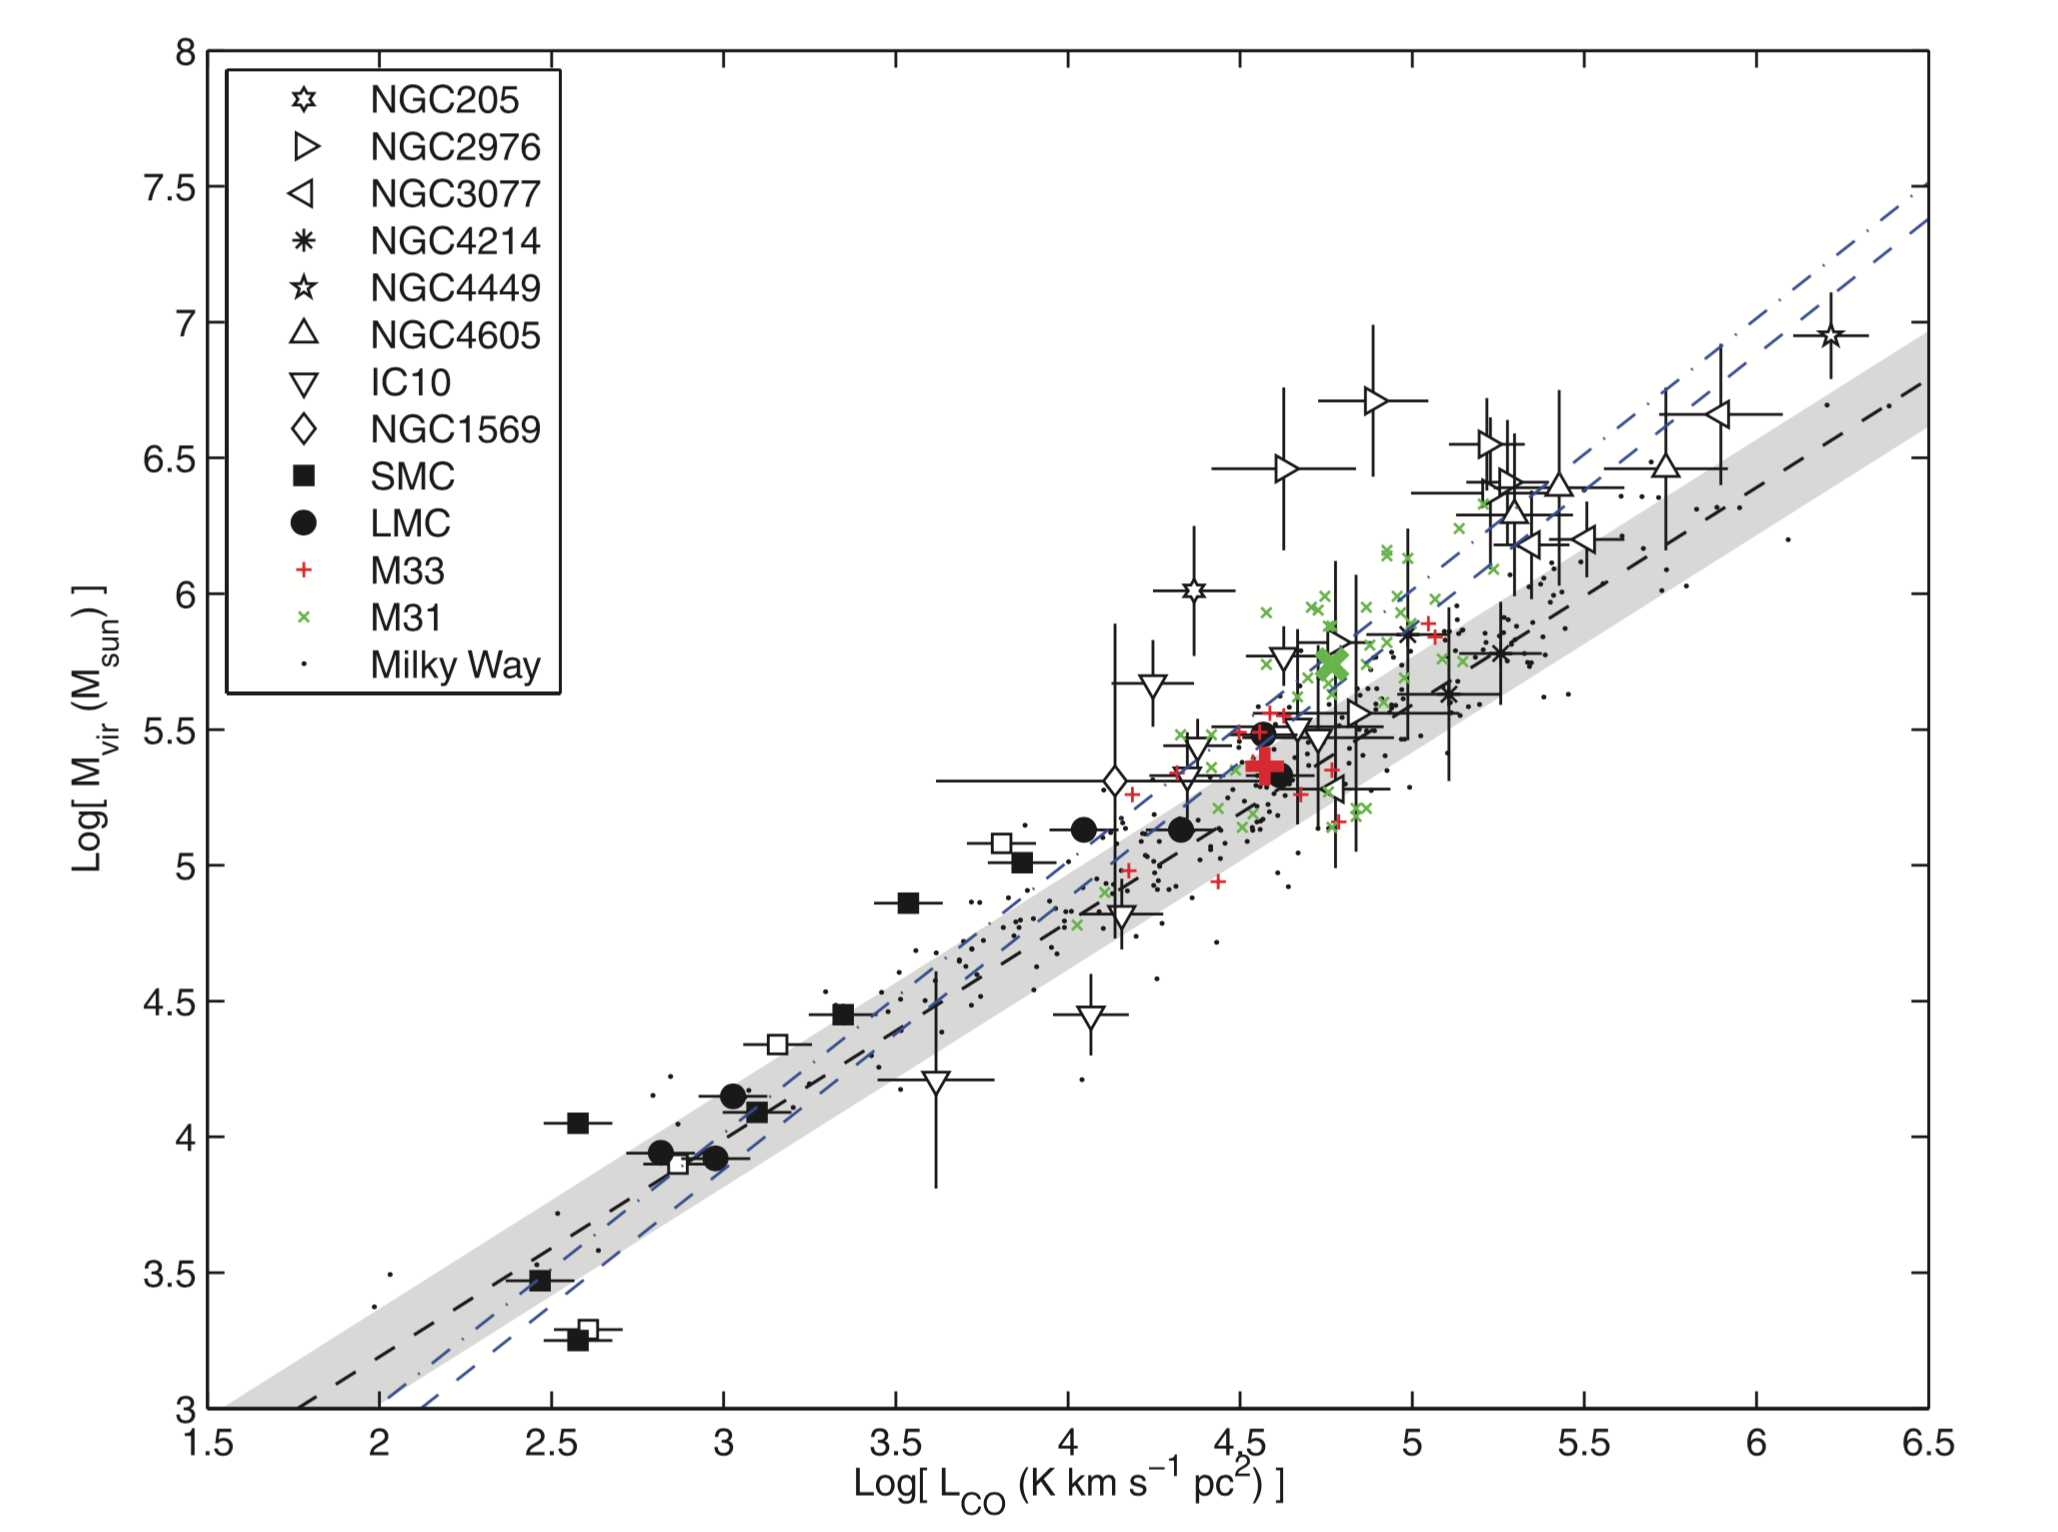
\includegraphics[width=\textwidth]{../image_intro/mvirial_lco.png}
\caption[Relation between the virial mass and CO luminosity]{Relation between the virial mass (M$_{\mathrm{vir}}$) and CO luminosity (L$_{\mathrm{CO}}$) for the Milky Way and extragalactic GMCs. The Milky Way data are shown by dots measured by~\cite{Solomon87}. Black and white symbols correspond to measurements based on $^{12}$CO~($J(2\rightarrow 1)$) and $^{12}$CO~($J(1\rightarrow 0)$), respectively. The black dashed line represents the Galactic mass-luminosity relation (M$_{\mathrm{vir}} \approx 39{\mathrm L}^{0.81}_{\mathrm{CO}}$) with gray region illustrating the Galactic 1$\sigma$ dispersion around the line.
The dot-dashed and blue dashed lines show the fits for dwarf sample and all extragalactic GMCs, respectively.
The extragalactic molecular clouds are very similar to those in the Milky Way. Adapted from~\cite{Bolato08}.}
\label{fig: mco}
\end{figure}

In order to empirically determine the relation between H$_2$ masses and CO luminosities, many observational attempts have been made on both Galactic and extragalactic scales. 
One of the most significant studies in this regard was done by~\cite{Solomon87}, who studied this relation over more than 273 clouds inside the Milky Way and found a strong correlation between the virial mass of molecular clouds and CO luminosity. 
In Local Group galaxies, several groups have measured size, line width, and CO luminosity of molecular clouds and investigated the relation between  their virial masses and CO emission in environments other than the Milky Way. 
Pioneering works in measuring the extragalactic conversion factor were done for M31 and M32~\citep[e.g.,][]{Wilson89, Wilson90}. 
Fig.~\ref{fig: mco} shows the CO luminosity versus virial masses of the Galactic and extragalactic molecular clouds. 
The extragalactic molecular clouds are similar to those in the Milky Way. 
The conversion between the CO luminosity and H$_2$ masses is still a controversial topic~\citep[e.g.][]{Narayanan11, Bolato13, Sandstrom13}.
Problems regarding metallicity are not yet resolved and it is still not clear whether the conversion factor is global or local. 
Extragalactic investigations have been limited to nearby galaxies due to telescope resolution and sensitivity. 
To measure the clouds in distant galaxies, the spatial resolution of maps must be better than 40~pc, which is the typical size of a giant molecular cloud~\citep[e.g.][and references therein]{Young91,Bolato13}. 

Atomic gas in galaxies is dominated by \hi~atoms, which are relatively easy to observe in 21-cm.
Assuming optically thin lines for \hi~emission, the intensity of the 21-cm emission is proportional to the density of the atomic hydrogen, $N_{H {\sc I}}$~(cm$^{-2}$), along the line-of-sight.
\begin{equation}
N_{H {\sc I}}  \propto \int T_{\mathrm B} dV
\end{equation}
where $T_{\mathrm B}$ is the temperature brightness in Kelvin and dV is in km~s$^{-1}$, with the integral over the line profile. 
These properties make the 21-cm line a very useful tool to study gas in the ISM and trace the large-scale distribution of galaxies in the universe (\hi~is detectable in most spiral galaxies and some elliptical galaxies).
Although the 21-cm emission is the most reliable technique to map the ISM, the linear relationship between the intensity and the column density of the gas breaks down when the gas is optically thick~\citep{Braun09}. 

\subsubsection{Dust Emission as a Tracer of Gas} 

Studying the gas clouds in the ISM of distant galaxies by using direct methods is almost impossible and not practical, due to low spatial resolution of available observational data.
\cite{Hildebran83} was the first to suggest that one way to estimate the mass of the gas in the ISM might be from the optical depth of the sub-mm continuum emission from the dust; continuum dust emission is generally optically thin. 
The Herschel Space Telescope~\citep{Pilbratt10} has measured the continuum dust emission from hundreds of galaxies~\citep{Eales10, Oliver12}. 
This amount of observational data provides a unique opportunity to study the ISM of galaxies using dust emission. 
The observed FIR flux has almost no dependency on distance, thus, one of the advantages of using the dust emission as a tracer of the gas mass is that unlike the direct method, high spatial resolution is not necessary. 
The other important advantage is that this method solves the newly-found problem of ``dark gas" in galaxies. 
Dark gas is a significant fraction of gas in galaxies which can be traced by neither the 21-cm emission nor the CO emission~\citep{Abdo10}. 
As such, it is very difficult to detect with telescopes, but an accurate gas to dust ratio can lead to an accurate estimate of dark gas mass in galaxies. 

There are disadvantages in using the gas to dust ratio to trace gas in the ISM.
In order to use the dust as a tracer of the gas mass, first a relationship between the optical depth and the mass of the dust and then a relationship between the mass of the dust and the mass of the gas must be derived.
\cite{Draine03} pointed out that the former approach is uncertain because of the uncertainly in the radiative efficiency of dust grains. 
Measuring the gas to dust ratio in galaxies are not accurate either~\citep{Hildebran83}, which means that there are problems in both steps. 
In addition, the dust method has two major practical problems: firstly, to apply this method, knowing the temperature of the dust is necessary. 
To solve this problem, measurement of the continuum emission at far-infrared wavelengths long enough to cover the peak of the emission must be very accurate~\citep{Ealas12}. 
The other problem is that there is evidence that the gas to dust ratio depends on the metallicity of the gas~\citep{Lisenfeld98, Draine07}, but even in direct methods the dependence on metallicity must be solved. 
Using dust emission as a tracer of gas is the best alternative for measuring the total gas in galaxies, that there is no observation of CO or \hi~emission. 

\subsection{The ISM and starlight: extinction and attenuation}
\label{sec: extinction}
Dust in ISM affects stellar emission by attenuating, scattering or absorption.
Effect of dust clouds with embedded light sources on distribution of the light is called attenuation. 
The dust cloud could have any distribution and be clumpy or smooth. 
Since both light source and dust have extended distributions, the relative locations of the dust and light source affect the net absorbed and scattered light.
The other parameter that is important for the scattering and absorption is the relative position of dust and observer.
When the dust is in the line of sight, attenuation will make the emerging light dimmer~\citep[e.g.][and references therein]{Calzetti13}.
This is the typically occurring situation when studying galaxies or extended regions within galaxies.

Extinction happens when there is a combination of both absorption and scattering of radiation by dust.
This effect grows inversely with wavelength.
%Extinction can be defined as a reduction of the original intensity caused by dust:
Extinction is quantified as the difference in observed and initial magnitudes of an object in a specific wavelength ($\lambda$):
\begin{equation}
m_{\lambda} - m_{\lambda}(0) = \mathrm{A}_{\lambda},
\end{equation}
where $\mathrm{A}_{\lambda}$ is the extinction, and $m_{\lambda}$ and $m_{\lambda}(0)$ are observed and initial magnitude, respectively.
Magnitude is related to intensity (I) as:
\begin{equation}
m_{\lambda} = 2.5 \log (I_{\lambda}) + C,
\end{equation}
where $c$ is a constant which depends on photometric system that is being used.
Optical depth, $\tau_{\lambda}$, is defined by ratio of observed and initial intensity of a source as:
\begin{equation}
\label{equ: extinction}
{\mathrm I}(\lambda) = {\mathrm I}_0(\lambda)\exp[-\tau_{\lambda}],
\end{equation}
where I$(\lambda)$ is observed intensity in wavelength $\lambda$ and I$_0(\lambda)$ is intensity of light before passing through dust.
Therefore, the optical depth and extinction can be converted to one an other by $\tau_{\lambda} = 1.086 \mathrm{A}_{\lambda}$. 
The extinction also depends on the grain size and extinction cross section.
For measuring SFR using various wavebands, decreasing of the intensity of radiation must be calculated and corrected for each wavelength; otherwise, there will be an underestimation of SFR. 

%%%%%%%%%%%%%%%%%%%%%%%%%%%%%%%%%%%%%%%%%%%%%%%%%%%%%%%%%%%%%%%%%%%%%%%
%%%%%%%%%%%%%%%%%%%%%%%%%%%%%%%%%%%%%%%%%%%%%%%%%%%%%%%%%%%%%%%%%%%%%%%
%%%%%SFR%%%%%%%%%%%%%%
%%%%%%%%%%%%%%%%%%%%%%%%%%%%%%%%%%%%%%%%%%%%%%%%%%%%%%%%%%%%%%%%%%%%%%%
%%%%%%%%%%%%%%%%%%%%%%%%%%%%%%%%%%%%%%%%%%%%%%%%%%%%%%%%%%%%%%%%%%%%%%%

\section{Measuring the star formation rate in galaxies} 
\label{sec: sfr_intro}
Understanding the formation of stars leads to better understanding of galaxies' formation and evolution. 
Characterisation of the star formation processes such as star formation rate (SFR) and the stellar initial mass function (IMF) is necessary in examining galaxies' structure formation~\citep{McKee07}. 
Measuring the SFR is not trivial and depends on a galaxy's morphology, metallicity, IMF, observational spatial resolution, and other properties. 
There is a large number of review papers on how stars form and how their formation is traced. 
From a theoretical perspective, one can refer to the classic picture of the theory of star formation as reviewed by \cite{Shu87} and more recently by~\cite{McKee07}. 
From an observational standpoint, star formation is discussed by many authers \citep[e.g.][and references therein]{Kennicutt98b, Kewley02, Calzetti13, Boquien10, Kennicutt12}.

In principle, emission from new stars can be traced by ultraviolet, visible light, near-IR and radio wavelengths, hydrogen recombination lines, forbidden metal lines, and also in the sub-mm range by using the Bremsstrahlung emission. 
Some of this emission is directly from stars, e.g.\ UV emission, and some is from ISM components that absorb and re-emit light from young stars, e.g.\ far-infrared emission.
Techniques to calibrate emission from newly-born stars, preferably hot and massive ones, to the rate at which stars are being formed have been the subject of many studies~\citep[e.g.][]{Calzetti07, Kennicutt11, Hao11,Bigiel08}. 
Peak of emission of young, hot, and massive stars is in UV wavelength, which makes them an ideal tracer of the current SFR.
One of the main assumptions in using the luminosity of massive stars is that the SFR has remained largely constant during the timescale probed by the specific wavelength which is being used as the tracer. 
By knowing the IMF, the number of massive stars can be used to extrapolate the total number of stars formed in a given star-forming region.
To have a reliable SFR indicator, the stellar IMF must be fully sampled to have at least one star in all mass bins (for more detail see Section~\ref{sec: imf}).
In general each tracer has some systematic errors, and one should decide which tracer is more accurate for a given system. 

\subsection{Stellar Initial Mass Function}
\label{sec: imf}
Stellar mass determines the important properties of a star, such as luminosity, lifetime and its evolutionary path. 
One of the most fundamental and difficult questions that a complete theory of star formation must answer is what is the stellar initial mass distribution of a star forming region.
Since most SFR calibrations use emission from stars in a specific mass range, it is necessary to know the stellar IMF to extrapolate to the full stellar population.
\cite{Salpeter55} empirically derived the stellar IMF from the observed stellar luminosity function of the Solar neighbourhood~\citep{Shu87}. 
He introduced a power-law IMF $\Phi$  in the form:
\begin{equation}
\label{equ: salp}
\Phi (\log M) = dN / d \log M \propto M^{-\gamma }
\end{equation} 
where $M$ is the stellar mass, $\gamma$ is a power-law index, and $N$ is the number of stars in the logarithmic mass range of $\log M$ to $\log M + d\log M$. 

In the late 1970s, it was recognised that the assumption of a the single power-law IMF over all stellar masses is not correct and might overestimate the number of low-mass stars~\citep{Kroupa93, Bastin10}. 
Since then, many groups have studied the stellar IMF and found different power-law relations (Fig.~\ref{fig: imf} ). 
Most SFR calibrations have the same assumption that the stellar IMF is constant across all environments and adopt it from the standard stellar IMF introduced by\ \cite{Kroupa01}:
\begin{equation}
\begin{split}
    \Phi (\log M) & \propto M^{-2.3}    \quad    (0.1 \le M(M{\odot}) \le 0.5)\\                  
           & \propto M^{-3.3}    \quad    (0.5 \le M(M{\odot}) \le 100)
\end{split}
\end{equation}
Although the Salpeter IMF produces more low-mass stars than the Kroupa IMF, they produce almost the same number of high-mass stars. 
Therefore, the SFR calibrations, which mostly trace massive stars in galaxies, based on the Kroupa IMF can be converted to the Salpeter IMF by multiplying the calibration constant by 0.67~\citep{Madau14}.
In a more recent study,~\cite{Weisz15} used data from the Panchromatic Hubble Andromeda Treasury program~\citep[PHAT][]{Dalcanton12} and showed that for nearby galaxies both Kroupa and Salpeter stellar IMFs overestimate the number of stars with masses greater than 8M$_\odot$.
\cite{Bastin10} reviewed the stellar IMF as derived from many observational results and showed that the stellar IMF is constant and universal, though there are uncertainties in different mass bins especially at the high-mass end. 

\begin{figure}
\centering
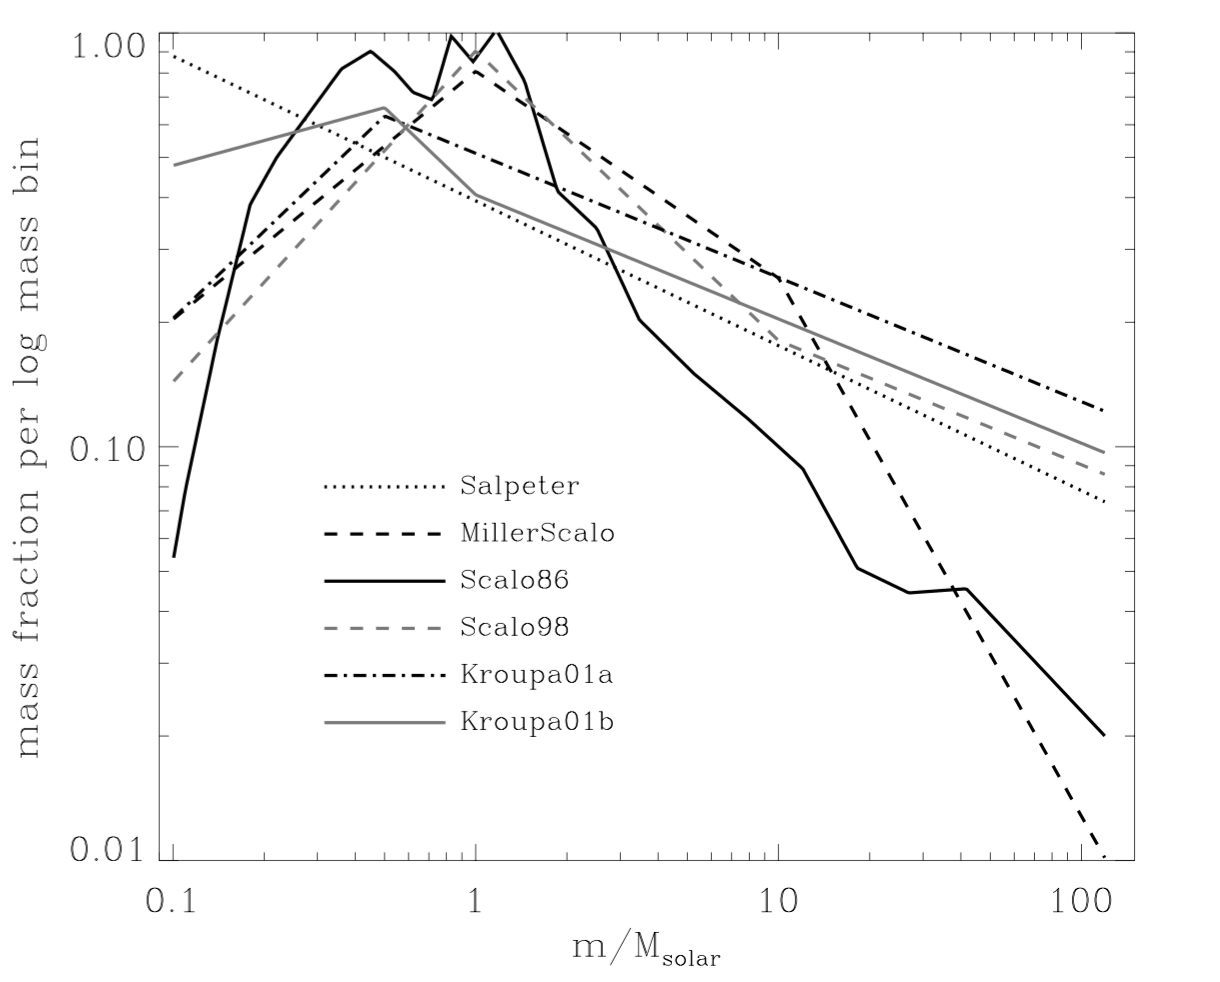
\includegraphics[width=16cm]{../image_intro/imf.png}
\small
\caption[Comparing stellar initial mass functions]{Comparing stellar initial mass functions (IMFs) by plotting the mass fraction per dex, power of 10, versus mass, normalized so that the integral under each curve is unity. The mass ranges from 0.1 to 120~M$_\odot$. Adopted from~\cite{Baldry03}.} 
\label{fig: imf}
\end{figure}


Since in using SFR calibration for different galaxies, I assume the initial mass function is universal, careful measurement of the IMF is the key factor in understanding the star formation rate. 
In distant galaxies, only massive stars can be detected; therefore, the IMF must be assumed to include all stellar mass ranges in the SFR calibrations. 
To show the impact of the different stellar IMF assumptions on the SFR calibrations, \cite{Calzetti13} used two different stellar IMFs and derived the SFR calibrations with these new assumptions.
Adopting a modified \cite{Kroupa01} IMF, with its maximum stellar mass set to 30~M$_{\odot}$ instead of 100~M$_{\odot}$, changes the SFR calibration constants by factors ranging from 1.4 to 5.6 for different SFR indicators (Table~\ref{table1}). 

\subsection{SFR Indicators}

One of the main issues in studying star formation in distant galaxies is the calibration of star formation rate indicators~\citep[e.g.,][]{Lee10}. 
Calibration of SFR indicators can be affected by differences in star formation history (SFH), metallicity, distribution of stellar population and dust in galaxies~\citep{Calzetti13}. 
Based on the spatial resolution of a system, one can divide star formation indicators into two categories: resolved and unresolved star formation indicators.

\subsubsection{Resolved Star Formation Indicators}
The most direct way to measure the SFR and trace recent star formation is counting individual objects~\citep{Kennicutt12}. 
These objects mostly few million years old and usually are referred to as young stellar objects (YSOs). 
Counting YSOs is used for calculating star formation rates in molecular clouds within $0.5- 1$~kpc of the Solar System. 
The number of YSOs can be converted to SFR using: 
\begin{equation}
SFR(YSO) = N_{yso} <M>/\tau 
\end{equation}
where SFR(YSO) is in units of M$_{\odot}$~yr$^{-1}$, N$_{yso}$ is the number of YSOs.
$<$M$>$ is the mean mass of YSO which depends on the IMF and considering current IMFs $<$M$> = $0.5~M$_{\odot}$ ~\citep[][]{Kennicutt12}. 
$\tau$ is the lifetime of the YSO  $\tau \sim 2$~Myr~\citep{Evans09}. 
Since our current devices cannot resolve individual YSOs, this method can only be applied to the Milky Way and its neighbourhood. 

In theory, for any system with high enough spatial resolution, counting YSOs can be used as a tracer of the star formation. 
However, considering the limited capabilities of the present instruments, YSOs in most regions beyond the Magellanic Clouds (satellite galaxies of the Milky Way at a distance of 0.05 Mpc) cannot be resolved. 
Therefore, most studies use the emission from the energetic young stars as a tracer of the SFR. 

%% and the continuation


\subsubsection{Unresolved Star Formation Indicators}

In star-forming regions farther away than the Magellanic Clouds, the spatial resolution of currently-available observations is not high enough to find all the young stellar objects. 
In unresolved systems, calibrating continuum or line emission at wavelengths sensitive to the young massive stars is the primary method of measuring SFR~\citep[e.g.,][]{Kennicutt98b, Kewley02, Bell03, Calzetti07, Calzetti08, Calzetti10, Calzetti13, Kennicutt07, Kennicutt09, Boquien10, Hao11, Kennicutt12}. 
\cite{Kennicutt98b} calibrated the luminosities of galaxies at specific wavelengths for measuring the SFR, using relations between the SFR per unit mass or per unit luminosity and the integrated colour of a system provided by stellar populations synthesis models~\citep[e.g.,][]{Bruzual93}. 

In unresolved systems, SFR indicators can be divided into local and global indicators. 
The global SFR indicators are defined for the entire galaxy; therefore, they are luminosity-weighted averages across local star formation history and the physical condition inside each galaxy. 
Local calibration is used for regions within a galaxy~\citep[e.g.,][]{Zhu08, Kennicutt09, Boquien10, Boquien11, Hao11}.
Limitations in the spatial resolution of observational data on the one hand, and the broader applicability to distant galaxy populations on the other, have in the past brought more attention to the calibrations of global SFR compared to local SFR. 
Because of its ability to trace the physical processes of the star formation, local SFR calibration is becoming increasingly important~\citep{Calzetti13}.

\subsubsection*{SFR Indicators Based on Single-Band Emission}

In order to derive conversions between the luminosity in specific wavelengths and the SFR, stellar population synthesis models are used~\citep{Kennicutt98b}. 
The general form of a SFR calibration using single-band emission is: 
\begin{equation}
\label{equ: sfrsingle}
{\rm SFR}(\lambda)= CL(\lambda),
\end{equation}
where SFR is in units of M${_\odot}$~yr$^{-1}$, $L(\lambda)$ is the luminosity in erg~s$^{-1}$ at the wavelength $\lambda$, and $C$ is a constant derived from stellar population models~\citep[e.g, starburst99][]{Leitherer99}). 
The constant $C$ varies for different wavelengths, mass ranges of the stellar IMF, and the timescale $\tau$ over which star formation is assumed to remain constant. 
Table~\ref{table1}, from \cite{Calzetti13}, summarises some values of $C$ and their changes according to different assumptions about the IMF. 


\begin{table}
\caption{Luminosity-to-SFR calibrations adapted from~\cite{Calzetti13}}
\label{table1}
\begin{center}
\begin{tabular}{ c c c }
\hline\hline
Luminosity$^1$ & C$^2$ & Assumptions$^3$\\
\hline
L$_{UV}$ & $3.0 \times 10^{(-47)} \lambda$ &$0.1 -100 M_{\odot}, \tau \ge 100 Myr $\\
L$_{UV}$ & $4.2 \times 10^{(-47)} \lambda$ &$0.1 -30 M_{\odot}, \tau \ge 100 Myr $\\
L$_{UV}$ & $4.3 \times 10^{(-47)}\lambda$ &$0.1 -100 M_{\odot}, \tau = 10 Myr $\\
L$_{UV}$ & $1.0 \times 10^{(-46)}\lambda$ &$0.1 -100 M_{\odot}, \tau = 100 Myr $\\
L(TIR) & $1.6 \times 10^{(-44)}$ &$0.1 -100 M_{\odot}, \tau = 100 Myr $\\
L(TIR) & $2.8 \times 10^{(-44)}$ &$0.1 -100 M_{\odot}, \tau = 100 Myr $\\
L(TIR) & $4.1 \times 10^{(-44)}$ &$0.1 -30 M_{\odot}, \tau = 100 Myr $\\
L(TIR) & $3.7 \times 10^{(-44)}$ &$0.1 -100 M_{\odot}, \tau = 100 Myr $\\
L(TIR) & $8.3 \times 10^{(-44)}$ &$0.1 -100 M_{\odot}, \tau = 100 Myr $\\
L(H${\alpha}$) & $5.5 \times 10^{(-42)}$&$0.1 -100 M_{\odot},  \tau \ge 6 Myr $\\
L(H${\alpha}$) & $3.1 \times 10^{(-41)}$&$0.1 -30 M_{\odot},  \tau \ge 10 Myr $\\
\hline
\end{tabular}
\end{center}
\begin{tablenotes}
\item $^1$ Luminosities (except for UV) are in erg~s$^{-1}$ and are given as $\nu L_{\nu}$.
\item $^2$ The constant $C$ appears in Equ.~\ref{equ: sfrsingle}. For SFR(UV), the numerical value is multiplied by the wavelength $\lambda$ in \AA to convert luminosity density to luminosity. 
\item $^3$ Assumptions for the mass range of the stellar IMF, using the expression derived by \cite{Kroupa01} (see Section~\ref{sec: imf}), and for the timescale $\tau$.
\end{tablenotes}
\end{table}


The most common single-band tracer of star formation rate is the ultraviolet.
As mentioned before, UV emission is an excellent tracer for the SFR.
Using a spectral energy distribution (SED) from Starburst99, with solar metallicity, and assuming a~\cite{Kroupa01} stellar IMF with the timescale of over 100 Myr, SFR can be measured as~\citep{Leitherer99}:
\begin{equation}
SFR(UV) = 3.0 \times 10^{-47}\lambda L_{\lambda}
\end{equation}
where SFR(UV) is in M$_{\odot}$~yr$^{-1}$, $\lambda$ can be in the range of $(912< \lambda < 3000~$\AA), and $L_{\lambda}$ is in erg s$^{-1}$\AA.
As shown in Table~\ref{table1}, with changes in the stellar ranges of the IMF, during timescales longer than 100 Myr, the calibration constant only decreases by a few per cent.
The calibration constants' changes for shorter timescales are more significant and 
the their accuracy is 15 per cent which can vary as a function of $\lambda$~\citep{Calzetti13}.
Ultraviolet light can easily be absorbed or scattered by interstellar dust. 
Therefore, using the UV emission as a tracer might lead to underestimation of the SFR if dust extinction corrections are not applied (\cite{Kennicutt12}; also see Section~\ref{sec: ism_intro}). 

Another single-band SFR indicator is the emission from hydrogen recombination lines. 
Ionizing photons emitted from young massive stars ionize the surrounding gas. Hydrogen recombination line emission, such as the Balmer series lines of H${\alpha}$ ($0.6563 \mu$m) and H${\beta}$ ($0.4861 \mu$m), which are located in the optical wavelength range, are among the most traditional SFR indicators~\citep{Kennicutt98a}. 
The relationship between the intensity of a hydrogen recombination line and the ionizing photon rate for a nebula is derived using quantum mechanics. 
The assumption is that the nebula must be optically thick to ionizing photons~\citep{Osterbrock06}.
Being optically thick means that almost all transitions more energetic than Ly${\alpha}$ absorb and re-emit via Ly${\alpha}$ and longer wavelengths.
This is why the H${\alpha}$ emission line strength is greater in optically thick environments. The relation between the SFR, the luminosity of the \halpha\ emission line, and the ionizing photon rate is~\citep[e.g.,][]{Osterbrock06, Kennicutt98b}:
\begin{align}
\label{equ: halpha}
SFR(H\alpha) = 5.5 \times 10^{-42}L(H\alpha) \\
                     = 7.4 \times 10^{-54}Q(H^{\circ})
\end{align}
where SFR(\halpha) is in M$_{\odot}$~yr$^{-1}$, L(\halpha) is in erg~s$^{-1}$, and Q(H$^{\circ}$) is the ionizing photon rate in units of s$^{-1}$.
The constant on the right-hand side of Equ.~\ref{equ: halpha} is the resulting coefficient for electron temperature T$_{\mathrm{e}}=10000$~K and density n$_{\mathrm{e}}=100$~cm$^{-3}$ which is typical in the \hii~regions.
Dust extinction (Section~\ref{sec: ism_intro}) is the most important source of systematic error in calculating the SFR from hydrogen recombination lines.
The effects of dust must be measured and \halpha\ observations must be corrected for extinction (e.g. by adding lumincity at 24~$\mu$m (L(24~$\mu$m)) to account for dust emission) or this could lead to underestimating the SFR~\citep{Kennicutt98b}.


Another nebular line used as a tracer of the SFR is \oii~$\lambda$3727~\AA. 
Although the luminosities of forbidden lines do not correlate with the ionizing atoms directly, their extinction has a correlation with the \halpha\ emission. 
As a result, \oii~luminosity can be used as a tracer of the SFR through \halpha\ luminosity. 
\cite{Gallagher89} calibrated the SFR based on the \oii~luminosity by using a sample of 75 galaxies. 
Another calibration for this luminosity was derived by \cite{Kennicutt92}. 
In his review on the SFR,~\citep{Kennicutt98b} averaged these calibrations and derived the following relation:
\begin{equation}
SFR([O\ II]) = 1.4 \times 10^{-41} L([O\ II])
\end{equation}  
where SFR(\oii) is in M$_{\odot}$~yr$^{-1}$ and L(\oii) is in erg~s$^{-1}$.
Although SFR(\oii) is not as accurate as the SFR(\halpha), it is one of major SFR indicators in high-redshift galaxies.
In these galaxies, the \halpha\ emission line is redshifted out of the optical band.
Consequently, calibration of the strongest emission feature in the blue (\oii) as an SFR indicator is very useful~\citep{Kennicutt98b}.


Since interstellar dust absorbs approximately half of the starlight and re-emits in the infrared, the infrared emission can be used to trace the SFR.
The IR luminosity of a system depends not only on the amount of embedded dust, but also on the heating rate provided by the stars. 
Since young stars heat the dust to higher mean temperatures than old stellar populations, to first order, the shape of the thermal IR SED depends on the starlight SED~\citep{Helou86}.
The fact that the heating rate provided by the young stellar population is higher than the old stellar population indicates that dust heated by the former is more luminous and consequently its SED peaks at shorter wavelengths (observationally $\approx 60~\mu$m) in comparison with dust heated by old or low-mass stars.
Therefore, infrared observations are able to detect the emission from the dust heated by young stellar populations, and can be used as an SFR indicator.  

Two empirical single-band infrared star formation rate indicators are the 24~$\mu$m and 70~$\mu$m bands.  
The use of these two bands depends on the type of the galaxy under study or the physical environment in different regions within the galaxy. 
Since the luminosity of a stellar population with constant star formation increases with time, the IR emission, which is used as a tracer of the emission of the stellar population, has different calibration constants in the case of a global (the entire galaxy SFR indicator) or a local indicator.
That is because the global case includes the integrated stellar population of a galaxy, while the other is calculated from regions with short star formation timescales such as \hii~regions, large star-forming complexes, etc.~\cite{Calzetti13}.
Table~\ref{table2} shows the constant $C$ from Equ.\ref{equ: sfrsingle} for 24~$\mu$m and 70~$\mu$m luminosities, for local (spatial scale $\sim500$~pc for 24~$\mu$m and $\lesssim 1$ kpc for 70~$\mu$m) and global cases. 
\begin{center}
\begin{table}
\caption{Infrared luminosity to star formation rate calibrations}
\label{table2}
\begin{tabular}{ c c c c }
\hline\hline
Luminosity$^1$ & $C$ & Assumptions & References\\ 
\hline
L(24)$^{0.885}_{local}$ & $1.31 \times 10^{-38}$ &$1.10\times 10^{40} \le L(24) \le 3.10\times 10^{44}$&  \cite{Calzetti07}   \\ 
L(24)$_{global}$ & $2.04 \times 10^{-43}$ &$ 4.10\times 10^{42} \le L(24)  \le 5.10\times 10^{43}$& \cite{Calzetti07} \\
L(70)$_{local}$ & $9.4 \times 10^{-44} $ &$5.10\times 10^{40} \le  L(70) \le 5.10\times 10^{43}$& \cite{Li12} \\
L(70)$_{global}$& $5.9 \times 10^{-44}$ &$L(70) \ge 1.4 \times 10^{42} $& \cite{Li10}\\
\hline
\end{tabular}
\begin{tablenotes}
\item $^1$ Luminosities are in the form of L($\lambda$) = $\lambda$ L$_{\lambda}$ in erg s$^{-1}$.
\end{tablenotes}
\end{table}  
\end{center}



\subsubsection*{SFR Indicators Based on Multi-Band Emission}

%%add PAHs here
Despite the usefulness of having single-band SFR tracers, in many cases the corrections due to dust effects and luminosity ranges increase the uncertainty in measurements.
Nowadays, thanks to large surveys, enormous amounts of data are available at different wavelengths for galaxies, which allows for combining the emission from different bands and finding new calibrations.
The conversion between SFR and luminosities in multiple bands mostly helps to avoid problems regarding dust extinction or attenuation (see~\ref{sec: ism_intro}). 
The simplest possible way to combine luminosities at different bands in order to convert them to SFR is through a linear relation, for which the correlation with the SFR is empirically derived~\citep{Kennicutt12}.

The emission from dust heated by young stars changes by the amount of high energy photons emitted toward the dust and by the properties of the dust such as the grain size.
Therefore, calibration of SFR varies for each of the single-band IR emissions.
Assuming that dust heating is dominated by emission from young stars, integrating over the full wavelength range of the infrared part of the spectrum reveals the total infrared (TIR) emission of the system, which can be used as an SFR indicator~\citep{Kennicutt98b}. 
 
TIR luminosity can be measured from the integrated infrared SED or a calibration of spatially-resolved infrared photometry introduced by~\cite{Draine07}. 
\cite{Boquien10} modified calibration of the total infrared luminosity as: 
\begin{equation}
L(\rm TIR) = 0.95L(PAH 8 \mu m) + 1.15L(24 \mu m) + L(70 \mu m) + L(160 \mu m),
\end{equation}
where $L = \nu L_{\nu}$ is the luminosity in erg~s$^{-1}$ at frequency $\nu$. 
\cite{Calzetti07} indicated that the star formation rate calibration for a stellar population undergoing constant star formation over $\tau=$100~Myr is:
\begin{equation}
\label{sfr_tot_IR}
SFR(\rm TIR) = 2.8 \times10^{-44}L(\rm TIR),
\end{equation}
where SFR(TIR) is in M${\odot}$~yr$^{-1}$, and L(TIR) is in erg~s$^{-1}$. 


In Sec~\ref{sec: overview} I mentioned that emission from PAHs in ISM can be used as an SFR indicator~\citep[e.g.][]{Peeters04}.
Most studies used emission in broad infrared bands, which contain PAHs, to calibrate SFR~\citep[e.g.][]{Calzetti07}, but SFR can be calibrated using only the PAH features.
\cite{Shipley16} calibrated SFR using observations from 105 star-forming galaxies with $z < 0.4$ as:
\begin{equation}
\log SFR = A + B \log L_{\mathrm{PAH}, \lambda},
\end{equation}
where $L_{\mathrm{PAH}, \lambda}$ is the luminosity of the PAH features at 6.2, 7.7, 11.3~$\mu$m or combinations thereof, in erg~s$^{-1}$.
Table~\ref{table_PAH} shows the constants for each $L_{\mathrm{PAH}, \lambda}$.
These calibrations underestimate the SFR for low-redshift galaxies with IR luminosity more than $10^{12}$~erg~s$^{-1}$.
\cite{Shipley16} showed that using the 7.7~$\mu$m feature in the calibration reduces the scatter and concluded that this wavelength provides the most robust SFR tracer.


\begin{table}
\caption{SFR calibrations from PAH luminosities; adopted from~\cite{Shipley16}}
\label{table_PAH}
\begin{center}
\begin{tabular}{ l c c}
\hline\hline
PAH Feature(s) & A & B\\
\hline
6.2 + 7.7 + 11.3 & $ -42.56 \pm 0.03 $ &  $1.00 \pm 0.03$ \\ 
6.2 & $ -40.06 \pm 0.09 $ &  $0.96 \pm 0.04$ \\ 
7.7 & $ -42.38 \pm 0.06 $ &  $1.00 \pm 0.03$ \\ 
11.3 & $ -44.14 \pm 0.08 $ &  $1.06 \pm 0.03$ \\ 
6.2 + 7.7 & $ -42.05 \pm 0.04 $ &  $0.99 \pm 0.03$ \\ 
6.2 + 11.3 & $ -42.52 \pm 0.05 $ &  $1.01 \pm 0.03$ \\ 
7.7 + 11.3 & $ -42.85 \pm 0.04 $ &  $1.01 \pm 0.03$ \\ 
\hline
\end{tabular}
\end{center}
\end{table}  


The most common use of combining luminosities to trace the SFR is the combination of total infrared measurements with both far- and near-ultraviolet observations, with the latter being more commonly used. 
This combination helps to avoid uncertainties from corrections for dust attenuation in far-UV (FUV) observations~\citep[e.g.][]{Hao11}. The calibration is:
\begin{equation}
L_{FUV}(\rm corr) = L_{FUV}(\rm obs) + \alpha L_{\rm TIR},
\end{equation}
where the luminosities are $L = \nu L_{\nu}$ in erg~s$^{-1}$, and the coefficient $\alpha$ depends on the bandpasses chosen for the UV and IR measurements. $\alpha$ is usually less than 1 because significant amounts of IR emission in many galaxies are from dust heated by older populations of stars~\citep{Kennicutt12}. The coefficient $\alpha$ is calibrated both theoretically, using evolutionary synthesis models, and empirically, by using measurements of dust corrected SFRs~\citep[e.g.][]{Hao11, Leroy08}. 

Another common method for using the multi-wavelength indicator for star formation is using H${\alpha}$ emission in combination with the 24~$\mu$m emission. 
This combination gives a more accurate dust-corrected estimate of the SFR~\citep{Kennicutt09}:
\begin{equation} 
\label{equ: halphaplus24}
SFR = 7.9 \times 10^{-42}[L(H{\alpha})_{\rm obs} + 0.020L(24 \mu m)]
\end{equation}
where L(H${\alpha}$)$_{\rm obs}$ is the observed H${\alpha}$ luminosity without correction for internal dust attenuation, given in the unit of erg~s$^{-1}$. 
L(24) is the 24~$\mu$m IR luminosity in erg~s$^{-1}$, and SFR is in M$_{\odot}$~yr$^{-1}$.


The IR emission in the other band can be used for correcting dust effect on UV or \halpha emission (see Table~\ref{table3}). 
The corrected emission then can be used as a SFR tracer.
These composite SFR indicators also have systematic uncertainties; yet, it seems that there is a good correlation between multi-band tracers and single-band tracers. 
Moreover, less uncertainty arises in this case than when using the single-band emission as a tracer~\citep{Kennicutt09}. 


\begin{table}
\caption{Multi-wavelength dust-corrected luminosities, adopted from~\cite{Kennicutt12}}
\label{table3}
\begin{center}
\begin{tabular}{ c}
\hline\hline
Combined luminosities$^1$ \\
\hline
L(FUV)$_{\rm corr}$=L(FUV)$_{\rm obs}$ + 0.46L(TIR)$^2$\\
L(FUV)$_{\rm corr}$=L(FUV)$_{\rm obs}$ + 3.89L(24~$\mu$m)$^2$\\
L(NUV)$_{\rm corr}$=L(NUV)$_{\rm obs}$ + 0.27L(TIR)$^2$\\
L(NUV)$_{\rm corr}$=L(NUV)$_{\rm obs}$ + 2.26L(24~$\mu$m)$^2$\\
L(\halpha)$_{\rm corr}$=L(\halpha)$_{\rm obs}$ + 0.0024L(TIR)$^3$\\
L(\halpha)$_{\rm corr}$=L(\halpha)$_{\rm obs}$ + 0.020L(24~$\mu$m)$^3$\\
\hline
\end{tabular}
\end{center}
\begin{tablenotes}
\item $^1$ Luminosities are in the form of L($\lambda$) = $\lambda$ L$_{\lambda}$ in erg~s$^{-1}$ 
\item $^2$ Calibrated by~\cite{Hao11}
\item $^3$ Calibrated by~\cite{Kennicutt09}
\end{tablenotes}
\end{table}  


As mentioned in Section~\ref{sec: imf}, using different IMFs results in having different calibration constants for star formation rate. 
From Table~\ref{table1} it is clear that changing the IMF affects the H${\alpha}$ SFR calibration more than other SFR calibrations. 
This effect is more than four times larger than for UV SFR calibrations because newly-formed stars having up to $\sim 5$ M$_{\odot}$ emit more strongly at UV wavelengths than any other part of the spectrum; however, significant amounts of ionising photons are produced by stars more massive than $\sim 20$ M$_{\odot}$.
Furthermore, reaching an asymptotic value of ionizing photons takes longer for more massive stars (10 Myr for the upper mass limit of 30 M$_{\odot}$ versus 6 Myr for 100 M$_{\odot}$). 
Therefore, changes in the H${\alpha}$ SFR calibration constant are more pronounced, while for UV and TIR the calibration constants are fairly close to each other.
On the other hand, using the mean stellar mass for the Kroupa IMF $(<$M$> \sim 0.6$ M$_{\odot})$ yields less than a 10\% difference between using the upper mass limit of 100 M$_{\odot}$ and 30 M$_{\odot}$. 
As a result, calibrations derived with the mean stellar mass of a system are more accurate than those that are based on tracing the most massive stars~\citep{Calzetti13}.

Our understanding of star formation in extragalactic systems depends on the light emitted by those systems.
While emissions from massive and young stars are the dominating light of the system, mass of low-mass stars dominates the mass of the regions (see Section~\ref{sec: imf}).
Therefore, SFRs are calibrated based on the dominant light of the systems and low-mass stars are accounted for using the initial mass function.
Emission from star forming regions should be corrected before it can be used in calibrations.
On its way to the Earth this emission passes through dust and gas clouds which cause extinction or attenuation (see ref.~\ref{sec: extinction}).
On the other hand, evolved stars emit their light in the whole spectrum as well as the  UV. 
Therefore, even though it might have an insignificant part in UV emission from galaxies, a correction for emission from evolved stars should be considered~\citep{Leroy08}.
After measuring the corrected luminosities for star forming regions in galaxies (global or local), using proper calibrations can give the best estimation of SFR in galaxies. 




%%%%%%%%%%%%%%%%%%%%%%%%%%%%%%%%%%%%%%%%%%%%%%%%%%%%%%%%%%%%%%%%%%%%%%%
%%%%%%%%%%%%%%%%%%%%%%%%%%%%%%%%%%%%%%%%%%%%%%%%%%%%%%%%%%%%%%%%%%%%%%%
%%%%%Stellar Mass%%%%%%%%%%%%%%
%%%%%%%%%%%%%%%%%%%%%%%%%%%%%%%%%%%%%%%%%%%%%%%%%%%%%%%%%%%%%%%%%%%%%%%
%%%%%%%%%%%%%%%%%%%%%%%%%%%%%%%%%%%%%%%%%%%%%%%%%%%%%%%%%%%%%%%%%%%%%%%

\section{Stellar mass}
\label{sec: starmass_intro}
One of the most fundamental physical parameters that describes the present state of a galaxy is its stellar mass. 
Stellar mass is linked to the structure and star formation history of disc galaxies~\citep{Gavvazi96} and  galaxies of all morphologies~\citep{Scodeggio02}. 
Measuring the mass of a stellar population is indirect and subject to significant uncertainties. 
In principle there are two ways to measure stellar mass in galaxies. 
The first is measuring the dynamical mass of a galaxy using kinematics (the motion of stars)~\citep{Cappellari06} or gravitational lensing (the bending of light as it passes near a galaxy)~\citep{Auger09}, and then modeling the mass of the dark matter and subtracting it from the measured mass. 
The second method is based on stellar population models~\citep[e.g.][]{Bruzual93, Kotulla09} and using them to connect stellar mass to an observable, such as luminosity in different wavelengths, colours, or spectral energy distribution. 
Stellar population models predict the expected SEDs for stellar populations based on the parameters of the regions such as star formation history, metallicity, and IMF.
Uncertainties come from the uncertainties in the stellar initial mass function (see Section~\ref{sec: imf}), the stellar evolution models (especially the stage where stars have the most luminosity in their evolution), the evolutionary state of the galaxy~\citep[see][and references therein]{Dalcanton12}, and star formation histories. 


In order to translate between photometry and stellar mass, the stellar mass-to-light ratio ($M/L$) is needed.
The use of $M/L$ is one way to measure the stellar mass surface density. 
It is an indirect method and has high uncertainties in specific cases, but can help in studying the stellar mass in large samples. 
For integrated galaxy light, the $M/L$ is estimated using scaling relations between $M/L$ and broadband colours \citep[e.g.][]{Bell03}, and then multiplying this ratio by luminosity to estimate the mass.
For resolved galaxies, one can produce a map of the stellar mass surface density distribution in galaxies using resolved colours to measure spatial variations in $M/L$.
This method gives more accurate results than measuring the stellar mass surface density distribution from single-band images that are rescaled by a uniform mass to light ratio~\citep{Zibetti09}.

Comparing results from independent methods to measure stellar mass helps to determine whether there are any systematic differences.
Comparing the results from measuring stellar mass within galaxies shows that the differences are on the order of a few tens per cent~\citep{McLaughlin05}.
Therefore, to model subtleties, the advantages and disadvantages of using each method should be carefully considered. 


\subsection{Galaxy masses from dynamics}

The simplest and the most common way to estimate the mass of a galaxy is to assume that the dynamics of the galaxy are governed by simple Newtonian classical physics.
In this model, the circular velocity $v_{\mathrm{circ}}(r)$ of an orbit with radius $r$ within a spherical system of gravitational potential $\phi$ and mass $M$ is given by:
\begin{equation}
\label{eq: simpmass}
v^2_{\mathrm{circ}}(r)=r\frac{d\phi}{dr} = G\frac{M(r)}{r},
\end{equation}
where $G$ is the gravitational constant and $M(r)$ is the total mass within a sphere of radius $r$. 
For a flattened disk, which is the case in most spiral galaxies, the right hand side of Equ.\ref{eq: simpmass} is replaced by the more exact expression derived by~\cite{Freeman70}. 
For the case of no dark matter or bulge, \cite{Freeman70} showed that the rotation curve of a self-gravitating disk is:
\begin{equation}
v^2_{\mathrm{circ}}(R)= 4\pi G \Sigma_{0}R_{d} y^2[I_0(y)K_0(y) - I_1(y)K_1(y)],
\end{equation}
where $R$ is the distance from the centre, $\Sigma_0$ the central surface brightness, $R_d$ is the disk scale length where the ratio of the intensity of disk to bulge is equal to $e$.
$y$ is equal to $\frac{R}{2R_d}$, and $I_i(y)$ and $K_i(y)$ are  modified Bessel functions of the first and second kinds. 


The mass distribution in disk galaxies is usually calculated from rotation curves or integrated line profiles from emission lines such as H${\alpha}$, CO, or \hi. 
Integrated line widths only yield an estimate of total mass within some (uncertain) isophotal radius.
Thanks to the current generation of detectors, it is now possible to obtain very high-resolution spectra in the \halpha and CO lines over the most of the optical disks of galaxies.

A detailed description of calculating dynamical masses in galaxies is beyond the scope of this work. 
The methods mentioned here represent the first order of approximation. 
For more accurate results, one should consider non-circular rotational velocities and the fact that galaxies contain millions of stars plus interstellar objects; therefore simple two-object Newtonian physics is not sufficient. 
A detailed review of dynamical masses of galaxies can be found in \citet{Courteau13}.

\subsection{Galaxy masses from stellar population modelling}

Galaxies can be observed because of their stellar emission; stars radiate the energy produced from nuclear reactions in their cores. 
Given a star's initial mass, the theory of stellar evolution can describe the amount of released energy. 
Hence, stellar mass that is responsible for radiation of stars can be derived by modelling the spectral energy distributions of galaxies. 
However, some fraction of the mass of galaxies consist of evolved stars which no longer emit radiation yet still contribute to the galaxy mass as stellar remnants and should be considered in the models.
Stellar population synthesis models are used to predict the SED of a stellar population using many physical parameters. 
Some of these parameters, which control the time evolution of the stellar population, are age ($t$) of the population measured in years (also referred to as the time passed since the star formation began), IMF, and metallicity~\citep{Courteau13}.

The basic idea behind finding a suitable calibration between flux/luminosity of the stars in different wavelengths and stellar mass is that one can use the SFHs recovered from synthesizing the stellar optical colour-magnitude diagrams in different regions of a galaxy. 
The calculated stellar mass in nearby galaxies can be used to calibrate the fluxes from the stars in other galaxies.
\cite{Zibetti09} suggested that to reach the maximum spatial resolution one can recombine the photometric information on a pixel-by-pixel basis. 
They used this method to study the stellar mass distribution in galaxies as well as the dependence of the SED on stellar mass density.
To do so the surface density of stellar mass at each position is derived by 
\begin{equation}
\label{equ: massphot}
\Sigma_{{\mathrm M_\star}} (\alpha, \delta) = \Sigma_{\lambda}(\alpha, \delta) \gamma_{\lambda}(\alpha, \delta),
\end{equation}
where $\alpha$ and $\delta$ are sky position (right ascension and declination, respectively).
$\Sigma_{{\mathrm M_\star}} (\alpha, \delta)$ is the stellar surface density.
$\Sigma_{\lambda}(\alpha, \delta)$ is the surface brightness and $\gamma_{\lambda}(\alpha, \delta)$ is the effective stellar $M/L$ at an effective wavelength $\lambda$.
In Equ.\ref{equ: massphot},  $\gamma_{\lambda}$ can be described as a function of one or more colours as observed at the specified location in galaxy. 

The peak of emission from evolved stars is in the near-infrared part of the spectrum.
Therefore, many studies have tried to make a map of stellar mass distribution using this bandpass within galaxies~\citep[e.g.,][]{Elmgreen84}.
Thanks to the \Spitzer~\citep{Wener04} and WISE~\citep{Wright10} space telescopes, a large amount of data in these bands from many regions in the sky is available, which helps to give a more accurate calibration. 
Fluxes from 3.6 and 4.5~$\mu$m are suitable for calibration of the stellar mass, due to fact that these two band-passes not only trace evolved stellar population but are also almost insensitive to the emission from young stellar population and to dust absorption and emission. 
\cite{Zhu10} used the Sloan Digital Sky Survey~\citep[SDSS][]{York00} and the \Spitzer Wide-area Infrared Extragalactic Survey~\citep[SWIRE;][]{Lonsdale03} to find a calibration between galaxy luminosity and stellar mass. 
Using the $M/L$ of galaxies, they found correlations between $K_s$ band (2.2~$\mu$m), 3.6 and 4.5~$\mu$m band luminosities and stellar masses and formulated these correlations as:
\begin{equation}
\begin{split}
\label{equ: zhu1}
\log M_{\star} =& -1.60  + 1.12  \log \nu L_{\nu}[K_s]\\
\log M_{\star} =& -0.79 + 1.19 \log \nu L_{\nu}[3.6\mu \rm m]\\
\log M_{\star} =&-0.25 + 1.15\log \nu L_{\nu}[4.5\mu \rm m], 
\end{split}
\end{equation}
where M$_{\star}$ is the stellar mass in solar masses and $ \nu L_{\nu}[\lambda]$ is the luminosity in erg~s$^{-1}$ at a specified wavelength.

\cite{Eskew12} tested the 3.6- and 4.5 $\mu$m fluxes as proxies for stellar mass in the Large Magellanic Cloud and found an empirical relation between mass of the stars and the luminosities of stars as:
\begin{equation}
\label{equ:eskew}
  M_{\star} = 31.84 \times 10^{5.65} L_{3.6}^{2.85} L_{4.5}^{-1.85},
\end{equation}
where M$_{\star}$ is the stellar mass in solar masses, and $L = \nu L_{\nu}$ is luminosity in erg~s$^{-1}$~\AA$^{-1}$.
Equ.s in~\ref{equ: zhu1} were derived from a large sample of galaxies and tested on different types of regions and galaxies.
On the other hand,~\cite{Eskew12} mentioned that since their calibration is based on data from the Magellanic Clouds,
measuring the stellar mass from Equ.~\ref{equ:eskew} might break down for highly star-forming regions; moreover, this equation has not been tested on regions with different metallicities. 
%In more recent work,~\cite{Laura16} measured stellar mass for a group of galaxies with ($z < 0.035$) using correlation introduced by~\cite{Eskew12} and showed these stellar masses are tightly correlated with stellar masses measured from other calibrations.
In more recent work,~\cite{Laura16} measured stellar mass for a group of galaxies with $z < 0.035$, using the correlation that was introduced by~\cite{Eskew12}. 
The study revealed that measured stellar masses in that study are tightly correlated with stellar masses measured from other calibrations.
%%%%%%%%%%%%%%%%%%%%%%%%%%%%%%%%%%%%%%%%%%%%%%%%%%%%%%%%%%%%%%%%%%%%%%%
%%%%%%%%%%%%%%%%%%%%%%%%%%%%%%%%%%%%%%%%%%%%%%%%%%%%%%%%%%%%%%%%%%%%%%%
%%%%%Preview%%%%%%%%%%%%%%
%%%%%%%%%%%%%%%%%%%%%%%%%%%%%%%%%%%%%%%%%%%%%%%%%%%%%%%%%%%%%%%%%%%%%%%
%%%%%%%%%%%%%%%%%%%%%%%%%%%%%%%%%%%%%%%%%%%%%%%%%%%%%%%%%%%%%%%%%%%%%%%

\section{Preview}
\label{sec: pre_intro}

A complete picture of how galaxies are formed and evolve is tied to unfolding the mystery of the formation of stars.
Various phenomena affect the collapse of molecular clouds and star formation, including the environment of the star-forming region, chemical composition of the region, the initial density distribution of the gas and the mass of stars in galaxies.
For decades, observational, theoretical, and numerical studies have investigated star formation; nevertheless, their results are not in agreement.
Empirical studies are used alongside theoretical ones to find laws that indicate the relations between physical properties of galaxies and star formation.

The most well-known scaling law is the relation between the surface densities of the star formation rate and the gas mass, known as the Kennicutt-Schmidt (K-S) law~\citep{Schmidt59, Kennicutt98a}. 
The K-S law and similar empirical laws have been tested on local and high-redshift galaxies with various morphological types, local and global scales and different ISM types~\citep[e.g.][]{Kennicutt08,Bigiel08,Genzel10,Gnedin10,Shi11}.
Despite all these studies, many questions about star formation laws still remain unanswered; the limitations of star formation laws are still undetermined and there is no definitive answer to whether or not there is a universal star formation law.
Their dependence on physical properties of galaxies is nontrivial, and sometimes differs by the type of star forming region.
Although a relation between star formation and gas is well established, the details of this relation are not clear:
different types of gas affect SFR in different ways, and variations in metallicity alter the effects.
There is no fully sampled and universal IMF, in fact there is an ongoing debate on whether the IMF is universal or not.
The influence of evolved stars and distance of star forming regions from the centre of galaxies on SFR has been mentioned in studies but not fully investigated.
Besides studying the impact of the aforementioned properties of galaxies on SFR, searching for other relations between properties of galaxies and their star forming regions continues.

Advances in observing facilities, image quality, and methodology expand our knowledge of star formation. 
In the past few decades, the use of advanced statistical methods in astronomical studies has also grown.
Applying modern statistical methods to star formation studies can shed light on unsolved problems in this field. 
Studies show that using different statistical methods can change our perspective on star formation laws. 
For example,~\cite{Shetty13} used Bayesian methods to show that the K-S law is not universal. 
Since astronomy is a data-driven science, data-mining methods can be quite useful to gain new insights on properties of star-forming regions. 
However, these methods have not been widely-applied to studies of nearby galaxies, where the most detailed information about star formation is available.

In this thesis, I present three projects that study the effects of galaxy properties on star formation.
I use UV to radio observations of both nearby and high-redshift galaxies, measure their physical properties, and using modern statistical methods, study their impact on SFR.
Chapter~\ref{ch: paper1} focuses on investigating star formation laws in the Andromeda galaxy (M31) on both local and global scales using hierarchical Bayesian analysis.
In addition to the Kennicutt-Schmidt law, I study the extended Schmidt law~\citep{Shi11} and the metallicity/star formation correlation~\citep{Krumholz09}.
I also show the effect on star formation laws by using different SFR and ISM gas tracers.
In Chapter~\ref{ch: paper3}, I explore nearby galaxies using an unsupervised data-mining method (the self-organizing map, or SOM).
I cluster observational data to derive quantities of spatially resolved regions in M31 and examine the physical properties of each cluster.
During this process, I find hidden structures in high-dimensional data space.
In Chapter~\ref{ch: paper2}, I move to more distant galaxies and apply the SOM algorithm to their spectral energy distributions.
I train networks using a set of galaxy SED templates covering the wavelength range from UV to IR and use them to classify the SEDs of a sample of 142 galaxies with $0.5 < z < 1$. 
Then I study the grouped properties of the classified galaxies.
I summarize these results and discuss potential future work and applications of the results of this thesis in Chapter~\ref{ch: summary}

\addcontentsline{toc}{section}{Bibliography}
\bibliographystyle{apj.bst} 
\bibliography{ref_intro}
\chapter[Star formation laws in M31]{Star formation laws in the Andromeda galaxy: gas, stars, metals and the surface density of star formation}
\label{ch: paper1}


\section{Introduction}
\label{sec: intro_sfl}
%P1: Star formation laws and why they are important (introducing K-S law and E-S law)

Understanding the underlying processes of formation of stars is a necessary step for explaining the formation and evolution of galaxies from the early universe to the current epoch, as well as the origin of planetary systems. Stars form when molecular cloud cores collapse; however, a complete picture explaining the physical processes involved in the formation of stars is yet to emerge. Various phenomena trigger the collapse of molecular clouds and star formation including the environment of the star-forming region, gas accretion and cooling, H$_2$ formation, the initial mass distribution and chemical compositions of the gas,  existence of dust, and other quantities in a galaxy. The physical processes leading to the formation of stars are naturally complex. Therefore, the basis for a theory of star formation requires a strong foundation of empirical data and/or observations.


The first attempt at scaling the star formation rate was to find a relation between the total star formation rate (SFR) and the mass of interstellar gas. \citet{Schmidt59} proposed a power-law relation between SFR and the gas mass ($M_{\rm gas}$) with {\it N} as the power law exponent. Since then, for more than 50 years empirical star formation laws (relations) have been investigated using both observational data and numerical simulations. Later, \citet{Kennicutt98a} examined H$\alpha$, H\,{\sc I}, and CO observations of 61 normal spiral galaxies and 36 starburst galaxies. He showed that the disk-average SFRs and gas densities for these samples are well represented by the Schmidt law with a power-law exponent of $1.4 \pm 0.15$. Using this power-law index, the Schmidt law can be rewritten as: 

\begin{equation}
\label{equ:ks_org}
\eqsigmasfr \propto \eqsigmagas^{1.4\pm0.15},
\end{equation}
\noindent which is often referred to as the Kennicutt-Schmidt (K-S) law, where \sigmasfr is the surface density of star formation, and \sigmagas is the surface density of gas in a galaxy. Moreover, \citet{Kennicutt07} investigated the K-S law in spatially resolved regions (0.5--2~kpc across) in the spiral galaxy M51. To calculate the SFR, they used a combination of 24~$\mu$m and H${\alpha}$ emission, and for the gas surface density, a constant conversion factor for CO to H$_2$ was applied. They showed that the K-S law also holds locally in this galaxy, and found {\it N} to be $1.56 \pm 0.04$.

The K-S law was applied to different types of both local and high-redshift galaxies \citep[e.g.][]{Boissier07,Kennicutt07, Bigiel08, Freundlich13}, but the results were never precise. Low gas density regions ($ < 1-10$~M$_{\odot}$~pc$^{-2}$), such as regions outside disks of galaxies, are an example of the regions for which the K-S law fails. The calculated SFR for these regions is much lower than the value predicted by the K-S law \citep[e.g.][]{Martin01, Bigiel08}. Using different instability models, \citet{Hunter98} showed that in low surface brightness galaxies, the current star formation activity correlates with stellar mass density. Furthermore, a correlation between the star formation rate and the stellar mass density was measured in many studies using both observational data and numerical simulations \citep[e.g.][]{Hunter04,Leroy08,Krumholz09,Shi11,Kim11,Kim13}. 
Studying a large sample of galaxies, \citet{Shi11} found a close relationship between stellar mass surface density, SFR and gas surface density.  They showed this relation as a power law and referred to it as the extended Schmidt law:
\footnote{\citet{Shi11} introduced the extended Schmidt law as a power-law relation between the star formation efficiency (surface density of SFR per surface density of gas, SFE) and $\eqsigmastar$, but to be consistent with equation~\ref{equ:ks_org}, we are using equation~\ref{equ:es_org}, which is equation 5 in their paper.} 

\begin{equation}
\label{equ:es_org}
\eqsigmasfr \propto \eqsigmagas^{\eqnprime} \eqsigmastar^{\beta},
\end{equation}
\noindent where \sigmasfr is the SFR surface density while \sigmagas and \sigmastar are the gas mass and stellar mass surface densities,  $\eqnprime$ and $\beta$ are the indices found by \citet{Shi11} to be $1.13 \pm 0.05$ and $0.36\pm0.04$, respectively, in the global case. By testing this relation in sub-kiloparsec resolution regions in 12 spiral galaxies, they showed that the extended Schmidt law works just as well as the K-S law in spatially resolved regions ($\sim$1 kpc). Furthermore, they found the power-law indices for the local regions to be $\eqnprime = 0.80 \pm 0.01$ and $\beta = 0.63\pm0.01$, and concluded that this law is acceptable for low surface brightness galaxies and regions where the K-S law fails.

%P5: How to measure it
A galaxy's metallicity is another physical quantity that likely plays a role in the rate of star formation. However, it affects each component of star formation laws in a different way, making it complicated to fully understand its implications. There are many studies on correlation of metallicity with stellar mass and SFR, as well as the effect of metallicity on the ISM \citep[e.g.][]{Boissier03, Leroy08, Krumholz09, Mannucci10, Dib11a, Lilly13}. These studies suggest that metallicity has a critical role in the formation of H$_2$ gas. Thus there should be a correlation between metallicity and the SFR. \citet{Krumholz09} introduced a theoretical SFR law which suggests that the SFR and metallicity of galaxies have a power-law correlation, but the power-law index changes with the amount of total gas. 
 Using results obtained from both observations and analytical models, \citet{Mannucci10} and \citet{Lilly13} showed that metallicity depends on both stellar mass and the SFR, which they referred to as a 'fundamental metallicity relation'. They found that at any fixed stellar mass, metallicity and the SFR have an inverse correlation. It should be noted that the above two correlations are only valid in the global case. However, \citet{Leroy08} showed that the SFR as measured by combining far-UV and 24$\mu$m emission does not change with changing metallicity. \citet{Roychowdhury15} argued that in nearby spiral galaxies effect of metallicity on the SFR calculation is smaller than the calibration errors and can be ignored. On the other side, \citet{Boissier03} showed that metallicity has an inverse correlation with CO-H$_2$ conversion factor. Therefore, using a constant conversion factor at high metallicity regions causes the overestimation of the molecular gas mass, and in low metallicity it leads to an underestimation.


%P2: SFR, measuring, scaling, ...
In order to investigate star formation laws, the first step is to calculate the SFR. Many studies are devoted to determining how flux measurements of star-forming regions can be accurately translated into the rate of formation of new stars \citep[e.g.][]{Kennicutt12, Calzetti13, Zhu08, Kennicutt09, Boquien10, Boquien11, Hao11}. \citet{Kennicutt98b} calibrated luminosity of galaxies as a way of measuring the SFR in specific wavelengths using relations between the SFR per unit mass or per unit luminosity and the integrated colour of the system provided by synthesis models \citep[e.g.][]{Bruzual93}. Subsequent studies tried to find a similar calibration for measuring the SFR of galaxies in other bands. \citet{Kennicutt09} and \citet{Hao11} introduced new SFR calibrations using a combination of \halpha or far-ultraviolet (FUV) and far-infrared (FIR) emission. In addition to using suitable calibrations for each region, considering the differences between the global and the local ($\sim 0.5-1$~\kpc) cases is important. In $\S$~\ref{sec:sfr}, we will discuss the SFR in the Andromeda galaxy and how it was determined. 

%P3: Gas cloud, variety, observing etc
Calculating the surface density of gas is the next step in testing star formation laws.
Considering the effect of the interstellar medium (ISM) is essential in understanding star formation laws since stars are born from gas and also release their material into the ISM when they reach the end of their evolution. 
A map of the total gas in the ISM is produced by direct observations of the gas or by using interstellar dust as a tracer. Neutral and molecular hydrogen are the most common elements in the ISM. Therefore, for producing the map of the total gas in galaxies, maps of these two components can be added together and multiplied by a constant factor to account for heavier elements. 
Calculations of the gas surface density for the Andromeda galaxy are shown in $\S$~\ref{sec:ISM}. 

%P4: Stellar mass and how to measure it
Additionally, for testing the Extended Schmidt law, measuring the stellar mass density is necessary. Measuring the mass of stellar populations is indirect and subject to significant uncertainties. One method to calculate the stellar mass within a galaxy is based on stellar population models \citep[e.g.][]{ Bruzual93, Kotulla09}. These models are used to connect stellar mass to an observable quantity such as luminosity in different wavelengths, colours, spectral energy distribution from spectroscopy or multi-band observations.
Having various methods to measure stellar mass helps to compare the results and determine whether there are any systematic differences. 
\citep{McLaughlin05} found differences between methods to be on the order of a few tens of percent and concluded that one should be careful to model subtleties.
Section $\S$~\ref{sec:starmass} describes our calculations of stellar mass in the Andromeda galaxy.



%P6(2*): What we did and why Andromeda
In this paper, we present our results from testing and comparing both the K-S law and the Extended Schmidt law on the Andromeda galaxy (M31). Additionally, we applied these two laws on three different regions in M31 to determine whether there is any dependence on distance from the centre of the galaxy. Since M31 is the nearest spiral galaxy to our own, high resolution images of this galaxy are available, providing data from various regions with different physical properties (e.g. metallicity, surface brightness, gas density). This inside look helps us test star formation laws in diverse physical conditions. Thus M31 is a suitable testbed for studying scaling laws.


Furthermore, the range of power-law indices calculated for the Andromeda galaxy using the K-S law is between 0.5 and 2 \citep[e.g.][]{Tabatabaei10,Ford13}. The use of different methods and data results in measuring different values for the power-law index. In a recent study of the K-S law in M31, \citet{Ford13} tested this law on six annular regions using three different ISM maps (H$_2$ only, total gas calculated from H$_2$ plus H\,{\sc I}, and total gas calculated from dust emission). The measured power-law indices for each map and region vary between 0.6 to 2.03. The origin of these variations in the results is still an open question. It is unclear whether it depends on galactocentric distance, metallicity, gas tracers, SFR tracers, fitting methods, or because of the K-S law not working in M31. In order to examine the dependence of the results on the fitting method, we also applied a new statistical method, instead of the Ordinary Least Squares (OLS) fitting which is more commonly used in the literature to test the K-S law ($\S$~\ref{sec:fitting}). 




%----------------------------------------------------------------------------------------
%DATA
%----------------------------------------------------------------------------------------
\section{Data}
\label{sec: data_sfl}
Being the closest large galaxy to the Milky Way, M31 has extensively been studied using both ground- and space-based telescopes. Therefore, large datasets on M31 exist spanning from gamma-ray to radio wavelengths, allowing us to measure all the required parameters to test star formation laws in this galaxy. Table~\ref{table:data} lists the data we used in this paper. Each dataset comes with a different angular resolution and pixel size. In order to match the images at different wavelengths, we smoothed the maps to the same FWHM using the kernel library and convolution code of \citet{Aniano11}. Our final results have two different angular resolutions depending on which gas tracer we use in studying the SFR laws. For studying the correlations between the SFR and molecular gas, our maps have the same resolution and pixel size as the $^{12}$CO(J:$1\rightarrow0$) data, while for investigating the relationships between the SFR and atomic gas (or total gas), we smoothed and re-gridded our maps to the resolution and pixel size of the atomic gas map.


\begin{table*}
\centering
\caption{Data used in this study.}
\label{table:data}
\begin{tabular}{@{}lcccc}
\hline\hline
Wavelength & FWHM & Coverage area &Telescope
& Ref. \\
\hline
%500 \um & 36\arcsec & $Herschel$ & \citet{Fritz12} \\
%250 \um & 18\arcsec.2 & $Herschel$ & \citet{Fritz12} \\
1550~\AA & 4\arcsec.5 & 5\degr $\times$ 5\degr &GALEX & \citet{Martin05}\\  
2250~\AA & 6\arcsec & 5\degr $\times$ 5\degr &GALEX & \citet{Martin05}\\
6570~\AA  & 1\arcsec & 2\degr.2 $\times$ 0\degr.6 &KPNO& \citet{Massey07}\\
3.6~\um & 1\arcsec.7 & 3\degr.7 $\times$ 1\degr.6 &\Spitzer & \citet{Barmby06} \\ 
8~\um & 1\arcsec.9 & 3\degr $\times$ 1\degr &\Spitzer & \citet{Barmby06} \\ 
24~\um & 6\arcsec & 3\degr $\times$ 1\degr &\Spitzer & \citet{Gordon06} \\ 
70~\um & 18\arcsec & 3\degr $\times$ 1\degr &\Spitzer & \citet{Gordon06} \\
160~\um & 12\arcsec & 5\degr.5 $\times$ 2\degr.5 &\Herschel & \citet{Fritz12} \\
350~\um & 24\arcsec.9 & 3\degr $\times$ 1\degr &\Herschel & \citet{Groves12} \\
2.6~mm & 23\arcsec & 2\degr $\times$ 0\degr.5 &IRAM 30-m & \citet{Nieten06}\\
21~cm & 60\arcsec $\times$ 90\arcsec & 5\degr.2 $\times$ 1\degr.5 &DRAO & \citet{Chemin09}\\
\hline
\end{tabular}
\end{table*}


Several different observational datasets are used to compute properties of M31 for testing star formation laws.
One method for calculating the SFR uses FUV emission as a tracer of the star-forming regions: for this we
use the FUV image of M31 as observed by the Galaxy Evolution Explorer \citep[GALEX;][]{Martin05}. 
A second method to calculate the SFR involved using a combination of \halpha and 24~$\mu$m emission. \citet{Massey06, Massey07} mapped M31 in broad and narrow bands, including \halpha, as part of the Nearby Galaxies Survey using the KPNO 4-m telescope. A detailed description of how our \halpha map was made can be found in Appendix~\ref{app:halpha}.

%\subsection{IR and sub mm Data}
Calculations of the SFR using the total infrared emission requires observations at 8, 24, 70, and 160~\um, made
with the {\em Spitzer} \citep{Werner04} and {\em Herschel} \citep{Pilbratt10}  space telescopes. 
Observations with the Infrared Array Camera (IRAC; \citep{Fazio04}) are made in four channels (3.6, 4.5, 5.8, and 8~\um); IRAC observations of M31 were obtained by \citet{Barmby06}, covering a region $3\degr.7 \times 1\degr.6$. 
The Multiband Imaging Photometer for \Spitzer (MIPS) observed M31 at 24, 70, and 160 \um and covered a region $\sim 3\degr \times 1\degr$ \citep{Gordon06}. {\em Herschel} observations of M31 were made with with PACS \citep[Photodetector Array Camera and Spectrometer;][]{Poglitsch10}  at 100 and 160~\um and SPIRE  \citep[Spectral and Photometric Imaging Receiver;][]{Griffin10} 
at 250, 350, and 500~\um, covering a region  $\sim 5\degr.5 \times 2\degr.5$ \citep{Fritz12}.
The IRAC 8, MIPS 24, MIPS 70, and PACS 160 images were used to calculate M31's total infrared emission. 
The IRAC 3.6~\um band image was used to calculate the stellar mass. 

%\subsection{Radio Emission}
Gas densities in galaxies are derived from observations at millimetre and centimetre radio wavelengths.
Emission from the $^{12}$CO (J:$1\rightarrow0$) line observed on-the-fly with the IRAM 30-m telescope \citep{Nieten06} was used to calculate the H$_2$ column density of M31's interstellar medium. This map covers a $2\degr \times 0\degr.5$ region with an angular resolution of $23\arcsec$ and has the smallest coverage of the galaxy among the maps we used in this paper. In this study, we also used a 21-cm emission map of the atomic gas (H\,{\sc I}) in M31 from \citet{Chemin09}. This map was made using the synthesis telescope at the Dominion Radio Astrophysical Observatory and covers a $5\degr.1 \times 1\degr.5$ region with an angular resolution of $60\arcsec \times 90\arcsec$.


\section{Measuring the components of Star Formation Laws}
Before studying the star formation laws, we need to calculate the components of these laws. We used different data and calibrations to produce the SFR maps, the stellar mass surface density and the gas mass surface density. In this section we describe how we measured each ingredient using available data, and calibrations. To use these calibrations, we assumed the M31 distance to be 0.78~Mpc~\citep{McConnachie05}. The ``total'' values recorded in this paper are integrated out to a distance of~25~kpc from the centre of the galaxy along the major axis. 

\subsection{Stellar Initial Mass Function}
\label{sec: imf}
In order to determine star formation rate and stellar mass from calibrated photometric data, it is necessary to know the IMF. 
Stellar population synthesis models make different assumptions about the IMF, often either \citet{Salpeter55},
$ dN / d \log M \propto M^{-3.5 }$ over the full range of masses, or 
\citet{Kroupa01} $ dN / d \log M \propto M^{-\Gamma }$ 
with $\Gamma=-2.3$ at low masses and  $\Gamma=-3.3$ for higher mass.
For the same total mass, the Salpeter and Kroupa IMFs produce almost the same amount of high-mass stars, but the Salpeter IMF produces more low-mass stars. Different predictions of the number of stars between various IMFs are one of the main uncertainty sources in the calculation of the stellar mass \citep{Eskew12,Brewer12}. \citet{Eskew12} showed that the total mass of low-mass stars can change by a factor of 2.5 depending on the IMF.
\citet{Calzetti13} showed the impact of different IMF assumptions on SFR calibrations. Adopting a modified \citet{Kroupa01} IMF, with its maximum stellar mass set to 30 M$_{\odot}$ instead of 100 M$_{\odot}$, changes the SFR calibration constant by factors 1.4 to 5.6 for different SFR indicators. Changes in the IMF mostly affect the calibration based on \halpha luminosity, because a significant amount of the ionizing photons comes from stars more massive than $\sim 20$~M$\sun$.

In this project we used values based on the Kroupa IMF as is standard in the field, although discussion continues on whether the IMF is universal \citep{Bastin10}. Where necessary we converted from calibration values based on the Salpeter IMF by multiplying by 0.67  \citep{Madau14}.



%----------------------------------------------------------------------------------------
%STAR FORMATION RATE
%----------------------------------------------------------------------------------------
%----------------------------------------------------------------------------------------
\subsection{Star Formation Rate}
\label{sec:sfr}
\subsubsection{FUV plus 24~$\mu$m Star Formation Rate}

Our first star formation map was produced using a calibration of a combination of FUV emission and 24 \um emission introduced by \citet{Hao11}. Since the peak of the emission of massive and young stars (O-B and A type) is in the UV part of the spectrum, this wavelength is one of the most commonly used star formation rate indicators \citep[e.g.][]{Kennicutt89}. The UV emission traces recently formed stars ($\sim 100$ Myr) \citep[e.g.][]{Kennicutt98a, Calzetti05}. However, the downside of only using the FUV light as a tracer of the star-forming region is that this emission is very sensitive to dust extinction. On the other hand, 24 \um emission is dominated by emission from dust heated by UV photons from young and hot stars. This emission is sensitive to the star formation timescale of $\la10$ Myr \citep{Calzetti07}. The FUV band of \Galex and the 24 \um band of \Spitzer were used to measure the SFR for stars with ages $<100$~Myr calibrated by \citet{Hao11}  using nearby galaxies and the \citet{Kroupa03} IMF as:
\begin{equation}
\label{equ: fuvplus24}
SFR =4.46\times10^{-44}[L(FUV)_{\rm obs}+3.89L(24\mu m)],
\end{equation}
\noindent where SFR is in M$_{\odot}$~yr$^{-1}$, and L(24$\mu$m) and L(FUV)$_{\rm obs}$ are in erg~s$^{-1}$. L(FUV)$_{\rm obs}$ is the luminosity of the galaxy in the FUV. The subscript "obs" indicates that the FUV emission is not corrected for extinction. Nevertheless, this emission was corrected for the foreground stars' emission using a method introduced by \citet{Leroy08}. We masked out pixel values in the FUV$_{obs}$ map for which I$_{NUV}$/I$_{FUV}$ $>$ 15, assuming that those pixels are dominated by foreground emission. This process results in masking about 3\% of the pixels within a 25 kpc radius from the centre in the FUV$_{obs}$ map, which leads to a slight underestimate of the total SFR. 
Then we smoothed the FUV$_{obs}$  map to have the same angular resolution and pixel size as the MIPS 24~$\mu$m, and masked the same regions in the 24 \um map as in the FUV$_{obs}$  map. We added all the pixels in the map and calculated the total SFR to be $0.31\pm 0.04$~M$_{\odot}$~yr$^{-1}$. The reported uncertainty for the total SFR only considers the values we measured and does not include uncertainties related to the masked pixels.


\begin{figure*}
    \centering
       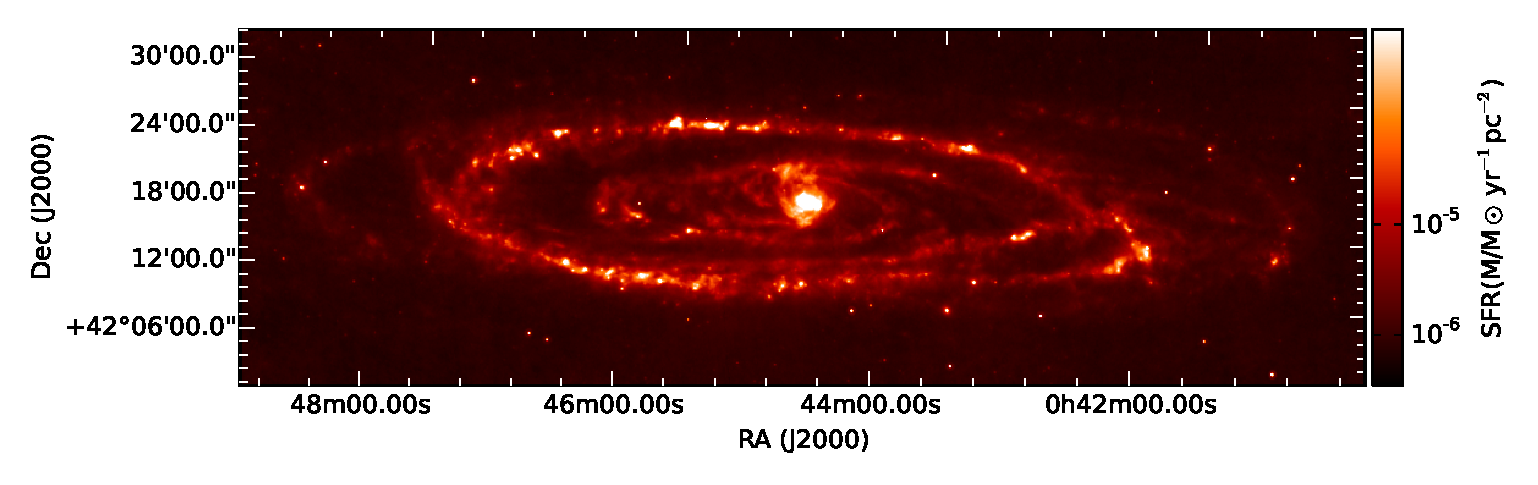
\includegraphics[width=164mm]{../image_paper1/sfr_fir.eps}
    \caption {SFR map calculated from total infrared emission (see Section~\ref{sec:sfr_fir}). The SFR map here has an angular resolution of 18\arcsec and pixel size of 9.85\arcsec, the same as the MIPS 70 $\mu$m map.}
    \label{fig:sfrs}
\end{figure*}

\subsubsection{\halpha plus 24 \um Star Formation Rate}
\label{sec:sfr_halpha}

The SFR can also be calculated using a combination of \halpha and \Spitzer  24 \um maps. \halpha emission of galaxies is dominated by light emitted from young and massive stars. Star formation timescales traced by this emission are $\sim 6-10$ Myr \citep[e.g.][]{Kennicutt09, Calzetti13}. Therefore, \halpha alone could be used to calibrate the SFR \citep[e.g.][]{Osterbrock06, Kennicutt09}. However, \halpha emission is very sensitive to dust extinction. Therefore, the combination of the \halpha and 24\um of considered a better choice for calculating the SFR. We used a calibration introduced by \citet{Kennicutt09} to measure the SFR:
\begin{equation}
\label{equ: halphaplus24_g}
SFR = 5.5 \times 10^{-42}[L(H{\alpha})_{\rm obs} + 0.020L(24\mu m)],
\end{equation}
\noindent where L(H${\alpha}$)$_{\rm obs}$ is the observed \halpha luminosity without correction for internal dust attenuation, given in the unit of erg~s$^{-1}$. L(24$\mu$m) is the $24\mu$m IR luminosity in erg~s$^{-1}$, and SFR is in M$_{\odot}~$yr$^{-1}$. It was indicated that the formulation above can only be used for the global situation, i.e., the total SFR.

\citet{Calzetti07} introduced a new calibration using the same bandpasses for the case of local regions:
\begin{equation}
\label{equ: halphaplus24_l}
SFR = 5.5 \times 10^{-42}[L(H{\alpha})_{obs} + 0.033L(24\mu m)],
\end{equation}
\noindent where the units here are the same as in equation~\ref{equ: halphaplus24_g}. Equation~\ref{equ: halphaplus24_l} is useful for regions less than $\sim 1$ kpc and is what we used for testing the SFR laws in local regions. The total M31 SFR calculated from summing pixel values and applying equation~\ref{equ: halphaplus24_g} is $0.35 \pm 0.01$~M$\sun$~yr$^{-1}$, which is in good agreement with previous studies.

\subsubsection{Total Infrared Star Formation Rate}
\label{sec:sfr_fir}
The total infrared emission of a system can also be used as a tracer of the SFR. Dust absorbs radiation from hot and young stars and re-emits it at infrared wavelengths; however, there is no one-to-one mapping between IR and UV emission. Therefore, integrating over the full wavelength range of the IR part and calculating the TIR luminosity is a better tracer of the SFR compared to IR single-band emission \citep{Calzetti13}. \citet{Calzetti13} assumed that stellar bolometric emission is completely absorbed and re-emitted by dust, i.e., $L_{star}(bol) = L(TIR)$, and calibrated the TIR luminosity of a system to calculate the SFR for a stellar population undergoing constant star formation over 100 Myr:
\begin{equation}
\label{equ:sfr_fir}
SFR(\rm TIR) = 2.8 \times10^{-44}L(\rm TIR),
\end{equation}
\noindent where SFR(TIR) and L(TIR), the star formation rate calculated from TIR emission and TIR luminosity, are in M$_{\odot}$~yr$^{-1}$ and erg~s$^{-1}$, respectively. Part of the dust emission in galaxies (specially in M31) comes from dust heated by the cosmic background radiation \citep[e.g.][]{Dole06, Calzetti13, Mattsson14}, hence, using equation~\ref{equ:sfr_fir} slightly overestimates the SFR in M31.  

Total infrared luminosity can be measured from the integration of the infrared part of a galaxy's spectral energy distribution or by combining photometric data at different IR wavelengths. As an example of the second approach, \citet{Draine07} modelled \Spitzer data and calibrated IR single-band photometry data to calculate the TIR luminosity. \citet{Boquien10} tested and modified this calibration as:
\begin{equation}
 \label{equ: TIR}
L(\rm TIR) = 0.95L(8) + 1.15L(24) + L(70) + L(160),
\end{equation}
\noindent where L(8), L(24), L(70), and L(160) are the luminosities of the galaxy at 8 $\mu$m, 24~$\mu$m, 70~$\mu$m, and 160~\um in units of erg~s$^{-1}$. We used results from equation~\ref{equ: TIR} in the equation~\ref{equ:sfr_fir} to calculate our final map of the M31 SFR (Figure~\ref{fig:sfrs}). Using this method, we calculated the total SFR by adding all the pixels to be $0.40 \pm 0.04$~M$_{\odot}$~yr$^{-1}$. Table~\ref{table:sfr} compares recent measurements of the total SFR of M31 from the literature and the present work. 


\begin{table*}
\begin{minipage}{100mm}
\caption{Comparison of the total star formation rate of M31}
\label{table:sfr}
\begin{tabular}{@{}lcc}
\hline\hline
Ref.&Method&SFR(M$_{\odot}$yr$^{-1}$) \\
\hline
Current work&FUV and 24~$\mu$m&0.31 \\
Current work&\halpha and 24~$\mu$m&0.35 \\
Current work&TIR luminosity&0.4\\
\citet{Ford13}&FUV and 24~$\mu$m&0.25\\
\citet{Ford13}&TIR luminosity&0.48-0.52\\
\citet{Azimlu11}& \halpha and 24~$\mu$m&0.34\\
\citet{Azimlu11}&Extinction-corrected \halpha&0.44\\
\citet{Tabatabaei10}&Extinction-corrected \halpha&0.27--0.38\\
\citet{Barmby06}&Infrared 8\um luminosity& 0.4\\
\hline
\end{tabular}
\end{minipage}
\end{table*}


%----------------------------------------------------------------------------------------
%ISM
%----------------------------------------------------------------------------------------


\subsection{Gas Surface Density}
\label{sec:ISM}

The molecular form of hydrogen is very difficult to detect. Therefore, CO (usually the $J(1\rightarrow 0)$ rotational transition, observed at 2.6 mm) is used as a tracer of the mass of the molecular cloud dominated by molecular hydrogen \citep[see, for example,][]{Sanders84}. Higher rotational transitions of CO can be used as tracers as well; however, they are not as common as $J(1\rightarrow 0)$. Equation~\ref{equ:conversion} shows the relation between CO emission and H$_2$ column density:
\begin{equation}
\label{equ:conversion}
\rm N_{H_2}/\rm cm^{-2} = X_{CO} \times I_{CO}/[{\rm K km s^{-1}}],
\end{equation}
\noindent where X$_{CO}$ is the conversion factor (also known as the X-factor), I$_{CO}$ is the CO intensity in  K~km~s$^{-1}$ and N$_{H_2}$ is the molecular hydrogen column density. The X-factor could be different in regions within a galaxy due to varying metallicity \citep{Wilson95, Bosselli02, Bolato13}. In the case of M31, different values of X-factor in the range of ($1-5.6 \times 10^{20}$) were adopted in previous studies \citep[e.g.][]{Ford13, Bolato13, Leroy11, Bolato08, Nieten06}; however, since any constant difference in X-factor leads to horizontal changes in a plot of log(SFR) versus log($\Sigma_{\rm {gas}}$) and does not affect our power-law indices for molecular gas, we chose $X_{\rm {CO}}= 2 \times 10^{20}$. This is the same value that is adopted in many other works \citep[e.g.][]{Ford13, Smith12}. Since H\,{\sc I} mass dominates over the H$_2$ mass in M31, the constant X-factor has a negligible effect on the total gas mass.

To calculate the mass of H$_2$ from the molecular hydrogen column density, we estimated the volume and volume density of H$_2$ in each pixel. Then, using M$_{H_2} = \mu_{H_2}m_H\rho_{H_2}$ where $ \mu_{H_2}$ is the mean molecular mass of H$_2$, m$_H$ is the mass of one hydrogen atom and $\rho_{H_2}$ is the volume density, we calculated M$_{H_2}$. 

The total gas mass was calculated from:
\begin{equation}
\label{equ:total_gas}
\rm M_{\rm \bld {total \, gas}} = 1.36[M_{\rm H I}+M_{H_2}],
\end{equation}
\noindent where the factor of 1.36 is a constant that takes into account the contribution of He and other heavier elements to the total gas mass, M$_{\rm H\,{\sc I}}$ is the mass of neutral hydrogen that was obtained from 21 cm observations (the map, which we got from \citet{Chemin09}, has units of number density which we used to calculate mass density of H\,{\sc I}), and M$_{H_2}$ was calculated from equation~\ref{equ:conversion} in units of M$_{\sun}$/pc$^2$. We assumed a gas mass of zero for regions where data for  either M$_{\rm H\,{\sc I}}$ or M$_{H_2}$ was not available, due to differences in coverage or bad pixels, etc. In this case the above equation gives a lower limit for the total gas; this applies to regions beyond 18~kpc from the galaxy centre.

%----------------------------------------------------------------------------------------
%STELLAR MASS
%----------------------------------------------------------------------------------------
\subsection{Stellar Mass}
\label{sec:starmass}
\begin{figure*}
\centering
\includegraphics[width=164mm]{../image_paper1/star.eps}.
\caption{The stellar mass surface density map produced using IRAC 3.6~$\mu$m data and the calibration presented in equation~\ref{equ:eskew}.}
\label{fig:stellarmass}
\end{figure*}

Emission in near-infrared bands, such as 3.6~$\mu$m, 4.5~\um and $K$-band, is almost insensitive to emission from young stellar populations, dust absorption and emission, which makes these bands good tracers of the mass of older stellar populations \citep[e.g.][]{Elmgreen84, Eskew12, Zhu10}.We calculated the stellar mass within M31 using a calibration of the 3.6 \um flux by \citet{Eskew12}. They used data from the Large Magellanic Cloud and introduced an empirical relation between stellar mass and flux:
\begin{equation}
\label{equ:eskew}
M _{\star}= 10^{5.97} F_{3.6}\left(\frac{D}{0.05}\right)^2,
\end{equation}
\noindent where M$_{\star}$ is the stellar mass in solar masses, $F_{3.6}$ is the 3.6~\um flux in Jy, and $D$ is the distance to the galaxy in Mpc. This calibration is based on the \citet{Salpeter55} IMF. Since the Kroupa IMF is adopted for the SFR maps, we corrected the calibration to the Kroupa IMF (see Section~\ref{sec: imf}). We should note that \citet{Eskew12} gave two calibrations for calculating the stellar mass in their paper: one is equation~\ref{equ:eskew} which only uses 3.6~\um emission and the other uses both 3.6~\um and 4.5~\um emission. We noticed that the second calibration can only be used in the case of total stellar mass due to the fact that the correlation shows a non-linear dependency of stellar mass on $F_{3.6 \mu m}$ and $F_{4.5 \mu m}$, though this was not mentioned in the aforementioned paper. 
Figure~\ref{fig:stellarmass} shows the stellar mass map for M31 using IRAC 3.6~\um in the original angular resolution and pixel size of the IRAC 3.6~\um image. Using the coverage map of the IRAC 3.6~\um data, we used only pixels with coverage of more than 2 images per sky position, and replaced the rest with zero M$_{\odot}$. The replaced pixels include less than 8\% of the data;  since these pixels are mainly  in regions with low surface brightness, their effect on the final total mass is less than 1\%.
Using this method we calculated the total stellar mass of the galaxy by adding all pixel values and found it to be $6.9 \times 10^{10}$M$_{\odot}$ $\pm$ 6\%. This result is in fairly good agreement with the results of \citet{Tamm12}. They calculate the stellar mass of M31 to be $(10-15) \times 10^{10}$M$_{\odot}$, 56\% of which is in the disk with the rest in the bulge of the galaxy. In their recent work on the stellar mass of M31, \cite{Viaene14} measured the total stellar mass using the integrated fluxes to be $5.49 \times 10^{10}$M$_{\odot}$, which is in good agreement with our result.



%----------------------------------------------------------------------------------------
%Metallicity
%----------------------------------------------------------------------------------------
\subsection{Metallicity}
\label{sec:metal}
 
The metallicity of a galaxy can be estimated by measuring abundances of heavier elements in its ISM. 
It is common to use  gas phase oxygen abundance, $[{\rm O/H}]$, as a gauge to determine metallicity \citep[e.g.][]{McGaugh91, Zaritsky94}. 
Results from modelling dust in the Milky Way and nearby galaxies showed that the dust to gas mass ratio depends on $[{\rm O/H}]$ and, consequently, on metallicity \citet{Draine07}. \citet{Draine14} assumed that depletion of gas elements from the gas to the diffuse ISM in M31 is similar to the Milky Way, and proposed that: 
 \begin{equation}
 \label{equ: metal}
\frac{M_d}{M_H}=0.0091 \frac{Z}{Z_{\odot}},
 \end{equation} 
\noindent where M$_d$ and M$_H$ are the total masses of dust and hydrogen, $Z$ is the metallicity of M31 and $Z_{\odot}$ is solar metallicity. 

\citet{Draine14} produced two dust maps of M31 using MIPS-160 resolution (FWHM  39\arcsec; 18\arcsec $\times$ 18\arcsec pixels) and SPIRE 350 resolution (FWHM 24\arcsec.9; 10\arcsec $\times$ 10\arcsec pixels), which are publicly available. 
We used the dust map with SPIRE 350 resolution, convolved and re-gridded  to have the same resolution and pixel size for the H\,{\sc I} map, then divided this dust mass by the mass of hydrogen in M31. 
However, in a private correspondence with the author, Draine pointed out that based on the Planck observations of Milky Way dust \citet{Tauber10}, the dust mass surface density map estimated for M31 by \citet{Draine14} may be systematically high by a factor of 2. We divided our dust map by 2 to account for this correction. 
We then generated a metallicity map of M31 by using the dust map in combination with equation~\ref{equ: metal}. \citet{Draine14} showed that with increasing distance from the centre of M31, the dust to H mass ratio declines monotonically and concluded that metallicity also behaves in the same way. 
Their fitting results showed that M31 can be divided into three regions ($R< 8~\kpc$, $8~\kpc < R < 18~\kpc$, and $18~\kpc < R \la 25~\kpc$) where the dust to H mass ratio (or metallicity) has a different correlation with galactocentric distance.
  
%----------------------------------------------------------------------------------------
%SFR LAWS
%----------------------------------------------------------------------------------------
\section{Scaling the star formation rate}
\subsection{Fitting method}
\label{sec:fitting}

%=164mm, height=218mm
\begin{figure*}
\centering
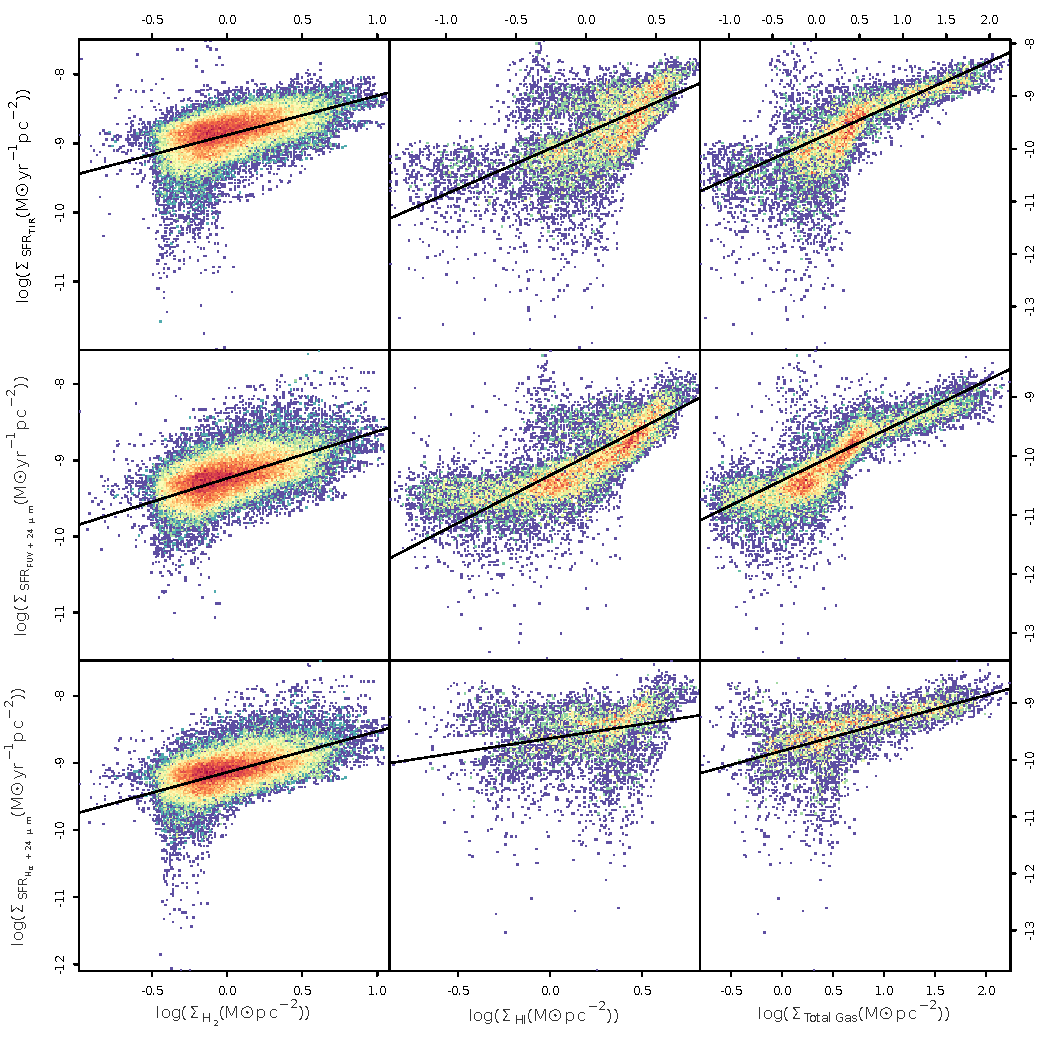
\includegraphics[width=\textwidth]{../image_paper1/ks_all_density.pdf}
\caption{Results from fitting the Kennicutt-Schmidt law to data from the whole galaxy using the pixel-by-pixel method. The colour represents the density of the pixels, increasing from blue to red. The number of points among the three columns is different due to the different angular resolution of the H\,{\sc I} and H$_2$ maps. Each point on the plots where the surface density of H$_2$ is used as a tracer of gas mass represents a region of size $\sim$30~pc (for maps with resolution of 23\arcsec) while each point for which the surface density of H\,{\sc I} or total gas mass is a tracer represents a region of size $\sim$155~pc (for maps with resolution of $60\arcsec \times 90\arcsec$). Solid lines show the best fit, using the mean value of the ranges in Table~\ref{table:res}.}
\label{fig:ks_all}
\end{figure*}

Producing the SFR, gas mass, stellar mass, and metallicity maps provides enough data to examine and compare the K-S law and the extended Schmidt law. To create surface density maps, we divided the value of each pixel by its area in pc$^2$. We investigated the K-S law and the extended Schmidt law using the pixel-by-pixel method in two ways. In one approach we used all the available pixels over the galaxy; in  the other approach we compare the laws in three elliptical regions at different distances from the centre of the galaxy as described in Section~\ref{sec:metal}, assuming a position angle of 38\degr and inclination of 77\degr\ for M31.
As mentioned in Section~\ref{sec: data_sfl}, since the H$_2$ gas mass map has higher angular resolution and smaller pixel size than the H\,{\sc I} gas mass map, our final results have two sets of different  angular resolutions and pixel sizes. 

Equations~\ref{equ:ks_org}~and~\ref{equ:es_org} can be re-written in logarithmic form to obtain two linear equations:
\begin{subequations}
\begin{equation}
\label{eq:sfr_law_ks_log}
\log_{10} \eqsigmasfr = N~\log_{10} \eqsigmagas + A,
\end{equation}
\begin{equation}
\label{eq:sfr_law_es_log}
\log_{10} \eqsigmasfr = \eqnprime~\log_{10} \eqsigmagas + \beta~\log_{10}\eqsigmastar  + A^\prime,
\end{equation}
\end{subequations}
\noindent where, {\it N}, $\eqnprime$, $\beta$, A, and A$^\prime$ are free fitting parameters. The units in the above equations are the same as those in equations~\ref{equ:ks_org} and ~\ref{equ:es_org}.

We found the free parameters by applying the hierarchical Bayesian linear regression method as described in \citet{Shetty13}. Shetty and colleagues used a Bayesian linear regression approach in a new method to find the K-S law parameters, considering the measurement uncertainties as well as hierarchical data structure.
We used the same technique as \citet{Shetty13} to estimate the K-S law parameters. For the extended Schmidt law, we extended the code such that instead of using  simple hierarchical Bayesian linear regression, which is used for the K-S law, it uses multiple hierarchical Bayesian linear regression. In this case, we were able to examine the effect of stellar mass on the SFR as shown in equation~\ref{eq:sfr_law_es_log}. 

Uncertainties in the SFR and stellar mass maps  were measured following the method described in \citet{Kennicutt07}. We used the quadratic sum of the variance of the local background for each luminosity map from the original pixel size images, Poisson noise of images, and calibration uncertainties. Note that this method measures the lower limit of the uncertainties for these variables. Uncertainties in H$_2$ mass were measured using the mean rms values of the  CO intensity, reported in \cite{Nieten06}. Uncertainties of the total gas map are calculated as the quadrature sum of the uncertainties in  H$_2$ and H\,{\sc I} masses. 

We also tested each law on three different regions which were chosen in the same manner as explained in Section~\ref{sec:metal}. Applying the SFR laws in these regions provides a tool to consider the effect of the distance from the centre of the galaxy on SFR laws such as metallicity, gas mass, stellar mass gradients and changing the ratio of H$_2$ to H\,{\sc I}. 


\subsection{Star formation laws}
\label{sec: sfl}

We made three SFR maps, three gas mass density maps and a stellar mass density map of the whole galaxy. We applied both laws on the whole galaxy using each combination of SFR and gas mass density tracer, along with applying the laws on three different regions. \citet{Kennicutt12} reviewed star formation in the Milky Way and nearby galaxies and described that there might be a breakdown of SFR laws for small size regions. Therefore, we re-gridded all the maps to have a pixel size equivalent to 750~pc, and repeated all of our processes on these new maps (Table~\ref{table:res750}). Additionally, we used these results to see if there is any correlation between the SFR laws and metallicity, as will be described in Section~\ref{sec:fittingmetal}.
 
\begin{figure*}

\includegraphics[width=168mm , height=230mm]{../image_paper1/Results_all_3_regs_after_err_co.pdf}
\caption{Same as figure~\ref{fig:ks_all}, but in this figure we separated pixels from different regions in the galaxy by their colours. The regions with $R< 8\kpc$, $8\kpc < R < 18\kpc$, and $18\kpc < R \la 25\kpc$ are shown in red, green and blue, respectively.}%%
\label{fig:ks,regs}
\end{figure*}


Figure~\ref{fig:ks_all} shows the pixel-by-pixel fitting of the K-S law on the whole galaxy. The first row of plots are the surface density of the SFR(TIR), which is calculated using the TIR emission from Section~\ref{sec:sfr_fir}, versus the gas surface density traced by only the molecular gas (H$_2$), only atomic gas (H\,{\sc I}), and total gas from right to left, respectively. 
The only difference between the upper and the other rows is that in the lower rows the SFR indicator is FUV plus 24~$\mu$m (second row), and \halpha plus 24~$\mu$m emission (third row). Figure~\ref{fig:ks,regs} shows the same data as Figure~\ref{fig:ks_all}. However, in this figure we separated pixels from different regions in the galaxy by their colours. 
 There is a deviation in the middle panel plots of Figure~\ref{fig:ks_all} which shows a set of points with with high star formation rate and low H\,{\sc I} gas.
As can be clearly seen in middle panel of Figure~\ref{fig:ks,regs}, this deviation is due to regions within 8~kpc of the centre of the galaxy (red points).
 \cite{Braun09} saw a similar feature in their studies of the K-S law in M31. 
The H\,{\sc I} surface density profile of M31 \citep[see figure 16 in][]{Chemin09} shows several local minima from the centre of M31 out to 30~kpc distance which could be a result of the H\,{\sc I} wrap. The H\,{\sc I} surface density map shows a lower density in the central regions compared to the ring area; on the other hand, the SFR maps show high densities in the central regions. The combination of the relatively low gas and high SFR causes the deviation. However,~~\cite{Braun09} argued that the high 24~$\mu$m fluxes in the centre of the galaxy are due to other processes such as shock heating rather than a large amount of star formation.
Since the total gas mass is calculated by adding H\,{\sc I} and H$_2$ gas mass, we can see this deviation in the right panel of Figure~\ref{fig:ks_all} as well. However, since we have H$_2$ emission in those regions these deviations are less prominent than the ones in the middle panel.

We took a similar approach for the extended Schmidt law. Figures~\ref{fig:es,all,fuv,tot}-~\ref{fig:es,regs,fuv,tot} and Figures~\ref{fig:es,all,fir,h2} - ~\ref{fig:es,all,halpha,tot} show the results of the pixel-by-pixel fitting of the extended Schmidt law. For the extended Schmidt law, we plotted our results in 3D to illustrate the relationship between the surface density of the SFR, the gas mass surface density, and stellar mass density more clearly. In this series of plots, the $x$-axis is the gas mass surface density, either molecular gas (H$_2$), atomic gas (H\,{\sc I}), or total gas, the $y$-axis is the SFR(TIR), SFR(FUV + 24~$\mu$m) or SFR(H$\alpha$ + 24~$\mu$m), and the $z$-axis is the stellar mass surface density. The shadows of the data on each surface are also plotted, to have a more clear picture of correlations between components. The shadows on the $x-y$ surface are the same as in Figure~\ref{fig:ks_all}. 

\begin{figure*}
        \centering
        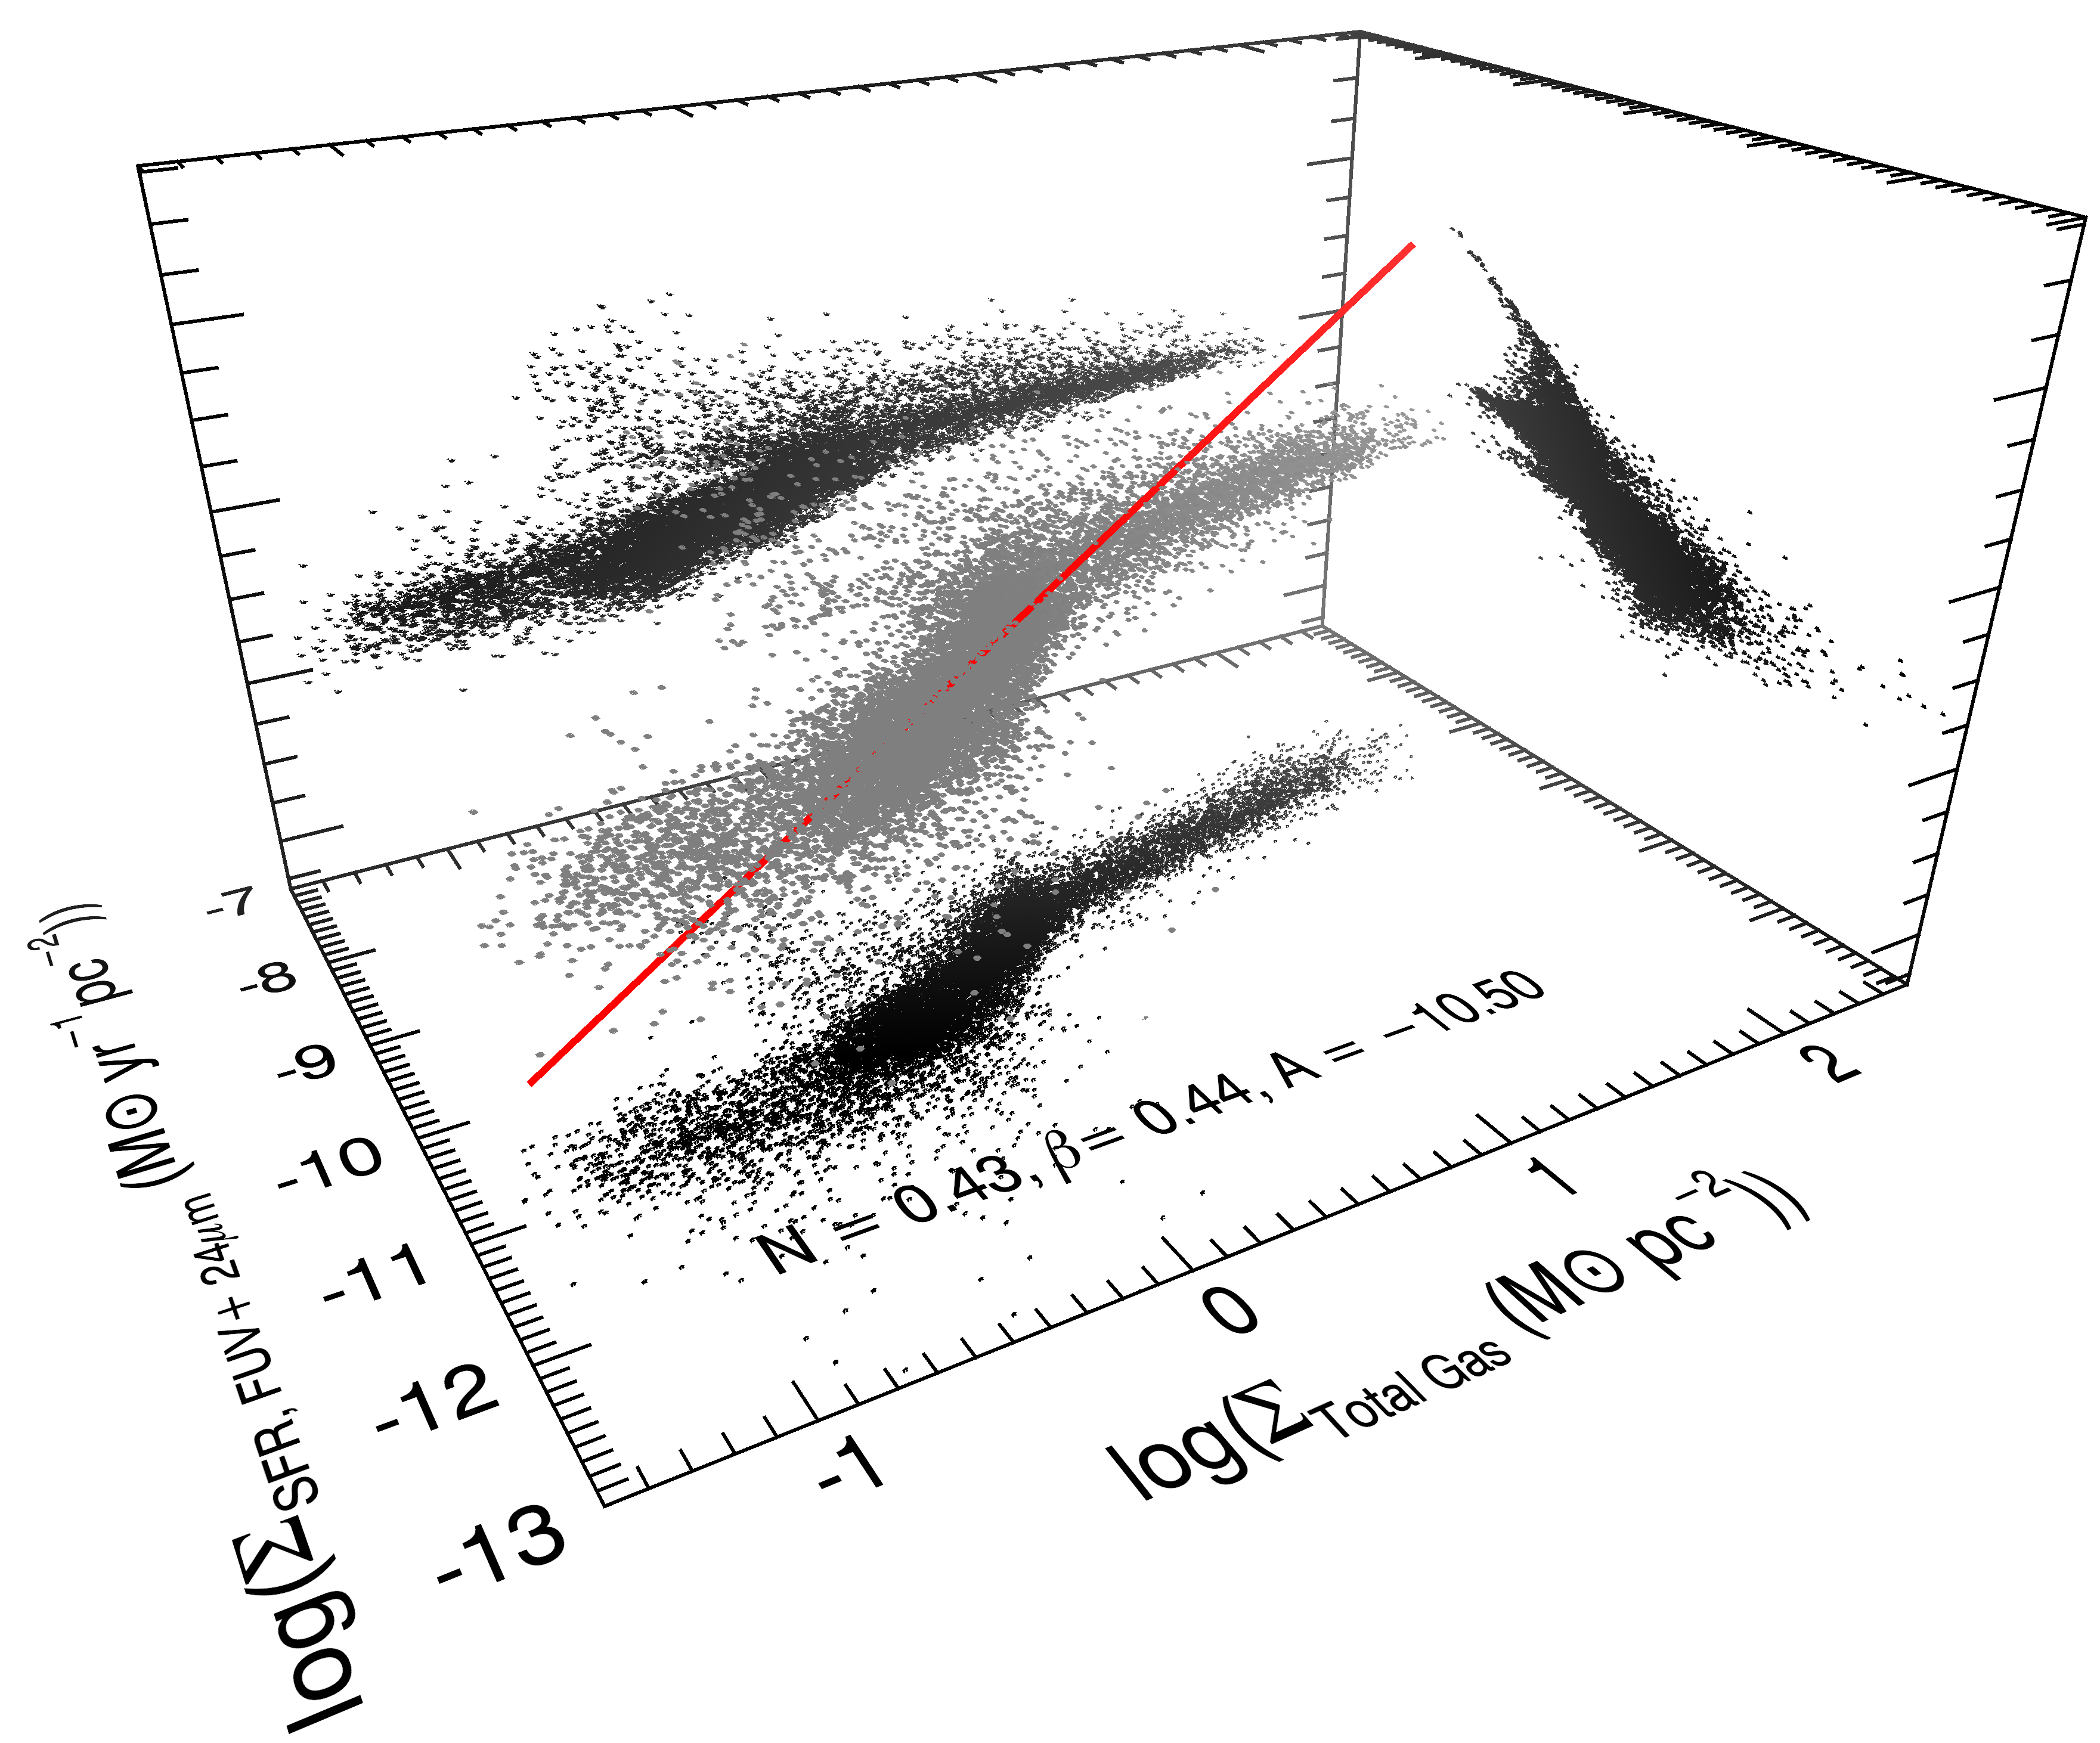
\includegraphics[width=\textwidth]{../image_paper1/es_tot_fuv_vs_tot2_f.png}
        \caption{The result from fitting the extended Schmidt law on the surface density of SFR(FUV + 24~$\mu$m), the surface density of total gas and the surface density of stellar mass ($z$-axis) from the whole galaxy. Solid line shows the best fit (the mean value of the range reported in Table~\ref{table:res}) from a pixel-by-pixel method. Equivalent plots for the other SFR and gas tracers are in Figures~\ref{fig:es,all,fir,h2} - ~\ref{fig:es,all,halpha,tot} in the appendix.}
        \label{fig:es,all,fuv,tot}
    \end{figure*}

\begin{figure*}
\centering
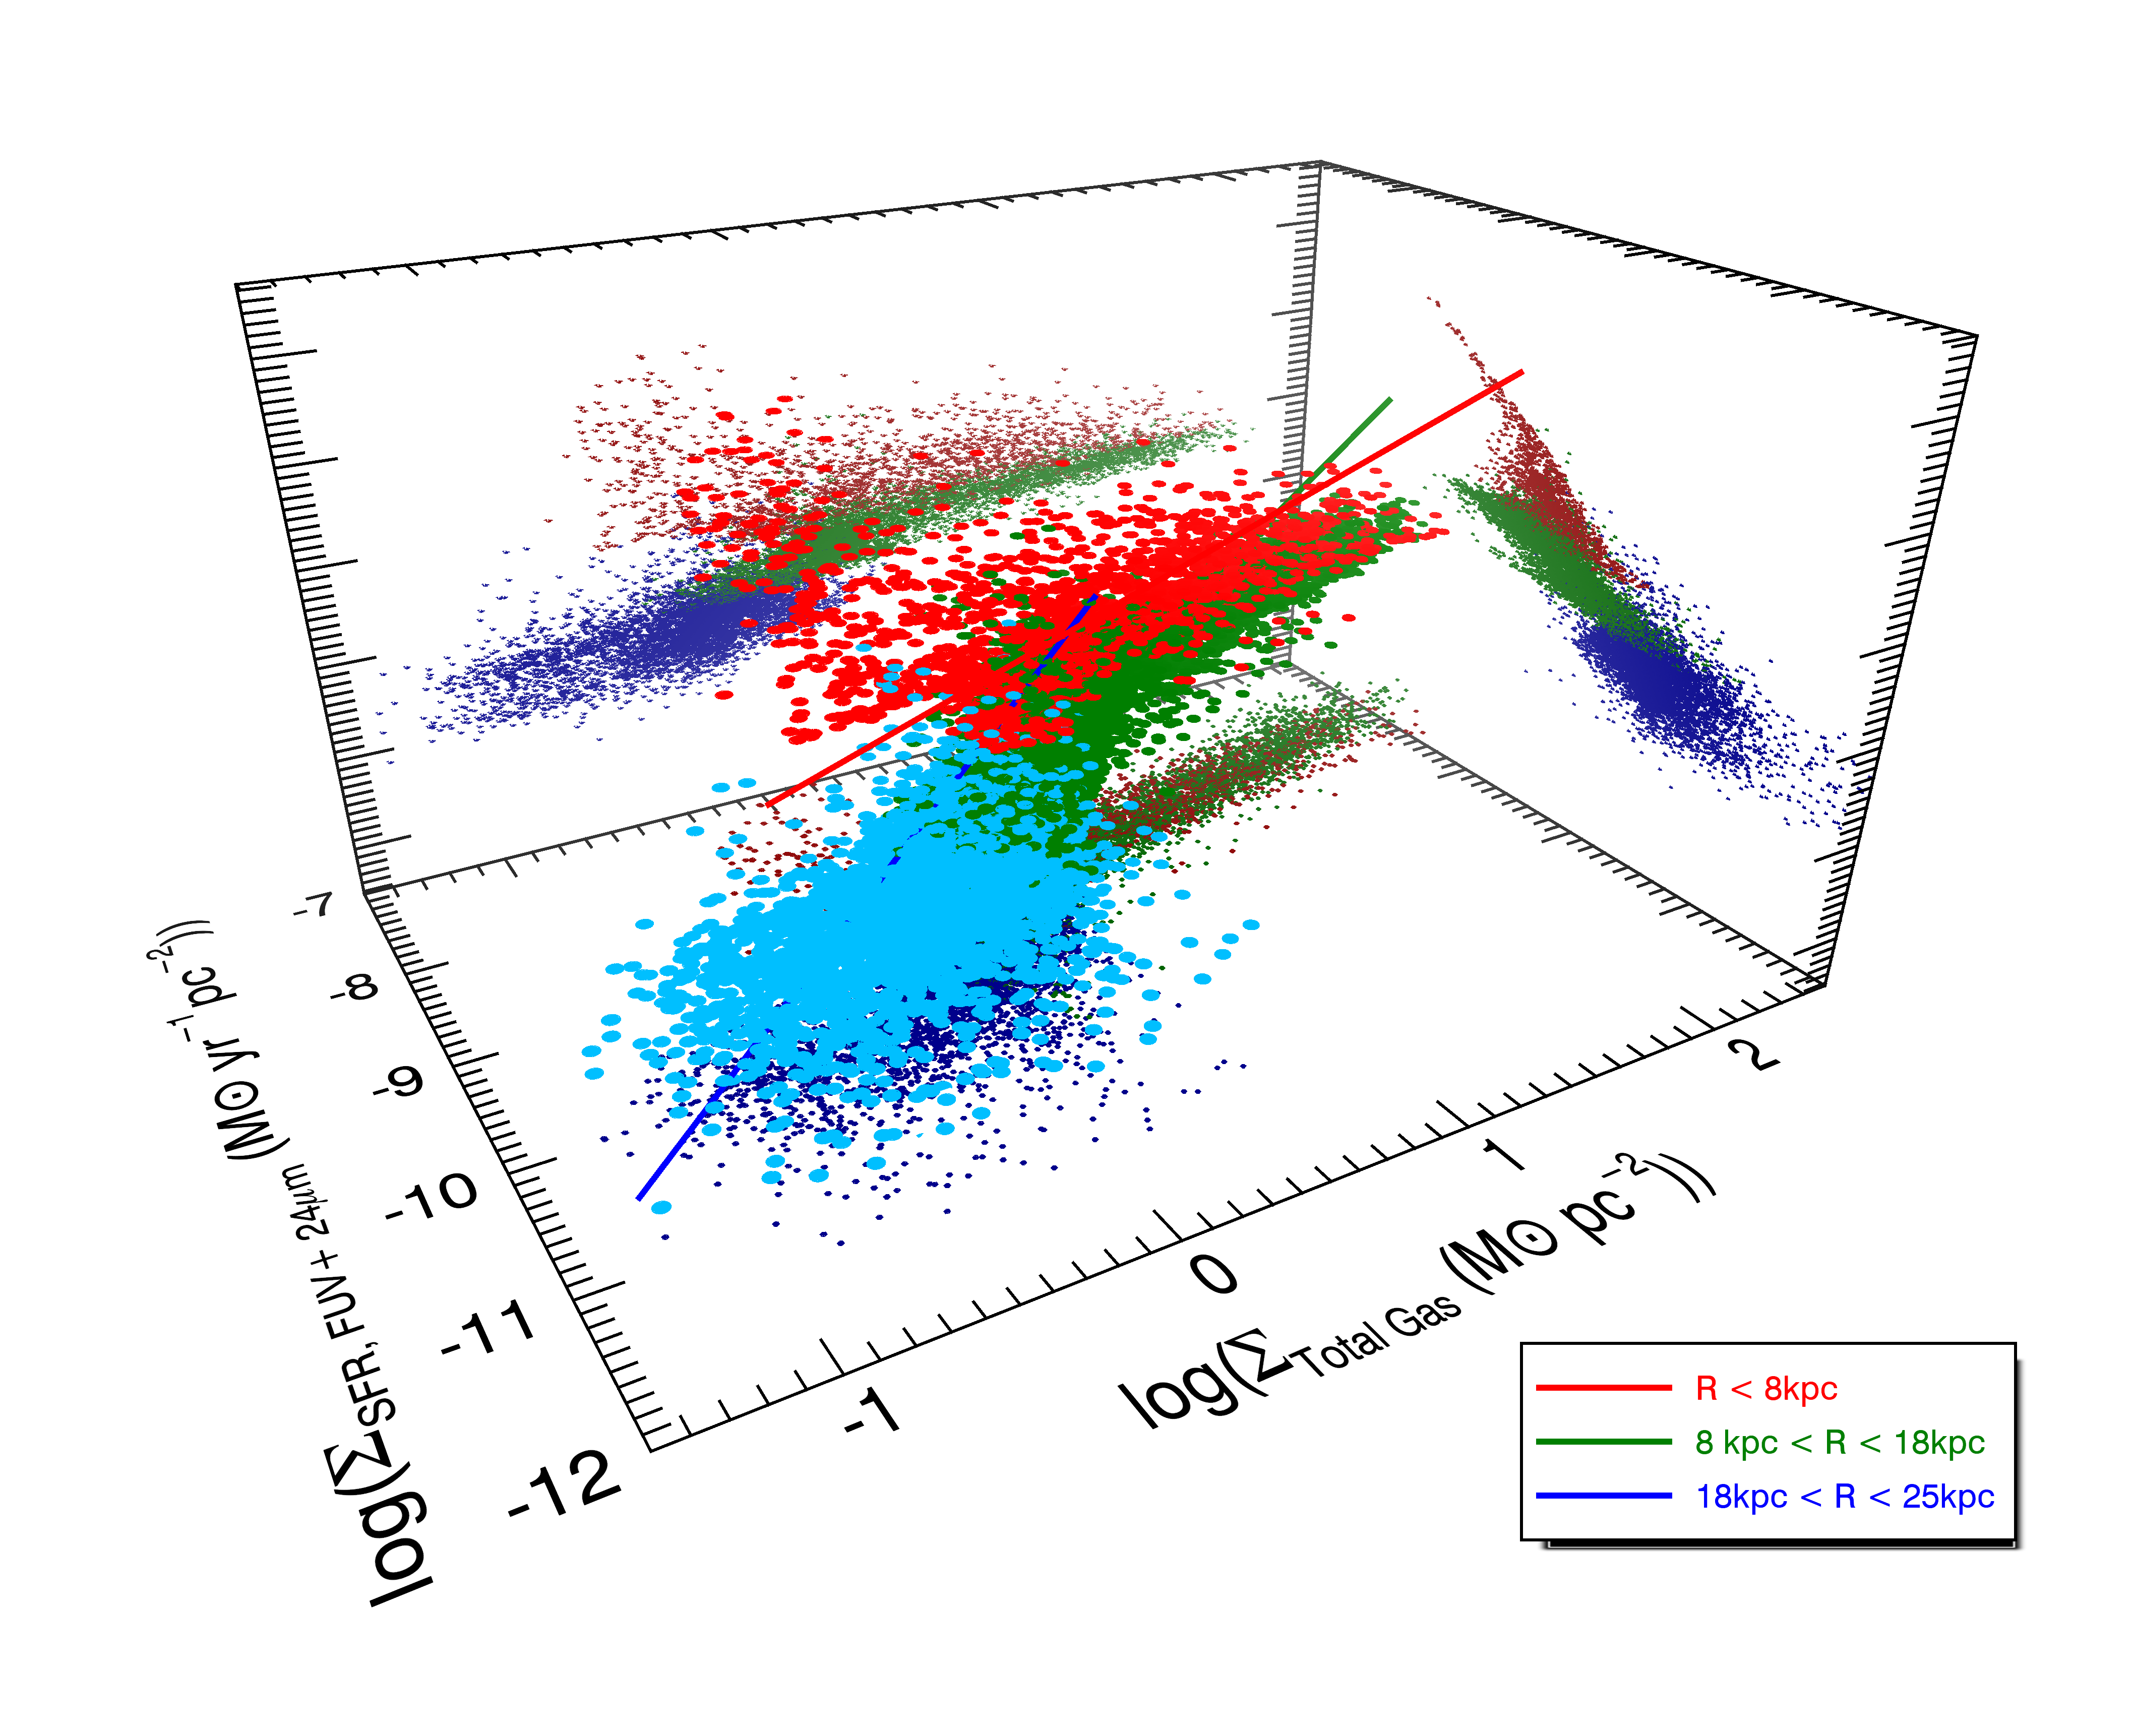
\includegraphics[width=\textwidth]{../image_paper1/color_3d_fuv_tot.png}
\caption{Fitting result for SFR(FUV + 24~$\mu$m) vs total gas. Same as Figure~\ref{fig:es,all,fuv,tot}, but in this figure we denote pixels from different regions in the galaxy by their colours. The regions with $R< 8\kpc$, $8\kpc < R < 18\kpc$, and $18\kpc < R \la 25\kpc$ are shown in red, green and blue, respectively.}
\label{fig:es,regs,fuv,tot}
\end{figure*}

\begin{figure*}
\centering
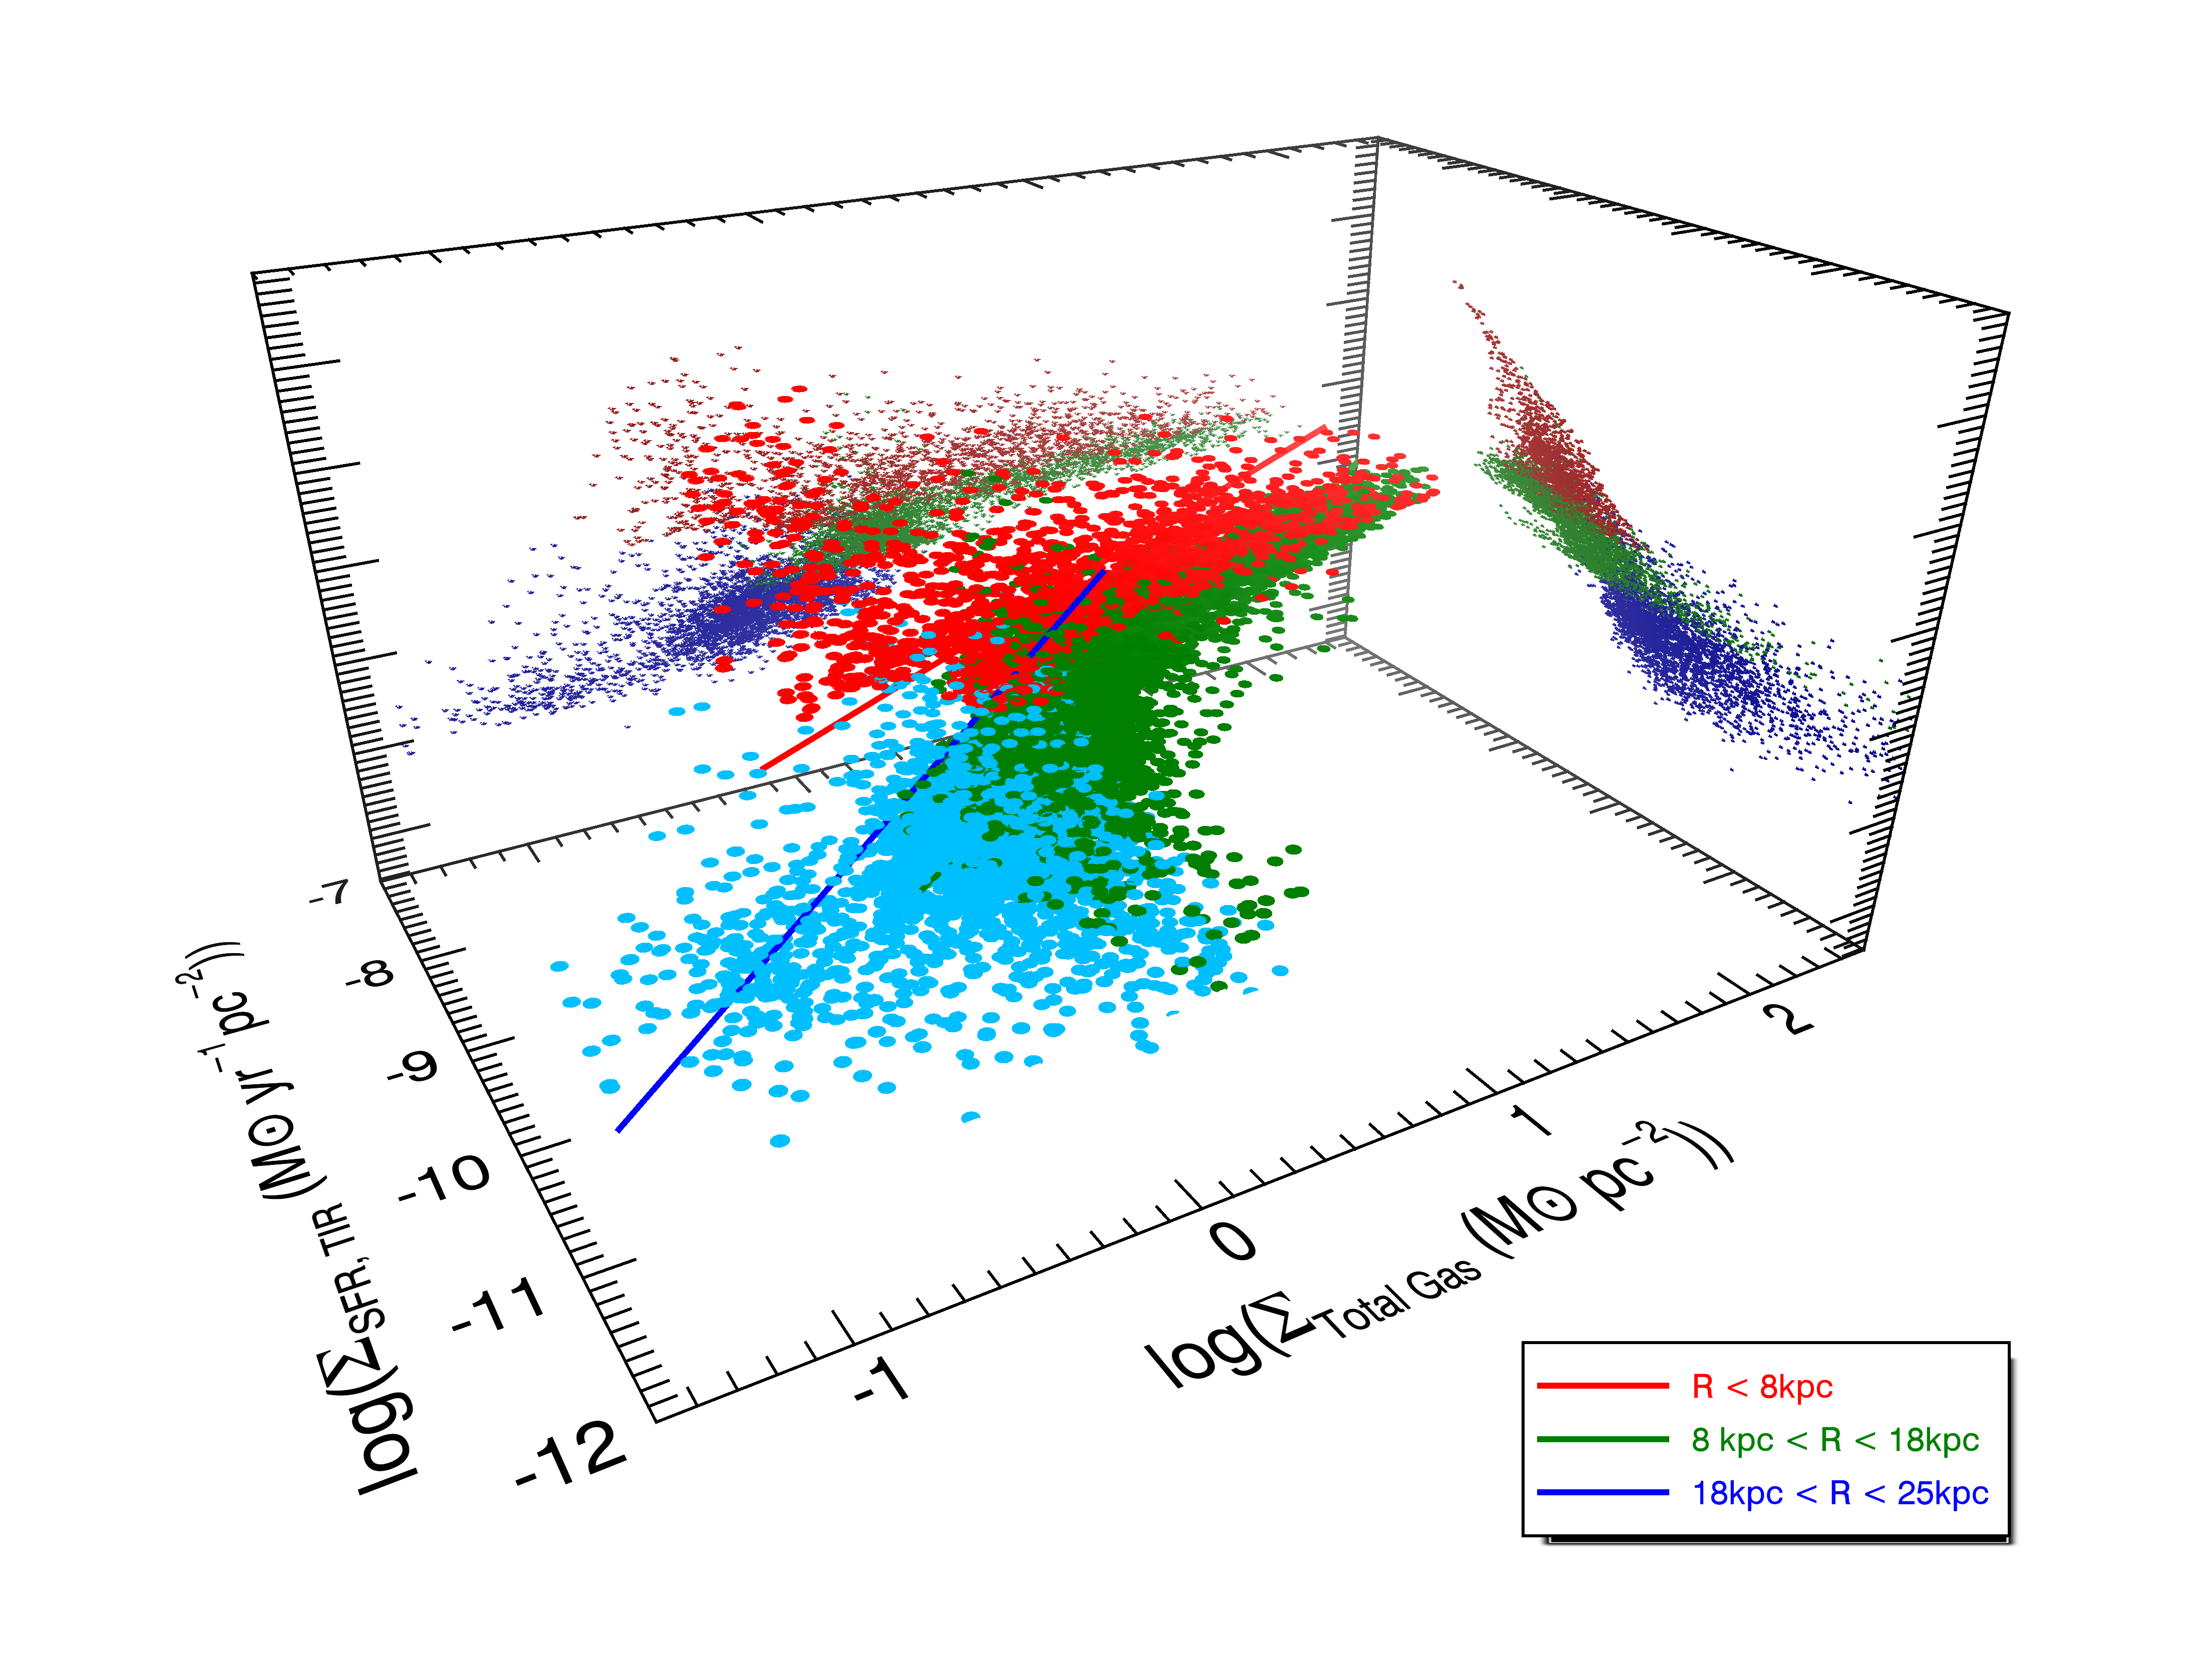
\includegraphics[width=\textwidth]{../image_paper1/color_3d_tir_tot.png}
\caption{Same as Figure~\ref{fig:es,regs,fuv,tot}, but in this figure we use total infrared emission as a tracer of the SFR.}
\label{fig:es,regs,fir,tot}
\end{figure*}

\begin{table*}
\caption{ K-S law and Extended Schmidt law fitting results}
\label{table:res}
\begin{tabular}{ccccccccc}
\hline\hline
\multicolumn{1}{c}{\multirow{1}{*}{Region}} & SFR Tracer & Gas Tracer & {\it N}    & A      & \nprime & $\beta$ & A$^\prime$ \\
\hline\hline
\multicolumn{1}{c}{\multirow{9}{*}{Whole Galaxy}} &TIR & H$_2$ only & 0.57 - 0.58 & -8.88 - -8.87  & 0.51 - 0.53  &  0.31 - 0.33 & -9.42 - -9.39  \\
& TIR               & HI only    & 1.13 - 1.19 & -9.71 - -9.69   & 0.76 - 0.79 & 0.74 - 0.75 & -10.58 - -10.56 \\
& TIR               & Total gas  & 0.73 - 0.75 & -9.85 - -9.84   & 0.46 - 0.48 & 0.53 - 0.55 & -10.40 - -10.38 \\
& FUV + 24\um       & H$_2$ only & 0.61 - 0.63 & -9.24 - -9.23   & 0.57 - 0.59 & 0.20 - 0.22 & -9.60 - -9.57   \\
& FUV + 24\um       & HI only    & 1.16 - 1.19 & -9.97 - -9.95   & 0.78 - 0.81 & 0.59 - 0.60 & -10.64 - -10.62 \\
& FUV + 24\um       & Total gas  & 0.67 - 0.70 & -10.10 - -10.09 & 0.42 - 0.44 & 0.43 - 0.45 & -10.51 - -10.49 \\
& H$\alpha$ + 24\um & H$_2$ only & 0.60 - 0.62 & -9.14 - -9.13   & 0.54 - 0.56  & 0.33 - 0.35  & -9.72 - -9.70 \\
& H$\alpha$ + 24\um & HI only    & 0.46 - 0.54 & -9.64 - 9.61    & 0.48 - 0.53 & 0.72 - 0.76 & -10.75 - -10.69 \\
& H$\alpha$ + 24\um & Total gas  & 0.48 - 0.51 & -9.85 - 9.82    & 0.32 - 0.35 & 0.54 - 0.58 & -10.59 - 10.54    \\
\hline
\multicolumn{1}{c}{\multirow{9}{*}{R$< 8\kpc$}} & TIR & H$_2$ only & 0.30 - 0.33  & -8.84 - -8.83 & 0.31 - 0.33 & 0.67 - 0.70 & -10.28 - -10.23  \\
 & TIR               & HI only    & 0.02 - 0.16  & -9.09 - -9.06 & 0.74 - 0.83 & 0.84 - 0.89 & -10.83 - -10.73 \\
 & TIR               & Total gas  & 0.20 - 0.24  & -9.22 - -9.18 & 0.28 - 0.30 & 0.70 - 0.73 & -10.70 - -10.63 \\
 & FUV + 24\um       & H$_2$ only & 0.37 - 0.41  & -9.22 - -9.21 & 0.26 - 0.32 & 0.43 - 0.46 & -10.01 - -9.96  \\
 & FUV + 24\um       & HI only    & -0.13 - 0.01 & -9.44 - -9.42 & 0.67 - 0.76 & 0.81 - 0.86 & -10.64 - -10.62 \\
 & FUV + 24\um       & Total gas  & 0.13 - 0.18  & -9.55 - -9.51 & 0.24 - 0.26 & 0.68 - 0.73 & -11.03 - -10.94 \\
 & H$\alpha$ + 24\um & H$_2$ only & 0.29 - 0.32  & -9.14 - -9.13 & 0.38 - 0.41 & 0.50 - 0.53 & -10.33 - -10.26  \\
 & H$\alpha$ + 24\um & HI only    & 0.00 - 0.10  & -9.26 - 9.24  & 0.48 - 0.53 & 0.61 - 0.64 & -10.51 - -10.44 \\
 & H$\alpha$ + 24\um & Total gas  & 0.13 - 0.16  & -9.34 - 9.32  & 0.18 - 0.19 & 0.50 - 0.53 & -10.41 - -10.35     \\
\hline
\multicolumn{1}{c}{\multirow{9}{*}{$8\kpc < $R $< 18\kpc$}} & TIR & H$_2$ only & 0.63 - 0.65 & -8.80 - -8.79   & 0.47 - 0.49 & 0.68 - 0.70 & -9.97 - -9.93   \\
 & TIR               & HI only    & 1.90 - 1.99 & -10.03 - -10.00 & 1.33 - 1.39 & 0.92 - 0.96 & -11.08 - -11.03 \\
 & TIR               & Total gas  & 0.76 - 0.79 & -9.89 - -9.87   & 0.55 - 0.58 & 0.53 - 0.58 & -10.70 - -10.63 \\
 & FUV + 24\um       & H$_2$ only & 0.66 - 0.68 & -9.16 - -9.15   & 0.54 - 0.56 & 0.54 - 0.57 & -10.12 - -10.08 \\
 & FUV + 24\um       & HI only    & 1.52 - 1.59 & -10.12 - -10.09 & 1.12 - 1.17 & 0.60 - 0.63 & -10.64 - -10.62 \\
 & FUV + 24\um       & Total gas  & 0.60 - 0.61 & -10.01 - -10.00 & 0.48 - 0.50 & 0.29 - 0.34 & -10.36 - -10.31 \\
 & H$\alpha$ + 24\um & H$_2$ only & 0.69 - 0.70 & -9.09 - -9.08   & 0.53 - 0.55 & 0.70 - 0.73 & -10.30 - 10.25  \\
 & H$\alpha$ + 24\um & HI only    & 1.28 - 1.35 & -10.00 - -9.95  & 0.64 - 0.76 & 1.17 - 1.26 & -10.51 - -10.44 \\
 & H$\alpha$ + 24\um & Total gas  & 0.62 - 0.65 & -10.04 - -10.01 & 0.39 - 0.43 & 0.75 - 0.85 & -11.04 - -10.91  \\
\hline
\multicolumn{1}{c}{\multirow{9}{*}{$18\kpc <$ R $\la 25\kpc$}} & TIR & H$_2$ only &  N/A$^a$ & N/A$^a$ & N/A$^a$ &N/A$^a$ & N/A$^a$ \\
 & TIR               & H\,{\sc I} only    & 0.44 - 0.54 & -9.96 - -9.94  & 0.33 - 0.41    & 0.31 - 0.36    & -10.22 - -10.18     \\
 & TIR               & Total gas  & 0.44 - 0.54 &  -10.00 - -9.98  & 0.33 - 0.41  & 0.31 - 0.36    & -10.25 -10.21     \\
 & FUV + 24~$\mu$m       & H$_2$ only & N/A$^a$ & N/A$^a$ & N/A$^a$ &N/A$^a$ & N/A$^a$    \\
 & FUV + 24~$\mu$m       & H\,{\sc I} only    & 0.65 - 0.72 & -10.18 - -10.16  & 0.59 - 0.67    & 0.17 - 0.22    & -10.33 - -10.29     \\
 & FUV + 24~$\mu$m       & Total gas  & 0.64 - 0.72 & -10.22 - -10.21  &  0.59 - 0.67   & 0.16 - 0.22    & -10.37 - -10.33     \\
 & H$\alpha$ + 24~$\mu$m & H$_2$ only &  N/A$^a$ & N/A$^a$ & N/A$^a$ &N/A$^a$ & N/A$^a$     \\
 & H$\alpha$ + 24~$\mu$m & H\,{\sc I} only    & 0.48 - 0.97 &  -9.97 - -9.88  & 0.61 - 1.12    & -0.36 - -0.12    & -9.82 - -9.59     \\
 & H$\alpha$ + 24~$\mu$m & Total gas  & 0.40 - 0.90 & -10.01 - -9.95  &  0.53 - 1.03    & -0.35 - -0.11    & -9.82 - -9.59     \\
 \hline
\end{tabular}
\begin{tablenotes}
 \item $^a$  Since there are very few pixels which we can use for the fitting in this region we cannot provide a meaningful result.
\item Each entry shows the 95\% confidence range for the fitting parameter.
\item Fitting parameters of SF laws from applying the Bayesian method.  {\it N} is the power-law index of the K-S law; A is the intercept of the K-S law; \nprime is the gas power-law index in the extended Schmidt law;
 $\beta$ is the power-law index of the stellar component in the extended Schmidt law; and A$^\prime$ is the intercept of the extended Schmidt law.
\end{tablenotes}
\end{table*}








\begin{table*}
\caption{K-S law and Extended Schmidt Law fits for larger pixels}
\label{table:res750}
\begin{tabular}{cccccccc}
\hline\hline
\multicolumn{1}{c}{\multirow{1}{*}{Region}}  & Gas Tracer & {\it N} & A  & \nprime & $\beta$ & A$^\prime$ \\
\hline\hline
\multicolumn{1}{c}{\multirow{3}{*}{Whole Galaxy}}
 & H$_2$ only & 0.26 - 0.31 & -10.00 - -9.91  & 0.21 - 0.26  & 0.26 - 0.40    & -10.51 - -10.30  \\
 & H\,{\sc I} only    & 1.08 - 1.24 & -11.60 - -11.36  & 0.73 - 0.85  & 0.58 - 0.64    & -11.74 - -11.60     \\
 & Total gas  & 0.66 - 0.73 & -10.11 - -10.06 & 0.39 - 0.46    & 0.41 - 0.49    & -11.56 - -10.47     \\
\hline
\multicolumn{1}{c}{\multirow{3}{*}{R$< 8\kpc$}}
 & H$_2$ only & 0.14 - 0.27 & -9.82 - -9.59  & 0.14 - 0.21   & 0.48 - 0.66   & -11.04 - -10.66      \\
 & H\,{\sc I} only    & 1.42 - 1.68 & -12.35 - -11.92 & 0.51 - 0.92    & 0.72 - 0.97    & -12.52 - -11.61     \\
 & Total gas  & 0.07 - 0.31 & -9.63 - -9.45  & 0.22 - 0.32    & 0.63 - 0.78    & -11.17 - -10.84      \\
\hline
\multicolumn{1}{c}{\multirow{3}{*}{$8\kpc < $R $< 18\kpc$}}
 & H$_2$ only & 0.27 - 0.32 & -9.98 - -9.86  & 0.17 - 0.24    &  0.38 - 0.73   & -10.89 - -10.44       \\
 & H\,{\sc I} only    & 0.88 - 1.38 & -11.80 - -11.06 & 1.00 - 1.22    & 0.53 - 0.69    & -12.41 - -12.09     \\
 & Total gas  & 0.55 - 0.64 & -10.03 - -9.96 & 0.40 - 0.51    & 0.27 - 0.49    & -10.53 - -10.29     \\
\hline
\multicolumn{1}{c}{\multirow{3}{*}{$18\kpc <$ R $\la 25\kpc$}} 
 & H$_2$ only & N/A$^a$& N/A$^a$ & N/A$^a$ &N/A$^a$ & N/A$^a$    \\
 & H\,{\sc I} only    & 0.46 - 0.81 & -11.21 - -10.80  & 0.44 - 0.76    & 0.13 - 0.36    & -11.35 -10.94     \\
 & Total gas  & 0.47 - 0.82 & -10.25 - -10.18 & 0.44 - 0.78    & 0.12 - 0.36    & -10.49 - -10.30     \\
 \hline
\end{tabular}
\begin{tablenotes}
\item Similar to Table~\ref{table:res} but here the fitting is performed on regions with a size of 750~pc, and we only show the results from SFR(FUV+24$\mu$m).
\end{tablenotes}
\end{table*}



%----------------------------------------------------------------------------------------
%
%----------------------------------------------------------------------------------------
\section{Discussion}

Table~\ref{table:res} shows the results of the hierarchical Bayesian fitting for the whole galaxy and all three regions. Considering the data and uncertainties for each parameter, we are 95\% confident that our fitting parameter is in the ranges given in Table~\ref{table:res}.
Our results suggest that changing the gas tracer has a more significant impact on the determination of the power law index than changing the SFR tracers. Therefore, we only discuss the results from SFR(FUV+24$\mu$m), and in Table~\ref{table:res750} we only show results from this SFR map.

\subsection{The K-S law in M31}

As mentioned before, the K-S law in M31 has been tested by many groups. In one of the most recent works on M31, \citet{Ford13} investigated the K-S law in six annuli and the global case using the ordinary least squares fitting method. 
To make a meaningful comparison between our results and the results reported in \citet{Ford13}, we averaged the power-law indices in \citet{Ford13} with a certain annuli and compared to the results with the same annuli in ours. We calculated power-law indices to be in the case of the H$_{2}$-only gas $N \sim 0.35, 0.58, 0.68$ and in case of total gas, $N \sim 1.37, 2.05, 1.60$ for $R< 8\kpc$, $8\kpc < R < 18\kpc$, and $18\kpc < R \la 25\kpc$, respectively.
\citet{Tabatabaei10} also applied the K-S law to M31 using the OLS fitting method, and have some differences with results from \citet{Ford13}. \citet{Ford13} argued that the main reason for these differences is the cut-off they used to fit the data. 
 
The whole-galaxy fit of the K-S law shows that using total gas or H$_{2}$-only gas gives a sub-linear relation between \sigmasfr and \sigmatotalgas. When using  H\,{\sc I}-only gas we find a nearly super-linear relation. These results are different from the power-law index estimated by \citet{Ford13}  in the case of total gas, $N=2.03\pm0.04$, but similar to their value of $N=0.6\pm0.01$ in the case of H$_{2}$-only gas. 
\citet{Tabatabaei10} estimated the K-S law power index as $N=1.30\pm0.05$ using total gas and $N=0.96\pm0.03$ using H$_{2}$-only gas. The reason behind these differences is mostly because of the statistical method we chose. The OLS fitting using H$_{2}$-only gas gives us a power-law index of $N=0.54\pm0.003$ which is close to the \citet{Ford13} results but still different fro \citet{Tabatabaei10}, perhaps for the same reason \citet{Ford13} suggested for the discrepancy between their results and results from \citet{Tabatabaei10}. We also noticed that different methods of measuring the uncertainties affect the power-law indexes, as well. The OLS fitting with \sigmatotalgas gives $N=0.74\pm0.003$, which is still lower than values in both  \citet{Tabatabaei10} and  \citet{Ford13}. Different methods in making the total gas map and using different criteria to choose outliers are the main reasons for this difference.

 \citet{Bigiel08} argued that there is no universal relationship between the surface density of the total gas and the SFR. They also showed that the SFR and the molecular hydrogen have a linear relationship. \citet{Shetty13} used the same data as \citet{Bigiel08} and argued that using the hierarchical Bayesian fitting leads to significant galaxy-by-galaxy variation between power-law indices with all of them being lower than those of \citet{Bigiel08}. Although some of our results in Table~\ref{table:res} showed a nearly linear correlation, we did not find any specific trend between power-law indices in the different regions.

The sub-linear power-law index in the case of the total gas or molecular gas surface density suggests that the star formation efficiency is decreasing as the total gas increases. Consequently, the depletion time increases. On the contrary, the super-linear relation suggests that the depletion time is decreasing with an increasing amount of H\,{\sc I} gas. The latter conclusion is more similar to the initial suggestion of the K-S law. If we assume that stars form in the molecular clouds, decreasing SFE with increasing total gas is justifiable.

The hierarchical Bayesian fitting on the $8<R<18$~kpc region gives similar values as the fitting to the whole galaxy data. This region contains the 10~kpc ring, which is where most of the star formation is happening, so it dominates the results from the whole galaxy.  For the other two regions, the K-S law fitting gives a sub-linear relation between the SFR and the gas surface density. A sub-linear relationship between \sigmasfr and  $\Sigma_{H_2}$ indicates that there are some CO-bright regions which do not associate with star forming regions.
 \citet{Krumholz09} showed that for regions with \sigmagas~$\leq 100$~M$_{\odot}$~pc$^{-2}$, \sigmasfr and $\Sigma_{H_2}$ have a nearly linear correlation. They also conclude that, at intermediate total gas column density, (\sigmagas~$\leq 100$~M$_{\odot}$~pc$^{-2}$), \sigmasfr and \sigmagas have a linear or slightly sub-linear correlation. The latter conclusion agrees with our results.


The K-S law power-law index varies with the distance to the centre of the galaxy. Similar to results from \citet{Ford13}, the power-law index considering molecular gas only increases with increasing distance from the centre of the galaxy. The power-law index using total gas or atomic gas does not show any particular correlation with distance. The increase of the power-law index while using molecular cloud only may be an effect of the decreasing metallicity across the galaxy or other physical properties of the galaxy such as stellar mass (see Section~\ref{sec:es_res}).
  
\subsection{The extended Schmidt law in M31}
\label{sec:es_res}
The extended Schmidt law has been a recently proposed law \citep{Shi11}, which shows a tight correlation between the SFR and the total gas surface density and the surface density of the stellar mass. Our results from fitting the whole galaxy shows a sub-linear relation between \sigmasfr and \sigmastar.
Using only atomic gas, $\beta$ is in good agreement with the original suggestion of the extended Schmidt law, $\eqnprime = 0.8 \pm 0.01$ and $\beta = 0.62\pm0.01$. However, $\beta$ is much smaller in other two gas tracers. Using total gas mass, we find $\eqnprime$ to be very close to $\beta$. This relation suggests that, although increasing the total gas causes a decrease to the SFE, the existing stars will increase the SFE. 

The fitting result on the $8<R<18$~kpc region (see Table~\ref{table:res}) is similar to that from fitting the whole galaxy together.  Taking the average $\beta$ from the atomic gas only fits gives us $\eqnprime \sim 0.79$ which is in good agreement with \citet{Shi11}, but $\beta = 0.53$  which is smaller than the original suggestion of the extended Schmidt law. However, the final indices reported by \citet{Shi11} for  the extended Schmidt law are an average over 12 different spiral galaxies, and some of their individual galaxies (e.g. NGC 4736, NGC 4726) have similar values as for M31.
Similar to the K-S law, the extended Schmidt law results are sensitive to the fitting method. Using the OLS fitting, one only will consider the SFR and stellar mass surface density errors, nevertheless, the hierarchical Bayesian regression fitting considers uncertainties on all the parameters.
 

Thus we can conclude that the SFR is higher in regions with higher stellar mass surface density than those with less stellar mass surface density.
In most cases this effect is almost as strong as the effect of gas surface density on the SFR.
\citet{Kim13}, using 3D numerical hydrodynamic simulations, showed that in the outer disk regions of a galaxy where the total gas is dominated by H\,{\sc I} gas, the SFR correlates with $\rho_{sd}^{0.5}$ where $\rho_{sd}$ is the mid-plane density of the stellar disk plus dark matter. This is because in the outer regions of the disk, the gravity from stars dominates. 
We calculated the power index related to the stellar mass surface density to be 0.36 for these regions (Table~\ref{table:res750}) which is slightly different from their suggestion. Since we do not have enough H$_2$ data for regions within $18\kpc < R \la 25\kpc$, our results are limited to ones from the extended Schmidt law for H\,{\sc I} gas only. Therefore, we could neither confirm nor refuse this prediction.

\subsection{Metallicity}
\label{sec:fittingmetal}
It is well established that the metallicity of M31 is higher in the centre than it is in the outer disk  \citep[e.g.][]{Draine14}. The inverse correlation between metallicity and the X-factor, which was described in Section~\ref{sec: intro_sfl}, leads to an underestimation of the power-law indices from fitting the K-S law in the case of the molecular gas only and total gas. 
Thus a corrected power-law index of the K-S law is higher than shown in Table~\ref{table:res}. Another correlation between components of the SFR laws and metallicity was introduced by \citet{Krumholz09}. 
They found a new SFR law based on a correlation between SFR and metallicity, and suggested that this correlation strongly depends on the amount of total gas in galaxies. They also showed the SFR has a dependence on metallicity which we saw a weak correlation (Figure~\ref{fig:metal}).
 We estimated the SFR using \citet{Krumholz09} SFR laws for regions with size of $\sim$750~pc.
Using the mid value of metallicity, 1.65, and clumping factor of 1.2, We found that the SFR calculated using the Krumholz law is, on average, different by 45\% from the measured SFR(FUV + 24~$\mu$m) in this work. 

In more recent studies, \citet{Mannucci10} and \citet{Lilly13} assumed the K-S law holds for their sample of local and high-redshift galaxies and obtained a correlation between metallicity and the stellar mass, the gas mass and the SFR. 
They found that increasing both the SFR and the stellar mass increases metallicity, but increasing the gas mass decreases metallicity (equation 9 in \citep{Mannucci10}). 
However, by considering results from \citet{wong13} regarding the dependence of the rate of H\,{\sc I}-H$_2$ conversion to metallicity, \citet{Roychowdhury15} showed that the K-S law is independent of metallicity in galaxies with H\,{\sc I} as a dominant gas. 

In Figure~\ref{fig:metal}, we plot dust to gas mass ratio versus the SFR(FUV + 24~$\mu$m) and the stellar mass, and could not find any correlation over the scale of the whole galaxy.
We calculated the Pearson correlation coefficients between metallicity and SFR, and between metallicity and the stellar mass, and found them to be 0.08 and 0.04, respectively. 
However, in Figure~\ref{fig:metal}, we can see a correlation between metallicity and both SFR and stellar mass for regions within $R< 18\kpc$. These are weak correlations with Pearson correlation coefficients of $-0.58$ and $-0.46$ for the SFR case and the stellar mass case, respectively.
We cannot see any correlation in the data from $18\kpc < R \la 25\kpc$. The average metallicity uncertainty in this region is almost 10 times higher than the average uncertainty for the rest of the galaxy. This higher uncertainty obscures any tentative correlation between metallicity and SFR or stellar mass for from $18\kpc < R \la 25\kpc$.   
This analysis confirms that there is a correlation between metallicity and both the SFR/the stellar mass. Although we could not find any strong correlation between the SFR and metallicity, especially in outer disk regions, we should note that the effect of the metallicity on SF laws is ambiguous and more high resolution data is needed to solve this puzzle.

\begin{figure*}
\centering
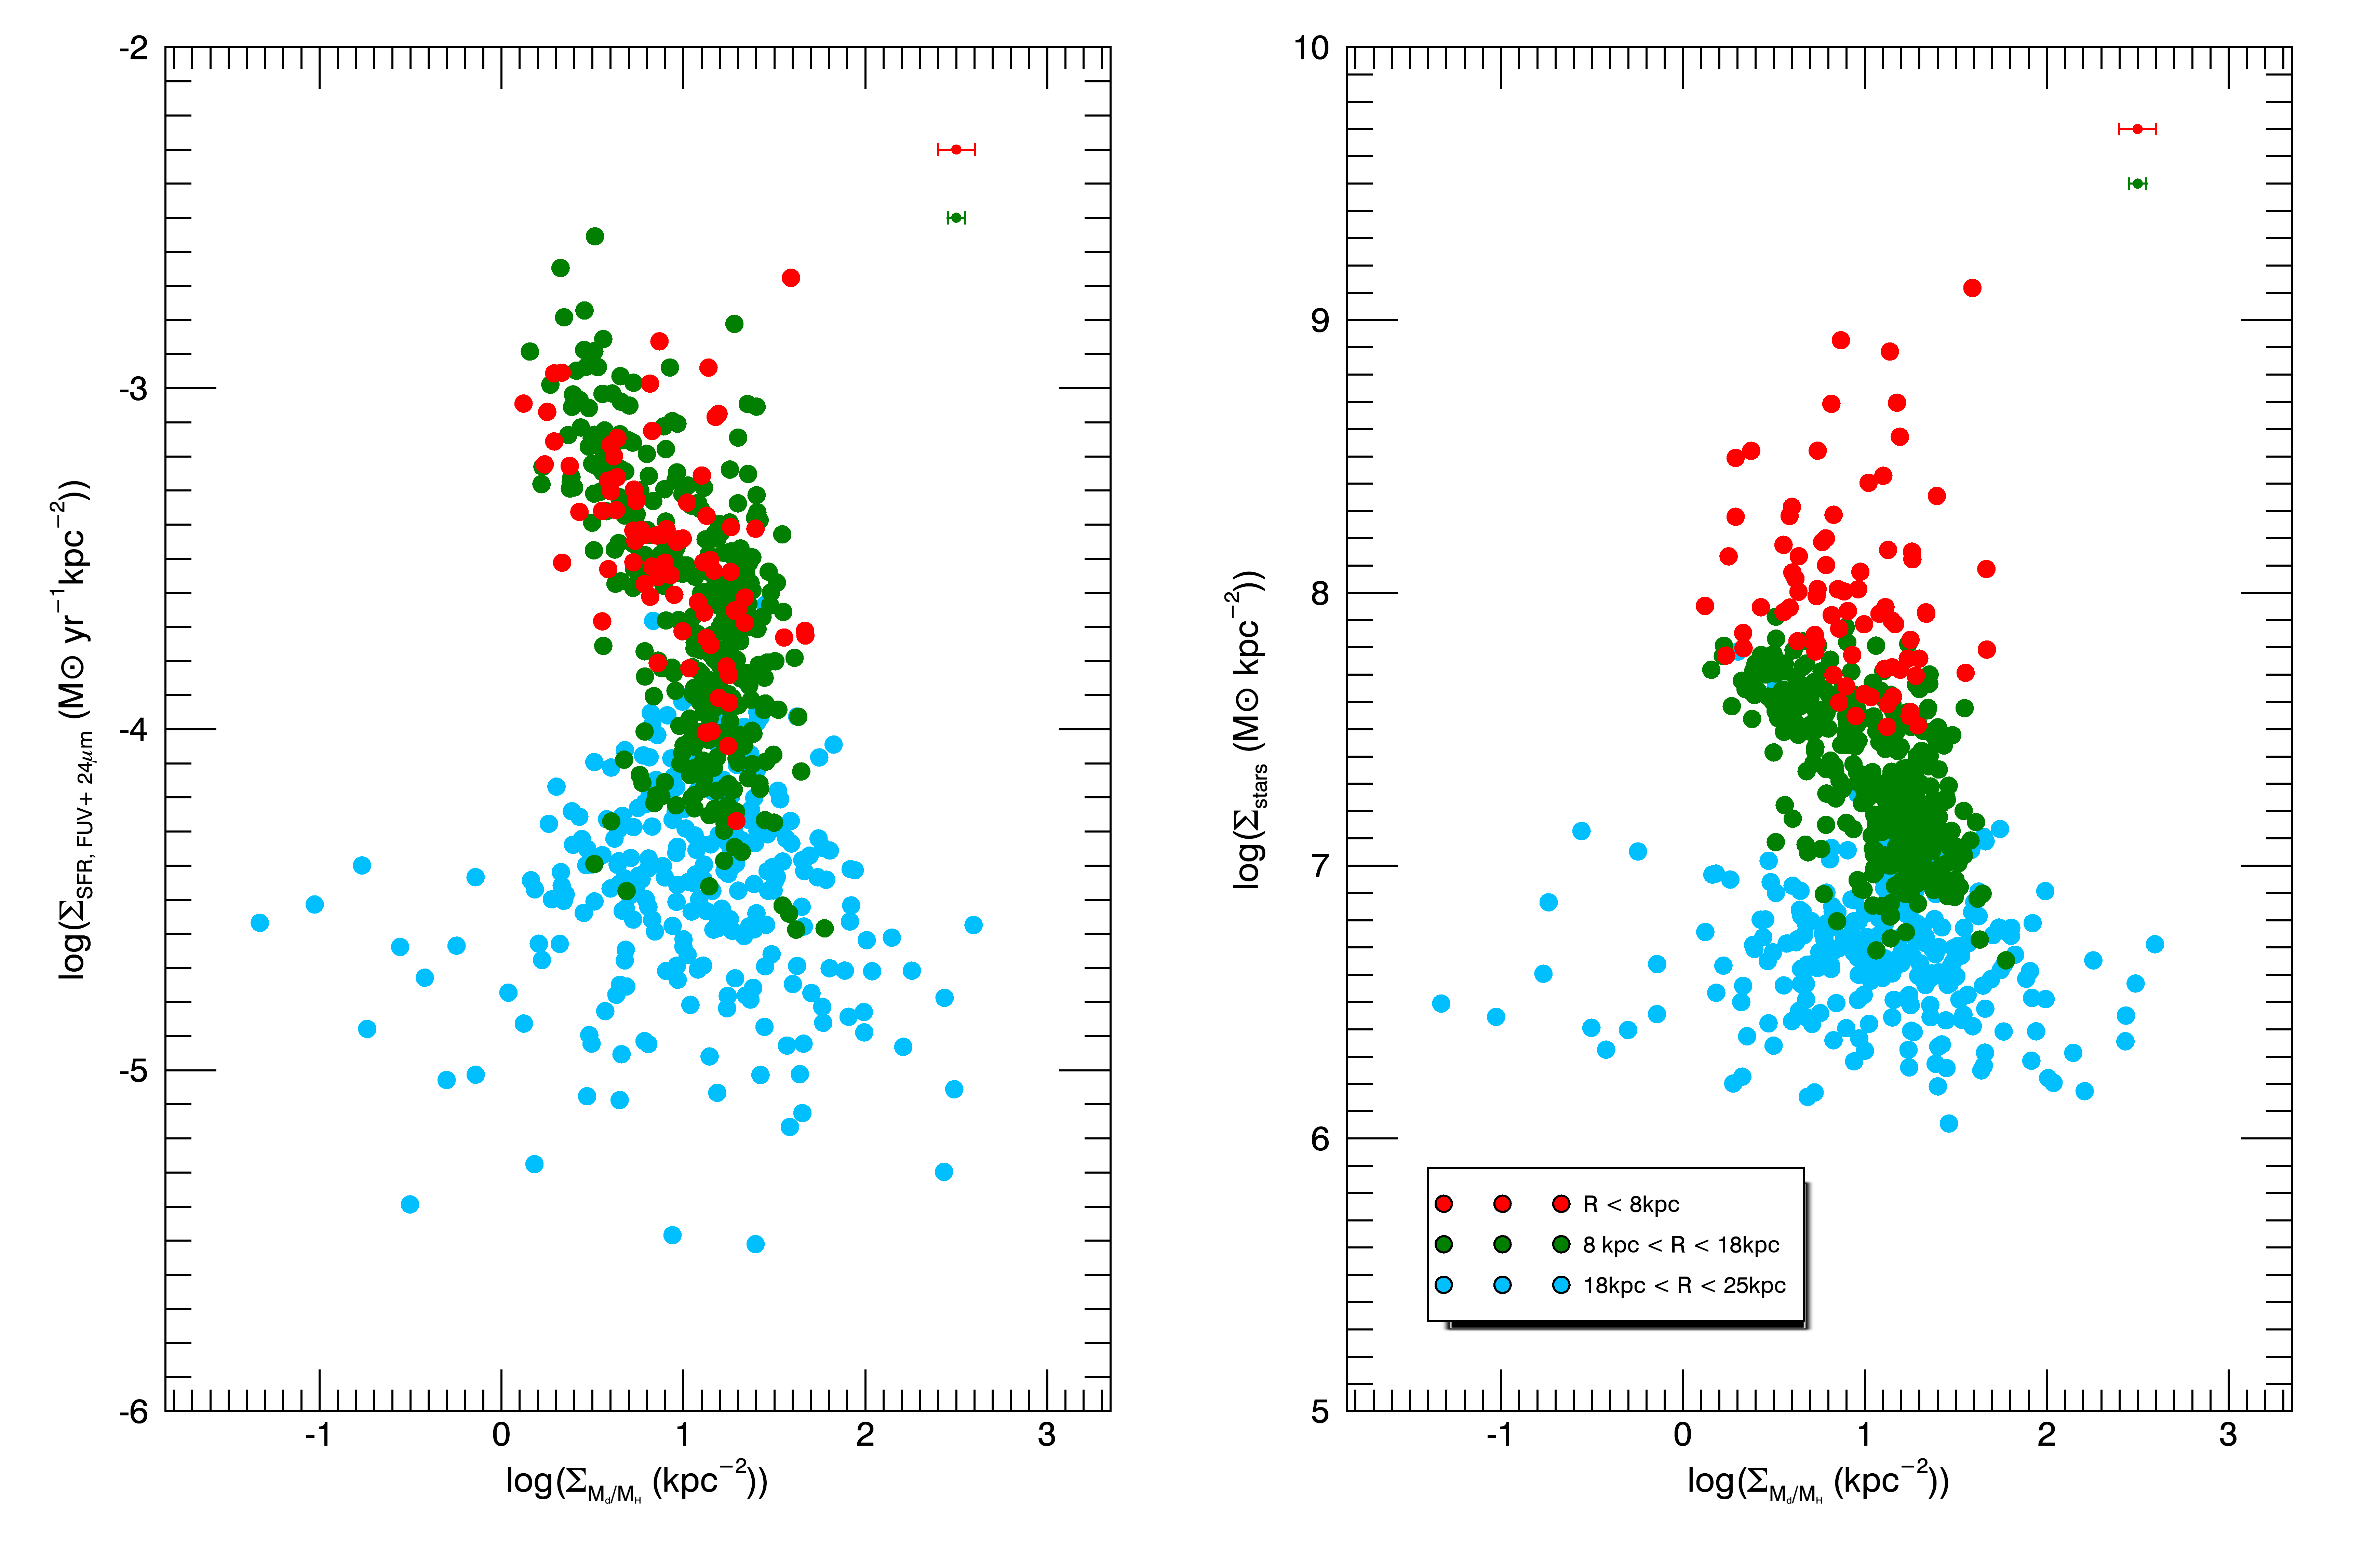
\includegraphics[width=180mm]{../image_paper1/metal_with_errors.png}
    \caption{Left: the SFR(FUV + 24~$\mu$m) surface density versus gas/dust mass ratio surface density and right: Stellar mass versus gas/dust mass ratio surface density  shows the stellar mass. Each point shows a region with size of $\sim$750~pc. Typical uncertainties of the x-axes within 18~kpc are shown in upper right side of the plots. The regions with $R< 8\kpc$, $8\kpc < R < 18\kpc$, and $18\kpc < R \la 25\kpc$ are shown in red, green and blue, respectively.}
    \label{fig:metal}
\end{figure*}

%----------------------------------------------------------------------------------------
%SUMMERY
%----------------------------------------------------------------------------------------
\section{Summary}
 We investigated the K-S law, the extended Schmidt law and the Krumholz law at both global and local scales in M31. We have determined the surface density of star formation rate, gas mass and stellar mass of this galaxy. Our three SFR maps in M31 use a combination of the FUV and 24~\um emission, a combination of the H$\alpha$ and 24~\um emission, and total infrared luminosity. We noticed that the H$_\alpha$ data available for M31 is not suitable for SFR studies (see appendix ~\ref{app:halpha}). We calculated the total SFR from FUV and 24 \um emission as 0.31$\pm$ 0.04 M$_{\odot}$yr$^{-1}$. We also produced the ISM map, using molecular gas only, atomic gas only and the total gas. Our main results are as follows:
\newline
1) The power-law index of the K-S law is mostly depended on which gas is used as a tracer of the gas mass in galaxy. Power-law indices are mostly independent of the SFR tracer.
\newline
2) Using different fitting methods gives different results. This dependence mostly comes from the way each fitting method handles the uncertainty on the star formation law parameters.
\newline
3) Although there is a correlation between \sigmasfr and \sigmagas, it is not the same in all regions in M31. The star formation laws predict more accurate results on regions with relatively higher star formation. 
\newline
4) We confirmed the suggestions of \citet{Shi11} that the surface density of stars has an impact on the SFR, and in regions with low gas surface brightness this impact is even more important. 
\newline
5) We performed statistical tests and found no correlation between the SFR, the stellar mass surface density and metallicity in the case of the whole galaxy. However there is a weak correlation between these quantities within 18~kpc of the centre of the galaxy.
\newline 
Obtaining images with higher resolution and maps with better coverage of this galaxy will enable continuation of these studies in finer detail.

\addcontentsline{toc}{section}{Bibliography}
\bibliographystyle{apj.bst}
\bibliography{ref_paper1.bib}
\chapter{Data Mining in Nearby Galaxies}
\label{ch: paper3}
%----------------------------------------------------------------------------------------
%----------------------------------------------------------------------------------------
%----------------------------------------------------------------------------------------
%Intro
%----------------------------------------------------------------------------------------
%----------------------------------------------------------------------------------------
%----------------------------------------------------------------------------------------
\section{Introduction} 
% Nearby galaxies and their importance 
Nearby galaxies play an important role in our understanding of galaxies' formation and evolution.
Nearby galaxies are defined as those close enough that we are able to observe their structure and composition in detail.
As a result, many studies have been devoted to finding relations between physical properties of galaxies, such as morphology, star formation rate (SFR), stellar mass, metallicity, and amount of gas, both for spatially-resolved regions and galaxies as a whole~\citep[e.g.][]{Wong13,Leroy08}, and many others use these results in analyzing observations of high-redshift galaxies~\citep[e.g.][]{Freundlich13,Walch11}.
Surveys such as KINGFISH~\citep{Kennicutt11} and THINGS~\citep{Walter08} have made observations of nearby galaxies in various wavelengths and from these data we can measure physical properties such as stellar mass, star formation rate (SFR), dust mass, and gas mass~\citep[e.g.][]{Eskew12,Dale09,Calzetti07}.

% A little bit about M31 and previous studies in M31.
The Andromeda galaxy (M31), at a distance of $\sim$~0.78~Mpc, is the closest spiral galaxy to the Milky Way~\citep{McConnachie05}.
Images of this galaxy provide us with a detailed view of the inside of a spiral galaxy as seen from an external perspective.
M31 has been observed by many telescopes including the {\textit {Hubble}}, \Spitzer and \Herschel space telescopes. %Els: Use the correct names for telescopes?
\cite{Barmby06} used data from the \Spitzer Infrared Array Camera \citep[IRAC;][]{Fazio04} to show the spatial distribution of Polycyclic Aromatic Hydrocarbons (PAHs) in the interstellar medium (ISM) of M31.
Using data from the Multiband Imaging Photometer for Spitzer (MIPS) instrument, \cite{Gordon06} studied the morphology of M31's dust.
\cite{Azimlu11} and \cite{Sanders12} catalogued and studied \hii~regions of M31.
\cite{Draine14, Mattsson14, Viaene14, Smith12} and~\cite{Fritz12} used \Herschel data to study dust in the ISM of the galaxy.
Properties of the current stars in the galaxy were studied by many groups~\citep[e.g.][and references therein]{Tamm12,Dalcanton12,Massey07}.
\cite{Rahmani16, Ford13} and \cite{Tabatabaei10} measured the spatially-resolved SFR in M31 in order to study star formation laws, and~\cite{Dim15} and \cite{Kapala15} used infrared spectroscopy to study PAHs and atomic and molecular line emission in the ISM.

Although all these studies measured some properties of M31, or answered specific scientific questions about this galaxy, we still do not have a complete picture of underlying processes in the galaxy.
What is the correlation between PAHs and SFR, dust mass, and gas mass in M31? 
Are PAH features in M31 similar or they can be divided into various groups? If so, what are the properties of each group?
Does the intensity of PAH emission depend on location or global galaxy properties? 
The properties of M31 that derived in various studies and observational data of this galaxy can be used for a knowledge discovery and data mining study.
The Pinwheel Galaxy (M101), with distance of 6.7~Mpc~\citep{Freedman01}, is another nearby galaxy that has been well-observed and studied~\citep[e.g. ][and references therein]{Kennicutt11,Dale09, Leroy08, Gordon08}.
M101 is a large spiral galaxy with several \hii~regions and a large metallicity gradient from centre to outskirts~\citep{Kennicutt03}.
Since the observational data from M31 and M101 are similar, M101 is a suitable addition to M31 data for a data mining study. 
Knowledge discovery and data mining methods are designed to extract hidden information from data and have been tested in many astronomical studies~\citep[e.g.][and references therein]{Ball10}.
However, this study is the first to use a data mining method on observations of nearby galaxies.

% data mining and clustering in general; when we have so many data and we want to map them
\cite{Ball10} gave an extensive review of data mining and machine learning algorithms and their usage in astronomy.
A data mining algorithm learns about data from training, which can be supervised or unsupervised.
Supervised training refers to methods that use examples of the desired output to learn about input data; these are valuable tools for classifying data with known target values.
Unsupervised methods train without any prior knowledge of output results: 
they work solely based on the underlying structure of the input data.   
The unsupervised methods are very useful tools in knowledge discovery studies, where we have limited pre-expectations for the data or when we want to make sure that we did not miss any valuable information in previous studies.

The purpose of the present work is to use M31 observations to provide new insights into nearby galaxies, with a focus on relations between PAHs and other properties of the galaxy,
as there are few studies on relations between properties of M31 with its PAH features.
\cite{Cesarsky98} studied PAH spectra observed by ISOCAM spectro-imaging in four regions in M31 and found that PAH features in M31 differ from those in other galaxies in having weak or no $6.2 - 8.6$~$\mu$m emission with enhanced 11.2~$\mu$m emission. 
However,~\cite{Dim15} using {\it Spitzer}/Infrared Spectrograph~\citep[IRS;][]{Houck04b} observations, found that the PAH spectra of M31 have the same features as the spectra of other nearby star-forming galaxies.
Those authors re-evaluated the ISOCAM data to compare them to IRS data and found that the earlier results were likely due to incorrect background subtraction.
Using IRAC imaging observations,~\cite{Barmby06} found good agreement between the M31 SFR derived using observed 8~$\mu$m luminosity with other 
star formation indicators such as \halpha and far infrared luminosity.
\cite{Draine14} found that the PAH abundance in M31 is almost constant up to a galactocentric radius of $\sim 20$~kpc.
With data mining techniques we address the question of whether,
compared to other galaxies, PAH features in M31 are unique as~\cite{Cesarsky98} claimed, or  are normal as ~\cite{Dim15} and \cite{Draine14} concluded.


%this project 1 M31 and its extensive data we do not have any SOM in nearby galaxies
In this project we apply the self-organizing map algorithm (SOM) to M31 data, training 1D and 2D networks.
Using networks with fewer neurons, we study the properties of the clusters and investigate relations between PAH features and other quantities in M31.
We create 2D SOMs from subsets of the data as well as all available data, which helps us to understand the effect on each input on the position of the clusters in the SOM.
We apply the 2D trained networks to the M101 data to study whether they have similar properties to M31 ones.
If our hypothesis is correct, we should be able to see that regions in M31 and M101 with the same positions in the SOM have the same properties.


We describe the SOM method in $\S$~\ref{sec: method_SOMN}. 
In $\S$~\ref{Sec: data_SOMN}, we present the observational data from M31 and M101 that we use in this study.
The results of the 1D SOM networks and the study of PAHs in M31 are presented in $\S$~\ref{Sec: 1d_cluster}.
In $\S$~\ref{sec: 2d_cluster}, we present the results of 2D SOM networks and their use in extracting information about other galaxies.
In $\S$~\ref{sec: summary}, we summarize our results and discuss potential future work in this subject.
%----------------------------------------------------------------------------------------
%----------------------------------------------------------------------------------------
%----------------------------------------------------------------------------------------
%Method
%----------------------------------------------------------------------------------------
%----------------------------------------------------------------------------------------
%----------------------------------------------------------------------------------------
\section{Method}
\label{sec: method_SOMN}
\subsection{Choosing an Algorithm}

Some of the most tested methods of data mining in astronomy are artificial neural networks (ANNs)~\citep[e.g.][and references therein]{Hossein14,Hossein16}.
ANNs are spiered to work in the same way that the neurons work in a human brain.
These are networks of interconnected neurons (nodes), in which all of the connections are weighted.
These networks are used to study nonlinear and complex relations between input and output data.
One of the most well-known unsupervised neural networks in astronomy is a Kohonen self-organizing map (also called self-organizing map, or SOM).
SOMs visualize complex data~\citep{Kohonen82} and show simple geometrical relationships in non-linear high dimensional data~\citep{Kohonen98}.
The result of a SOM is a 1D or 2D network of neurons, which shows the positions of clusters and their relative distance.
Since the 1990s, many studies have utilized SOMs for object classification and clustering (e.g. classifying quasars' spectra, star/galaxy classifications, gamma-ray burst clustering and light curve classification) and photometric redshift estimation~\citep[e.g.][]{Odewahn92, Hernandez94, Murtagh95, Maehoenen95,Scaringi09,Geach12,Fustes13,Meusinger16}.

The K-means algorithm, SOMs, and hierarchical clustering are the main unsupervised methods that are used in astronomical studies~\citep[e.g.][]{DAbrusco12, Aycha16}.
For K-means algorithms, the user must define the number of clusters and for and SOM algorithms the user defines the number of neurons, and the algorithms decide how to separate the data into clusters.
In the hierarchical clustering method, the user must define dissimilarity between the groups; the algorithm combines (or divides) existing groups based on their dissimilarity and creates a hierarchical structure. 
Comparing the SOMs, K-means and hierarchical clustering methods shows that in some cases the hierarchical clustering method mis-classifies the data~\citep[][and references therein]{Mangiameli96}.
We chose the SOM method over the K-means method due to the fact that SOMs not only cluster data, but also show similarities and dissimilarities between the clusters.
Therefore, we can cluster our sample data and study the underlying structure simultaneously.

     
    \subsubsection{Algorithm of SOM} 
   \label{sec: algorithm_somz}
    The self-organizing map is a clustering method which reduces the dimension of the data, usually to one or two dimensions (1D or 2D), while preserving topological features of the original dataset.
    The result of an SOM is a set of nodes (neurons) that are arranged in a 1D or 2D arrays \citep{Kohonen98}. 
    Each node may contain one or more samples from the input data.
    The distance between the nodes represents similarity or dissimilarity of the underlying samples, i.e., similar data are closer together in the array and the distance between two nodes is related to the dissimilarity of their samples.
    A weight vector ``\boldit{W}" with the same dimension as the input data is associated with each node and will be varied during the training process.
    This vector is the key factor in determining the position of the nodes in a map.
    \cite{Geach12} presented the application of the SOM and discussed its algorithm in detail.
    In this section we briefly discuss the algorithm of SOM, how we create our maps and a present a  test model which will help interpretation of our results. 
   
     Assume we have a dataset which contains vectors, \boldit{V} $\in \Re^n$, and we want to map them on an S1 by S2 map. 
     We start by creating S1 $\times$ S2 empty neurons. 
     The initial arrangement of these neurons depends on the map's topology provided by the user.
     In the case of 1D maps, since each neuron has two immediate neighbours, the topology of the map does not have any effect on the final result and any topology can be chosen.
     However, in 2D maps, the shape of the neurons specifies the number of immediate neighbours for each neuron and it is up to user to choose the most suitable shape based on the data.
     In this chapter, we choose hexagonal topology, which gives each neuron six neighbours, and provides more interactions between neurons.
     Initially a random weight vector, \boldit{W} $\in \Re^n$, will be assigned to each node.
     The process of creating SOM happens over a series of $N$ iterations. 
     During each iteration the weight vectors might change according to the Kohonen learning rule (equation~\ref{equ: weight adj_SOMZ}). 
      In each iteration, the SOM code:
     \begin{enumerate}
        \item chooses a random vector from the dataset ($V_i$).
        \item calculates the Euclidean distance for each node, $j$, as  $D_j^2= \sum_{i=0}^{i=n} (V_i - W_i)^2$, and finds a neuron with minimum $D_j$, (``$D_{j_{min}}$"). This neuron is the winner node and is called the Best Matching Unit (BMU). 
        \item  computes the radius of the neighbourhood of the BMU to find nodes within this radius. The weight vectors of these nodes will be affected in the next steps. The radius of the neighbourhood is arbitrary and can be set to be as high as half of the SOM size. It then decays exponentially over each iteration as
        \begin{equation}
            r^t_{BMU} = r^0_{BMU}e^{(-t/\tau)}
        \end{equation}
        where $\tau$ is a decay constant and is usually set to be the same as the number of iterations, $N$. $r^0_{BMU}$ and $r^t_{BMU}$ are the radii of the neighbourhood at 0th and $t$th iteration, respectively. 
        \item changes the weight vectors of the BMU and all the nodes within $r^t_{BMU}$ as:
        \begin{equation}
            \label{equ: weight adj_SOMZ}
            w(t+1)=w(t)+L(t) \times R(t) \times(v(t)-w(t))
        \end{equation}
        where $L(t) = L_0 e^{(-t/\tau)}$ is the learning factor, which prevents the divergence of the SOM and $R(t)=\exp(-\frac{D_j^2}{2r^t_{BMU}})$ is the influence rate. $R(t)$ determines how the weight of each node in the neighbourhood of BMU will change.
     \end{enumerate}
     These steps are then repeated $N$ times.
     
\subsection{Creating Self-Organizing Maps}
\label{sec: create_som}
     In order to create SOMs, we use the {\sc matlab} neural network toolbox~\citep[NNT,][]{matlabtolbox}.
     
     SOM in {\sc nnt} can be created by using the {\sc newsom} or {\sc selforgmap} libraries, both of which work in two phases, an ``ordering phase" and a ``tuning phase". 
     The first phase is called the ``ordering phase" and
     starts with maximum neighbourhood distance and an initial high learning factor (usually 0.9) is provided by the user. 
     The ordering phase continues for a requested number of iterations.
     During the iterations, the learning factor decreases to the tuning phase learning factor and the neighbourhood distance reaches that of the tuning phase as well.
     Both the learning factor and the neighbourhood of the tuning phase are set by the user. 
     The amount by which these two factors change in each iteration depends on the number of iterations.
     
     In the second, or ``tuning'' phase,
     the neighbourhood distance is kept at the user-defined minimum.
     The learning factor, however, decreases gradually.
     The gradual change in the leaning factor helps to fine-tune the topology results, leading to a more stable SOM. 
     To allow the fine tuning, the number of iterations in this phase must be much larger than the that of the ordering phase.
     We chose the number of epochs in the tuning phase to be 3 times the number of epochs in the ordering phase.
     
     To present our results, we use \textsc{nnt}'s built-in plotting tool.
     Specifically, we combine two of the plots in this tool: a hits map, which shows the number of times each neuron has become the winner (hits), and a distance map, which shows the distance between weight vectors of those neurons.
     In the maps, the purple hexagonal shapes show the neurons. 
     The distances are shown by the grey-scale colours: the darker the colour, the larger the distance between neurons.
     Neurons with zero hits are left empty.
     In Section~\ref{sec: mock_sample} we used \textsc{newsom} to create SOMs from a mock sample to illustrate how this method works and how to interpret the results.
      
    The sizes of the SOM maps are arbitrary and there are no rules regarding choosing one over the other. 
    \citet{Vesanto05} suggested that a total number of $5\sqrt{n}$ neurons is a sufficient size, but users usually choose the size of the grids based on their dataset and their application of the results.

\subsection{Mock Sample}
\label{sec: mock_sample}
 
         \begin{figure}
                \centering
                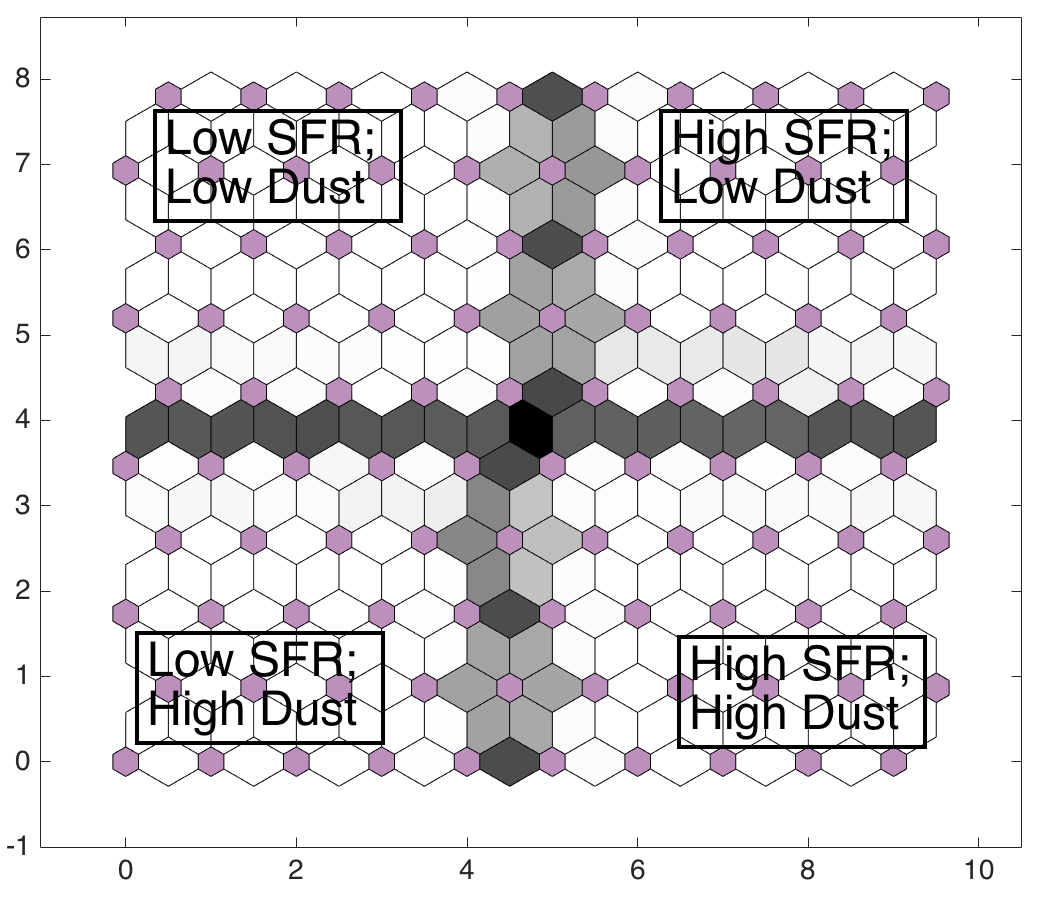
\includegraphics[width=\textwidth]{../image_paper3/images0.01/mock_sample.png}
            \caption[Self-organizing map of the mock sample]{SOM of the mock sample. The axes show the position of the neurons. Hexagonal shapes represent the neurons. The grey-scale colours show the differences between neuron weights, where white is the minimum difference and black is the maximum one.}
            \label{fig: sample}
        \end{figure}
 
To show how self-organizing maps work, we created a mock sample containing only a few regions.
Each sample had two properties: the amount of dust and the star formation rate, where the possible values were
either 0 or 1 for low or high SFR, and 0 or 0.5 for a low or high amount of dust. 
 We generated an SOM from the sample with a size of $10 \times 10$, using the method described in Section~\ref{sec: method_SOMN}.
 Fig.~\ref{fig: sample} shows the SOM of the mock sample. 
 The axes show the position of the neurons in a $10 \times 10$ network and the hexagonal shapes (depicted by purple hexagons) are the neurons.
 
Using this method, as expected, we are able to divide the mock sample into 4 distinct groups. Their boundaries are shown by grey colours in Fig.~\ref{fig: sample}: regions with high SFR and high dust content, regions with low SFR and high dust content, regions with high SFR and low dust content, and regions with low SFR and dust content. 
In Fig.~\refthere ha{fig: sample}, the upper part belongs to regions with low dust content, while the lower part belongs to regions with high dust content.
The left part of the plot is where regions with low SFR belong and the right side is for high SFR regions.
Grey to black colours show the border between regions.
This network is considered to be a trained network, and can be used to cluster any new data set with similar entries.

Having two regions with exactly the same values in all their quantities with real data is extremely unlikely. 
If, in an input data set, there are two entries with similar (but not identical) values in all dimensions, one can find a network that separates these two entries in two groups.  
However, in case of multiple similar entries in a dataset, the number of neurons must be much higher than the number of entries for complete separation.
Therefore, the user learns about similarity or dissimilarity of members of the input dataset based on the ratio of the number of entries in the dataset and  the number of neurons. 

%----------------------------------------------------------------------------------------
%----------------------------------------------------------------------------------------
%----------------------------------------------------------------------------------------
%DATA
%----------------------------------------------------------------------------------------
%----------------------------------------------------------------------------------------
%----------------------------------------------------------------------------------------
\section{Study Sample}
\label{Sec: data_SOMN}

Our study includes 10 regions in M31 (Fig.~\ref{fig: regions in m31}) and 8 regions in M101 (Fig.~\ref{fig: regions in m101}). 
These specific regions were chosen for the availability of \Spitzer/IRS 5--15$\mu$m  spectroscopy covering the PAH emission bands.
Besides PAH band strengths, for each galaxy, we use spectroscopic and photometric observations as well as their derived properties, such as SFR, stellar mass, dust luminosity (L$_{\rm dust}$), dust mass, metallicity, and gas mass.
Table~\ref{tab: data} shows the full list of data for both M31 and M101.
All data were divided by the area of their region (in arcsec$^2$), to remove the distance factor from the data and compare values across galaxies.
Since the spatial resolution of the observations varies from as small as $<1$\arcsec to as high as 60\arcsec $\times$ 90 \arcsec, any attempt to match resolution would have caused a loss of information in some of the input quantities (e.g. the spectroscopic data).
In this project we used flux per unit area, which the convolution methods conserve~\citep{Aniano12}, as the input data.
Therefore, we did not perform any resolution matching and used data at their original resolution.

    \import{../image_paper3/text_files/tables/}{tab_data.tex}

    \begin{figure}
  \begin{subfigure}[b]{\textwidth}
        \centering
        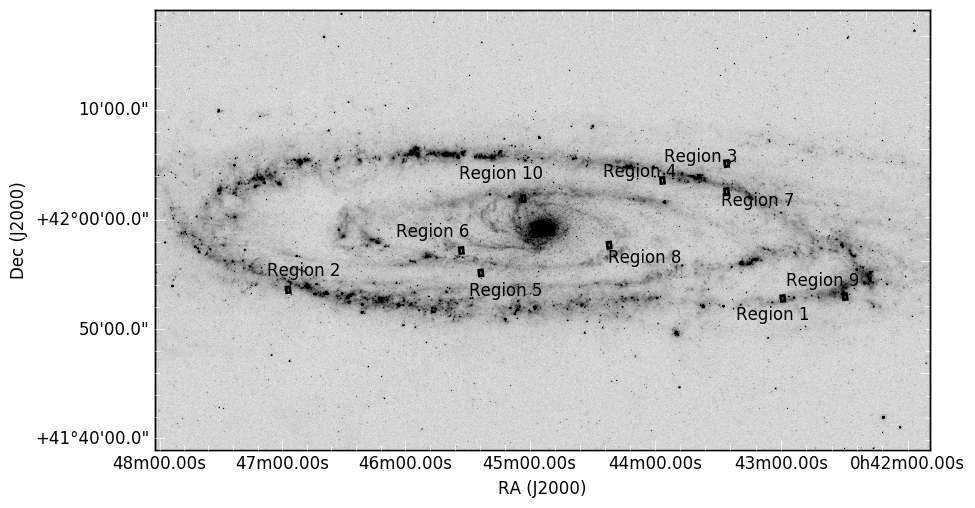
\includegraphics[width=0.97\textwidth]{../image_paper3/images0.01/M31/M31.png}
        \caption{MIPS~24 $\mu$m image of M31, with positions of 10 regions studied.}
        \label{fig: regions in m31}
    \end{subfigure}
    \hfill
    \begin{subfigure}[b]{\textwidth}
        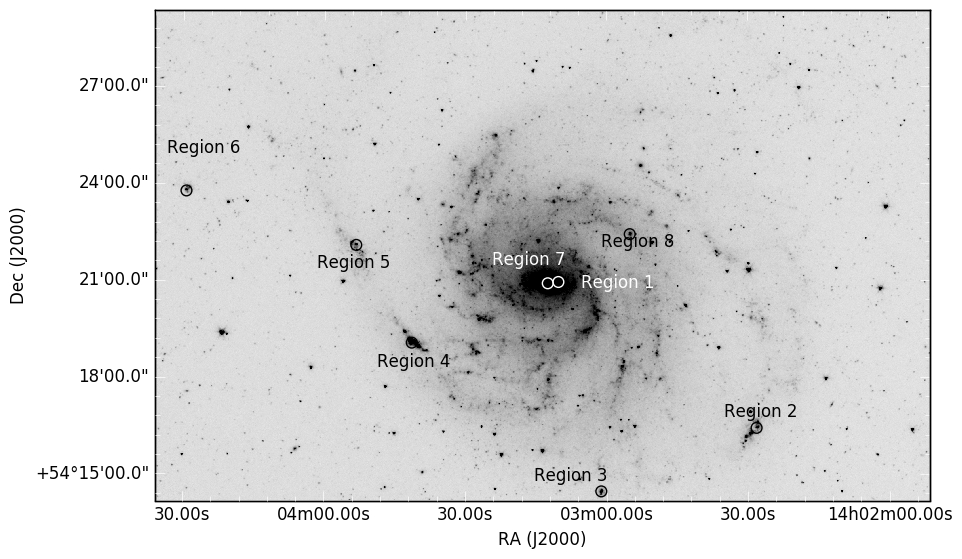
\includegraphics[width=\textwidth]{../image_paper3/images0.01/M101/M101.png}
        \caption{IRAC 3.6 $\mu$m image of M101, with positions of  8 regions studied.}
    \label{fig: regions in m101}
    \end{subfigure}
    \caption[Position of the data in M31 and M101]{Position of the data in M31 (a) and M101 (b).}
\end{figure}

    \subsection{M31 Observations}
     \label{Sec: data_M31_SOMN} 
     
     \cite{Dim15} used {\it Spitzer}/IRS observations to study PAHs in 10 regions chosen to span a range of mid-infrared flux ratios in M31 (Fig.~\ref{fig: regions in m31}). 
     Fluxes and equivalent widths of PAH and atomic line features were measured using the~\textsc{pahfit idl} tool~\citep{Smith07b}.
     Metallicity for all regions except regions 5 and 8 were adapted from~\citep{Sanders12} and for regions 5 and 8, \cite{Dim15} estimated metallicity from the radial metallicity profile.
     \cite{Dim15} also measured radiation hardness index (RHI) using calibration of the ratio of two lines, $\left (\log \frac{[Ne~\textsc{iii}]}{[Ne~\textsc{ii}]} + \left [ 0.71 + 1.58\log\frac{[S~\textsc{iV}]}{[S~\textsc{iii}]} \right ] \right )/2$, for these 10 regions.
     We used the measured PAH feature fluxes, metallicity and RHI of each region as the input for self-organizing maps.
     
    For the photometry part of the sample, we used the \GALEX \citep{Martin05} far-ultraviolet and near-ultraviolet (FUV and NUV) channel images; \halpha~(6574.7\AA), \sii~(6730.72\AA) and \oiii~(5024.9\AA) narrow band images~\citep{Massey07}, IRAC 3.6, 4.5, 5.8 and 8.0~$\mu$m images~\citep{Barmby06}; MIPS~24 and 70~$\mu$m~images~\citep{Gordon06}; and PACS 100 and 160~$\mu$m and SPIRE 250, 350, and 500~$\mu$m~\citep{Fritz12} images.
     The units of all fluxes were converted to W~m$^{-2}$ in order to be the same as the PAH fluxes.
     $^{12}$CO (J:$1\rightarrow0$) line emission images~\citep{Nieten06} and atomic gas (\hi) 21~cm emission images from~\cite{Chemin09} were added to the input data. 
     For derived values, we utilized SFR(FUV + 24$\mu$m) measured using combination of FUV and 24$\mu$m emission, stellar mass, molecular gas mass, atomic gas mass, total gas mass, and total infrared (TIR) luminosity (L$_\mathrm{TIR}$) from~\cite{Rahmani16}, and L$_\mathrm{dust}$ and dust mass from~\cite{Draine14}.
     
    \subsection{M101 Observations}
    \label{Sec: data_M101_SOMN} 
    
     \cite{Gordon08} measured PAH fluxes and RHI for M101 in 8 star forming \hii~regions (Fig.~\ref{fig: regions in m101}).
     Metallicities of 6 of the 8 regions were measured by~\cite{Kennicutt03} and the other two by~\cite{Gordon08}.
     We used the NED~\footnote{The NASA/IPAC Extragalactic Database (NED) is operated by the Jet Propulsion Laboratory, California Institute of Technology, under contract with the National Aeronautics and Space Administration.} website to gather imaging observations of M101, including 
      \GALEX FUV and NUV~\citep{depaz07}, IRAC 3.6 -- 8.0~$\mu$m, MIPS~24 and 70~$\mu$m~\citep{Dale09}, and PACS~100 and 160~$\mu$m and SPIRE~250, 350, and 500~$\mu$m emission from~\cite{Kennicutt11}.
     As with M31, we used $^{12}$CO (J:$1\rightarrow0$) line emission images~\citep{Helfer03} and atomic gas (\hi) 21~cm emission images from \cite{Walter08}.
     We calculated SFR(FUV + 24$\mu$m), stellar and total gas mass maps using the same methods as for M31.
     
     \subsection{Preparing Data for Data Mining}
    
     Correlations between some of single-wavelength emission and galaxy properties are well-known.
     Emission in the 3.6$\mu$m band traces the old stellar population very well~\citep[e.g.][]{Smith07a,Leitherer99} and it can be used to calculate the stellar mass~\citep{Eskew12}.
     FUV, \halpha, and TIR emission are indicators of star forming regions.
     In this project, we used the SFR traced by the FUV emission, corrected for foreground stars using NUV emission and for dust extinction using 24~$\mu$m emission.
     Total infrared emission is calculated from a modified version of~\cite{Draine07} calibrations using using 8, 24, 70, and 160~$\mu$m emission~\citep{Boquien10}.
    
    
    We removed all the observed data that were used to calculate galaxy properties from the input sample, to guarantee that they have not been used in multiple forms.
    To have prior knowledge of the M31 data set, 
    we computed the Pearson correlation coefficients between input measurements.
    Fig.~\ref{fig: cor_all} shows the Pearson correlation coefficients with a confidence level of 95 per cent. 
    If the significant level of correlation becomes smaller than 0.05 (5 per cent), the correlation is marked as insignificant. 
    All the PAHs correlate with one another very well.
    They are also highly correlated with the SPIRE and PACS emission, L$_\mathrm{dust}$, L$_\mathrm{TIR}$, SFR and metallicity.
    The fluxes from PAHs 7.7, 8.3, 12.7 and 17~$\mu$m show a weak anti-correlation with RHI.
    In general, PAHs in our data set are highly correlated with most of the other quantities. 
    
      \begin{figure}
        \centering
        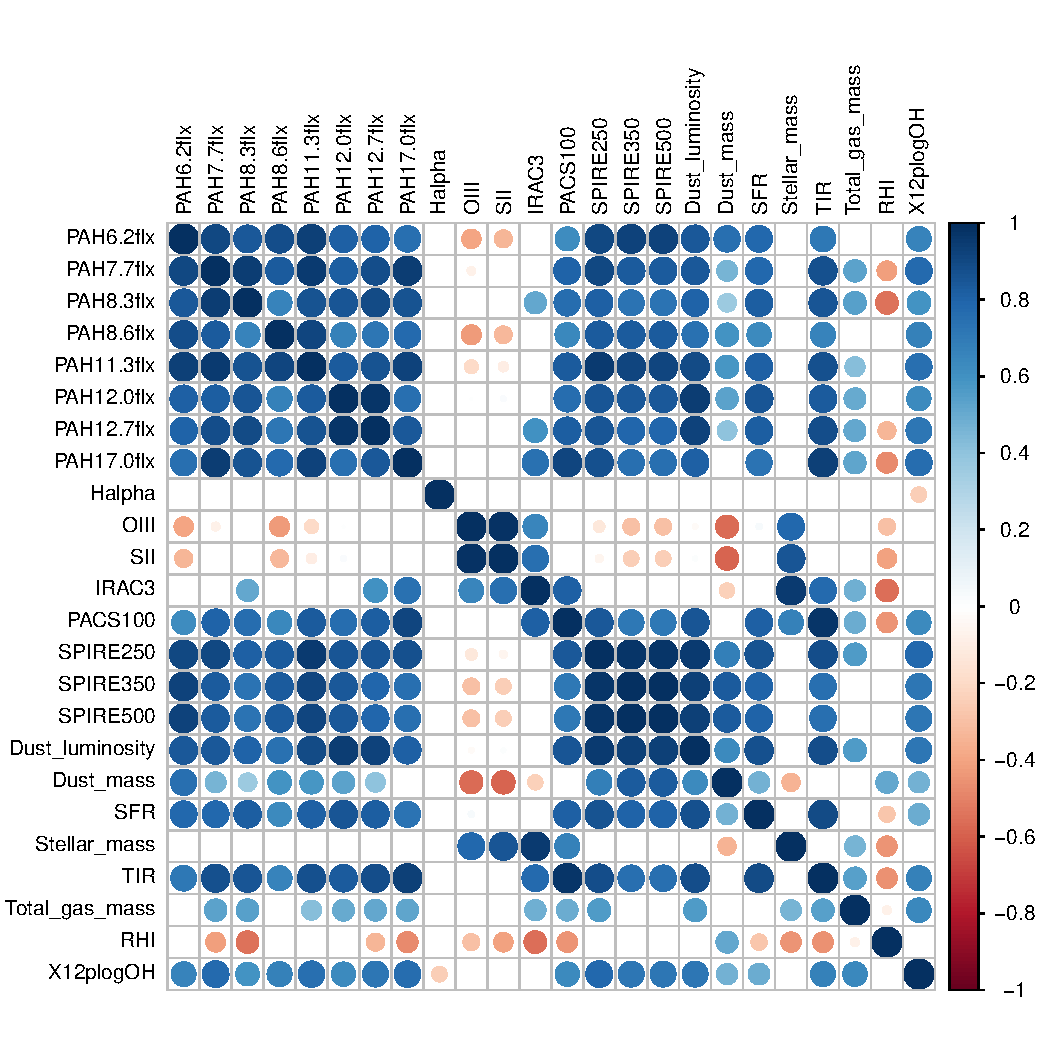
\includegraphics[width=\textwidth]{../image_paper3/images0.01/cor_plots/M31_all_derived_ones_core_plot_for_paper.pdf}
        \caption[Pearson correlation coefficients for data from 10 regions in M31]{Pearson correlation coefficients with a confidence level of 95 per cent for all data from M31. The colours and circle sizes show the Pearson correlation coefficients where large blue circles are 1, which means highly correlated, and large red circles are $-1$, which means highly anti-correlated quantities. The boxes with non-significant correlations were left empty.}
        \label{fig: cor_all}
    \end{figure}
 
 %----------------------------------------------------------------------------------------
%----------------------------------------------------------------------------------------
%----------------------------------------------------------------------------------------
%Result Part 1: 1D SOMs
%----------------------------------------------------------------------------------------
%----------------------------------------------------------------------------------------
%----------------------------------------------------------------------------------------
\section{One-Dimensional Self-Organizing Maps}
    \label{Sec: 1d_cluster}
%Why 1D maps are useful
    The purpose of  exploring the M31 data with 1D maps is to monitor the general behaviour of the data. 
    One-dimensional SOMs can have the minimum number of clusters, $1\times2$, up to the highest number of clusters possible (infinity). %Els asked what is maximum possible #
    In a small sample like ours, smaller grid SOMs are very useful to find correlations that cannot be found without  clustering the data.
    On the other hand, larger grid 1D SOMs are a helpful tool to get quick insight into the data.

    \subsection{Clustering M31 Data}

        In order to monitor how the data behave, we created SOMs with two to fourteen neurons (Fig.~\ref{fig: M31_nets_1d}).
        The $1\times2$ network (Fig.~\ref{fig: M31_net_1by2}) shows how the M31 data can be divided into two broad categories.
        The $1\times14$ network (Fig.~\ref{fig: M31_net_1by14}) is the first network in which all the regions in M31 are completely separated.
        In the higher network sizes, regions have more space to be separated based on their differences. In going from the $1\times2$ to the $1\times14$ network the distance between M31 regions increases, until they are completely separated. 
        
        Fig.~\ref{fig: M31_net_1by2} shows that by forcing the regions in the M31 to be divided into two groups, regions 1, 2, 9 and 10 (shown in Fig.~\ref{fig: regions in m31}) occupy one neuron and the other regions occupy the other one.
        The medium grey colour between two neurons indicates that there are some similarities between two groups, but they are not very similar. 
        By increasing the size of the neurons to three, in Fig.~\ref{fig: M31_net_1by3}, we can see that region 2 separates itself from the other regions and occupies the middle neuron.
        The white colour between the two left neurons suggests that the regions which occupy these neurons are very similar to each other, while the black colour between the two right neurons indicates otherwise.
        
        %%%Talking about four right regions
        \cite{Dim15} showed that regions 1, 2, 9, and 10 have higher PAH fluxes compared to the other regions (fig.~5 in \citealt{Dim15}). 
        These regions also have relatively high intensities in all the mid-infrared and far-infrared bands and have high dust luminosity and dust mass.
        The higher values for these quantities could be the reason that these four regions become separated from the others in the $1\times2$ network.
        Regions 1 and 9 are in the 10~kpc ring, region 2 is slightly out of the 10~kpc ring and region 10 is in the bulge of M31; however, regions 3 to 8 are located out of the inner ring or the 10~kpc ring (Fig.~\ref{fig: regions in m31}).   
        The differences in their positions account for their difference in input parameters.
        Since region 10 is located in the bulge of M31 and has high surface brightness for most of the input values, regions 1, 2, and 9 to gradually move towards other regions and away from region 10 in the higher grid SOMs.
       
    \begin{figure}
    \begin{subfigure}[b]{\textwidth}
        \centering
        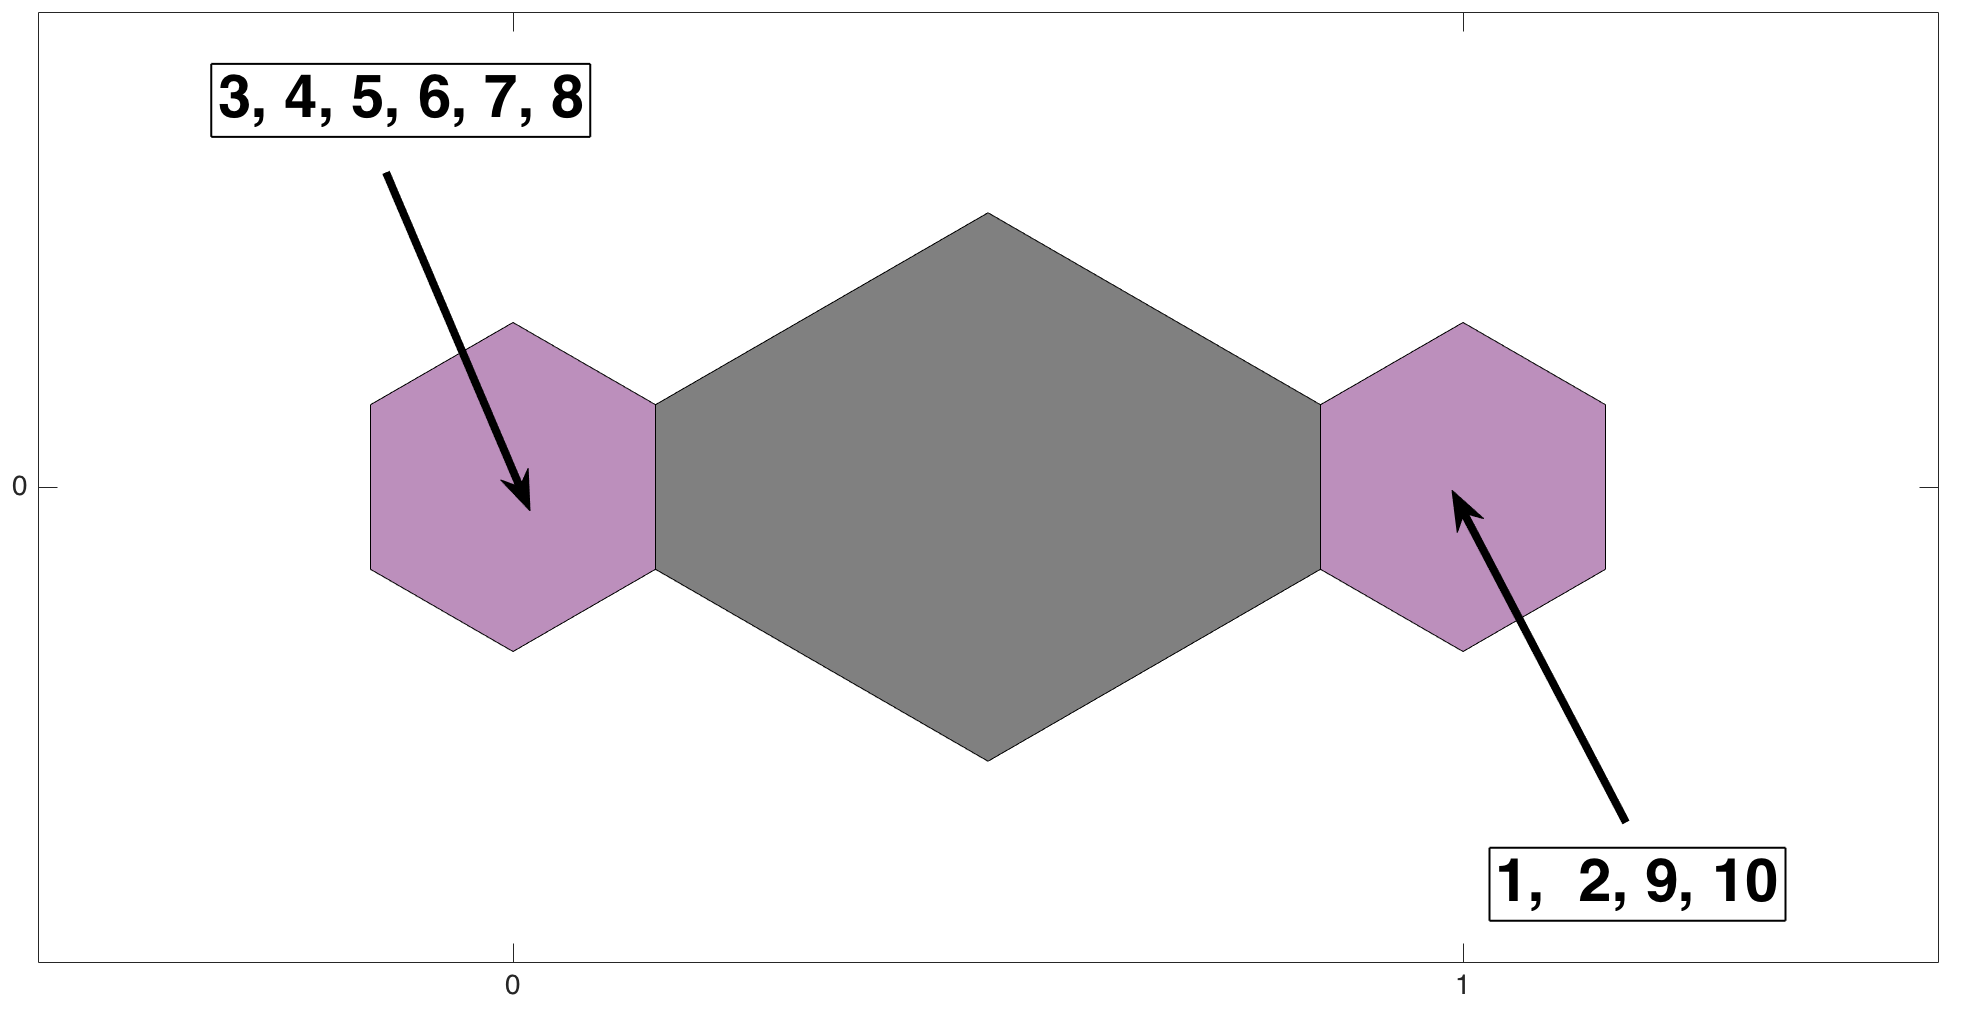
\includegraphics[width=\textwidth]{../image_paper3/images0.01/M31/1D/combine_1D_1by2_all.png}
        \caption{$1\times2$~network}
    \label{fig: M31_net_1by2}
    \end{subfigure}
    \hfill
    \begin{subfigure}[b]{\textwidth}
        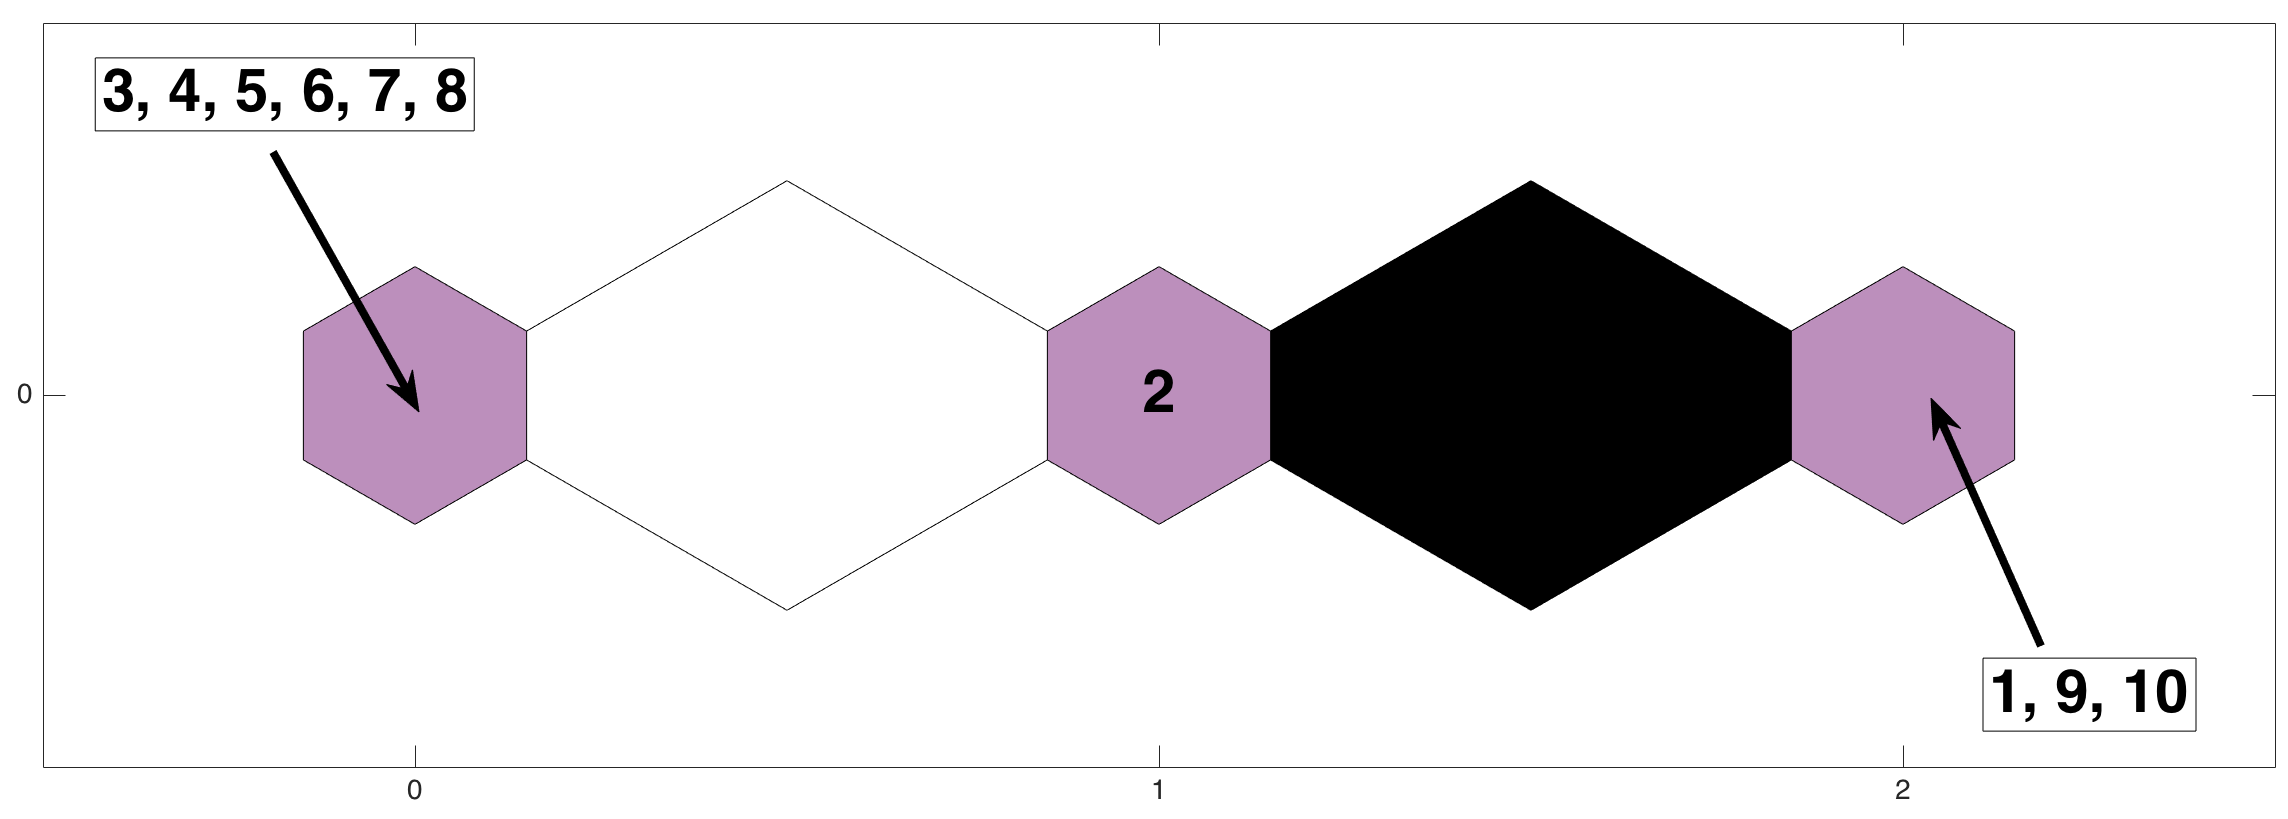
\includegraphics[width=\textwidth]{../image_paper3/images0.01/M31/1D/combine_1D_1by3_all.png}
         \caption{$1\times3$~network}
        \label{fig: M31_net_1by3}
    \end{subfigure}
    \hfill
    \begin{subfigure}[b]{\textwidth}
        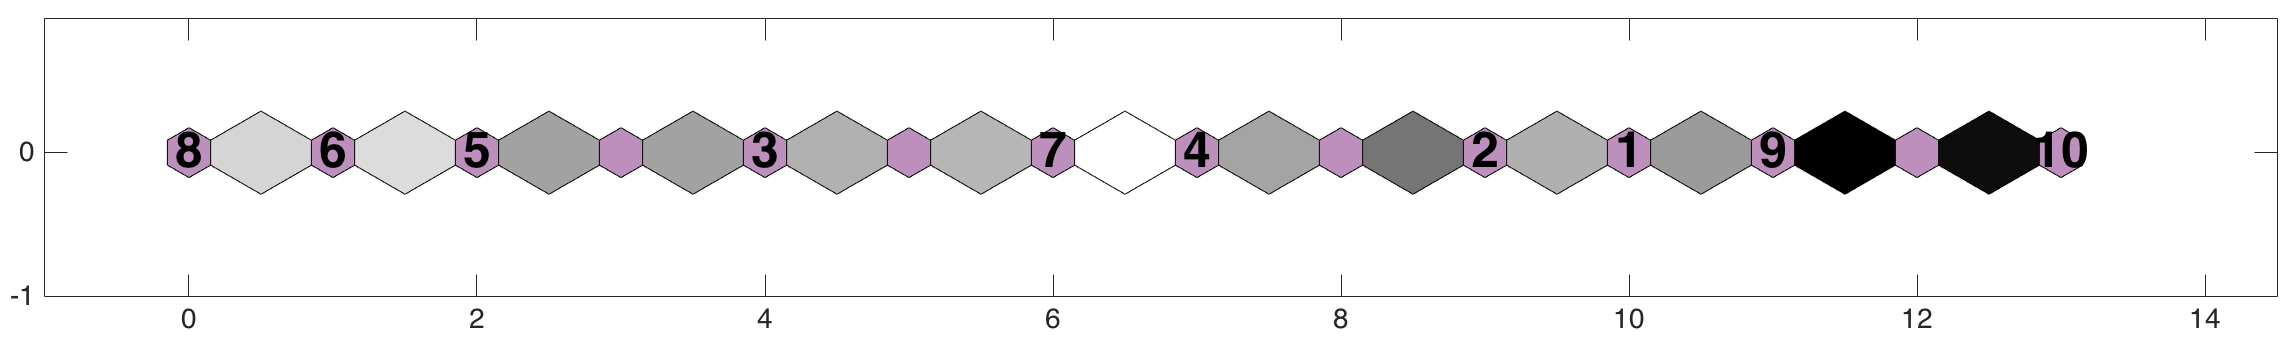
\includegraphics[width=\textwidth]{../image_paper3/images0.01/M31/1D/combine_1D_1by14_all.png}
        \caption{$1\times14$~network}
        \label{fig: M31_net_1by14}
    \end{subfigure}
   \caption[One-dimensional self-organizing map of M31 data]{SOM of the M31 data from $1\times2$, $1\times3$~and $1\times14$~grids. The axes show the position of the neurons. The purple hexagonal shapes represent the neurons. The grey scale colours show the differences between weight of the neurons, with white as the minimum difference and black as the maximum. The numbers in the plot show the M31 regions located in each neuron.}
   \label{fig: M31_nets_1d}
    \end{figure}
    

        %%Network 1by14
        The network with 14 neurons, in Fig.~\ref{fig: M31_net_1by14}, is the first network that has no neuron occupied by more than one M31 region.
        In a larger-grid SOM, the network pays more attention to smaller details and differences in the input data.
        Therefore, since at least 14 neurons are needed to separate all 10 regions in M31, we can conclude that some of the regions have very small differences.
        Regions that are located in similar areas (e.g. spiral arms, bulge, and 10 kpc ring) in M31, like regions 7 and 4 (see Fig.~\ref{fig: regions in m31}), are most likely to have more similarities with each other.
        In Fig.~\ref{fig: M31_net_1by14}, the right-most neuron is occupied by region 10.
        Two black colours between this region and the others indicate the large differences between this neuron and the other ones.
        Region 10 is located in the bulge of M31, and is physically separated from the other regions, which are mostly located around the inner or outer rings.
        The SOM shows that this region has completely different input values from the others: most of the values for region 10 are much higher than for the other regions, which is the main reason for its isolation.
        Region 8 occupies the left-most neuron in this network, suggesting that this region has the most differences from region 10.
        
    \subsection{Inside the Two Neuron Network}
        \label{sec: inside_the_2_neurons}
        Using self-organizing maps, we can identify hidden subgroups in our samples. 
        Each of these subgroups separates for a reason.
        This reason can vary from having higher values in some specific properties, as discussed in Section~\ref{Sec: 1d_cluster}, to some unknown correlations between data that cannot be seen in other groups or in the galaxy as a whole.
        To investigate the latter, we show in Fig.~\ref{fig: cor_cluster1} the Pearson correlation coefficients for the inputs from regions 3 to 8, which were clustered together in the $1\times2$ and $1\times3$ networks (see Figs.~\ref{fig: M31_net_1by2} and ~\ref{fig: M31_net_1by3}).
        
        \begin{figure}
        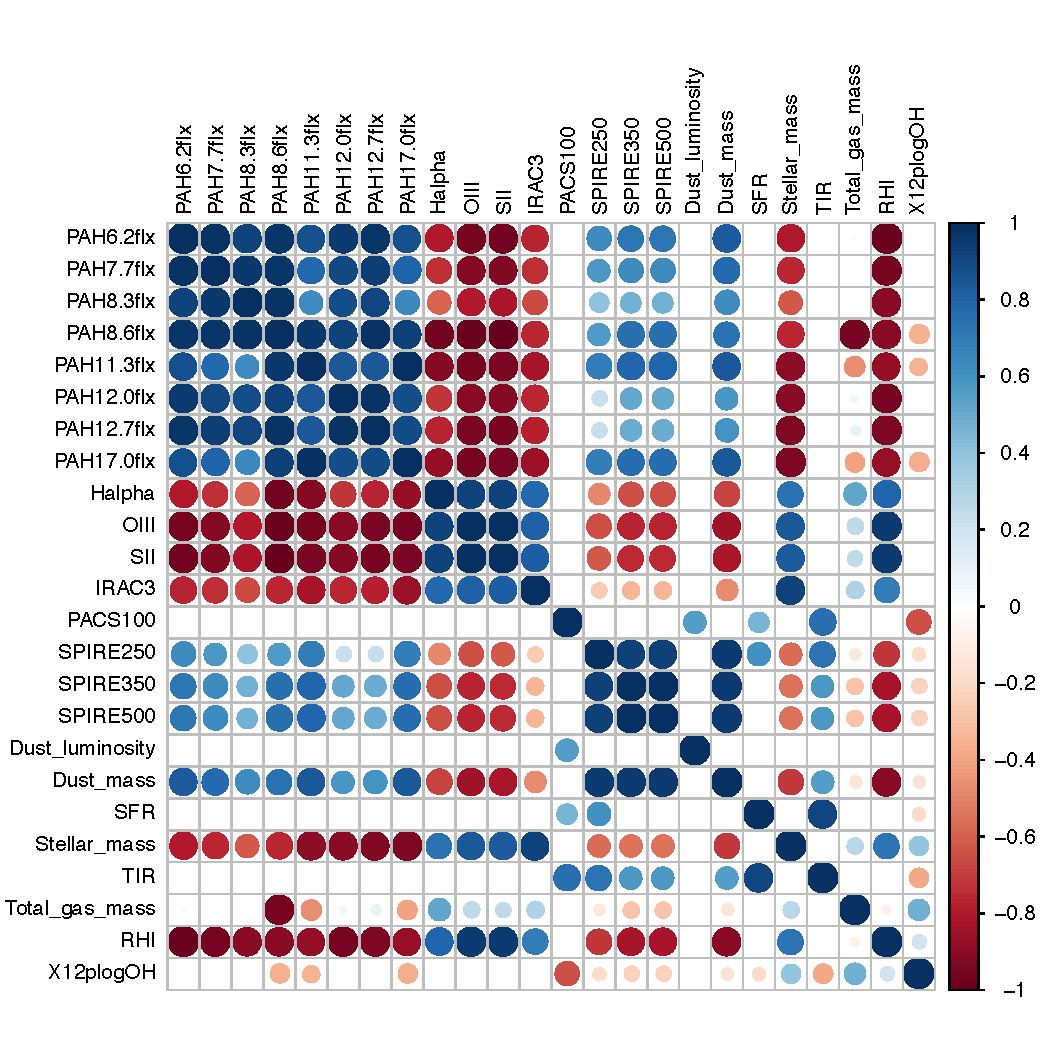
\includegraphics[width=\textwidth]{../image_paper3/images0.01/cor_plots/M31_derived_3_to_8_core_plot_for_paper.pdf}
        \caption[Pearson correlation coefficients for data from the clustered regions in M31]{Same as Fig.~\ref{fig: cor_all}, but here we used data from regions grouped in the left sides of Figs.~\ref{fig: M31_net_1by2} and ~\ref{fig: M31_net_1by3}.}
          \label{fig: cor_cluster1}
        \end{figure}
        
       
        Comparing the correlation coefficient plots for all 10 regions in M31 (Fig.~\ref{fig: cor_all}) and for the clustered data (Fig.~\ref{fig: cor_cluster1}) shows the differences between all 10 regions and clustered data and why regions 3 to 8 become separated from the other regions.
        The main features that differentiate these two plots are the anti-correlations between PAH features and RHI, stellar mass, \halpha, \sii, \oiii, and IRAC~5.8~$\mu$m~emission.
        Additionally, for the PAH fluxes in Fig.~\ref{fig: cor_cluster1}, there are no significant correlations with PACS~100~$\mu$m, L$_\mathrm{dust}$, L$_\mathrm{TIR}$, SFR, or metallicity.
        The PAH fluxes correlate with the SPIRE emission, but to a lesser extent than for the data from all regions.
        
        \cite{Calzetti10} mentioned that with increasing RHI in regions, metallicity and PAH equivalent widths decrease. 
        \cite{Dim15} investigated the correlation between PAHs features and both metallicity and RHI using the equivalent width of the 8~$\mu$m (combination of 7.7, 8.3, and 8.6~$\mu$m components) and the 7.7 and 11.2~$\mu$m features.
        They did not see any relations between PAHs and metallicity or RHI for 10 regions in M31.
        In Fig.~\ref{fig: cor_all}, we show that all the PAH fluxes correlate with metallicity, and PAH fluxes in the 7.7, 8.3 and 17.0~$\mu$m bands weakly anti-correlate with RHI.
        However, in Fig.~\ref{fig: cor_cluster1}, there is no correlation between the PAH fluxes and metallicity, but all of them strongly anti-correlate with RHI.
        \cite{Dim15} argued that the absence of (anti)-correlation between the PAH features and metallicity and RHI was related to a lack of data in low-metallicity regions.
        Although data from more regions would improve the results, our analysis shows that clustering data would show the missing (anti)-correlations.
        For example, for both clusters in Fig.~\ref{fig: M31_net_1by2},
        we can see anti-correlations between PAHs and RHI, but each of them has a different slope which removes the anti-correlation over all 10 regions. 
        
        Correlations between PAH features and SFR, and L$_\mathrm{TIR}$ are well-studied~\citep[e.g.][]{Peeters04,Tielens08}. 
        Many groups have used PAH features as a tracer of SFR by finding correlations between 
        PAH emission and SFR derived from extinction-corrected \halpha~\citep[e.g.][]{Calzetti07,Khramtsova13,Shipley16}.
        These correlations are seen in Fig.~\ref{fig: cor_all}, when we considered the data from all regions, but not in Fig.~\ref{fig: cor_cluster1} when considering the clustered data.
        Note that, since there are only 6 regions in the clustered data, even one outlier in the data may cause the correlation coefficient to become insignificant.
        Further analyses show that the absence of correlations between PAH fluxes and SFR is because of one outlier: region 6. Region 6 is located in a FUV-bright region, which breaks the correlations. 
        When we disregard this region, high correlations between 6.2 to 17.0~$\mu$m~PAHs and SFR (and L$_\mathrm{TIR}$) reappear.
        
     
        Strong anti-correlations between 6.2 to 17.0~$\mu$m~main PAH features and RHI, stellar mass, \halpha, \sii, \oiii, and IRAC~5.6~$\mu$m~emission in Fig.~\ref{fig: cor_cluster1} were not seen in Fig.~\ref{fig: cor_all} (even if we ignore the outlier values).
        Anti-correlations between PAH features and the \halpha, \sii, and \oiii~emission could be the result of one of the following. 
        First, the optical data are not corrected for dust extinction.
        The PAH features correlate with the amount of dust while \halpha~emission anti-correlates with the amount of dust due to extinction as suggested by \cite{Calzetti94}.
        Therefore, higher PAH fluxes imply higher dust abundance and less \halpha~emission, and the same holds for \sii~and \oiii~emission.
        Second is the possible effect of the structure of the observed regions.
        If the observed regions are located near the edge of \hii~regions we would expect to see more PAH and less \halpha~emission. 
        The anti-correlations between 6.2 to 17.0~$\mu$m~PAH features and RHI have been seen in other studies, as well~\citep[e.g.][]{Wu06, Gordon08,Calzetti10,Dim15}. 
        \cite{Wu06} suggested these anti-correlations could be the result of PAH destruction due to a high amount of harder radiation (thus higher RHI).
        On the other hand,~\cite{Gordon08} argued that the harder radiation could make the photodissociation regions (PDRs) smaller.
        The PAH features are mostly coming from the PDRs that are surrounded by \hii~regions, and the PAH features' underlying continuum emission is from the \hii~regions.
        Therefore, the lower flux of the PAH features could be the result of the smaller size of PDRs.%Els: If you have an harder radiation field, you destroy your smaller PAHs. Hence, simply a harder RHI does not argue for a smaller PDRs being more plausible. 
        The latter reason, which could also describe the anti-correlation between PAH features and \halpha~emission, seems to be the more probable one. 
        
        The strong anti-correlation between PAHs and stellar mass suggests that, a higher stellar mass decreases PAH emission. 
        In observations of M33,~\cite{Calapa14} showed that the 8/250~$\mu$m luminosity ratio correlates with 3.6~$\mu$m emission, which translates to stellar mass, %Els: I'm unfamiliar with the details of this translation. But if you look at individual HII regions or starforming complexes, I would think that the 3.6um flux is not dominated by the stellar light as the stars are too hot to have a large fraction of emission at these wavelengths?
        and conclude that the PAH emission traces the old stellar population.
        In Fig.~\ref{fig: cor_cluster1}, we see a weak anti-correlation between SPIRE 250~$\mu$m emission and the stellar mass.
        We see no correlation between 8/250~$\mu$m luminosity and stellar mass, either in the clustered data or in all 10 regions.

        To test that whether the anti-correlation between stellar mass and PAH emission is the result of the destruction of PAHs in high stellar mass regions, or that high stellar mass obscures PAH emission, we compared PAH abundance with stellar mass for the clustered regions.
        The ratio of 8/24~$\mu$m emission, which can be considered as a proxy for PAH abundances~\citep[e.g.][]{Sandstrom10,Khramtsova13}, does not anti-correlate with stellar mass for either the clustered data or all 10 regions.
        Therefore, we conclude that in our sample, stellar mass does not cause the destruction of PAHs.
        
        The anti-correlation between stellar mass and PAHs could be result of the position of the regions within M31.
        Regions 5, 6, and 8 are located in the stellar disk of the galaxy and have relatively high stellar mass and faint PAH emission. 
        According to~\cite{Dim15}, regions 5 and 8 are the only two regions in thesample that do not include an \hii~region, which could be the reason for the faint PAH emission for these regions.
        Regions 4 and 7 have similar quantities for both stellar mass and PAHs and region 3 has high PAHs and low stellar mass.
        Without data from more regions in M31, we cannot confidently say that higher stellar mass decreases PAH fluxes.
        
        
       Regardless of the fact that some of the (anti)-correlations in Fig.~\ref{fig: cor_cluster1} might have physical meaning, we have to mention that we only used 6 regions to calculate these correlation coefficients.
       The number of data points is not high enough to yield a strong conclusion about PAH properties in M31.
       However, we can conclude that since the correlation coefficients derived from the clustered data (Fig.~\ref{fig: cor_cluster1}) differ from the correlation coefficients derived from the data from all 10 regions (Fig.~\ref{fig: cor_all}), the SOM separated a hidden cluster of the data which has different properties.
        
        
        
 %----------------------------------------------------------------------------------------
%----------------------------------------------------------------------------------------
%----------------------------------------------------------------------------------------
%Result Part 2: 2D SOMs
%----------------------------------------------------------------------------------------
%----------------------------------------------------------------------------------------
%----------------------------------------------------------------------------------------
\section{Two-Dimensional Self-Organizing Maps}
 \label{sec: 2d_cluster}
    Although 1D networks are helpful to give a general idea about the data, neurons in 1D maps have a maximum of two neighbours, which can limit the usefulness of the results.
    In 2D networks, each neuron has two to six neighbours, which allows them to capture a complete picture of the complicated relations in the input data.
    Accordingly, we created $10\times10$ 2D networks to study the data in detail.
    As mentioned in previous sections, the sizes of SOMs are arbitrary and must be decided by users based on their goals for use of the SOM.
    
    In this section we chose $10\times10$ size despite knowing, from the size of our input data, that most of the neurons would be empty.
    Using 2D networks, we are mostly interested in the ability of the SOMs to show the underlying structure of the data rather than its clustering features.
    Fig.~\ref{fig: all_derived_ones} shows the 2D SOM of the M31 data.
    Similar to Fig.~\ref{fig: M31_net_1by14}, all the 10 regions are completely separated from each other in Fig.~\ref{fig: all_derived_ones}.
    In Fig.~\ref{fig: all_derived_ones}, all the regions except regions 4 and 7 are surrounded by white colours.
    This indicates that all the immediate neighbours for neurons occupied with each region have similar properties as the occupied ones, except for regions 4 and 7.
    These two regions are sitting in very close regions and their smallest dissimilarity causes the changes in distances between their neighbours.
    \import{../image_paper3/text_files/image_texts/}{all.tex}
    
    Regions 4 and 7 are in the top left of Fig.~\ref{fig: all_derived_ones} with a very bright colour between their neurons, indicating that these two regions are very similar.
    Considering the position of these two regions in M31 (both right on the edge of the star forming rings in the galaxy), similarity of these two regions was predictable.
    The position of region 3 on the SOM is relatively close to the position of regions 4 and 7, but with a darker colour between the nodes. 
    In Fig.~\ref{fig: regions in m31} it is clear that this region in M31 is physically closer to regions 4 and 7 than to any other region, but it is on the outer side of the star forming ring.
    Regions 5 and 6 are in the second neighbourhood (there are two neurons between them) of the SOM, with a medium gray colour between them.
    These two regions are physically located around the inner ring of the galaxy.
    Regions 8 and 6 are both in the inner ring of M31, but region 6's location has more star formation, which could be the main reason for their relative distance in the SOM in Fig.~\ref{fig: all_derived_ones}. 
    
    Regions 1 and 9 are close to each other and in the same side of the star forming ring. 
    However, region 1 is in an area of the galaxy with less diffuse \halpha~emission than region 9, which might be the reason for their distances in the SOM.
    Region 2 is more distant from other regions in the galaxy and located in the star forming ring.
    However, similar to regions 1 and 4, region 2 is located in an area of the galaxy with less diffuse \halpha~emission.
    Therefore, the place of region 2 in the SOM tends towards regions 1 and 4. 
    Region 10 is in the bulge of the galaxy, and its position on the SOM is isolated from all the other regions by a strip of a dark colours. 
    
    In order to analyse effects of any input data on the final SOM, in the following we created SOMs from various subsets of data.
    We compare results of the subsets with one another and with the SOM created from all data in Fig.~\ref{fig: all_derived_ones}.

    \subsection{Subsets}
    \label{sec: subsets}
    
            For analysing subsets, we create SOMs by using only PAH data, as well as using all data except the PAHs (Fig.~\ref{fig: PAHS_or_not_PAHs}).
             \import{../image_paper3/text_files/image_texts/}{PAHS_or_not_PAHs.tex}
            Comparing the SOM from all data in Fig.~\ref{fig: all_derived_ones} with the SOMs in Fig.~\ref{fig: PAHS_or_not_PAHs} shows that the general position of almost all regions in those networks are the same. 
            Region 10 is in one corner of all three networks.
            However, in Fig.~\ref{fig: all_derived_ones} and Fig.~\ref{fig: wt_pahs}, region 10 is isolated from the other regions, while in Fig.~\ref{fig: only_pahs}, region 10 is much less isolated and only shows complete dissimilarity with region 8.
            Regions 9 and 10 are totally isolated in the SOMs in Fig.~\ref{fig: wt_pahs}, but in Fig.~\ref{fig: only_pahs}, they are more similar to other regions.
            In both SOMs in Fig.~\ref{fig: PAHS_or_not_PAHs}, there are dissimilarities between regions in M31 but in Fig.~\ref{fig: wt_pahs}, the colours are much darker than the ones in Fig.~\ref{fig: only_pahs}.
            This indicates that there is more similarity between the PAH features over all 10 regions than between the other input data.
            
            We increased the dimension of input data in Fig.~\ref{fig: only_pahs} (PAH-only data) gradually, by adding other quantities to the input data. 
            The order in which data were added is the same as the order in Fig.~\ref{fig: cor_all}, i.e. the SOM in Fig~\ref{fig: col3and11_dist} was created from PAH and \halpha\ emission as input data, the SOM in Fig~\ref{fig: col3and12_dist} created from PAHs, \halpha~emission and \sii~ continuum, and so on. 
            \import{../image_paper3/text_files/image_texts/}{col3byall.tex}
            
            At the beginning of each run, the SOM algorithm assigns a random weight to neurons that causes the overall position of regions in networks (even with the same input data) changes in each run of the algorithm.
            However, the position of each region relative to other regions changes dramatically only when the new sets of input data are given to the algorithm (assuming all the initial values for the run are unchanged).
            In all SOMs in Fig.~\ref{fig: inc_D_col3s}, region 10 is located in the corner of the SOMs, but in  Figs.~\ref{fig: col3and11_dist},~\ref{fig: col3and14_dist},~\ref{fig: col3and17_dist},~\ref{fig: col3and21_dist}, and ~\ref{fig: col3and22_dist}, it is placed in the left side of the SOMs and in the others it is in the right side of the networks.
            In our discussion on differences between networks, we do not address the changes in the network due to initialization of the SOM algorithm and only consider the effect of changing the input data.
            
            Comparing Figs.~\ref{fig: col3and11_dist} to~\ref{fig: col3and25_dist} shows that adding \halpha~emission data to PAH features causes regions 9 and 10 become isolated. 
            Increasing the dimension of the input data makes region 10 more isolated.
            The relative positions of regions 4 and 7 stay the same with increasing the dimensions of the input data. 
            Adding SPIRE 350, 500~$\mu$m emission and L$_{\rm dust}$ does not have any obvious effect on the networks.
            Stellar mass, total gas mass, dust mass and RHI data alternate the distances between neurons effectively, but it seems that adding SFR, L$_{\rm TIR}$ and metallicity data revokes those changes.
            
            We generated other subsets of the data based on the results in Fig~\ref{fig: inc_D_col3s} to further study the effects of the input data on SOMs.
            Subset 1, listed in Table~\ref{tab: subset1}, includes all the input data except stellar mass.
            Table~\ref{tab: subset5} lists data used in subset 2, which includes all data except that the PAH fluxes are combined into a total PAH flux. 
            For subset 3 (in Table~\ref{tab: subset6}), SPIRE 250 and 500~$\mu$m were removed from subset 2.
            Figs.~\ref{fig: subset1} --~\ref{fig: subset6} show SOMs created by data from subsets 1 to 3, respectively.
            The remaining subsets are discussed in Appendix~\ref{sec: app_2d_soms_SOMN}.

            The results from Table~\ref{tab: subset1} are used to create the network in Fig.~\ref{fig: subset1}. 
            In this SOM, compared with the SOM from all the data in Fig.~\ref{fig: all_derived_ones}, regions 1 and 9 are closer to region 10. 
            Regions 1 and 9 are the ones with lowest stellar mass values, and region 10 has the highest stellar mass value among those 10 regions. 
            Since the difference in the amount of stellar mass was one of the most distinct differences between these three regions, removing stellar mass from the input data reduced the distance between these regions.
            Regions 5, 6 and 8 have the same relative distance from each other as in Fig.~\ref{fig: all_derived_ones}, but they are all closer to the position of region 10.
            The distance between regions 2 and 3 is reduced but in the meantime the colour between them became darker.

            \import{../image_paper3/text_files/tables/}{subset1.tex}
            \import{../image_paper3/text_files/image_texts/}{subset1.tex}

            Changing from separate values for each PAH features to a single value for the total PAHs caused small changes to the SOM map in Fig.~\ref{fig: subset5} compared to the one in Fig.~\ref{fig: all_derived_ones}. 
            The distance between the positions of regions 6 and 8 increased significantly, while the position of region 2 moved closer to the positions of regions 4 and 7.
            The winner neurons for regions 3 and 5 moved towards each other, but the colours between them became much darker. 

            \import{../image_paper3/text_files/tables/}{subset5.tex}
            \import{../image_paper3/text_files/image_texts/}{subset5.tex}

            Fig.~\ref{fig: subset6} shows the SOM generated from data listed in Table~\ref{tab: subset6}, which includes all the data from Table~\ref{tab: subset5} except for  the SPIRE 250 and 500~$\mu$m emission.
            Although for most of the regions we see the changes in their positions, the colours between neurons change as well. 
            The distance between the positions of the regions 4 and 2 is increased as are the
            distances between regions 7, 3 and 6.
            In both cases, SPIRE 250 and 500~$\mu$m emission of these regions are similar to one another, and removing these two parameters from the input data moved the positions of the regions further from each other. 
            \import{../image_paper3/text_files/tables/}{subset6.tex}
            \import{../image_paper3/text_files/image_texts/}{subset6.tex}
            
            Subsets, as studied in this section, can be used to learn about the effect of each input on the SOM and tell us about variation in the input data.
            Comparing Fig.~\ref{fig: only_pahs} with other networks show us that PAH features are less variable than other input data.
            These result is consistent with results from~\cite{Draine14}, who showed that the amount of PAHs in M31 for regions within 20~kpc radius is constant.
            Additional evidence for the PAH features varying significantly less than other parameters is that changing from the PAH single band emission to total PAHs does not affect the networks.
            In contrary, PACS~100~$\mu$m, stellar mass, total gas mass and RHI
            are the data with the most variance; adding them to input data increases the dark colours between neurons significantly.
            Although with changing input parameters for each network the distances between neurons and positions of the regions change, the general positions of the regions relative to one another does not change dramatically.
            Therefore, the networks created by subsets can be used to predict the properties of unobserved quantities in other regions of the galaxy.
            For example, photometry data, stellar mass, SFR, L$_\mathrm{dust}$, L$_\mathrm{TIR}$, and dust mass are available for most of M31. 
            The network from Fig.~\ref{fig: wt_pahs} can be applied to 
            these data from another region in M31.
            By comparing the position of the new region (with the same spatial size of these 10 regions) with respect to our original 10 regions in the network, one would have an estimate for total PAHs in the new region without having any observational data for it.


    \subsection{Applying Networks to M101 Observations}
    Another application of self-organizing maps made with data from a single galaxy is to apply its trained networks on data from other galaxies to make predictions.
    To demonstrate this, we generated an SOM using only M31 measurements which were also available for M101 (Fig.~\ref{fig: subset9}a). 
    \cite{Dim15} compared PAHs in M31 with those from \hii~regions in M101, and showed the similarity between PAHs in these two galaxies (for more detail see \cite{Dim15} and \cite{Gordon08}).
    In order to test whether these similarities are limited to PAH features or can be extended to other features in these two galaxies, we applied the SOM created using M31 data in Fig.~\ref{fig: subset9}a to M101 data (Fig.~\ref{fig: subset9}b).
    Since the neurons in the SOM network created by M31 data already have their finalized weights, the algorithm finds the minimum differences between parameters for each region in M101 and the weights of neurons and introduces the winner neuron in one iteration.
    
    In the SOM that is created by M31 data in Fig.~\ref{fig: subset9}a, as in the others, region 10 is separated from other regions in M31.
    Regions 7 and 4 are close to each other with very light colours between their neurons, and as in the other SOMs regions 6, 8, and 5 are close to each other, but with medium dark colour between them.
    Given the fact that we know the relative relation between M31 regions from 2D networks, we can analyze properties of M101 regions from their locations in Fig.~\ref{fig: subset9}b.
    To do so, we compared positions of regions in M31 and M101 in the networks presented in Fig.s~\ref{fig: subset9}a and~\ref{fig: subset9}b, respectively, and based on colours between regions determine their (dis-)similarities.
    \import{../image_paper3/text_files/image_texts/}{subset9.tex}
    
    Region 5 in M31 and region 8 in M101 and regions 6 in M31 and region 2 in M101 occupy neurons with a white colour between them in the network in Fig.~\ref{fig: subset9}, which immediately suggests that these regions have similar properties. 
    Region 2 in M101 is a bright \hii~region located at the end of  one of the M101 spiral arms (see Fig.~\ref{fig: regions in m101}) while
    region 6 in M31 is located near the inner star-forming ring (see Fig.~\ref{fig: regions in m31}).
    Both regions have relatively low PAH emission and a median amount of  SFR compared to other regions in the galaxy, making them very similar.
    
    Region 5 in M31 is in the inner ring of the galaxy and it is one of two regions in M31 that is not an  \hii~region, while
    region 8 in M101 is in a spiral arm of the galaxy.
    Relatively low stellar mass, SFR and SPIRE band emission caused these two regions to be nearby in the map.
    In Section~\ref{Sec: 1d_cluster} we showed that regions 3 to 8 in M31 have similar properties; in Fig.~\ref{fig: subset9}b we see that regions 1 to 3 and 5 to 8 in M101 are located near regions 3 to 8 in M101. 
    These regions all have medium or low PAH emission, dust and SFR compared to the remaining regions.
    
    Region 7 in M101 is located in the nucleus of the galaxy and has relatively higher values of the quantities than the other regions.
    This region is located in the top right side of the network in Fig.~\ref{fig: subset9}, close to the location of M31 region 10 in the network.
    Since the bulge of a spiral galaxy has a different environment from its nucleus, region 7 in M101 and region 10 in M31 do not occupy the same neuron in the SOM, and have a medium grey colour between their neurons.

    Region 1 in M101 is also located near the nucleus of M101 (see Fig.~\ref{fig: regions in m101}), but has considerably lower values in all the quantities compared to region 7.
    The lower values for fluxes of the PAH features and moderate amount of the SFR caused this region to be placed between M31 regions 4 and 5 in the network. 
    Fig.~\ref{fig: subset9}b shows that region 4 in M101 is separated from other regions and located between M31 regions 9 and 10.
    \cite{Gordon08} showed that this region is a diffuse nebula in M101, with high PAH emission. 
    This region also shows a high SFR and stellar mass, explaining why the location of M101 region 4 in the SOM is close to that of M31 regions 9 and 10.
    
    Knowing the effects of the different input quantities on the networks from Section~\ref{sec: subsets}, can yield ideas about data entry from other regions/galaxies.
    In this section we showed that we can use networks that are created by data from nearby galaxies to study the properties of other galaxies.
    If an SOM network is available, applying data from other regions to the network is very time efficient to learn about relative properties of galaxies.
    We should note that, since we normalized data before using them in the networks, we only see relative properties of the regions.
    Therefore, we need data from at least a few regions in the galaxy to use this application of SOMs and cannot use these networks to learn about properties of a single region in other galaxies.
    As mentioned before, since we know the properties of regions in M31, from Fig.~\ref{fig: subset9}, we can quickly conclude that region 7 and 4 have relatively higher surface brightness than the other regions in M101. 
    Similarly, we can say that regions 6 and 8 in M101 have very faint surface brightness for most of the parameters, and are very different from regions 7 and 4.
    
    
    
%----------------------------------------------------------------------------------------
%----------------------------------------------------------------------------------------
%----------------------------------------------------------------------------------------
%Summery
%----------------------------------------------------------------------------------------
%----------------------------------------------------------------------------------------
%----------------------------------------------------------------------------------------
\section{Summary}
\label{sec: summary}

We present the results of studying spatially resolved regions in nearby galaxies using Kohonen self-organizing maps.
Self-organizing maps both cluster data and show relative distance between the clusters. 
We utilized the method to find hidden subgroups in the data as well as to find relations between those groups.

Using smaller-sized self-organizing maps, we clustered M31 data into two major groups, which led us to correlations that could not have otherwise been seen without clustering.
Six of the regions in M31 create a subgroup with relatively lower mid- and far-infrared emission.
PAH fluxes in these regions are highly anti-correlated with \halpha, \sii, \oiii~and IRAC 5.8~$\mu$m emission, stellar mass and radiation hardness index.
These anti-correlations are insignificant when the full dataset is considered.
The most probable reason for PAHs to anti-correlate with optical emission lines and RHI is a harder radiation field.
This makes the size of \hii~regions bigger and the size of photo-dissociation regions smaller, causing more \halpha~emission and less PAH emission, respectively.

PAHs in clustered data also show an anti-correlation with stellar mass.
We discussed the possibility that higher stellar mass might destroy PAHs;
however, we did not find any correlation between 8/24~$\mu$m emission, as a tracer of PAH abundance, and stellar mass.
Unlike previous studies, we also did not find any correlation between 8/250~$\mu$m emission and stellar mass. 
This result shows that PAHs in the clustered regions in M31 are not heated by the old stellar populations.
The reason behind the observed anti-correlation between PAH features and stellar mass needs further investigation, which requires mid-infrared PAH observations for more regions in M31. 

In self-organizing maps with larger sizes, networks can be used to illustrate the relations of the regions with one another.
We found the relative similarity between M31 regions by varying the size of the networks.
A one-dimensional network with 14 neurons was needed in order to
separate all 10 regions; some of the regions in M31 (e.g. regions 4 and 7) have very similar properties.
Two-dimensional networks provide us with a more complete picture of the data.
We created various subsets of the input data and generated different networks which helped to show relations between regions in M31 more clearly.
Region 10, which is located in the bulge of M31, always becomes isolated in the networks, except when we  used only PAH data to create a network.
In that network region 10 blends more with the other regions and is only differentiated from region 8, which is located inside the inner ring of M31.
These results suggest that the PAHs in all 10 regions have almost the same properties.

We introduced self-organizing maps as a method that can be used to predict various quantities based on the relative positions of the regions in the networks.
For regions that lack the observational data for some quantities (e.g. PAH emission), SOMs can be used to extrapolate the unobserved quantities.
Applying the SOMs from M31 to observations of M101, we found regions with similar properties in both galaxies placed in close regions in the SOMs.
Using this ability of the SOM, we can predict properties of regions in other nearby galaxies very quickly.

The networks we created used values for 26 quantities from 10 regions in M31, which is not a large sample.
Increasing the dimension of the data and the number of regions would yield more reliable networks.
Since there is very little spatially-resolved PAH spectroscopy for other galaxies from the \Spitzer Space Telescope, increasing the size of samples will require data from the James Webb Space Telescope.
The method described in this work can be used to select target regions for PAH observations with that facility. 


%----------------------------------------------------------------------------------------
%----------------------------------------------------------------------------------------
%----------------------------------------------------------------------------------------
%biblio
%----------------------------------------------------------------------------------------
%----------------------------------------------------------------------------------------
%------------------

\addcontentsline{toc}{section}{Bibliography}
\bibliographystyle{apj.bst}
\bibliography{ref_paper3.bib}
\chapter[Classifying High-Redshift Galaxy Spectra]{Clustering galaxy spectra at $0.5<z<1$: an unsupervised approach}
\label{ch: paper2}
\defcitealias{Hossein12}{T12}
\defcitealias{Kinney96}{K96}
\defcitealias{Noll09}{N09}

%----------------------------------------------------------------------------------------
%----------------------------------------------------------------------------------------
%----------------------------------------------------------------------------------------
%Intro
%----------------------------------------------------------------------------------------
%----------------------------------------------------------------------------------------
%----------------------------------------------------------------------------------------
\section{Introduction}
\label{sec: intro_somz}
%General information about SEDs
Nearly all information we can obtain from a galaxy is encapsulated in the light it emits; every observable phenomenon in a galaxy leaves a footprint on its spectral energy distribution (SED).
We can determine some physical property of a galaxy by properly modeling various features observed in its SED, and the general shape of the SED can be used as an identifier of the morphological type.
Considering the main features of SEDs, galaxies can be categorized into two main groups: elliptical or spiral. %PB: quiescent or SB?
Each group has its own characteristic features and can in turn be divided into many sub-branches.

%%Creating templates and NIR_UV templates
Several attempts have been made to create a complete set of templates for categorizing the spectral type of galaxies using data from nearby galaxies~(e.g.~\citealt{Kinney93}, \citealt[][hereafter \citetalias{Kinney96}]{Kinney96}, \citealt{Bershady00}, \citealt{Mannucci01}). 
Based on their usage, these templates are restricted to certain wavelengths.
In near-infrared (NIR) to ultraviolet (UV) wavelengths (the region where energy output of stars peaks), the SED contains information about the main physical properties of galaxies, e.g., age, star formation rate (SFR), stellar mass, metallicity, and interstellar medium.


% categorizing galaxies based on their SED

Advances in techniques and detectors have resulted in more detailed observations of SEDs and also made classification of galaxies more complex.
Since no two galaxies, even with the same morphology, have exactly the same properties, classifying SEDs of galaxies using templates is very challenging.
To overcome this challenge, many fitting methods have been developed and used to find template matches for SEDs, with $\chi^2$ minimization being the most commonly used. 
Artificial neural networks, K-means clustering, and principal component analysis are some other methods used to cluster and classify spectral types of galaxies \citep[e.g.][]{Allen13,Ordov14,Shi15}.

%ANNs
Artificial neural networks (ANNs), which are inspired by the way neurons in a human brain route and process data, are very powerful tools that are used in data processing and pattern recognition problems.
An ANN contains many interconnected units (nodes or neurons) which process data and work together to solve problems.
It uses a set of training methods to learn about nonlinear and complex relations between input and output data, and how to apply these relations to new sets of data~\citep[e.g.][]{Hossein14,Hossein16,Ellison16a, Ellison16b}.
Studies have shown that ANNs outperform chi-square minimizing techniques and can be used as an alternative choice for fitting data~\citep[e.g.][]{Marquez91}.
Specifically, ANNs perform faster in large databases~\citep[][]{Gulati97}.

%Training methods for networks
Neural networks can be trained using two methods: supervised and unsupervised.
In supervised method, a neural network would be trained using input data based on a desired outcome.
This method is very useful for classification of data with specific target values.
On the other hand, in unsupervised method there is no prediction of output.
This method classifies data based on their underlying structures and hidden patterns.
The unsupervised method is very helpful to obtain knowledge from the data, or when the underlying structure of data is not well established.

%SOM
A Kohonen self-organizing map (also called self-organizing map, or SOM) is an unsupervised neural network for mapping and visualizing a complex and nonlinear high dimension data introduced by~\citet{Kohonen82}.
It shows simple geometrical relationships in non-linear high dimensional data on a map \citep{Kohonen98}.
%SOM in Astronomy
The utilization of the SOM in astronomy dates back to the 1990s, with \citet[][]{Odewahn92}, \citet[][]{Hernandez94}, and \citet[][]{Murtagh95} among the first to use SOMs in their studies.
\citet{Geach12} used COSMOS data to demonstrate two of the main applications of SOMs: object classification and clustering, and photometric redshift estimation. The latter has been the subject of many other studies \citep[e.g.][]{Kind14a}.
From classifying quasars' spectra to star/galaxy classifications, from gamma-ray burst clustering to classification of light curves, this method has proved to be useful in various fields of astronomy \citep[e.g.][]{Maehoenen95, Miller96, Andreon00, Balastegui01, Rajaniemi02, Brett04, Scaringi09}.


%SOM in Astronomy continued.
Large spectroscopic surveys have made available integrated spectra of millions of galaxies.
These integrated spectra combine the light of billions of individual stars and nebulae within a galaxy, and
finding patterns and common characteristics between galaxies can be a complex task.
\citet{In12} introduced a new clustering tool based on the SOM method for analyzing these large datasets.
They used $\sim 60000$ spectra from the Sloan Digital Sky Survey \citep[SDSS;][]{Abazajian09} to test their tool, and created very large SOMs to analyze the type of spectra/objects.
They also generated SOMs from quasars' spectra in order to find unusual types of spectra. 
Later, \citet{Meusinger16} used these SOMs and updated data from SDSS and other surveys to find a new class of quasars.
The other application of SOMs is to find outliers or errors in the data.
\citet{Fustes13} produced a package based on SOM to classify spectra from the GAIA survey that were previously classified as ``unknown'' by the SDSS pipeline. This package can distinguish an astronomical object from instrumental errors, and then classify the object based on its spectrum.

%What \citetalias{Hossein12} did
~\citet[][hereafter \citetalias{Hossein12}]{Hossein12} classified spectral types of a sample of 142 galaxies using a supervised (Multi-layer feed-forward) neural network method, based on the spectral templates presented by \citetalias{Kinney96}.
With the supervised method, they could only classify spectral types of 105 out of the 142 galaxies.
The spectra of the 37 galaxies from their samples could not be matched with any of those in the \citetalias{Kinney96} templates. 
In order to classify the remaining 37 galaxies, they combined spectra of the \citetalias{Kinney96} templates.
\citetalias{Hossein12} also showed that there are tight correlations between physical properties of galaxies, and these correlations might be different for each type of galaxy.

%What we did
In this paper, we compare supervised and unsupervised methods of galaxy spectral classification directly, using exactly the same data as \citetalias{Hossein12}.  
Our hypothesis was that since a self-organizing map has the freedom to classify objects in between known classes, it could be applied to this data 
to find the best spectral class for the 37 galaxies that could not be classified by the supervised method.
First, we train self-organizing maps using the \citetalias{Kinney96} spectral templates and compare our classification with the \citetalias{Kinney96} classification.
Then, we use the trained network to classify the spectra of 142 galaxies with $0.5 < z < 1$ from \citetalias{Hossein12}. 
As in \citetalias{Hossein12}, we examine the averaged properties of the new galaxy groups and compare them with previous work.
In Section $\S$~\ref{sec: data_highZ}, we present the data that we use to train and test our networks. 
We describe the SOM methods in Section $\S$~\ref{sec: method_somz}. 
The results of the spectral classifications and a comparison with previous studies are presented in Section $\S$~\ref{sec: result}. 
In Section $\S$~\ref{sec: summary_SOMZ}, we summarize our results and discuss potential future work in this subject.
%----------------------------------------------------------------------------------------
%----------------------------------------------------------------------------------------
%----------------------------------------------------------------------------------------
%DATA
%----------------------------------------------------------------------------------------
%----------------------------------------------------------------------------------------
%----------------------------------------------------------------------------------------

\section{Data}
\label{sec: data_highZ}
We use spectral templates from \citetalias{Kinney96} to train neural networks.
To test the trained networks, we use SED and physical properties of 142 galaxies at $0.5<z<1$ from \citetalias{Hossein12}.
Following the \citetalias{Hossein12} work, we chose these two sets of data not only to show the application of SOMs in spectral clustering, but also to easily compare supervised and unsupervised methods.

 \subsection{Kinney Spectral Model}
     \begin{figure}
        \centering
        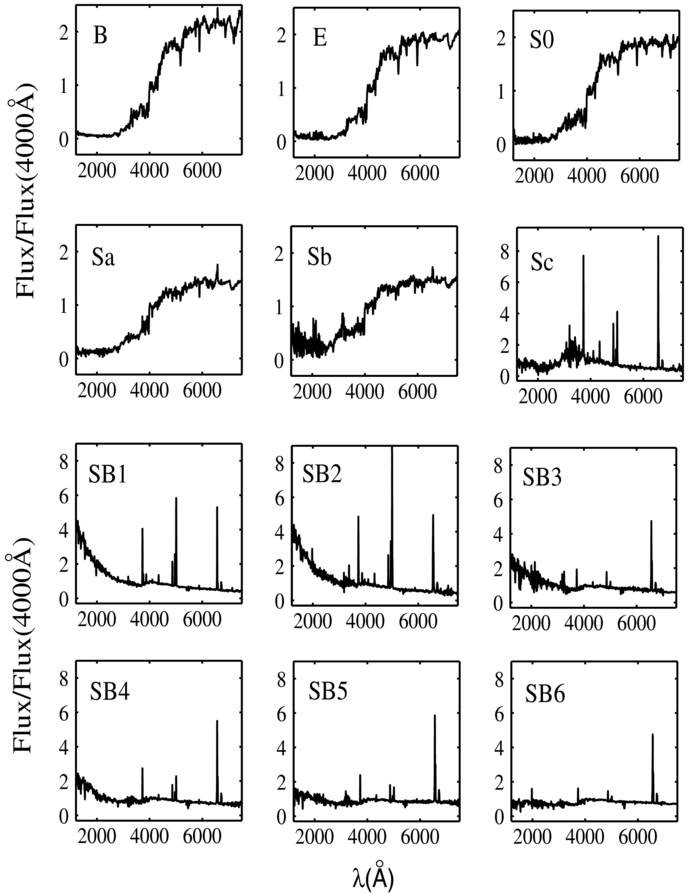
\includegraphics[width=0.9\textwidth]{../image_paper2/k96.jpg}
        \caption[\citet{Kinney96} spectral templates for 12 types of galaxies]{\citet{Kinney96} spectral templates for 12 types of galaxies from \citet{Hossein12} paper (Fig. 1 in \citet{Hossein12}). The type of each template is shown in each frame. Plots B, E, S0, Sa, Sb and SC show spectra that belong to quiescent galaxies. Starburst galaxy spectra are indicated with SB 1 to 6. Higher numbers represent more intrinsic extinction.}
        \label{fig: k96}
    \end{figure}
      
    \citetalias{Kinney96} used ultraviolet-optical spectra of 70 star-forming and quiescent nearby galaxies to produce a set of templates that contained 12 types of spectral templates.
    These templates have been widely used in many studies to determine morphological type of galaxies or properties of specific types of galaxies~\citep[e.g.][]{Shakouri16, Paiano16, Laporte16, Holden16}.
    \citetalias{Kinney96} stated that these templates can also be used to classify the spectra of high-redshift galaxies. 
    
    The 12 templates are divided based on their morphological types for quiescent galaxies or their extinction for starburst galaxies (Fig.~\ref{fig: k96}). 
    The quiescent group of galaxies includes Bulge (B), Elliptical (E), S0, Sa, Sb, and Sc galaxies.
    The bulge group represents galaxies similar to M31 and M81, whose UV and optical spectra are dominated by their bulge stellar populations.
    The starburst galaxies are divided into six groups (SB1 to SB6) based on their intrinsic extinctions ($E(B-V)$). 
    As Fig.~\ref{fig: k96} shows, SB1 galaxies have lower internal extinctions ($E(B-V) \simeq 0.05$), while SB6 galaxies have the highest amount of extinction ($E(B-V) \simeq 0.65$) among starburst galaxies. 
    In the quiescent (B to Sb) templates, the spectrum is redder; strong absorption lines and the 4000~\AA~break are distinguishable.
    SEDs of starburst galaxies are flatter in the optical and near-infrared region than those of the quiescent ones and show strong emission lines.
    For more details on each spectral type, we encourage readers to see \citetalias{Kinney96} and references therein. 
   The \citetalias{Kinney96} spectra span from $\sim1200$~\AA~to $10000$~\AA~with a resolution of $\sim 10$~\AA.
    However, in this work we only use $\sim1200< \lambda < 8000$~\AA~to train our networks; 
    this wavelength range was chosen due to availability of flux information in those wavelengths for all 12 templates. 

 \subsection{SED and Properties of the Sample Galaxies} 
    \citetalias{Hossein12} selected 142 galaxies from the spectroscopic campaign of the ESO GOODS-South field~\citep{Vanzella05, Vanzella06, Vanzella08}.
    The 142 galaxies were selected based on the availability of photometry from HST/ACS, VLA/ISAAC, and {\it Spitzer}/MIPS and IRAC (10--13 filters with $\sim 0.4<\lambda<24~\mu$m in the observed frame).
   Data from these instruments was necessary in order to have a complete picture of stellar population and star formation rate. 
    For each galaxy, a robust spectroscopic redshift and photometric measurements from the GOODS-MUSIC catalogue \citep{Santini09} was available.
   \citetalias{Hossein12} matched the point spread function (PSF) of the photometric data with \citetalias{Kinney96} data and used the photometry as inputs to the Code Investigating GALaxy Emission ({\em CIGALE});~\citep[][hereafter N09]{Noll09} to generate the best-fit SED for each galaxy.
    \citetalias{Hossein12} produced the best SED match, with wavelength interval of 910~\AA~to $\sim 80$~cm, for each galaxy\footnote{This wavelength interval is the default output of the {\em CIGALE} code}.
    Assuming decreasing SFR and visual attenuation ($\tau$) model, Salpeter initial mass function~\citep{Salpeter55}, and old stellar population with age of $\sim 10$~Gyr, they derived physical properties of the galaxies such as age and stellar mass.
    Some of these properties are shown in Table~\ref{tab: props}.
    In Section~\ref{sec: 1D_somz}, we study these properties for each category.
    More details on creating SEDs and extracting information about galaxy properties using {\em CIGALE} can be found in \citetalias{Noll09} and \citetalias{Hossein12}.
    
       
\begin{table}
\caption[Description of the properties of \citet{Hossein12} galaxies]{Description of the properties of \citet{Hossein12} galaxies; the output result of {\em CIGALE}}     
\label{tab: props}
\centering
\begin{tabular}{l l l}
\hline\hline
\noalign{\smallskip}
Par. & Unit & Description\\
\noalign{\smallskip}
\hline
\noalign{\smallskip}
$t_{\,\mathrm{oSP}}$ & Gyr & age of old SP model \\
$t_{\,\mathrm{ySP}}$ & Gyr & age of young SP model \\
$f_\mathrm{burst}$ & --- & mass fraction of \\
& & young single population (SP) model \\
\noalign{\smallskip}
$t_{\,\mathrm{D4000}}$ & Gyr & D4000-related age \\
\noalign{\smallskip}
$M_\mathrm{star}$ & M$_\odot$ & total stellar mass  \\
SFR & M$_\odot$/yr & instantaneous SFR  \\
$A_\mathrm{FUV}$ & mag & attenuation at 1500\,\AA{} \\
\noalign{\smallskip}
\hline
\end{tabular}
\end{table}

    For testing the created networks, we use SEDs that were produced by \citetalias{Hossein12}. 
    These SEDs are publicly available~\footnote{All the \citetalias{Hossein12} produced SEDs can be found in \href{http://telbib.eso.org/detail.php?bibcode=2012AJ....144..172T}{ESO webpage}} in the form of flux per rest frame wavelength in a wide range of wavelengths.
    Since we have used the \citetalias{Hossein12} SEDs to test the trained network, we only used the part of the SEDs that have the same wavelength range as the \citetalias{Kinney96} spectral templates.  

%----------------------------------------------------------------------------------------
%----------------------------------------------------------------------------------------
%----------------------------------------------------------------------------------------
%Method
%----------------------------------------------------------------------------------------
%----------------------------------------------------------------------------------------
%----------------------------------------------------------------------------------------
\section{Method}
\label{sec: method_somz}
 \subsection{Self Organizing Maps}
 \label{sec: som_SOMZ}
  The SOM is a clustering method which reduces the dimensionality of data, while preserving topological features~\citep{Kohonen98}. 
 The results of the SOM are shown with a map of neurons, which their numbers are set by the user.
 Each neuron has a fixed position in the map and may contain one or more samples from the input data in a n-dimensional space,~\boldit{V} $\in \Re^n$.
 A weight vector,~\boldit{W} $\in \Re^n$, with the same dimension as the input data, is associated with each node and will be varied during the training process.
 The process of creating an SOM happens over a series of $N$ iterations.
 In each iteration, the algorithm calculates the Euclidean distance for each node $j$ as $D_j^2= \sum_{i=0}^{i=n} (V_i - W_i)^2$, and finds a neuron with $D_{j_,\mathrm{min}}$. 
 This neuron is the winner node and is calling Best Matching Unit (BMU). 
 In each iteration (t), the weight vectors W(t) in the neighbourhood of the BMU ($r^t_{BMU}$) will change according to the Kohonen learning rule (equation~\ref{equ: weight adj}). 
  \begin{equation}
            \label{equ: weight adj}
            W(t+1)=W(t)+L(t) \times R(t) \times(V(t)-W(t))
 \end{equation}
where $L(t) = L_0 e^{(-t/\tau)}$ is the learning factor with $L_0$ is the initial value of learning, which prevents the divergence of the SOM, and $R(t)=\exp(-\frac{D_j^2}{2r^t_{BMU}})$ is the influence rate, which determines how the weight of each node will change. 
$\tau$ is the number of total iterations.
Values for the number of neurons is arbitrary, and for various toolboxes values for one or all of $L_0$,$L(t)$, $R(t)$  and $r^t_{BMU}$ are arbitrary.
\cite{Geach12} discussed the SOM algorithm in more detail.


     The same as Chapter~\ref{ch: paper3}, we use the \textsc{matlab} neural network toolbox~\citep[NNT,][]{matlabtolbox} to create self-organizing maps.
     To present our results in this chapter, we use {\sc nnt}'s built-in plotting tool.
     Specifically, we use two of the plots in this tool: a hits map, which shows the number of times each neuron has became the winner (hits), and a distance map, which shows the distance between those neurons.
     In the maps, the purple hexagonal shapes represent the neurons. 
     The distances in a distance map are shown by the grey cycle colours:
     the darker the colour, the larger the distance between neurons.
     In the hit maps, neurons with zero hits are left empty.

       
    The sizes of the SOM maps are arbitrary and there are no rules regarding choosing one over the other. 
    \citet{Vesanto05} suggested that a total number of $5\sqrt{n}$ neurons is a sufficient size, but users usually choose the size of the grids based on their dataset and their application of the results.

   
% \subsection{Mock Sample}
 
%          \begin{figure}
%             \begin{subfigure}[b]{0.5\textwidth}
%                 \centering
%                 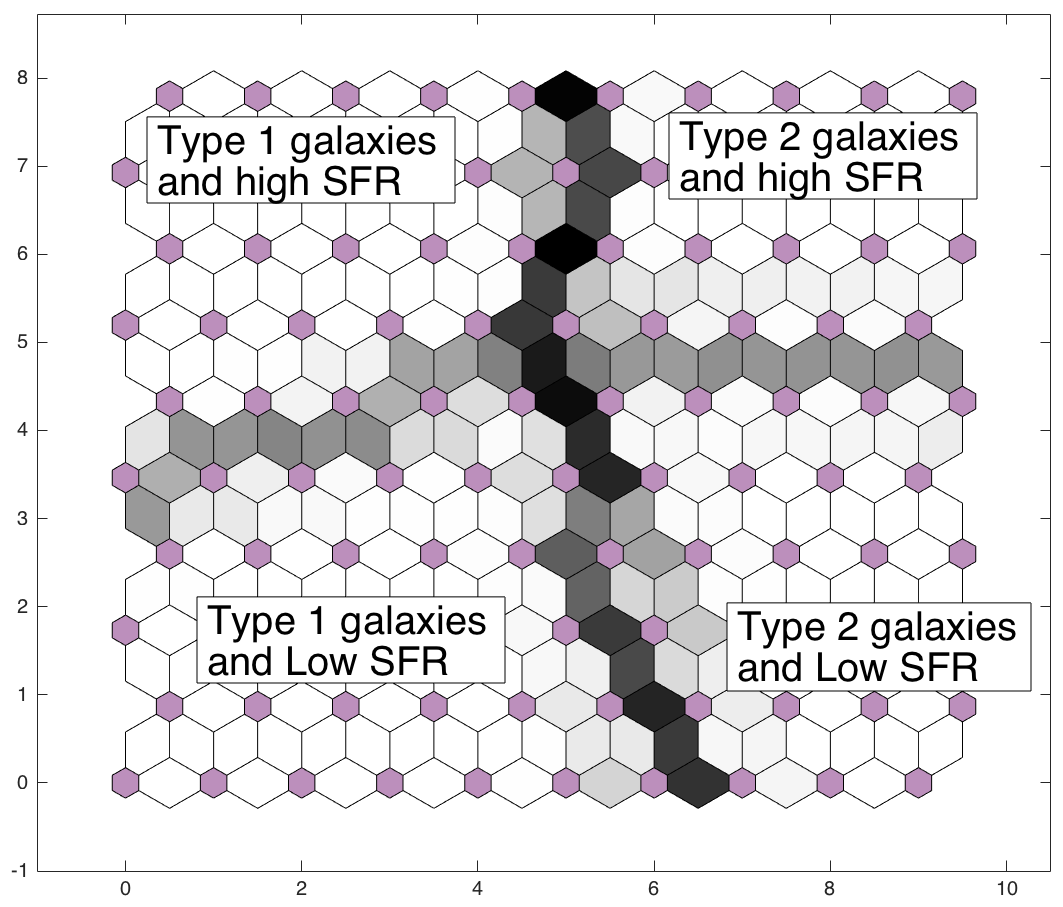
\includegraphics[width=\textwidth]{../image_paper2/sample/sample2_dist.png}
%             \end{subfigure}
%             \hfill
%             \begin{subfigure}[b]{0.5\textwidth}
%                 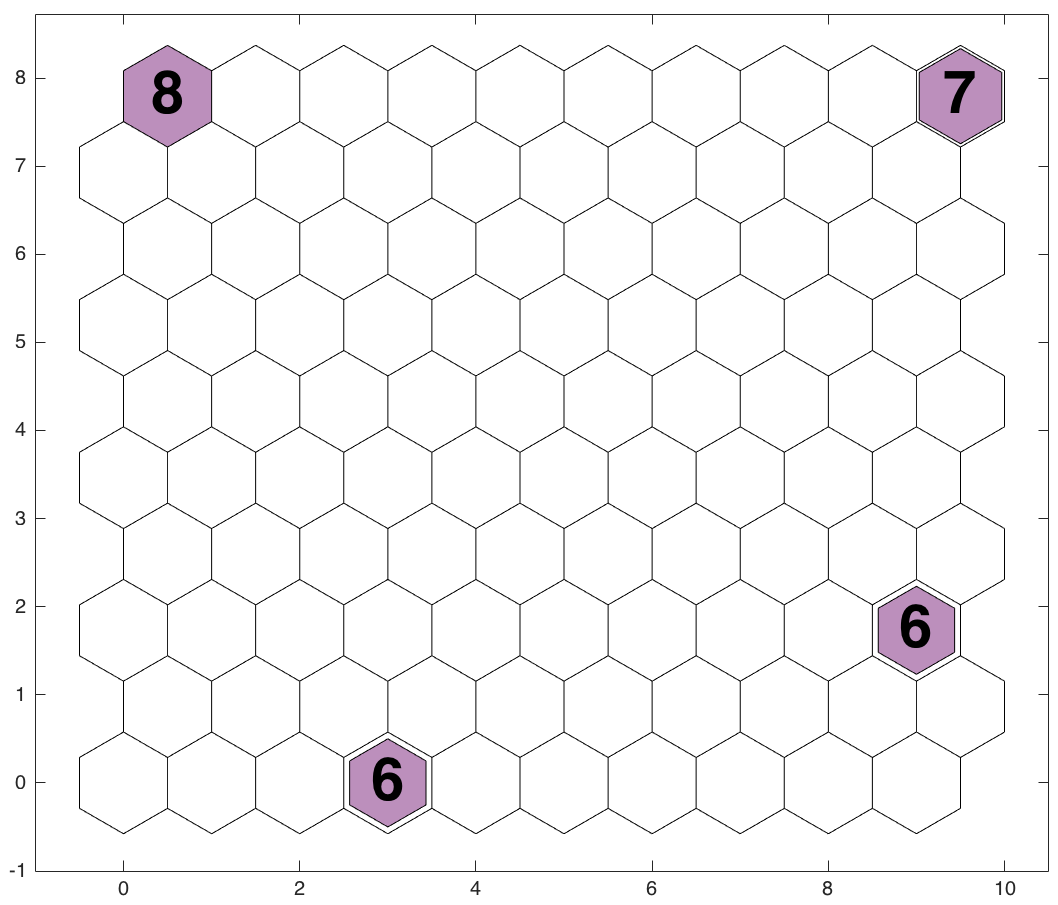
\includegraphics[width=\textwidth]{../image_paper2/sample/sample2_hits.png}
%             \end{subfigure}
%             \caption[Self-organizing map of the mock sample]{SOM of the mock sample. In both plots, the axes show the position of the neurons. Hexagonal shapes represent the neurons. The top plot is a distance map. The grey cycle colours show the differences between the weights of each neuron with white being the minimum difference and black being the maximum one. The lower plot is a ``hits plot". It represents the number of samples in each neuron, where empty means zero hits. In this sample, the 27 galaxies are clustered in 4 groups, containing 8, 7, 6 and 6 galaxies respectively.}
%             \label{fig: sample}
%         \end{figure}
 
%  To illustrate how self-organizing maps work, we create a mock sample of 27 galaxies.
%  The mock sample contains two attributes for each galaxy: the type (type 1 or type 2), and the star formation rate (high or low). 
%  We generated a SOM of size $10 \times 10$ using the same initial values mentioned in Section~\ref{sec: create_som}.

%  Fig. ~\ref{fig: sample} shows the SOM of this mock sample. 
%  The upper panel is the distance map. 
%  The axes show the position of the neurons in the $10 \times 10$ network.
%  The lower panel in Fig.~\ref{fig: sample} shows the hit map.
%  On this map, similar to the distance map, the axes show the position of the neurons and the hexagonal shapes are the neurons.
%  The number on the purple neurons shows the number of galaxies in that neuron.
%  Colour coverage of neurons depends on the number of the hits on the sample.
%  The neuron with the maximum number of hits is dark-coloured while the empty neurons are left uncoloured (white).
 
% Using this method, as expected, we are able to divide the mock sample galaxies into 4 distinct groups: Type 1 with high SFR, type 1 with low SFR, type 2 with high SFR and type 2 with low SFR. 
% The upper panel in the Fig.~\ref{fig: sample} clearly shows this division.
% In that plot, the upper half belongs to high star forming galaxies, while the lower half belongs to low star forming galaxies.
% The left half of the plot is where type 1 galaxies belong, and type 2 galaxies reside in the right side.
% Different shades of gray show the border between regions.
% The lower panel in Fig.~\ref{fig: sample} shows that only 4 neurons (out of 100) are occupied. 
% 8 galaxies are type 1 galaxies with high SFR, 7 are type 2 galaxies with high SFR, 6 are type 1 galaxies with low SFR and the other 6 are type 2 galaxies with low SFR. 
% We can conclude that although each galaxy had  the chance to occupy any of the neurons in the network, because of the similarity in the values of their attributes, they remained only in four groups.
% This network is considered a training network and can be used to cluster any new dataset with similar entries.


% As we show in the following sections, with data from real galaxies there are more than two dimensions and two galaxies never have exactly the same information. 
% If the network has enough neurons, the input data points would eventually separate from each other and cluster into smaller groups. 
% However, if the input data has high similarity, the number of neurons must be much higher than the number of input samples to be able to separate the groups from each other. 
% Therefore, it is up to the users to decide the similarity or dissimilarity between the input data based on number of neurons. 

%----------------------------------------------------------------------------------------
%----------------------------------------------------------------------------------------
%----------------------------------------------------------------------------------------
%Results
%----------------------------------------------------------------------------------------
%----------------------------------------------------------------------------------------
%----------------------------------------------------------------------------------------
%\include{sections_highz/}{results.tex}
%----------------------------------------------------------------------------------------
%----------------------------------------------------------------------------------------
%----------------------------------------------------------------------------------------
%Results
%----------------------------------------------------------------------------------------
%----------------------------------------------------------------------------------------
%----------------------------------------------------------------------------------------
\section{Results and Discussion}
\label{sec: result}

    In this section we show the results of the neural networks trained using the \citetalias{Kinney96} template spectra.
    Training with \citetalias{Kinney96} templates results in networks that have regions corresponding to galaxies of known morphological type. 
    The trained networks can then be used to categorize other galaxies.

    In order to find a sufficient size for the trained networks, we created maps with sizes ranging from $1\times2$ to $50\times50$.
    Varying the grid size of the maps helps us to monitor whether tighter grouping of galaxies is due to their similar properties or a lack of map space to separate them.
   Based on the size of the data and SOM results, we found the optimum grid size to be $1\times22$ and $12\times12$ in 1D and 2D maps, respectively. 
    For each grid we created different SOMs with different learning factors, neighbourhood distances, and number of iterations to find the optimum.
    We create the final SOMs with initial values for number of iterations in ordering phase, ordering phase learning factor, tuning phase learning factor, and tuning phase neighbourhood distance of 1000, 0.9, 0.02, and 1, respectively.
   
    We started our analysis by creating 1D SOMs. 
    First, we created SOMs with only two neurons ($1\times2$ map), and then increased the number of neurons one at a time in the 1D case (Section~\ref{sec: 1D_somz}).
    We generate 2D networks (Section~\ref{sec: 2D}),  again starting with the smallest possible number of neurons (4 neurons in a $2\times2$ map), increasing to 144 in a $12\times12$ map.    
    For each generated network, we compare the results with the \citetalias{Kinney96} categorization.
    We also use these networks to classify the \citetalias{Hossein12} galaxy sample, and compare this classification with that from the supervised networks in \citetalias{Hossein12}.

    \subsection{One-Dimensional Self-Organizing Maps}
    \label{sec: 1D_somz}
        \subsubsection{Training the Networks}
        \label{sec: 1Dt}
            To start our clustering, we assumed that galaxies can be divided into only two general types; quiescent and starburst.
            This corresponds to a network with only two neurons.
            We increased the size of the map gradually until the 12 input samples divide into the 12 neurons. 
        
            Figs.~\ref{fig: 1by2T} --\ref{fig: 1by22T} show the results of the training networks.
            As in Fig.~\ref{fig: sample}, the upper part of the figures shows the neurons and their relative distances between weight of neurons.
            As mentioned in Section~\ref{sec: method_somz}, an increase in the darkness of colours between neurons represents an increase in relative distance between the neurons.
            The lower panels of the figures show the number of \citetalias{Kinney96} templates that are placed in each neuron. 
            \begin{figure}
                \begin{subfigure}[b]{\textwidth}
                    \centering
                  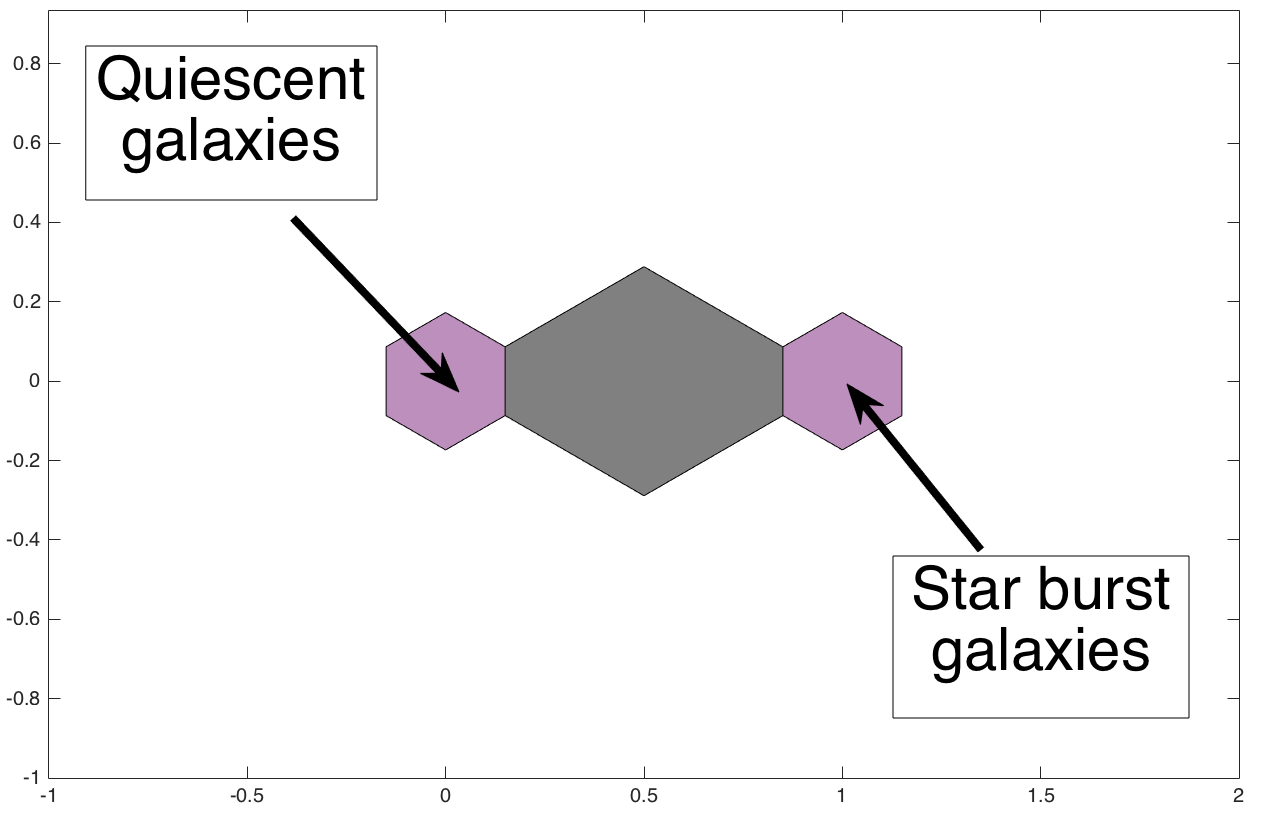
\includegraphics[width=0.8\textwidth]{../image_paper2/1d/dist_1_by_2.png}
                \end{subfigure}
                \hfill
                \begin{subfigure}[b]{\textwidth}
                    \centering 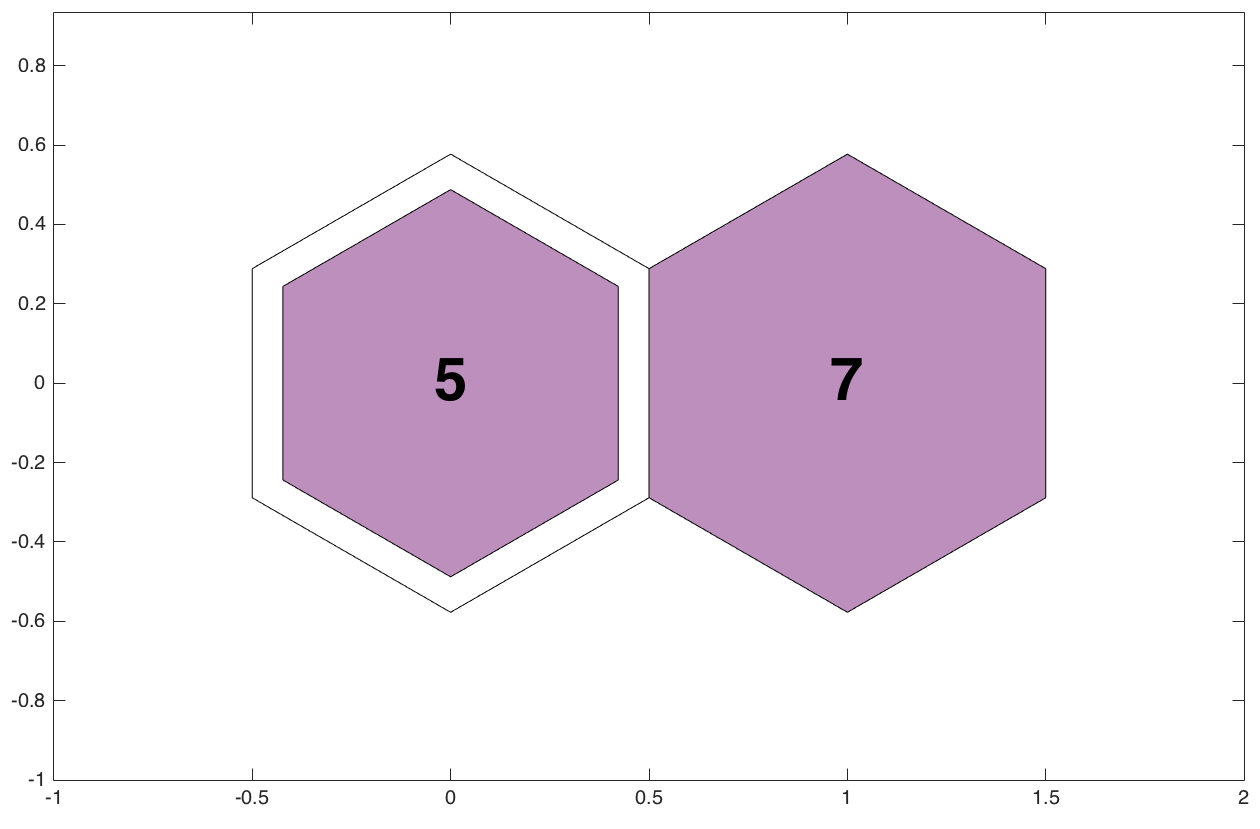
\includegraphics[width=0.8\textwidth]{../image_paper2/1d/hit_t_1_by_2.png}
                \end{subfigure}
                \caption[Results of training network in $1\times2$~grid]{Results of training network in $1\times2$~grid. As in Fig.~\ref{fig: sample}, the upper panel is a distance map and the lower panel is a hit map. In this network, 5 of the templates from \citet{Kinney96} are categorized as quiescent galaxies and the rest are starbursts. Because of their strong emission lines, Sc galaxies are moved towards the starburst ones.}
                 \label{fig: 1by2T}
            \end{figure}
        
        
            In the upper map in Fig.~\ref{fig: 1by2T}, the dark colour between two neurons indicates that the relative distance between these two groups are relatively high, and these two groups are distinguishable groups.
            In the lower part of Fig.~\ref{fig: 1by2T}, we see that the templates are divided into two groups of 5 and 7.
            Although we know from \citetalias{Kinney96} and \citetalias{Hossein12} that 6 of the templates are quiescent and the other 6 are starbursts, the SOM results show 5 of the galaxies in one group and the other 7 in the second group.
            In this method, the Sc template has been categorized as starburst due to the relatively higher disk stellar population relative to that of the bulge. 
            According to \citetalias{Kinney96}, Sc galaxies are considered to be late Hubble type galaxies which have  flattter spectra compare to other quiescent galaxies. 
            

            Fig.~\ref{fig: 1by3T} shows the results of the training in a 1$\times$3 network.
            In these plots we force the galaxies to be categorized in a maximum 3 groups. 
            If the templates in Fig.~\ref{fig: 1by2T} truly belonged in two groups, they would be grouped into two groups in this network, even when we try to cluster them into three. 
            However, in the lower panel of Fig.~\ref{fig: 1by3T}, we can see that the middle node contains two templates.
            These two templates, which are separated from the group of starburst templates in the lower part of Fig.~\ref{fig: 1by2T},  are the SB5 and SB6 types.
            In the upper plot of Fig.~\ref{fig: 1by3T}, the colour between two right neurons is black and the colour between two left neurons is white. 
            The black colour indicates that the left neuron is completely different from the other two groups,
            while the white colour shows that the two right neurons are very similar to one another. 
            
            Comparing Fig.~\ref{fig: 1by2T} to Fig.~\ref{fig: 1by3T} shows that the starburst templates are divided into two groups. 
            Based on the colours between these two groups, we conclude that they are very similar; both groups are starbursting and have strong emission lines.
            On the other hand, the SB5 and SB6 templates have the highest internal extinctions; this causes the spectra to become flatter at shorter wavelengths. 
            The flatter UV spectra make these two templates more similar to quiescent galaxies than to other starbursts.
            Therefore, in the networks, SB5 and SB6 types are grouped close to the quiescent galaxy templates.
                
            \begin{figure}
                \begin{subfigure}[b]{\textwidth}
                    \centering
                    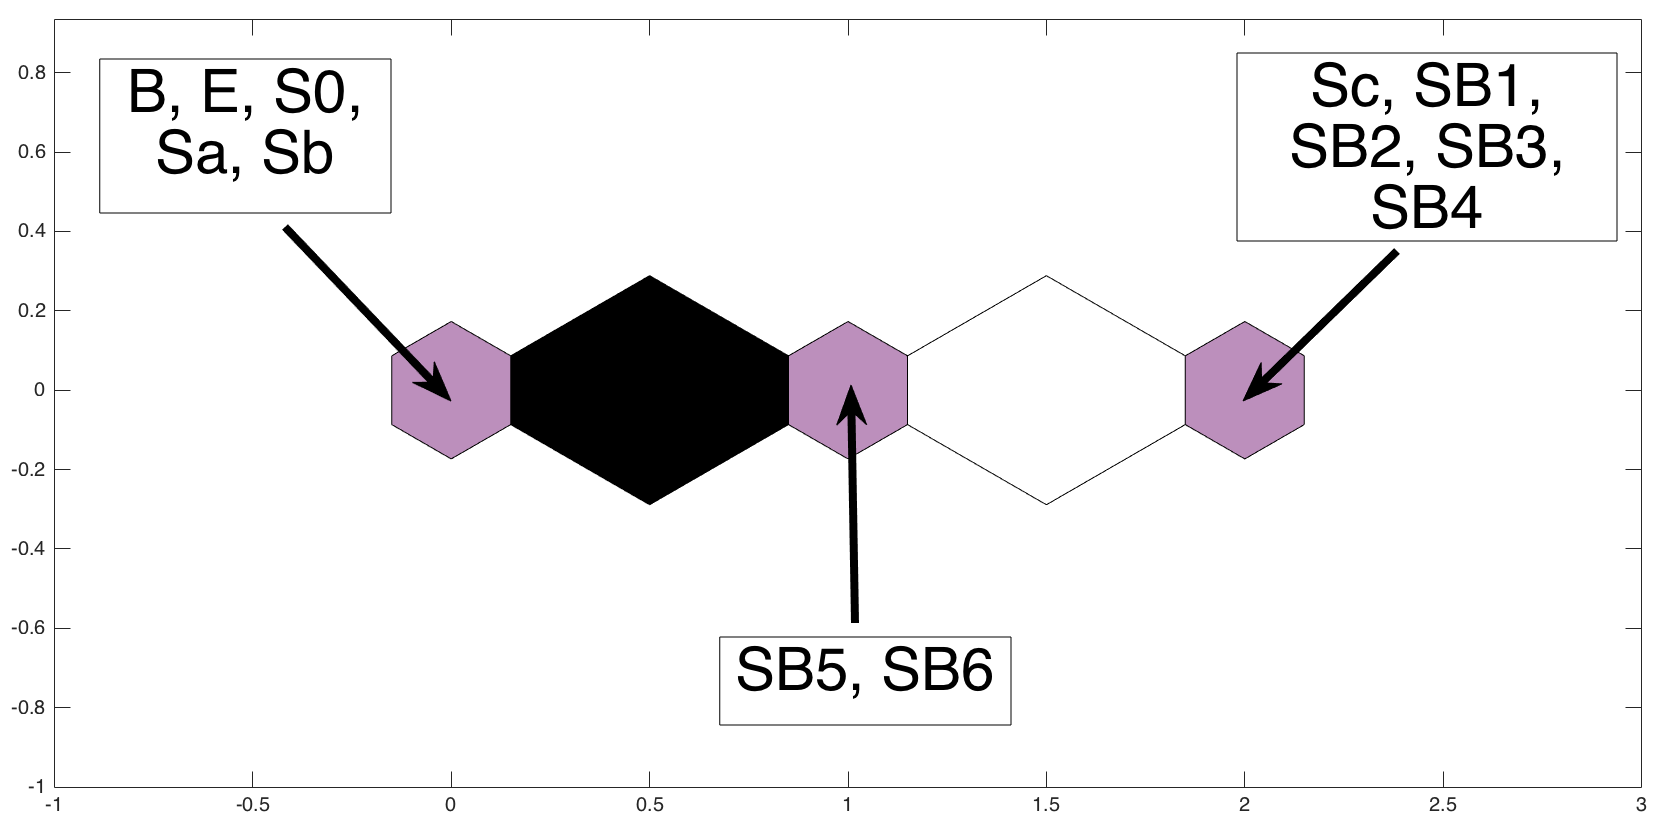
\includegraphics[width=\textwidth]{../image_paper2/1d/dist_1_by_3.png}
                \end{subfigure}
                \hfill
                \begin{subfigure}[b]{\textwidth}
                     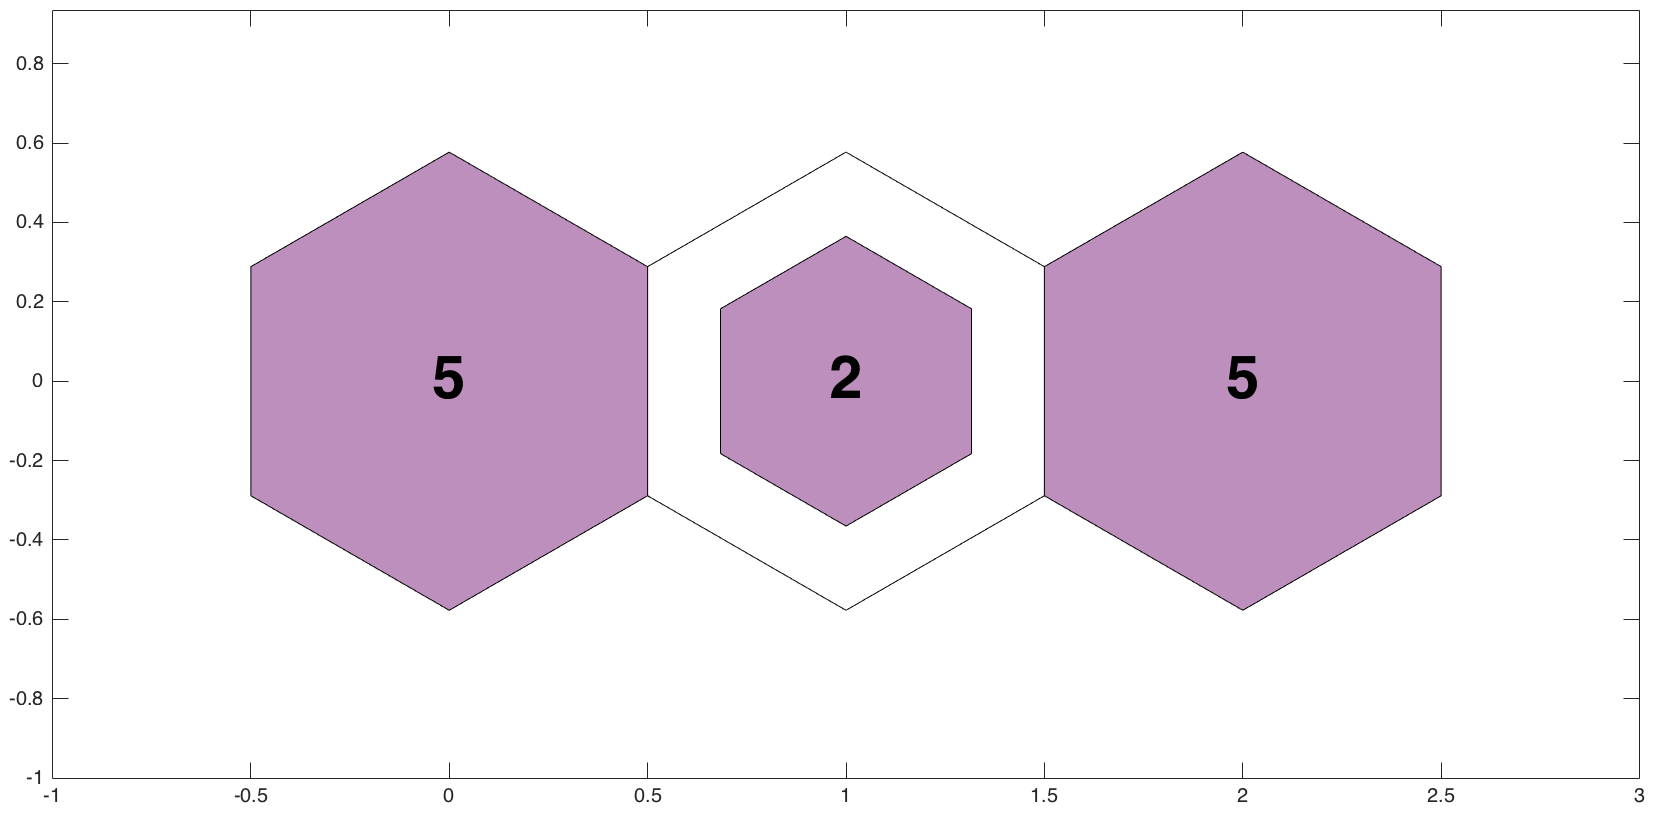
\includegraphics[width=\textwidth]{../image_paper2/1d/hit_t_1_by_3.png}
                \end{subfigure}
                \caption[Results of training network in $1\times3$~grid]{The same as Fig.~\ref{fig: 1by2T} but showing the results of training network in $1\times3$~grid. In this network again, 5 of the \citet{Kinney96} templates are categorized as quiescent and 7 as starbursts. However, this time 2 templates (SB5 and SB6) are separated from the starburst groups.}
                 \label{fig: 1by3T}
            \end{figure}
           
            We increased the size of the maps gradually until the galaxies are divided into twelve groups (Figs.~\ref{fig: 1by4T} to ~\ref{fig: 1by20T} in Appendix~\ref{app: high_Z_1d_soms} and ~\ref{fig: 1by22T}).
            Since there are more nodes in higher grid SOMs, the algorithm 
            pays more attention to small differences between groups.
            If the templates from \citetalias{Kinney96} had completely distinct spectral types, then a $1\times12$-sized SOM would be expected to show 12 different groups each containing a single template.
            However, in Fig.~\ref{fig: 1by12T}, we see that three of the neurons contain two templates and three of them are empty.
            It is evident that there was no template in the \citetalias{Kinney96} sample that can fill those empty neurons.
            In Fig.~\ref{fig: 1by12T}, from left to right, templates with types B and E, SB3 and SB4, and SB1 and SB2 are the ones grouped together. 
            The SB3 and SB4 grouping breaks when we increase the size of the network to $1\times15$~(Fig.~\ref{fig: 1by15T}).
            The SB1 and SB2 templates, however, remain in the same neuron until the size of the map is increased to $1\times20$~(Fig.~\ref{fig: 1by20T}).
            The separation between templates B and E only happens when the size of the SOM exceeds $1\times22$~(Fig.~\ref{fig: 1by22T}).
        \begin{figure}
            \begin{subfigure}[b]{\textwidth}
                \centering
                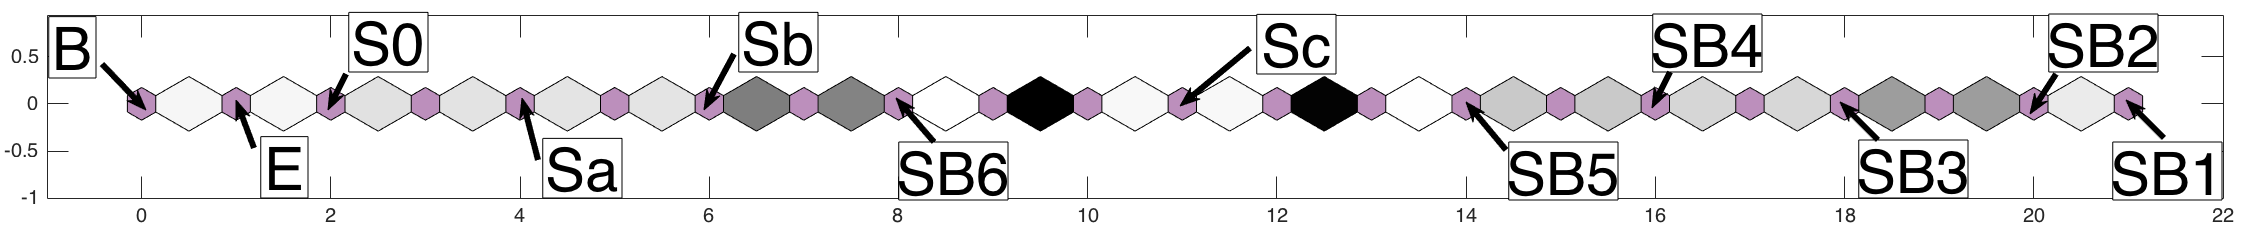
\includegraphics[width=\textwidth]{../image_paper2/1d/dist_1_by_22.png}
            \end{subfigure}
            \hfill
            \begin{subfigure}[b]{\textwidth}
                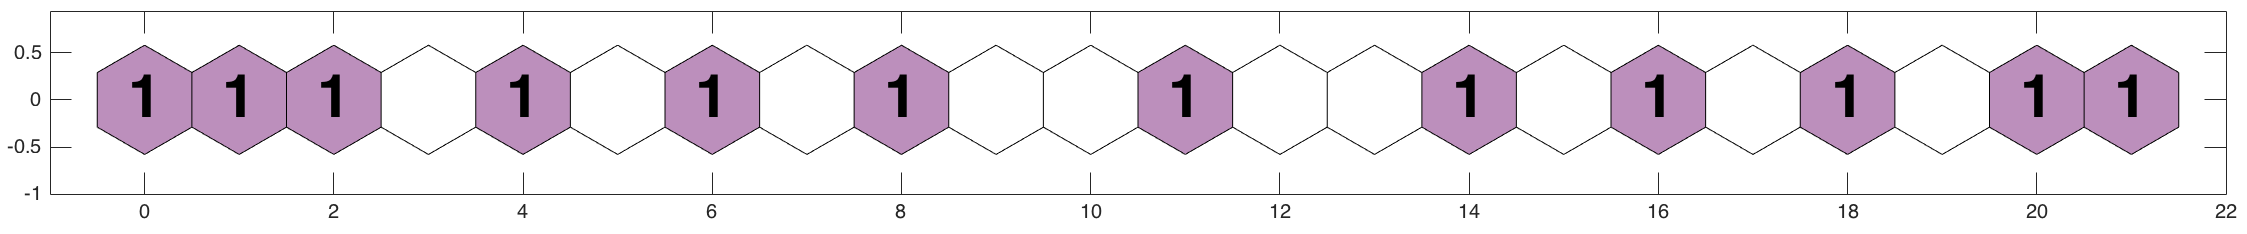
\includegraphics[width=\textwidth]{../image_paper2/1d/hit_t_1_by_22.png}
            \end{subfigure}
            \caption[Results of training network in $1\times22$~grid]{The same as Fig.~\ref{fig: 1by2T} but this time the figure shows results of training network in $1\times22$~grid.}
            \label{fig: 1by22T}
        \end{figure} 
    
            In Fig.~\ref{fig: 1by22T}, we can see twelve different groups:
            5 groups in the left-side neurons are separated from 7 groups on the right side of the map with two dark-grey colours between them.
            This shows that even though the galaxies are clustered in twelve groups, there still remain only two main distinct groups.
            The closest occupied neuron in the starburst side of the SOM, belongs to the SB6 type. 
            This template has the most extinction and its spectrum has more similarity to quiescent galaxies than other starburst types. 
            
            The fact that the templates need to have at least 22 different neurons to be divided into 12 groups shows that the differences between SB1 and SB2, and B and E, templates are very small.
            Because of their similarities, they tend to stay in the same group until the network becomes big enough to make attention to the smallest particularity.
           
        \subsubsection{Classifying the Galaxy Sample}
         \label{sec: 1Dv}
            After training the networks as discussed in Section~\ref{sec: 1Dt}, we used them to classify the fitted SEDs of the sample of 142 galaxies from \citetalias{Hossein12}.
            The upper panel in Fig.~\ref{fig: 1by2V} shows the result of this classification using the $1\times2$~network from Fig.~\ref{fig: 1by2T}.
            Eighty of the galaxies have spectral types similar to those of the quiescent galaxies and the spectral types of the rest are similar to the starburst galaxies.
            The lower left panel shows the median spectrum of the 80 galaxies that were classified as quiescent. 
            These galaxies are similar to the ones in the left node in the upper panel of Fig.~\ref{fig: 1by2T}:
            the spectra clearly show the 4000\AA~break, one of the signatures of quiescent galaxies.
            The H$\alpha$ emission in the spectrum could be from galaxies with similar spectral types to Sa galaxies, but with stronger emission lines.
            The median spectrum in the lower right panel of Fig.~\ref{fig: 1by2V} shows strong emission lines and bright ultraviolet continuum, indications of a high star formation rate.
            \begin{figure}
                \begin{subfigure}[b]{\textwidth}
                    \centering
                    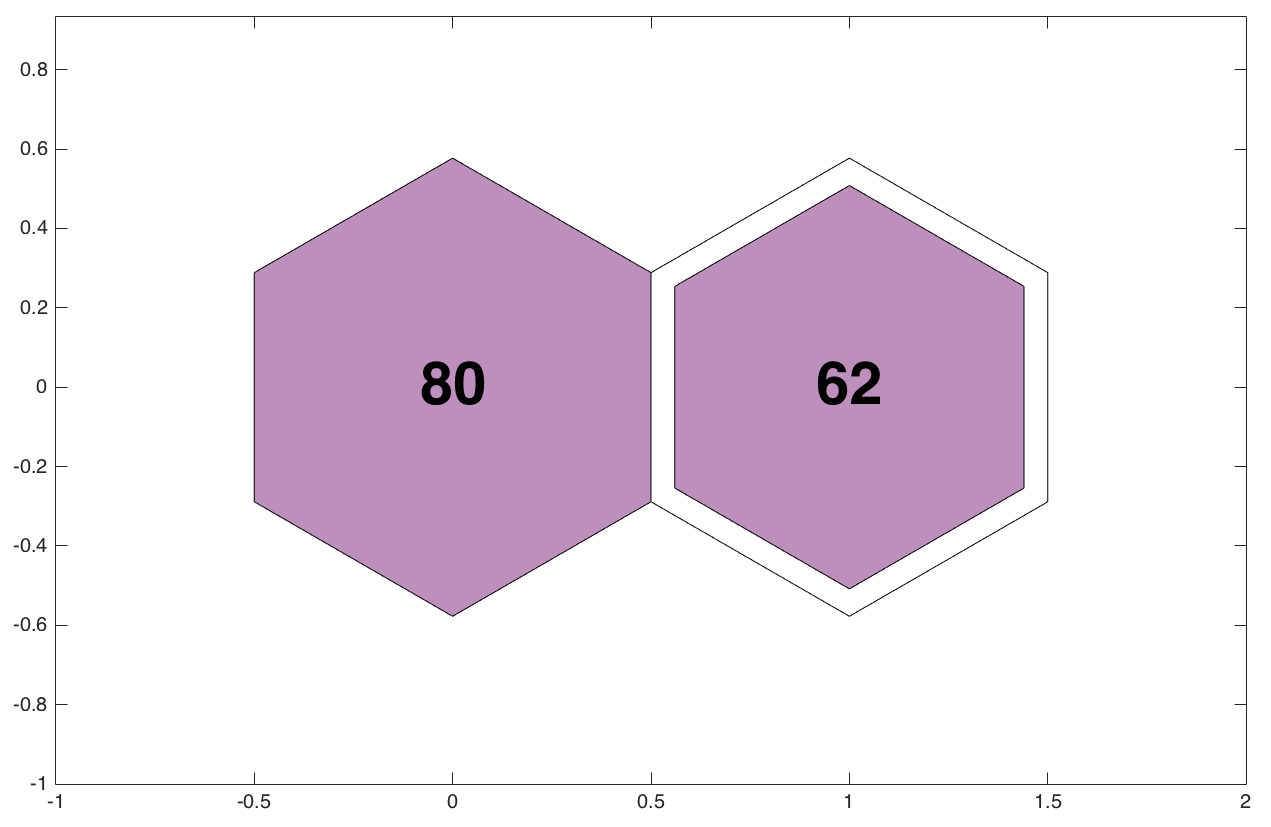
\includegraphics[width=\textwidth]{../image_paper2/1d/hit_v_1_by_2.png}
                    %\caption{$1\times2$ weight map}
                     %\label{fig: 1by3T}
                \end{subfigure}
                \hfill
                \begin{subfigure}[b]{\textwidth}
                     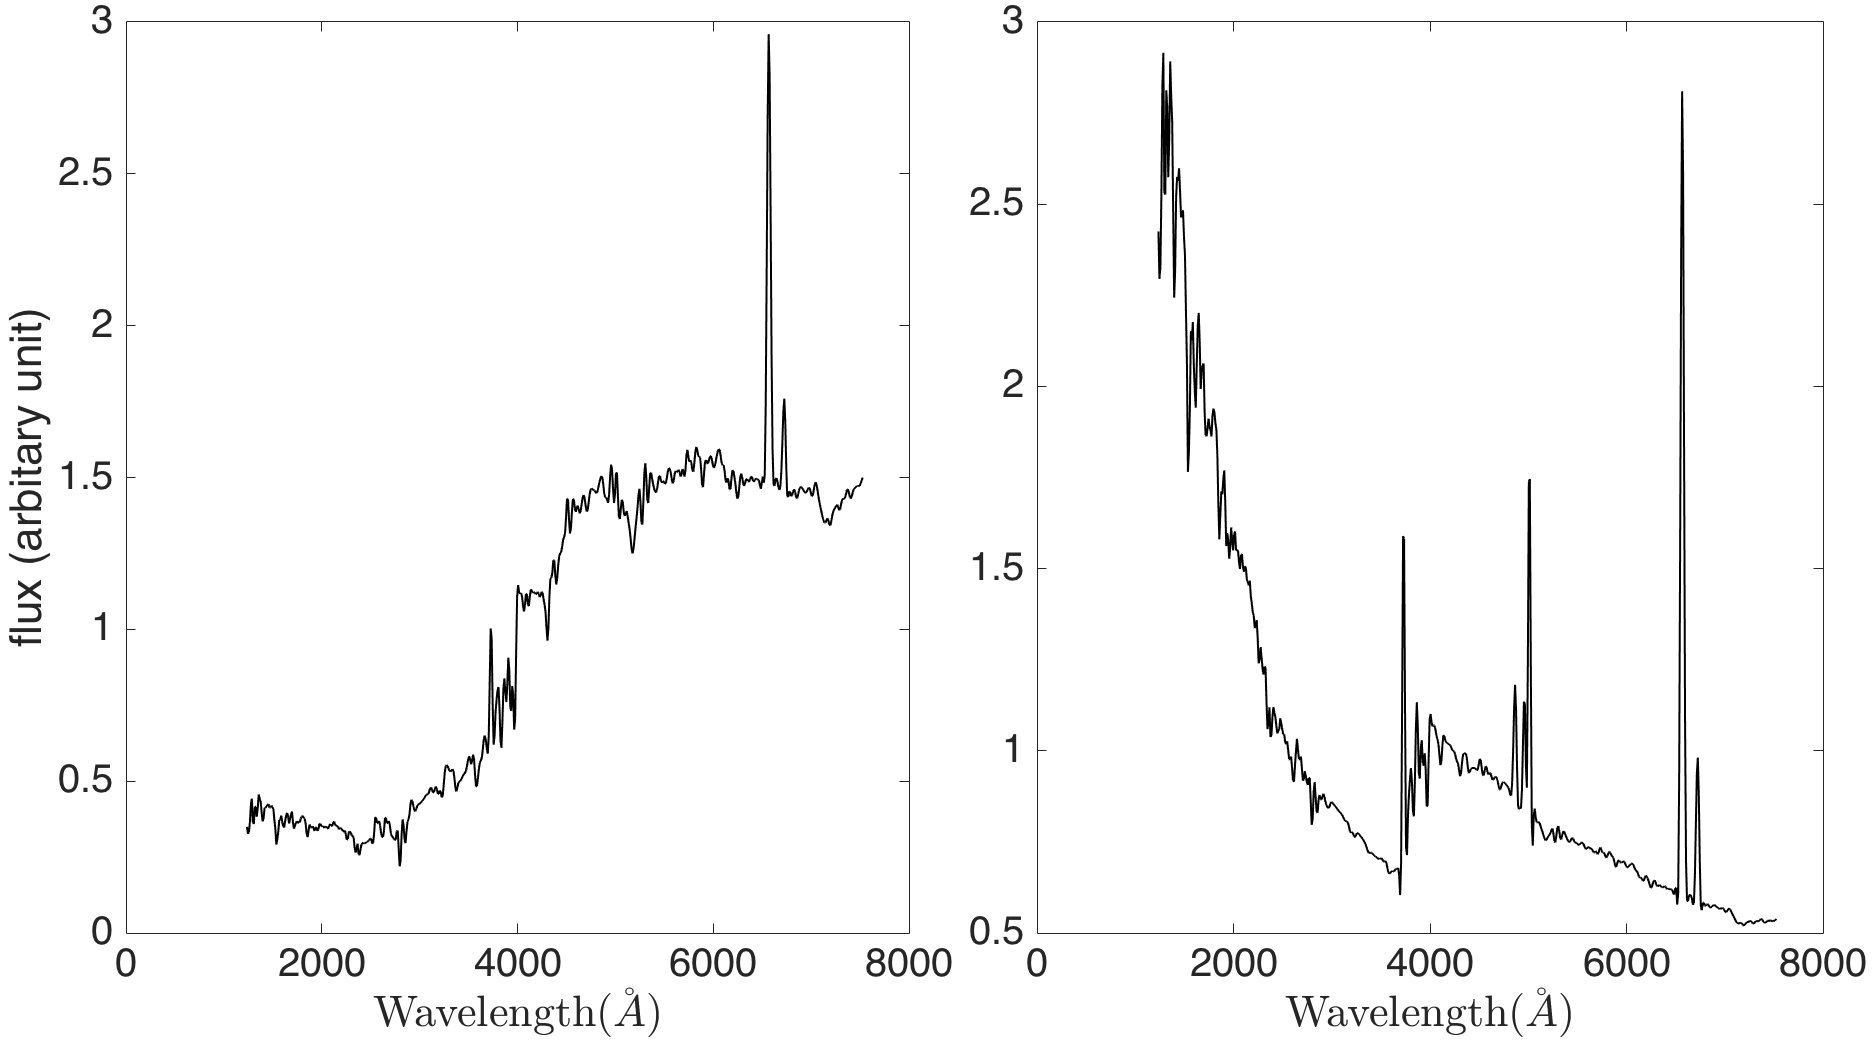
\includegraphics[width=\textwidth]{../image_paper2/1d/SED_total1by2.png}
                     %\caption{$1\times2$ hits map}
                     %\label{fig: 1by3Thits}
                \end{subfigure}
                \caption[Classification of fitted galaxy SEDs from \citet{Hossein12} using the $1\times2$~networks]{Classification of fitted galaxy SEDs from \citet{Hossein12} using the $1\times2$~network trained from the \citet{Kinney96} templates (Fig.~\ref{fig: 1by2T}). Upper panel: a hit map with the number in each node representing the number of galaxies belonging to that group. In this case 80 means that 80 of the 142 spectra are classified into the quiescent group while the 62 of the 142 spectra are categorized as starburst galaxies. Lower panel: median spectra of the galaxies in each group (fluxes are normalized by dividing spectra by flux at 4000\AA), early-type on the left and starburst on the right.}
                \label{fig: 1by2V}
            \end{figure}          
            
            Since in this network galaxies were forced to be divided into a maximum of two groups, the strongest feature in a galaxy's spectrum predominantly decides which group the galaxy belongs to.
            Galaxies with a weak 4000\AA~break but strong emission lines and ultraviolet upturn are categorized as starbursts while galaxies with a strong 4000\AA~break are categorized as quiescent.
            Increasing the size of the SOM helps solve the problem of the galaxies which have features that are common in both groups.
            
            Fig.~\ref{fig: 1by3V} presents the result of classifying the spectra of the galaxies using the $1\times3$~network (from Fig.~\ref{fig: 1by2T}): 66 of the galaxies belong to the quiescent group, and 47 belong to the starburst group. 
            However, 29 of the galaxies are similar to starbursts in some, but not all, of their features. 
            Galaxies in this group have strong emission lines and are ultraviolet-bright, but they also have a strong 4000\AA~break, which makes them cluster closer to the quiescent galaxies (middle panel in the lower part of Fig.~\ref{fig: 1by2V}).

            \begin{figure}
                \begin{subfigure}[b]{\textwidth}
                    \centering
                    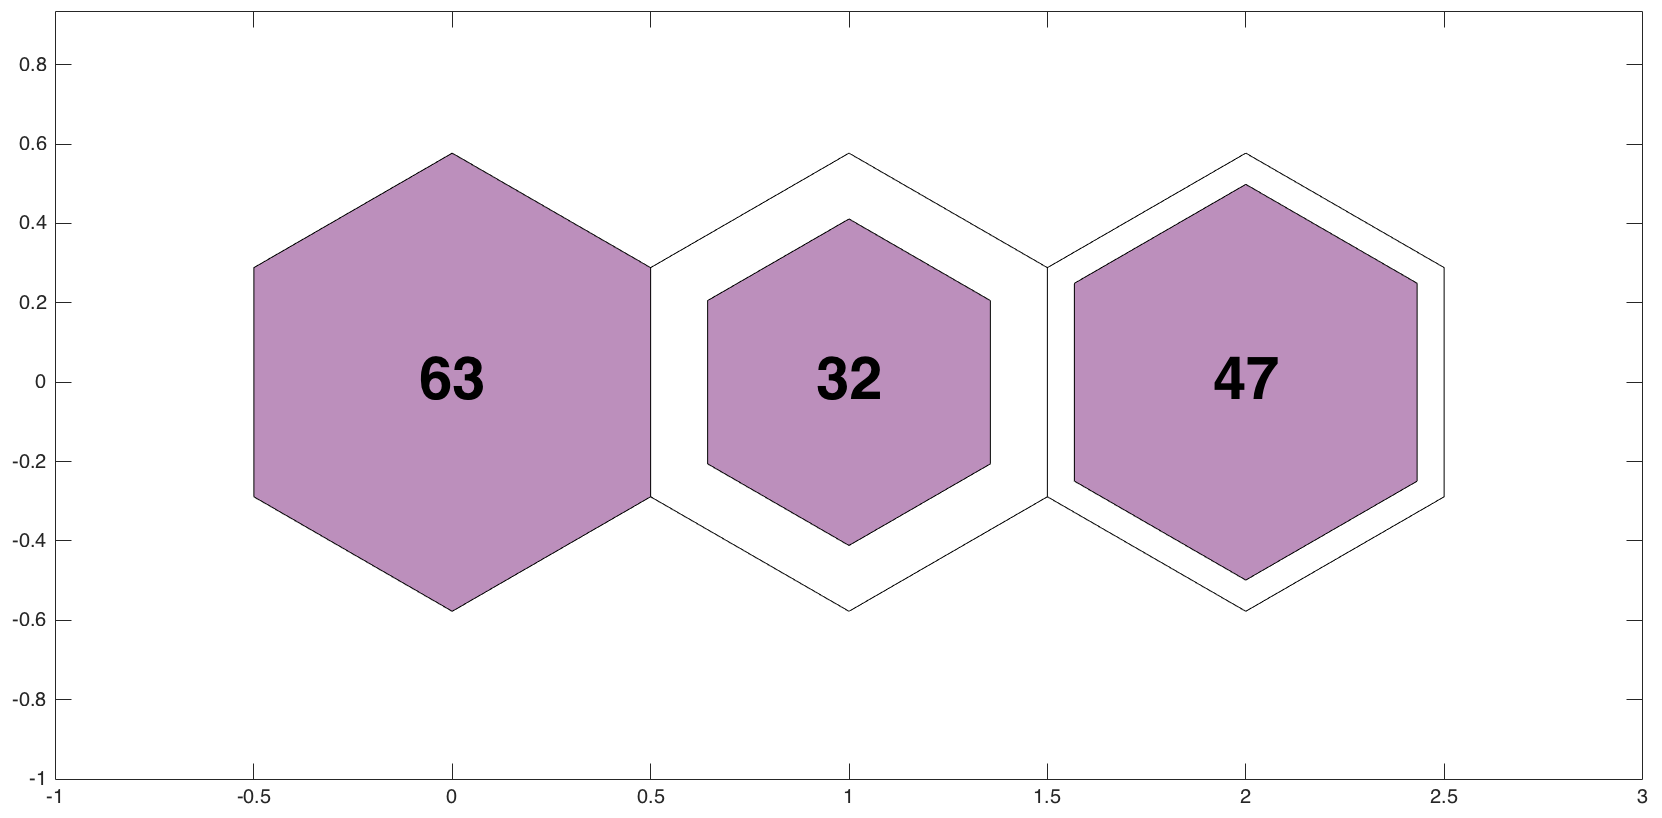
\includegraphics[width=\textwidth]{../image_paper2/1d/hit_v_1_by_3.png}
                \end{subfigure}
                \hfill
                \begin{subfigure}[b]{\textwidth}
                     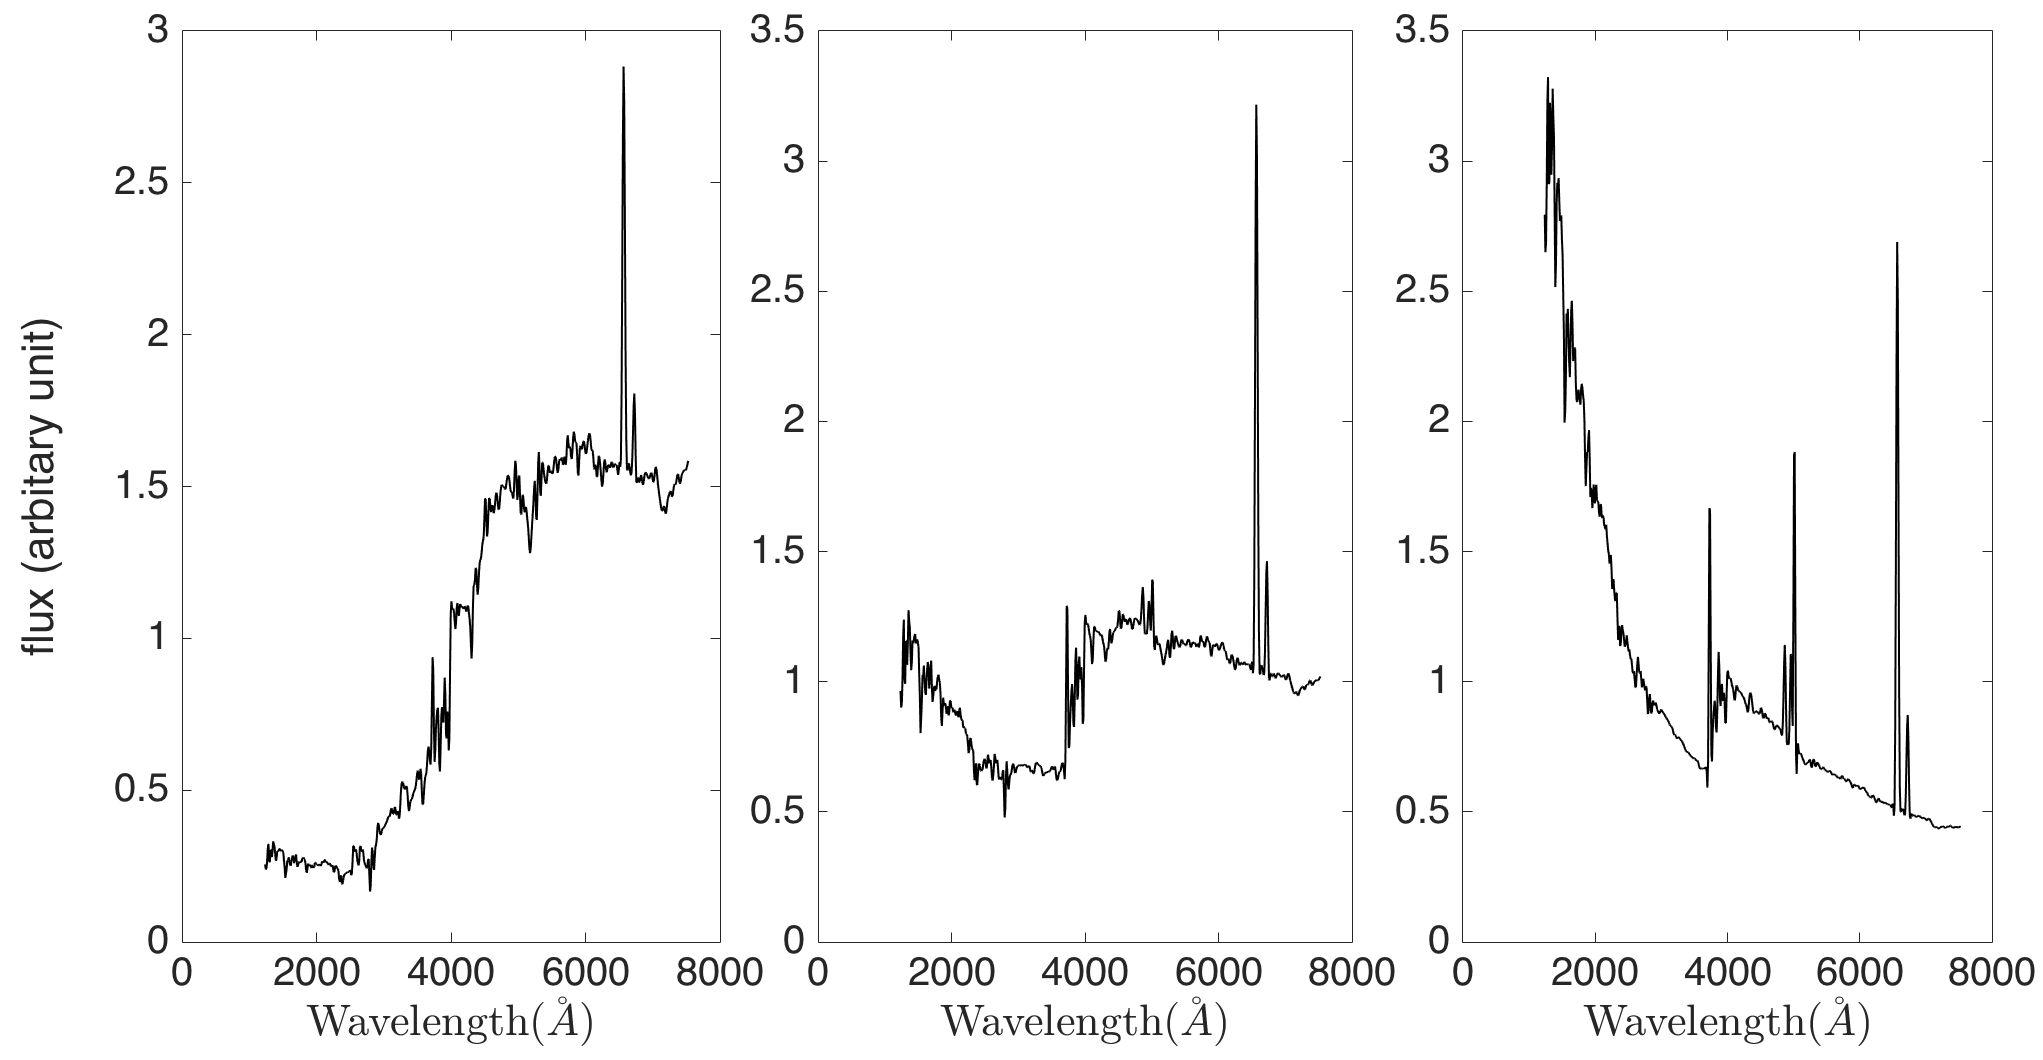
\includegraphics[width=\textwidth]{../image_paper2/1d/SED_total1by3.png}
                \end{subfigure}
                \caption[Classification of fitted galaxy SEDs from \citet{Hossein12} using the $1\times3$~networks]{Same as Fig.~\ref{fig: 1by2V}, but in this figure, we used a network with size of $1\times3$ (Fig.~\ref{fig: 1by3T}) to classify the sample galaxies.}
                \label{fig: 1by3V}
            \end{figure}       
            
            In Fig.~\ref{fig: 1by22V}, we use the $1\times22$~network to classify the sample galaxies.
            As mentioned in Section~\ref{sec: 1Dt}, in this network size we observed the first separation of the \citetalias{Kinney96} galaxies into 12 different neurons.
           As in Figs.~\ref{fig: 1by2V} and ~\ref{fig: 1by3V}, the upper panel of Fig.~\ref{fig: 1by22V} shows the number of galaxies (out of the 142) belonging to each neuron in the $1\times22$ SOM.

            \begin{figure}
                \begin{subfigure}[b]{\textwidth}
                    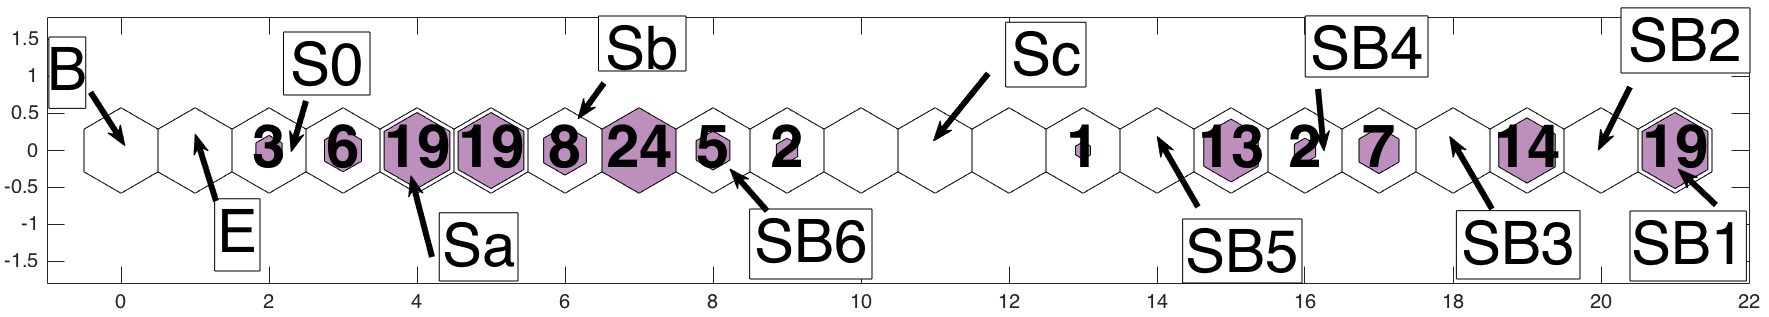
\includegraphics[width=\textwidth]{../image_paper2/1d/hit_v_1_by_22_n.png}
                    \centering
                \end{subfigure}
                \hfill
                \begin{subfigure}[b]{\textwidth}
                \centering
                     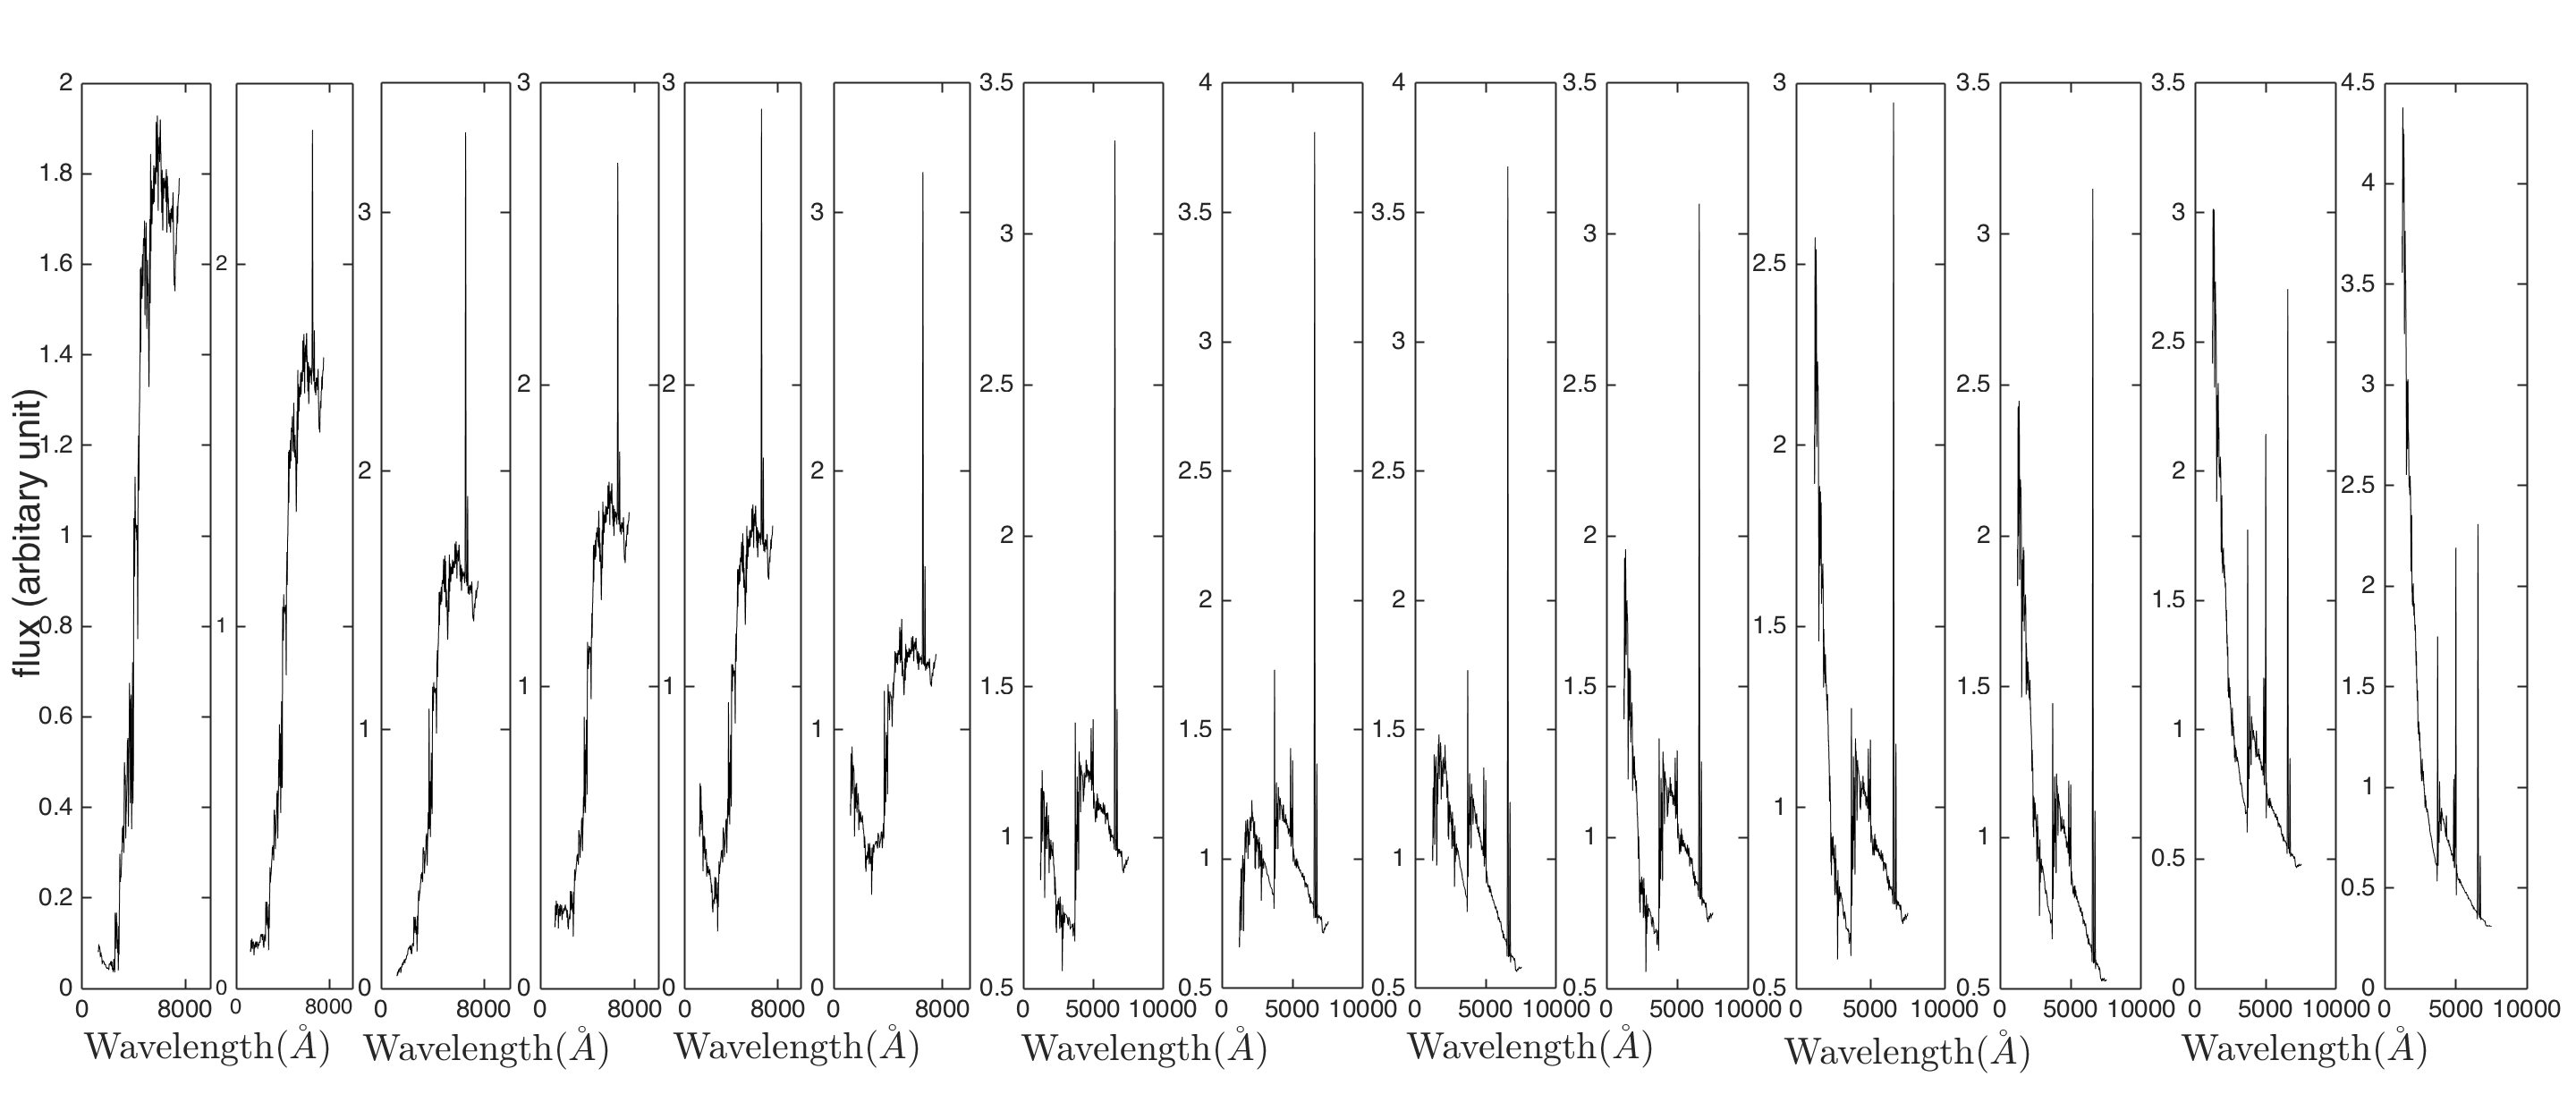
\includegraphics[width=\textwidth]{../image_paper2/1d/SED_total1by22.png}
                \end{subfigure}
                \caption[Classification of fitted galaxy SEDs from \citet{Hossein12} using the $1\times22$~networks]{Same as Fig.~\ref{fig: 1by2V}, but in this figure, we used a network with size of $1\times22$ (Fig.~\ref{fig: 1by22T}) to classify the sample galaxies. In the median spectra of each neuron, we can clearly see the changes from quiescent galaxies to the starburst ones. The 4000\AA~ break weakens from left to right and the emission line strengths increase.}
                \label{fig: 1by22V}
            \end{figure}

            The lower panels present the median spectra of the galaxies in each neuron.
            Since galaxies had more space to separate, some of the neurons are left empty.
            Thus, instead of having 22 median spectral plots in the lower part of Fig.~\ref{fig: 1by22V}, there are only 12.
            
            Comparing the upper panel of Fig.~\ref{fig: 1by22V} with the lower panel of Fig.~\ref{fig: 1by22T} shows that the occupied neurons are not necessarily the same.
            If a cluster from the \citetalias{Hossein12} sample fills the same neuron as a \citetalias{Kinney96} template, we can conclude that the spectra of galaxies in the cluster are very similar to those of the template.
            Otherwise, we can conclude that the spectra of galaxies in the cluster are (dis)similar to two of the \citetalias{Kinney96} templates.
            For the latter case, the colours establish which template has greater similarity to the \citetalias{Hossein12} cluster.
            
            The first two neurons in the upper plot in Fig.~\ref{fig: 1by22V} are empty, while these neurons were occupied by galaxies B and E in the trained network.
            We therefore conclude that there are no galaxies in the \citetalias{Hossein12} sample with spectral type similar to that of type B or E.
            There are 3 galaxies in the third neuron, similar to the S0 type. 
            19 of the galaxies are in the fifth neuron and similar to the Sa type, while the 6 galaxies in the fourth neuron have spectral type similar to both S0 and Sa galaxies.
            There are 8 Sb type galaxies and 19 galaxies with spectral types similar to both Sa and Sb type galaxies.
            The following two neurons (eighth and ninth neurons from the left) are on the edge of the quiescent and starburst galaxies.
            In the upper panel in Fig.~\ref{fig: 1by22T}, the colour between these two neurons is black, which shows that these two are very different.
            Therefore, 24 galaxies in the eighth neuron have similar spectra to Sb type galaxies, and the spectra of the 5 galaxies in the ninth neuron are similar to the SB6 galaxies.
            The far right neurons in the network belong to galaxies with spectra comparable to types SB1 and SB2.
            
            In general, 56 galaxies correspond exactly to \citetalias{Kinney96} templates and the other 86 are placed between the initial 12 suggestions.
            As \citetalias{Hossein12} mentioned, part of the reason we could not classify all the galaxies using the \citetalias{Kinney96} model is that the model was constructed from co-adding spectra of 70 galaxies.
            In this small sample, it is quite possible that the best SEDs do not match any model perfectly and the original classifications have high uncertainties.
            
            With other methods (e.g. $\chi^2$ fitting), trained neural network fitting of spectra is limited to models and the results are always reported with uncertainties.
            However, with SOM, we have the freedom to categorize galaxies in intermediate groups.
            Therefore, if the spectra of galaxies do not match completely with any of the spectral templates in Fig.~\ref{fig: k96}, they can be categorized as a spectrum with similarity to two or more of the groups.

                        
        
        
        \subsubsection{Properties of the Clustered Galaxies}
        
        In order to check whether our conclusions in Section~\ref{sec: 1Dv}~are correct, in this section we test the relations between median properties of the galaxies in each neuron.
        
        \begin{figure}
            \centering
            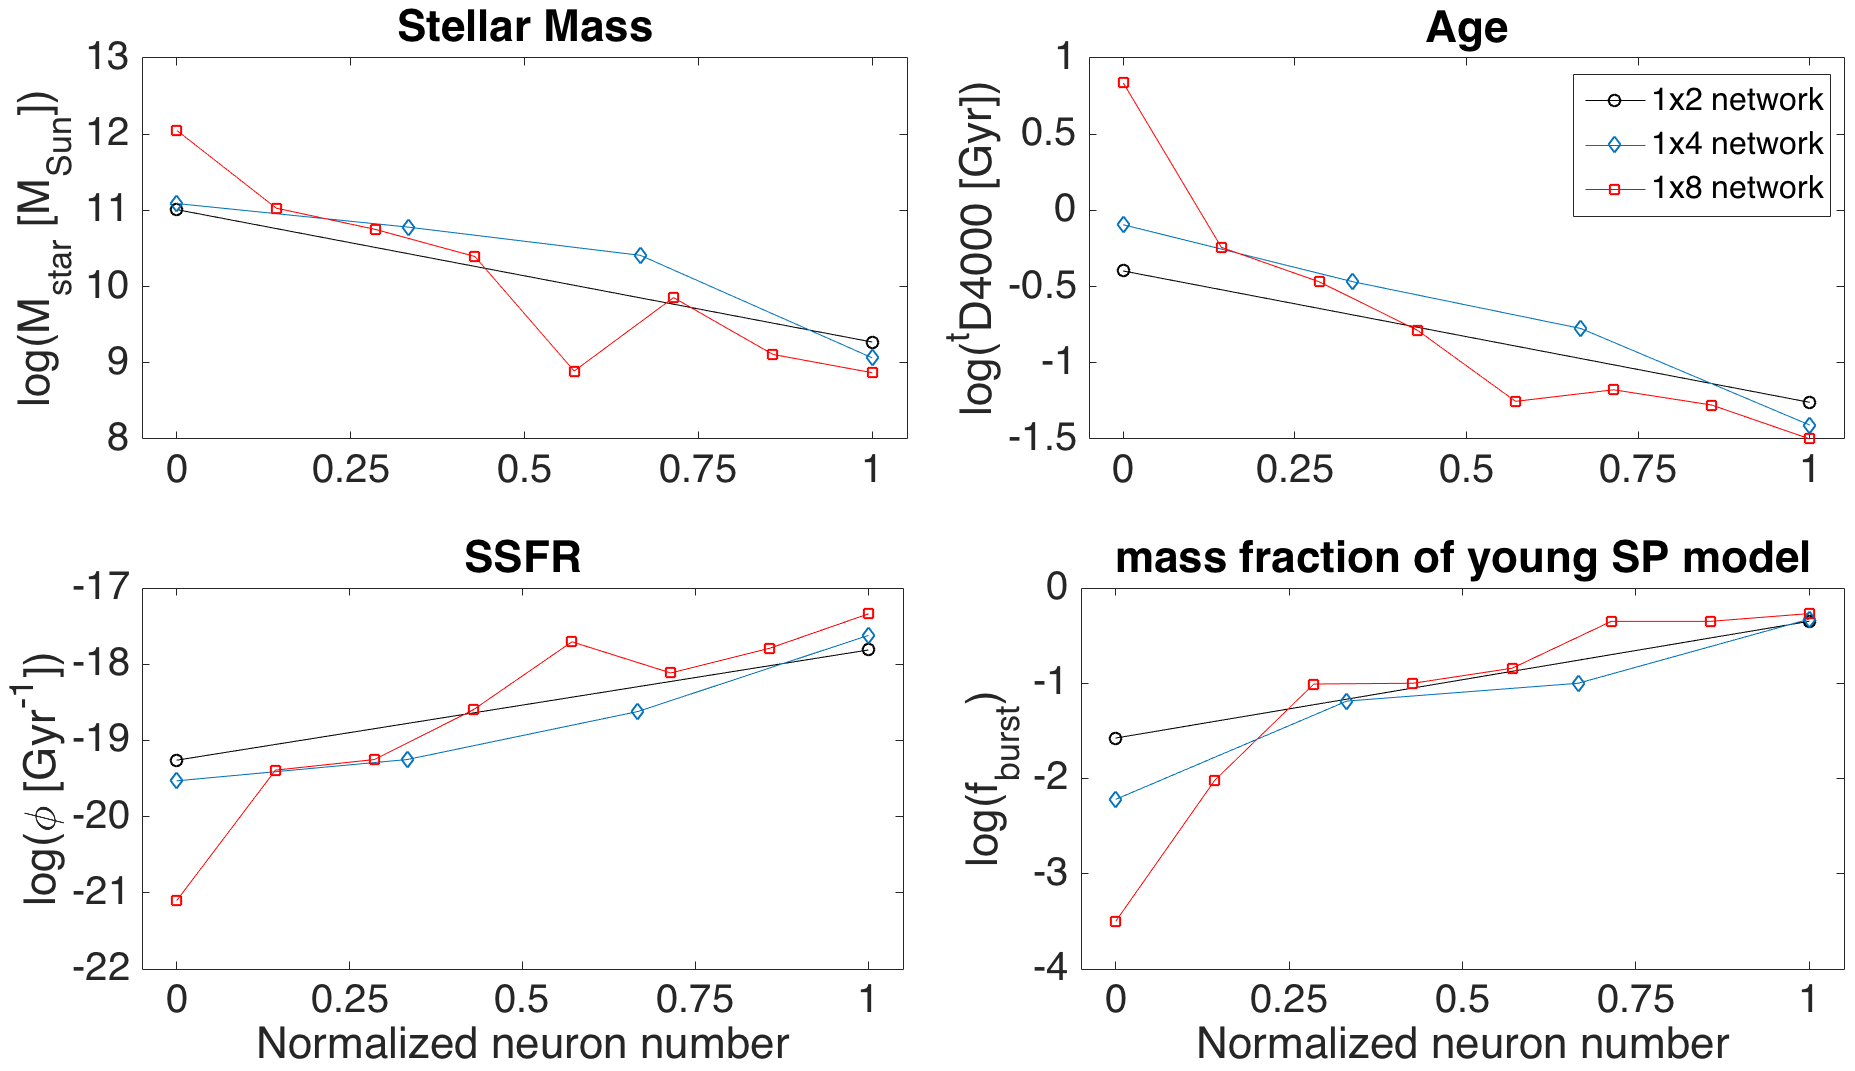
\includegraphics[width=\textwidth]{../image_paper2/1d/props5.png}
            \caption[The median of four properties of galaxies in three networks]{Comparing the median of four properties of galaxies in each node in $1\times2$ (black circles), $1\times4$ (blue diamonds), and $1\times8$ (red triangles) networks.}
            \label{fig: props}
        \end{figure}
       
        Fig.~\ref{fig: props} shows the median of stellar mass, age, specific star formation rate (sSFR; star formation rate per stellar mass), and $f_\mathrm{burst}$ of the galaxies in each neuron in the $1\times2$, $1\times4$, and $1\times8$ networks.
        In all plots, the horizontal axis is the number of the neurons divided by the size of the network.%, and vertical axis is one of the aforementioned properties.
%        
        As shown in Fig.~\ref{fig: props}, in all three networks, stellar mass and age decrease while sSFR and $f_\mathrm{burst}$ increase as the type changes from quiescent galaxies to starburst. 
       Separating galaxies based on spectral types also leads to a separation in properties derived (via {\em CIGALE}) from the spectra, as expected since the spectral types are also based on {\em CIGALE} fitting. 
    

        {\em CIGALE} has various models to derive the properties of galaxies.
        Through these models, some of the properties are already known to be correlated with each other, e.g., stellar mass and star formation rate.
        \citetalias{Noll09} studied other relations between properties with no direct correlation in the models in a sample of SINGS galaxies.
        They found a tight correlation between sSFR and t$_{\rm {D4000}}$, which suggests that younger stellar population correlates with higher SFR.
        They also found correlations between stellar mass and SFR, and stellar mass and t$_{\rm {D4000}}$.
        Since in the {\em CIGALE} code, stellar mass is a free parameter, \citetalias{Noll09} argued that any stellar-mass-related correlation must be astrophysically meaningful. 
        They also studied relations between the attenuation at 1500 \AA~(A$_{\rm {FUV}}$) and sSFR, age, and stellar mass and did not find any correlation.
        \citetalias{Hossein12} replicated the upper plots in Fig.~\ref{fig: props_vs_props}, and found a tighter correlation than \citetalias{Noll09} results. 
        
        \begin{figure}
        \begin{subfigure}[b]{0.3\textwidth}
            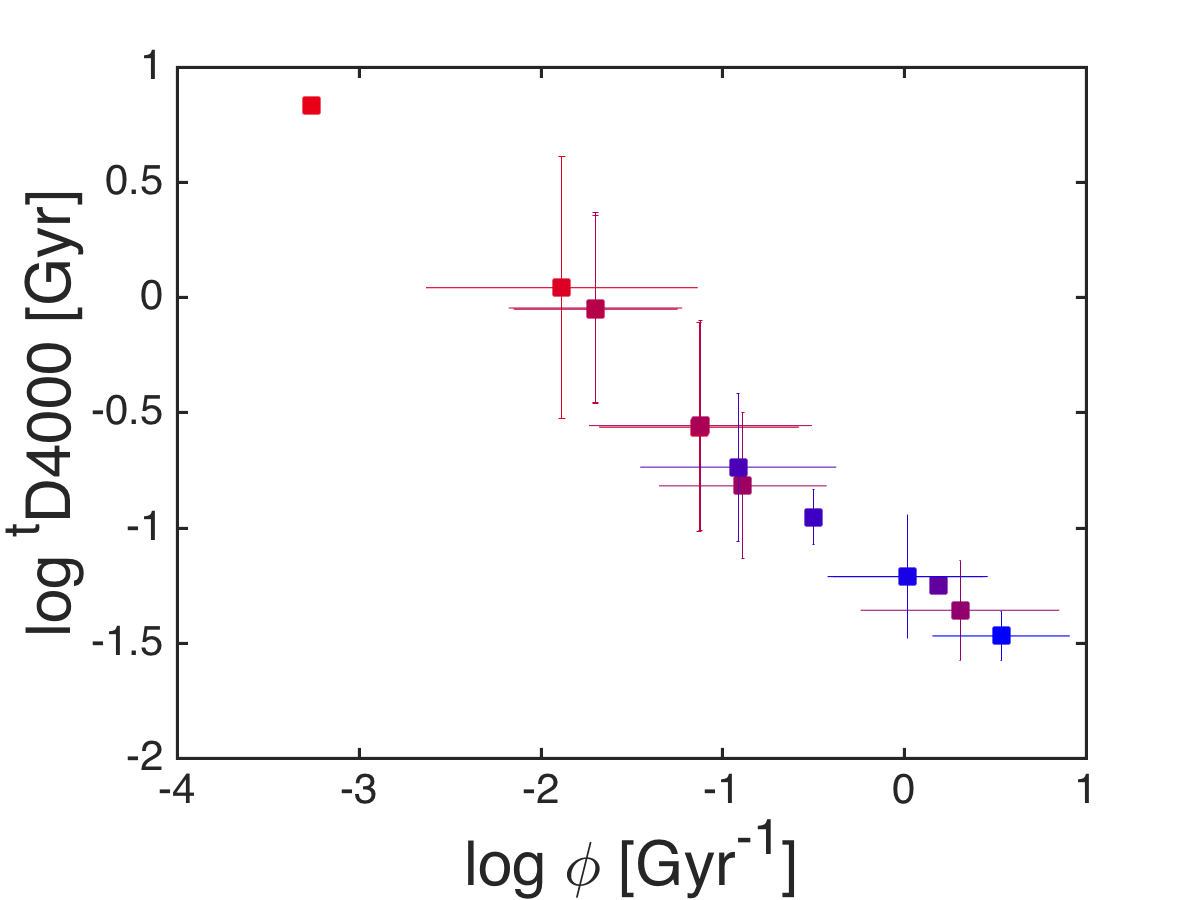
\includegraphics[width=\textwidth]{../image_paper2/1d/f1.png}
        \end{subfigure}
        \hfill
        \begin{subfigure}[b]{0.3\textwidth}
            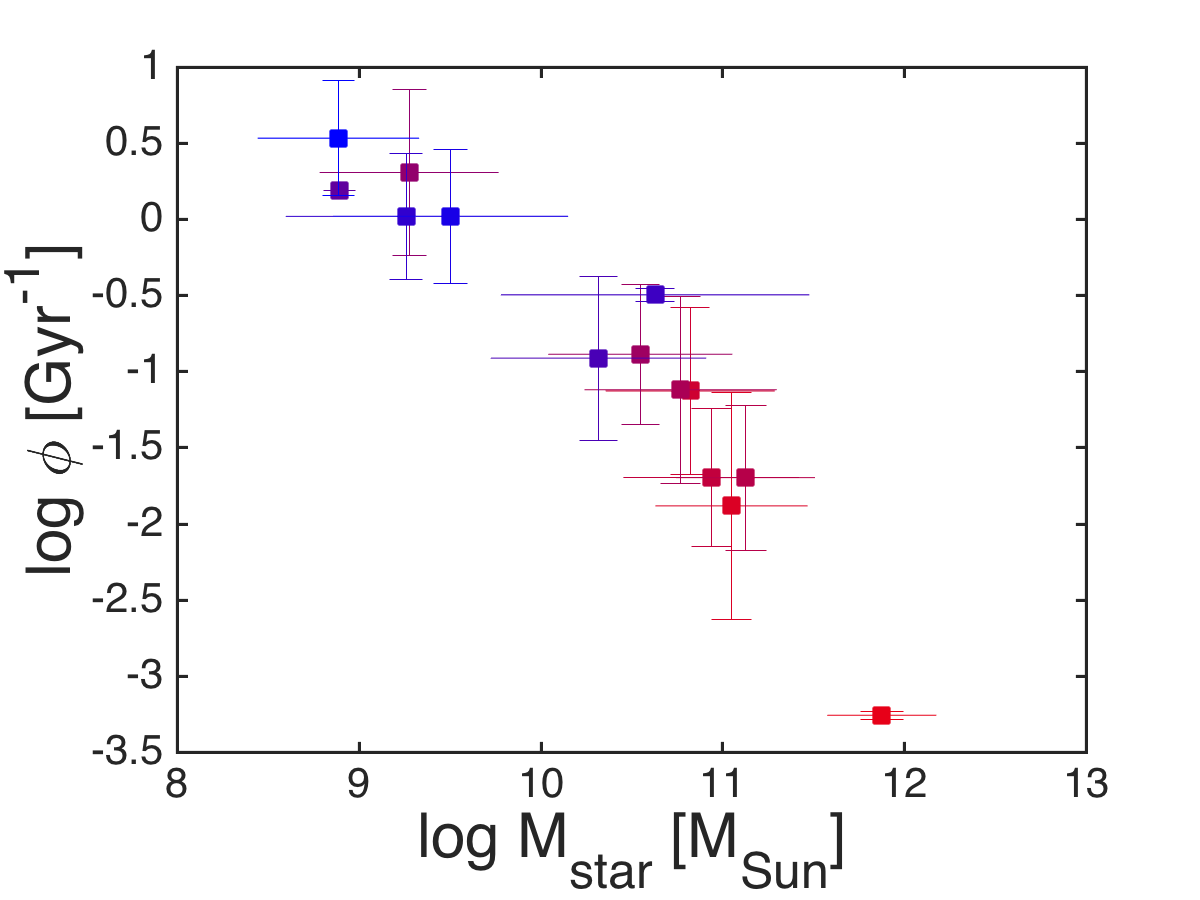
\includegraphics[width=\textwidth]{../image_paper2/1d/f2.png}
        \end{subfigure}
        \hfill
        \begin{subfigure}[b]{0.3\textwidth}
            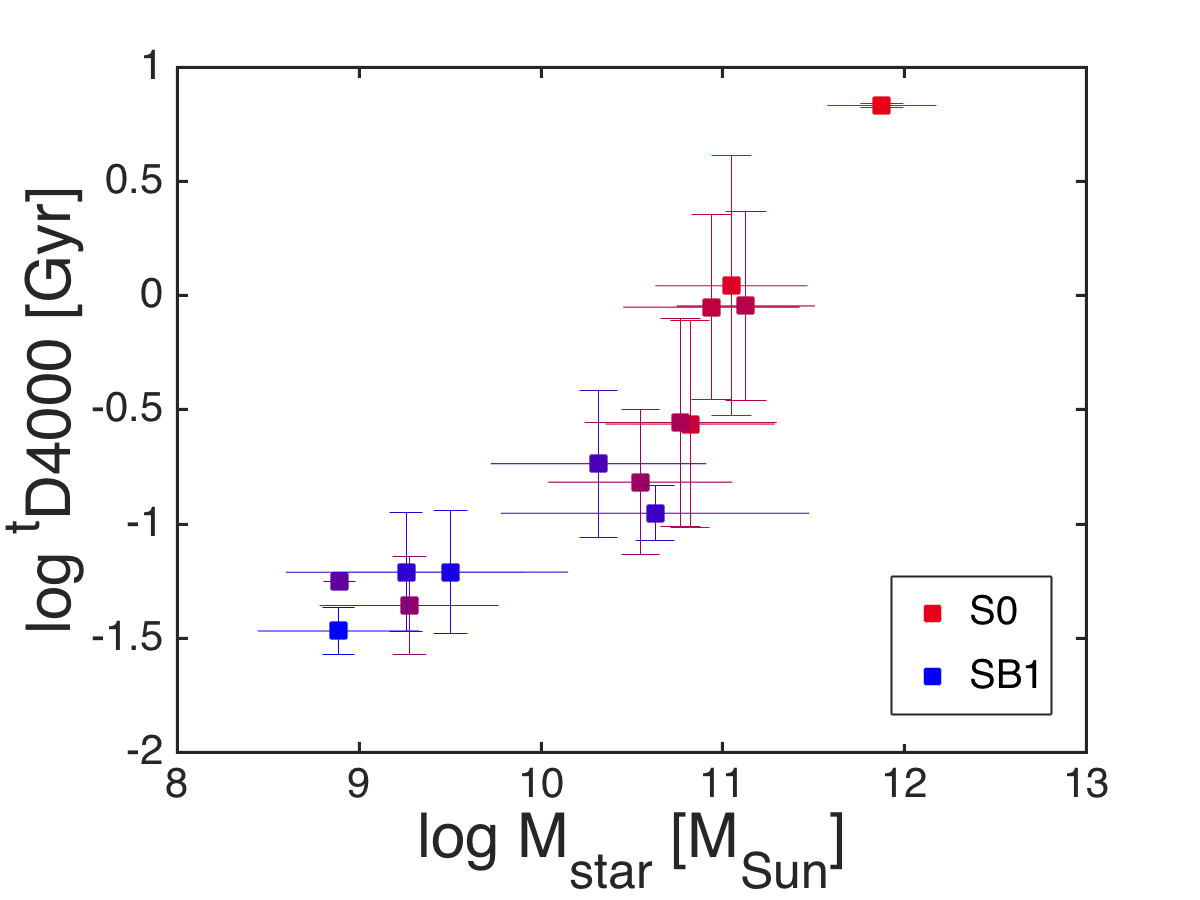
\includegraphics[width=\textwidth]{../image_paper2/1d/f3.png}
        \end{subfigure}
        \hfill
        \begin{subfigure}[b]{0.3\textwidth}
            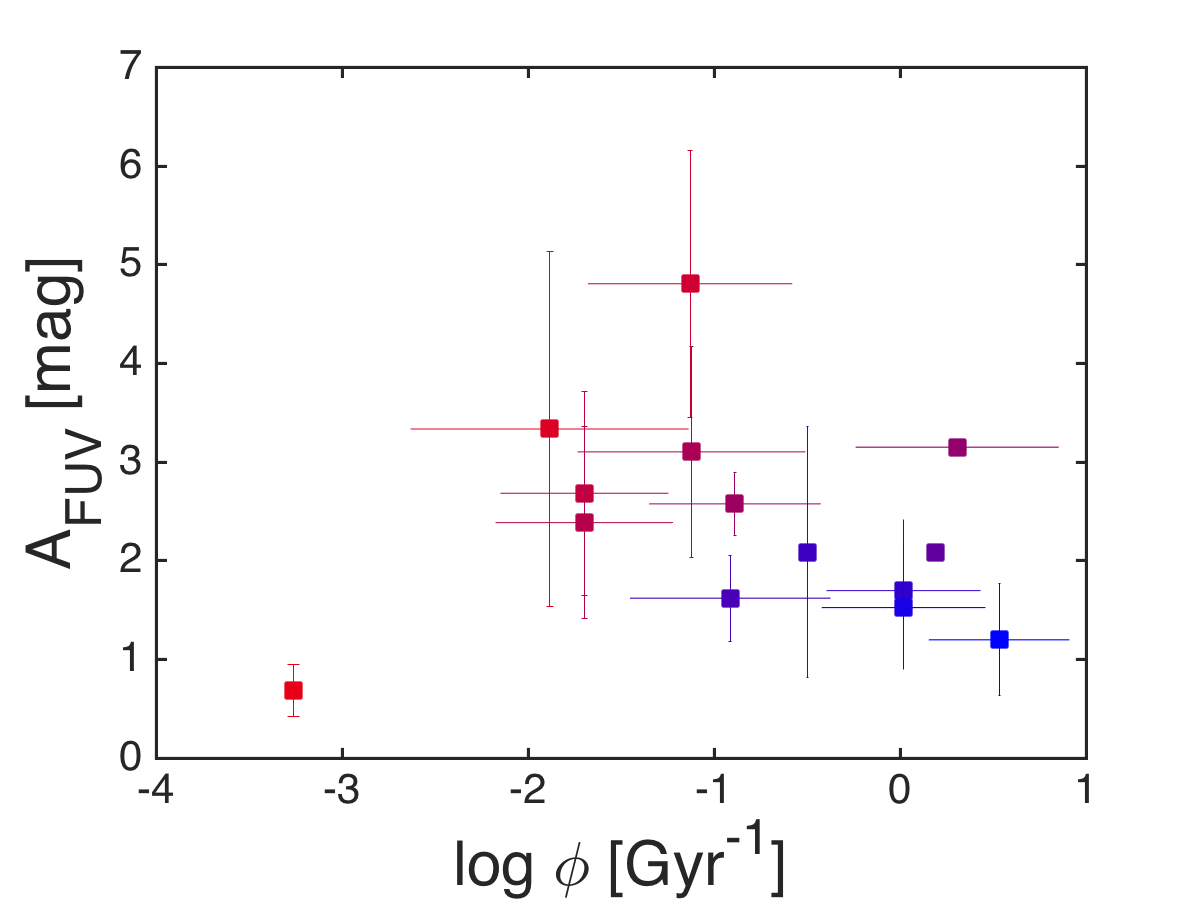
\includegraphics[width=\textwidth]{../image_paper2/1d/f4.png}
        \end{subfigure}
        \hfill
        \begin{subfigure}[b]{0.3\textwidth}
            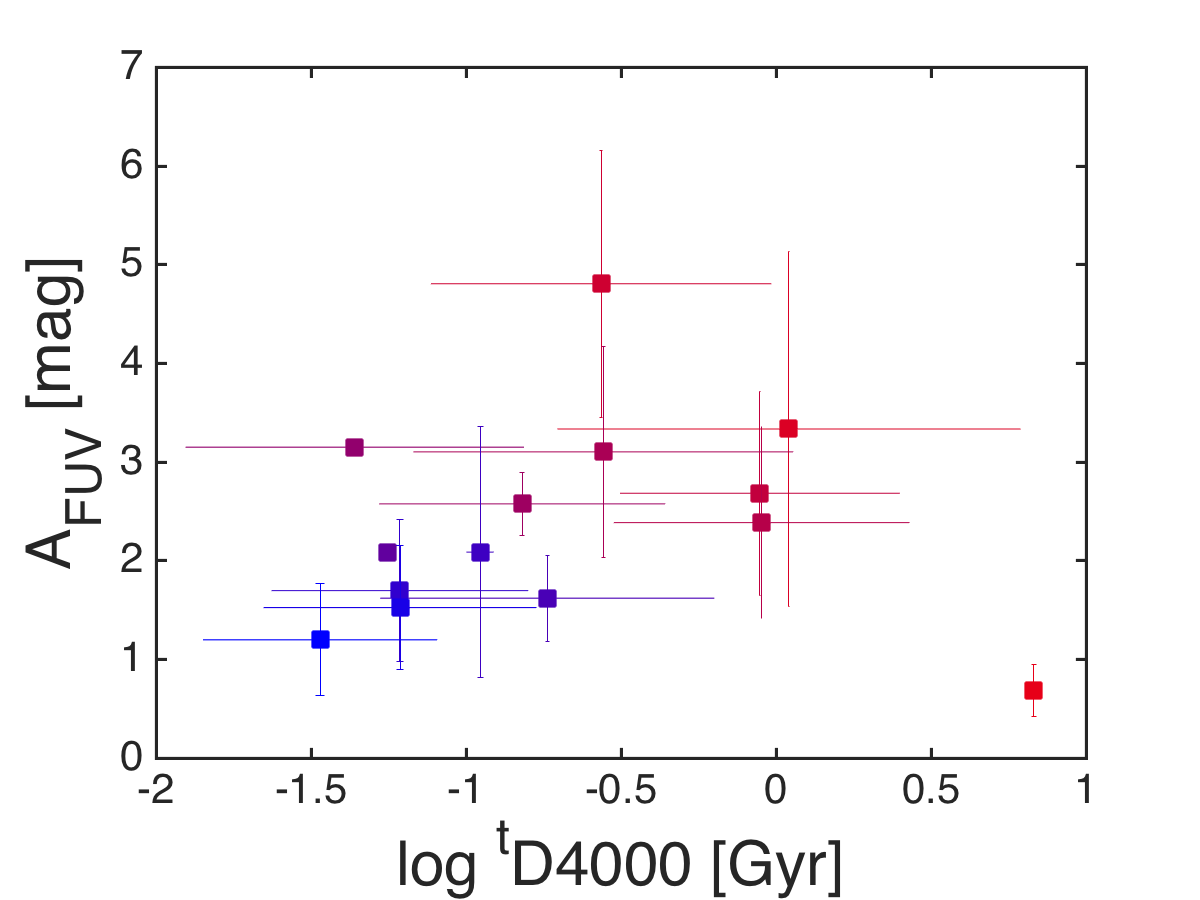
\includegraphics[width=\textwidth]{../image_paper2/1d/f5.png}
        \end{subfigure}
       \hfill
        \begin{subfigure}[b]{0.3\textwidth}
            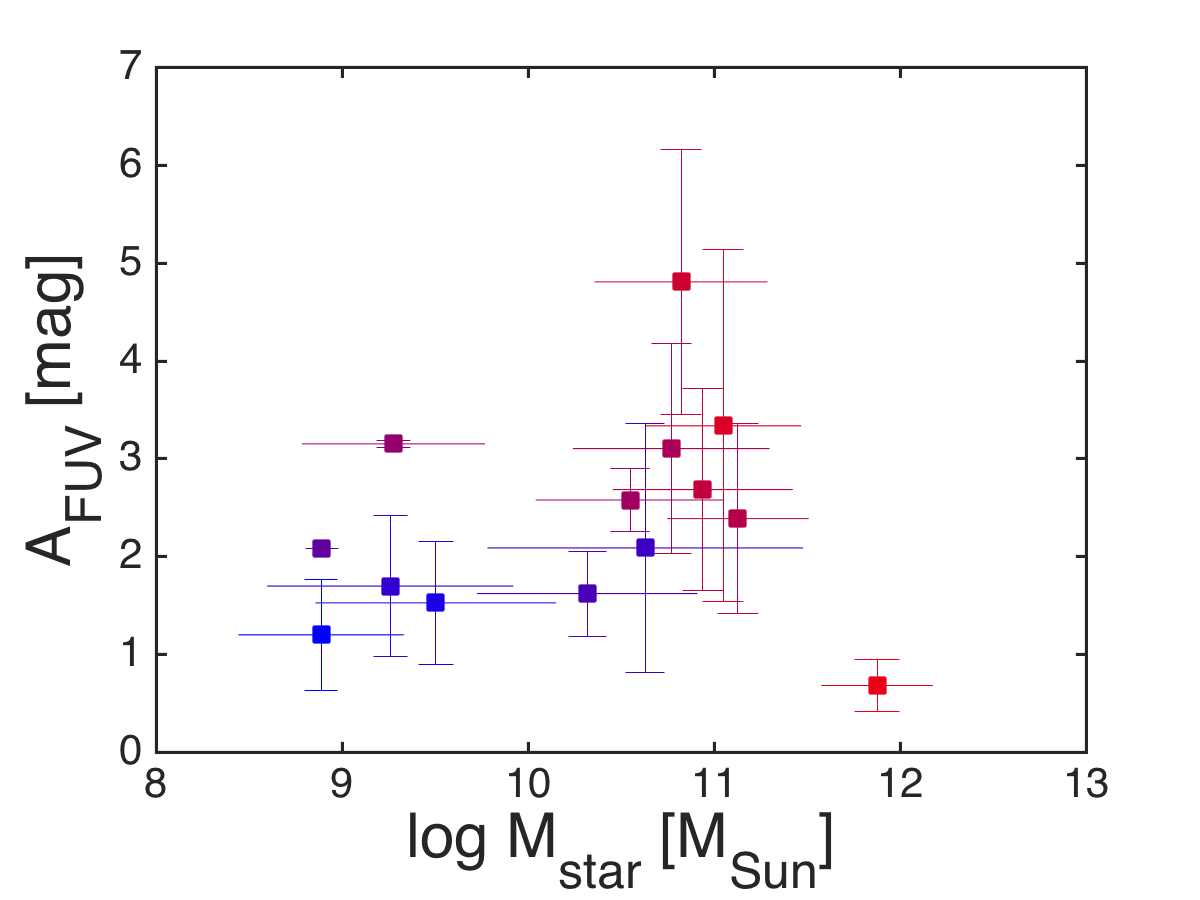
\includegraphics[width=\textwidth]{../image_paper2/1d/f6.png}
        \end{subfigure}
        \caption[Relations between properties of the clustered galaxies]{From top to bottom: Correlation between age (t$_{\rm {D4000}}$) and sSFR ($\phi$), sSFR and stellar mass, age (t$_{\rm {D4000}}$) and stellar mass, and A$_{\rm {FUV}}$ with sSFR, age (t$_{\rm {D4000}}$) and stellar mass. Points show the median values of these properties of galaxies in $1\times22$ network and error bars are the standard deviation of the median values. colours shows the type of the galaxies in the new classification. The most pure red colour shows E type galaxies and the most blue one indicates the SB1 galaxies. The other colours depend on how much they are close to red or blue show that the galaxies are quiescent or starburst.}
        \label{fig: props_vs_props}
    \end{figure}
        
        In order to compare our classifications with previous work, we produced similar plots to the ones in both \citetalias{Noll09} and \citetalias{Hossein12} (Fig.~\ref{fig: props_vs_props}).
        In Fig.~\ref{fig: props_vs_props}, the data points are median values of the properties of the galaxies in each neuron in Fig.~\ref{fig: 1by22V}, and error bars show the standard deviation of those properties.
        The colours show the galaxy types, where B type galaxies are shown with red and SB1 types are shown with blue.
        The redder the colour, the more similarity with quiescent galaxies, while the purple to blue colours show more similarity to starburst galaxies.
        Since in this method we allow galaxies to occupy classes in between the original \citetalias{Kinney96} templates, we have more than 12 colours in Fig.~\ref{fig: props_vs_props}.
        The purple point in the middle of the blue points in Fig.~\ref{fig: props_vs_props} corresponds to galaxies with spectra similar to type Sc: the shape of their spectra indicates that they are old galaxies with high sSFR.
        
        The upper panels in Fig.~\ref{fig: props_vs_props} show the same relations as \citetalias{Noll09} and \citetalias{Hossein12}, but with tighter correlation than those two, in all three plots.
        As mentioned in both \citetalias{Noll09} and \citetalias{Hossein12}, galaxies with smaller mass tend to be younger and more active.
        Fig.~\ref{fig: props} shows similar results: younger and more active galaxies have less stellar mass and more f$_{\rm {burst}}$.
        From older to younger galaxies, the colour of the points changes from red to blue, which shows a good correlation with their spectral type.
        %for more details discussion on these correlations, we encourage readers to read \citetalias{Noll09} and \citetalias{Hossein12}.
        
        \citetalias{Noll09} studied a correlation between A$_{\rm {FUV}}$ and other properties of galaxies and showed that the attenuation has no dependence on the specific star formation or age.
        In contrast to \citetalias{Noll09}, we find a correlation between A$_{\rm {FUV}}$ and these two parameters, shown in the lower panels of Fig.~\ref{fig: props_vs_props}.
        The general trend of the correlation between A$_{\rm {FUV}}$ and sSFR in Fig.~\ref{fig: props_vs_props} is similar to the trend found by \cite{Dale07}.
        They used IR luminosity to UV luminosity ratio (L$_{IR}$/L$_{FUV}$) as a measure of A$_{\rm {FUV}}$ and compared it with sSFR for all 75 galaxies in the SINGS survey.
        They found that for quiescent galaxies (E, S0 and S0/a ), L$_{IR}$/L$_{FUV}$ (or A$_{\rm {FUV}}$ ) correlates with sSFR, and for spiral galaxies, there is an anticorrelation between L$_{IR}$/L$_{FUV}$ and sSFR.
       Since our sample has no E-type galaxies, we cannot confidently show the same correlation between A$_{\rm {FUV}}$ and sSFR. 
        However, it is clear in Fig.~\ref{fig: props_vs_props} that A$_{\rm {FUV}}$ increases with increasing sSFR in the S0 and Sa types.
        The correlation in the other types of galaxies is very similar to the one shown by \cite{Dale07}.
        Both \cite{Dale07} and \citetalias{Noll09} argued that these apparent trends can be a result of the dependence of star formation history on L$_{IR}$/L$_{FUV}$.
        Whether this dependence is real or not, our results here show that using self-organizing maps can separate spectra of galaxies in such a way that the characteristics of each of these groups are in agreement with the general picture of the galaxy evolution.
      
    \subsection{Two-Dimensional Self-Organizing Maps}
    \label{sec: 2D}
    The one-dimensional networks are great tools to categorize the spectral types of galaxies and monitor the changes of properties of galaxies with category.
    However, each neuron in these networks is limited to be connected to one other neuron in each direction.
    In a 2D network, each neuron can have more than two immediate neighbours, providing a more complete pictures of relations between each spectral type.
    As described in Section~\ref{sec: method_somz}, one of the main advantages of the SOM is that when the weight of one neuron is adjusted after finding the best matching unit, the weight of the whole map will be changed.
    This quality of the SOMs provides a unique opportunity to analyse 2D networks using two approaches. 
    At first, as in the 1D SOMs, we assumed that all the galaxies must have spectra similar to any of the 12 templates in Fig.~\ref{fig: k96}.
    In this case, we can categorize spectra of other galaxies based on those 12 types.
    In the second approach, we trained networks with the assumption that there might be completely different types of galaxies not encountered before.
    This approach can be used to trace and recognize the outliers, which could include galaxy types that are not presented in the \citetalias{Kinney96} templates.
    To execute the second approach, we used the {\textsc selforgmap} library in the {\textsc matlab}.
    Unlike the {\textsc newsom} library which the ordering step neighbourhood distance is set by default (although in an SOM it should be a free parameters), in the {\textsc selforgmap} we can change this value.
    Using the {\textsc selforgmap} code, based on the size of a map and the ordering step neighbourhood distance, we can arrange that the data spread all over the SOM or sit close together, allowing room for outliers.

    To get the best result from both methods, we should have SOMs with ``enough"  neurons to give any new types of galaxies a chance to find their places in the map.
    ``Enough neurons" is a vague statement, but as mentioned in the Section~\ref{sec: method_somz} the size of SOMs is arbitrary and depends on the size of the input data and the kind of information needed from the SOMs.
    Since the training dataset (the \citetalias{Kinney96} templates) has 12 members, we assumed a SOM with size of $8\times8$~would be a good start.
    We then increased the size of the SOM to find the highest size suitable for the training sample.
    We noticed that very few changes occurred after the SOMs were grown to a size greater than $12\times12$, so we used this as the maximum size.
    
    \begin{figure}
        \begin{subfigure}[b]{0.45\textwidth}
            \centering
            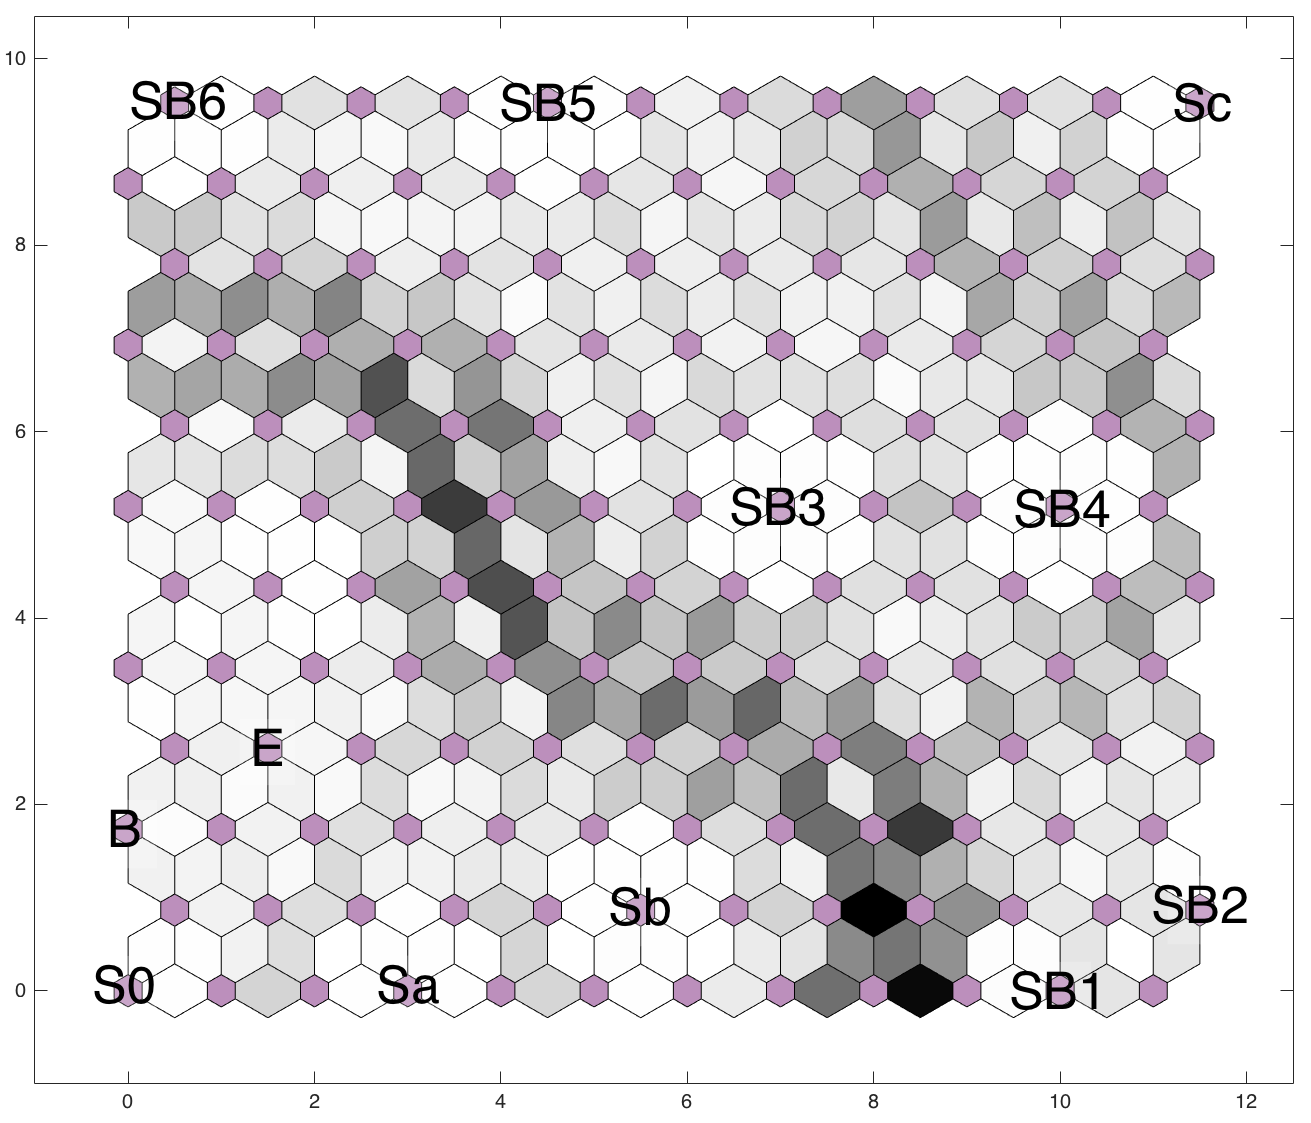
\includegraphics[width=\textwidth]{../image_paper2/2d/dist_12_by_12.png}
        \end{subfigure}
        \hfill
        \begin{subfigure}[b]{0.45\textwidth}
            \centering
            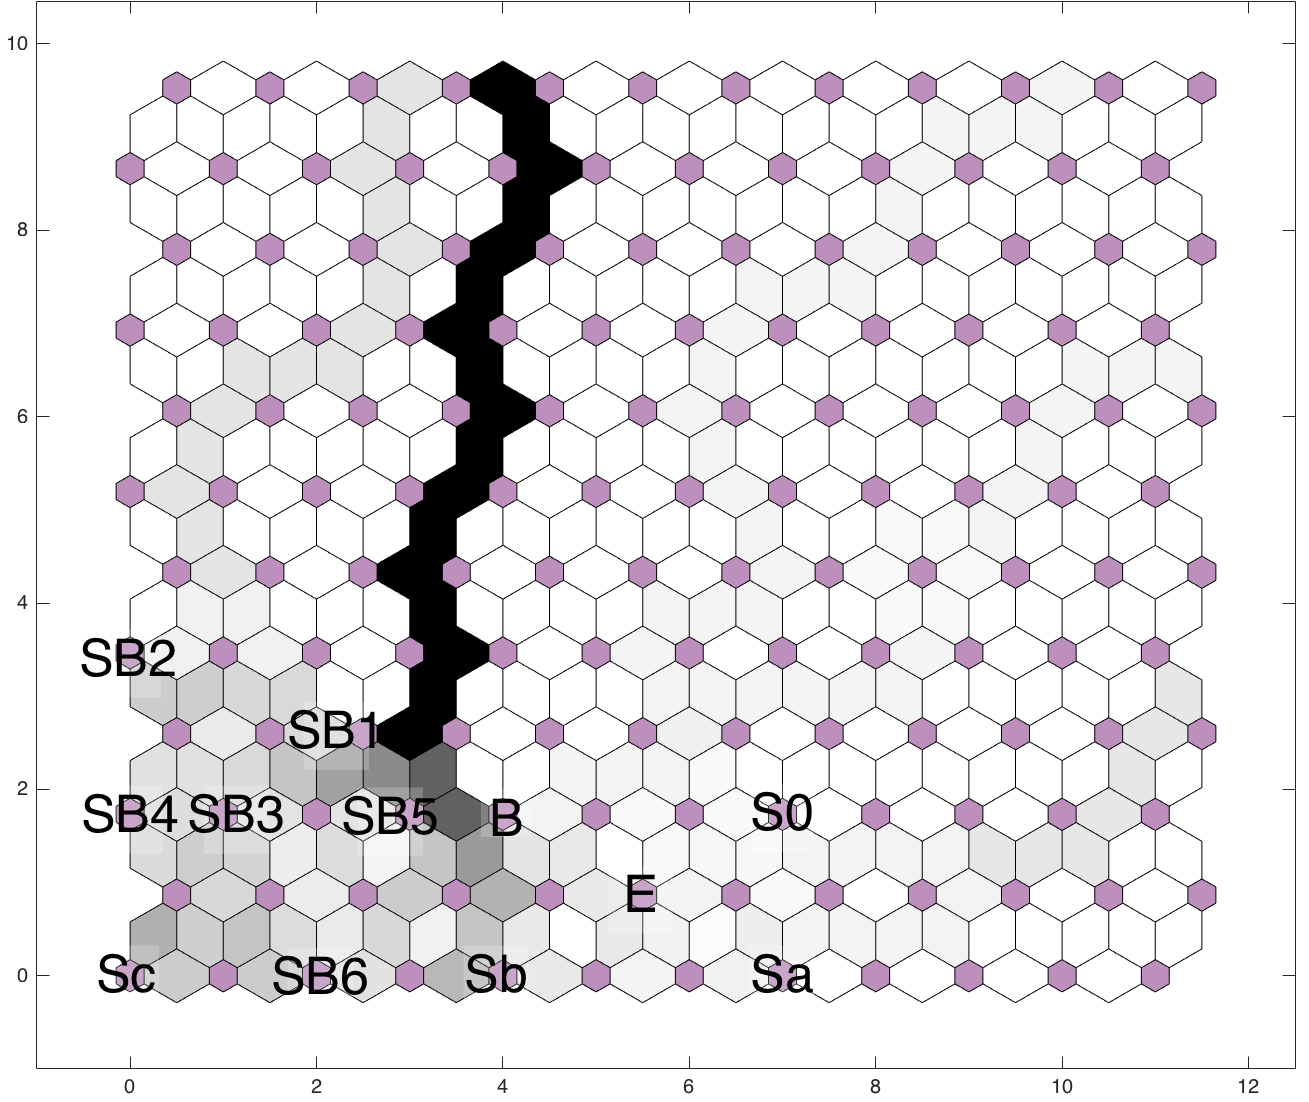
\includegraphics[width=\textwidth]{../image_paper2/2d/dist_12_by_self_org_res12.png}
        \end{subfigure}
        \hfill
        \begin{subfigure}[b]{0.45\textwidth}
            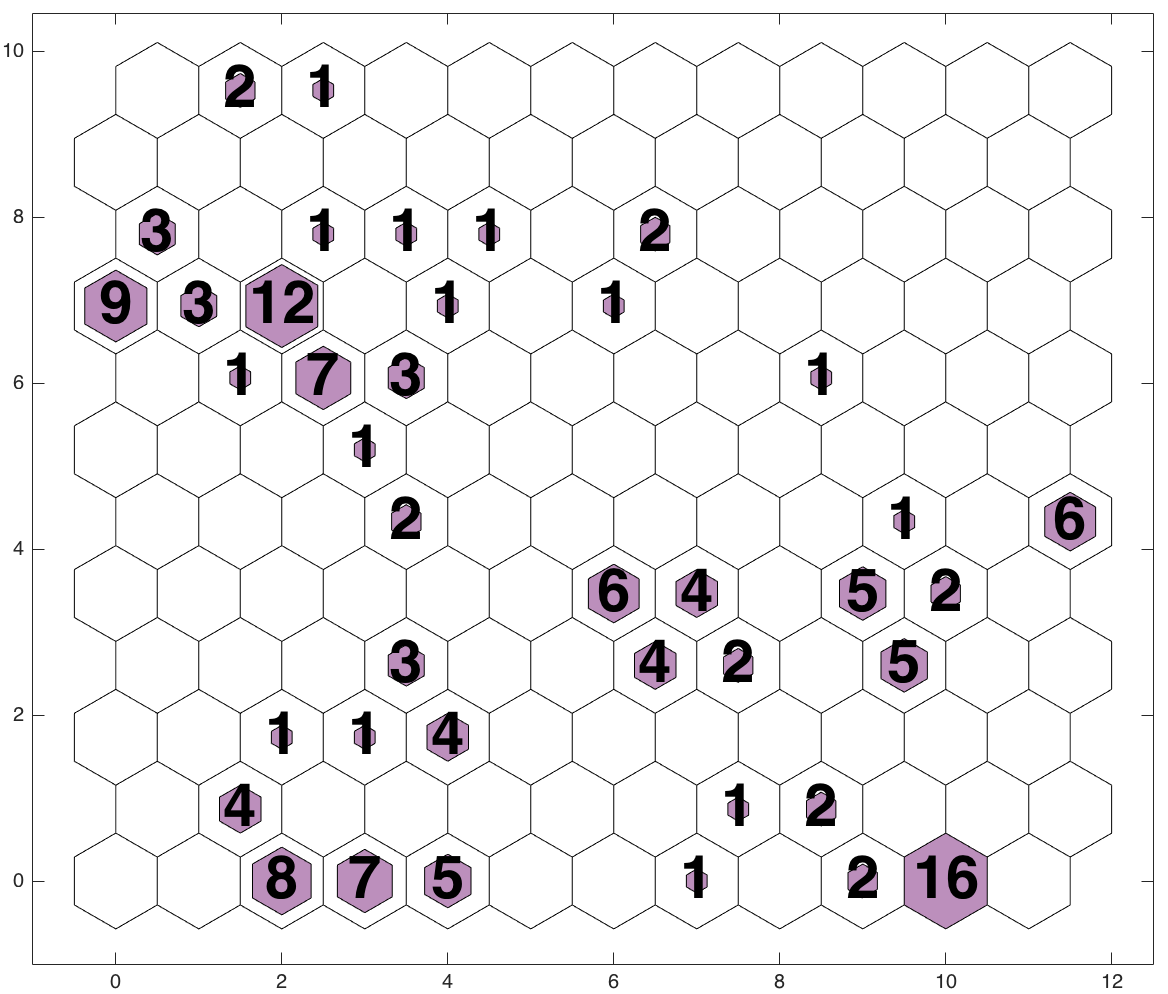
\includegraphics[width=\textwidth]{../image_paper2/2d/hit_v_12_by_12.png}
        \end{subfigure}
        \hfill
        \begin{subfigure}[b]{0.45\textwidth}
            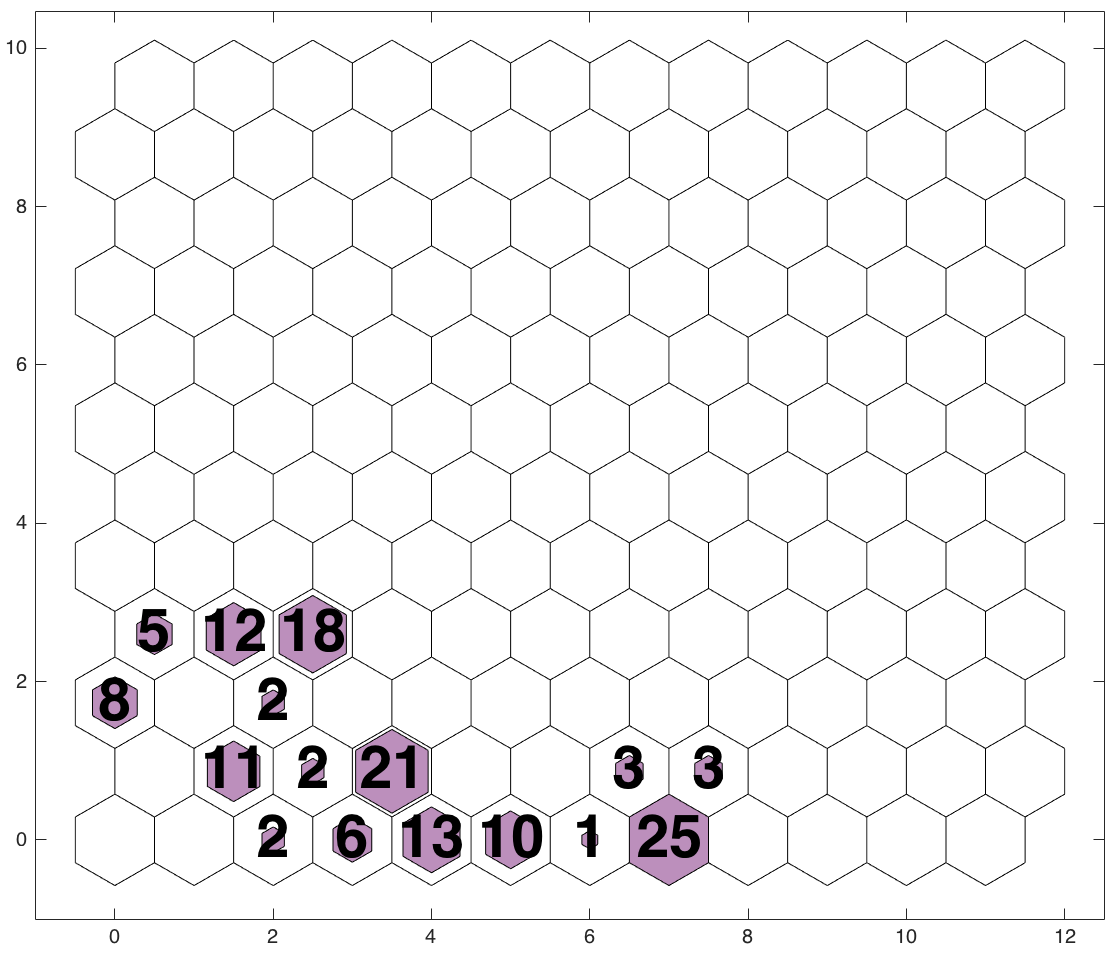
\includegraphics[width=\textwidth]{../image_paper2/2d/hit_v_12_by_self_org_res12.png}
        \end{subfigure}
        \caption[$12\times12$ two-dimensional self-organizing map results]{$12\times12$~2D SOM results. Upper panel: SOMs trained using the \citet{Kinney96} templates. For training 2D SOMs two different approaches were considered: either only 12 types of galaxies exist (left) or not (right). Lower panel: classifying the galaxies from \citetalias{Hossein12}, using the trained networks shown in the upper panels. From the lower right panel, we can see that there are no outliers in the galaxies from \citetalias{Hossein12}, and we can use the map in the lower left panel as a final clustering result for the \citetalias{Hossein12} galaxies.}
        \label{fig: 12by12}
    \end{figure}
    
    The upper left panel in Fig.~\ref{fig: 12by12} shows the SOM results from the first approach. 
    Since we considered that spectra of all galaxies can be categorized using the \citetalias{Kinney96} templates, the galaxies were placed all over the map.
    Using this network to categorize any set of spectra forced the spectra to be either in the same neurons as the \citetalias{Kinney96} templates or in the neurons between them.
    In the map shown in the upper right panel in Fig.~\ref{fig: 12by12}, the \citetalias{Kinney96} templates are in a small region. This provides enough freedom for the spectra of galaxies to be placed everywhere in the map, even far away from the templates.
    
    
    In the upper left part of the map in Fig.~\ref{fig: 12by12}, although galaxies have more ways to be separated, they were separated in two main groups.
    There is a distinguishable strip of grey, dark grey and in some cases black colour in the map:
    this strip separates quiescent galaxies from starburst ones.
    The lower map shows that 5 of the neurons on the left side of the strip are full. 
    These five neurons are the same as the ones on the left hand side of Fig.~\ref{fig: 1by2T} (quiescent galaxies),
    the only difference being that in this map they have more space to be separated from each other.
    When we use this network to categorize the spectra of galaxies, any galaxy placed on the left hand side of the strip is a quiescent galaxy and any one placed on the right side of the strip is a starburst one.
    The decision about what sub-type of quiescent or starburst galaxy is based upon its relative position to each type in the SOM.
    
    As in the other map, in the upper right panel of Fig.~\ref{fig: 12by12}, galaxies are generally divided into two main groups.
    The border between the quiescent galaxies and the starburst ones is the black strips in the middle of the map,  ending with the bright grey colour at the bottom of the map in the fifth neuron.
    In this network, neurons in the right side of the strip represent the quiescent galaxies and the neurons in the left side represent the starburst ones. 
    When categorizing a new set of spectral types, if the new spectra are similar to the \citetalias{Kinney96} template all of them will be placed in the bottom of the map, but if there are different type of galaxies, they would sit in any other neurons in the map.
    In large datasets, one can easily use this network to figure out whether there is any of new type of spectra (or any outliers) in the datasets. 
    Since the networks are already available, this procedure should be quick and easy for big datasets.
    
    We used both 2D networks to categorize the \citetalias{Hossein12} galaxies and the results are shown in the lower panels of Fig.~\ref{fig: 12by12}.
    In the lower right map in Fig.~\ref{fig: 12by12}, all galaxies are placed in the bottom part of the map and we can conclude that in the \citetalias{Hossein12} sample there are no outliers or spectra with very different from the \citetalias{Kinney96} templates.
    The lower left map of Fig.~\ref{fig: 12by12} shows the \citetalias{Hossein12} galaxies categorized based on the network in the upper left of Fig.~\ref{fig: 12by12}. 
    Comparing this categorization with the 1D one from Fig.~\ref{fig: 1by22V}, we can see that only 23 galaxies correspond exactly to \citetalias{Kinney96} types.
    Using 2D maps results in categorizing galaxies into more intermediate type than in 1D maps.
    In both lower maps in Fig.~\ref{fig: 12by12}, most galaxies are in the quiescent side of the SOM, which was predictable from the results in Sec.\ref{sec: 1Dv}. This does not imply that in general there are more quiescent galaxies at higher red-shifts but rather is a selection effect from the fact that those galaxies had more reliable redshift estimates.
    
    Although for ease of presentation this paper first discusses 1D networks and continues to 2D networks, we suggest that users of SOMs for galaxy spectral classification should use 2D networks first. These can be used as a first step with networks similar to the upper left map in Fig.~\ref{fig: 12by12} to identify outliers in the sample.


%----------------------------------------------------------------------------------------
%----------------------------------------------------------------------------------------
%----------------------------------------------------------------------------------------
%Summery
%----------------------------------------------------------------------------------------
%----------------------------------------------------------------------------------------
%----------------------------------------------------------------------------------------
\section{Summary and Future Applications}
\label{sec: summary_SOMZ}

Self-organizing maps can be used to classify celestial objects (e.g. stars, quasars, spectra of galaxies, light curves, etc.)
Galaxy spectra can be classified in various networks with different sizes/dimensions based on the information needed from the data. 
If a broad and general classification is required, networks can have one dimension with a few neurons.
If one needs more detailed classifications, a higher number of neurons should be used.
Since self-organizing maps do not include the uncertainty of input parameters, sometimes too much attention to detail can cause problems in classifications. 
%Some small differences could easily be the result of atmosphere fluctuation or other instrumental or observational problems. 
When using the SOM method, one should consider whether small differences between objects are physically meaningful when separating two groups from each other.

We used SOMs to classify the template spectra of \citetalias{Kinney96}, made from galaxies with known morphological type, and created networks with different uses.
By varying the size of the networks, we found the relative similarity between the \citetalias{Kinney96} template classes.
A one-dimensional network with 22 neurons was needed in order to
separate all 12 \citetalias{Kinney96} spectra; we concluded that \citetalias{Kinney96} types B and E, and types SB1 and SB2, are very similar to each other.
We also showed that networks generated with the SOM method can be used to easily identify new types of spectra in large surveys.

A sample of 142 high red-shift galaxies from \citetalias{Hossein12} was used to test the trained networks.
%One of the main criteria to choose a test sample is that the test sample must have fluxes in exactly the same wavelengths of the training sample.
The test results showed that using SOMs can allow identification of galaxies with spectra similar to two or more morphological types.% but not exactly the same as one of them.
The freedom of having in-between types is one of the main differences between supervised and unsupervised artificial neural networks.
\citetalias{Hossein12} used a supervised training method to train networks with \citetalias{Kinney96} spectral templates and classify the same sample of 142 galaxy spectra;
however, they could not classify 37 out of 142 spectra.
The unsupervised method used in this project was able to classify all 142 spectra in the sample
as belonging to one of the morphological types introduced by \citetalias{Kinney96} or a class in between those types.

The properties of the galaxies in the test sample using the new
classification were found to more tightly correlate in mean values of age, specific star formation rate, stellar mass, and far-UV extinction than in previous studies. 
The properties of the galaxies in each group are in good agreement with their morphological types.

Two-dimensional networks can be used to find the relations of the neurons and classifications in more details.
The sample galaxies have more freedom to be categorized, and only 23 of them occupy exactly the same neurons as the \citetalias{Kinney96} template spectra (in one-dimensional networks this number was 56).
Additionally, by using two-dimensional networks we showed that we do not have any outliers in the sample galaxies.


\addcontentsline{toc}{section}{Bibliography}
\bibliographystyle{apj.bst}
\bibliography{ref_paper2.bib}

\chapter{Conclusions \& Future Work}
\label{ch: summary}
 %General
The formation of stars is one of the fundamental factors in the formation and evolution of galaxies.
Measuring the star formation rate and its variation through time helps us to learn about how a galaxy forms and evolves.
Many efforts have been made to find a universal law for the rate at which stars form.
In order to find a universal law, finding a method to measure SFR accurately is the first step.
Then correlations between SFR and other properties of galaxies must be investigated.
Afterward, each law has to be tested in various environments to confirm its universality.
Therefore, we need high quality data and good statistical methods to test the laws.

It has been well established that to form stars, gas is the main ingredient.
However, the relation between SFR and different tracers of gas mass (atomic, molecular, or total gas) changes in different type of galaxies.
Relations between stellar mass, metallicity and SFR are not clear and there are fewer studies of these than of the relation between SFR and gas mass.
The dependence of SFR on other properties of galaxies such as morphology and dust mass have been tested as well, but there is no SFR law that considers all of the above quantities together.
The Kennicutt-Schmidt law ~\citep{Schmidt59, Kennicutt98b} was the first empirical star formation law, suggesting that SFR and molecular gas have a logarithmic correlation with each other. 
However, after many years and studies, there is still an ongoing question of whether it is a universal law or not.
\citet{Shetty13} showed that, besides the physical and environmental effects, fitting methods also change our perspective of the K-S law.
Extended version of the K-S law were introduced by adding the effect of stars (extended Schmidt law; introduced by ~\citealt{Shi11}) or metallicity (Krumholz law; introduced by ~\citealt{Krumholz09}).
Compared to the K-S law, the extended Schmidt law and Krumholz law are relatively recently introduced and still need to be tested with diverse statistical methods on different scales (local and global), with various morphological types and in both nearby and high-redshift galaxies.

%Chapter 2
Spatially resolved images of the Andromeda galaxy (M31) cover different types of environments within a galaxy: high or low stellar surface density, gas mass, and metallicity.
These images permit us to examine star formation laws in detail, in various environments.
In Chapter~\ref{ch: paper1}, we investigated three star formation laws in M31 on both local and global scales in order to determine which of these laws describe M31 data more accurately.
To achieve this goal, we produced maps of surface density of SFR, gas mass, stellar mass and metallicity of the galaxy.
We created SFR maps using three SFR indicators: a combination of the FUV and 24~\um emission, a combination of the \halpha and 24~\um emission, and TIR luminosity. 
Using a combination of the FUV and 24~\um emission, we determined the total SFR for M31 to be $0.31\pm 0.04$~M$_\odot$~yr$^{−1}$.
We measured the ISM gas mass using molecular gas only, atomic gas only and the total gas.
We confirmed that the extended Schmidt law holds in M31 for local regions and the effect of stellar mass in regions with low gas density is even more pronounced. 
By applying both the K-S law and the extended Schmidt law on all SFR maps and gas maps, we concluded that changes in SFR tracer do not affect these laws as much as changes in gas tracer.
Our fitting results show that in regions with higher star formation rate, power laws are more in agreement with other studies.
In order to examine Shetty's suggestions on the effect of fitting methods on SFR laws, we used hierarchical Bayesian regression fitting and normal regression fitting to fit SFR laws.
The results from the two different methods are dissimilar, mostly because of the ways these two methods handle the uncertainties.
The measured SFR by the Krumholz law did not match with the observed data in M31.
By performing statistical tests, we showed that there is no strong correlation between metallicity and SFR in M31.


%Chapter 3 
For the remainder of this thesis we used a machine learning method to have a fresh look on star formation and its relation to other properties of galaxies.
We chose the self-organizing map algorithm as our data mining method because of its ability to classify results and show the morphology of data, simultaneously.
The amount of observational data and derived quantities for M31 is enough to make this galaxy a good target for machine learning studies.
Therefore, in Chapter~\ref{ch: paper3} we applied the self-organizing map algorithm on observational data from M31.
We used observational data and derived quantities of 10 regions in M31, which were chosen due to the availability of mid-infrared spectroscopy for those regions.
Therefore, we were able to focus on relations between SFR and interstellar medium components, specifically polycyclic aromatic hydrocarbons (PAHs).
Using a network with 2 neurons, we divided the data into two major groups.
By comparing data from these groups, we found correlations within groups that otherwise would not have been seen.
In one of the groups, the flux from PAHs showed strong anti-correlations with \halpha, \sii, \oiii~and IRAC 5.8~$\mu$m emission, stellar mass and radiation hardness index.
We found two reasons for PAHs to anti-correlate with optical emission and RHI.
First, the harder radiation field could make the size of \hii~regions bigger and the size of photo-dissociation regions smaller, causing more \halpha~emission and less PAH emission.
Second, since optical emission was not corrected for dust extinction, dustier regions would have less observed optical emission.
Since for 10 regions in M31 we needed at least 14 neurons to separate all 10 regions from each other, we concluded that some of these 10 regions have very similar properties.
Using subsets of the data we generated various two dimensional networks.
The networks created by the subsets showed that, except for PAH-only subsets, region 10, which is located in the bulge of M31, becomes isolated.
The network from the PAH-only data is the only network with no isolated regions, which means that, despite differences in underlying physical conditions in different regions, PAHs in M31 are very similar.
We created another network using the same set of M31 observations that were available for M101.
Using subsets of data, we show that the SOMs can be used to predict observations for regions that lack the observational data for some quantities (e.g.\ PAH emission).
We applied this network to the M101 observations and showed that regions with relative similarity to M31 data were placed in the same neurons.
Therefore, we can use these networks to predict properties of other galaxies.


%chapter 4
In Chapter~\ref{ch: paper2}, we used the self-organizing map algorithm on data from high-redshift galaxies.
We classified the template spectra of~\citet{Kinney96}, made from galaxies with known morphological type, and created networks with different uses.
Similar to the results of Chapter~\ref{ch: paper3}, since we needed at least 22 neurons to separate 12 spectral types, we concluded that some of the spectral types have very similar features (types B and E, and types SB1 and SB2 from \citealt{Kinney96}).
We showed that network generated by the self-organizing map method can be used to identify new types of spectra in large surveys.
Using the trained networks, we classified a sample of 142 galaxies from~\citet{Hossein12}.
The classification by self-organizing map allowed us to identify galaxies with SEDs similar to two or more morphological types.
Comparing our results with classifications from trained networks showed that this unsupervised method could classify all 142 spectra while the supervised methods failed to classify 37 out 142 galaxies. 
The properties of the 142 classified galaxies show better correlations in mean values of age, specific star formation rate, stellar mass, and far-UV extinction compared to the other methods.
These correlations are also in agreement with the galaxies' morphological types.

%future works and add big questions
To move forward, we would like to test star formation laws in high-redshift galaxies with the hierarchical Bayesian regression fitting method. This would allow investigation of both the effects of fitting methods on using global values for galaxies and differences in using this method on nearby galaxies and high-redshift ones.  
We could also use data mining methods to recalibrate the correlations between luminosities from star forming regions and the SFR in both nearby and high redshift galaxies.
Self-organizing maps can help us to examine our calibrations of the SFR, find their flaws and predict the SFR in distant galaxies.
Another project to continue after this thesis would be to show that self-organizing maps are good tools to predict properties of galaxies and estimate values of unobserved quantities.
Continuing the work in Chapter~\ref{ch: paper3}, we would like to obtain mid-infrared spectroscopy with more coverage in M31 and other nearby galaxies to have a higher dimensional sample for creating SOMs as well as to investigate the anti-correlation between stellar mass and PAHs.
Having these new calibrations for finding properties of galaxies and applying them to observations from recently (or soon to be) operational telescopes such as TMT, ALMA, SKA, and {\it JWST} would help us solve the mystery of how stars form and evolve in time.




\addcontentsline{toc}{section}{Bibliography}
\bibliographystyle{apj.bst}
\bibliography{western_bib.bib}



%% This adds a line for the Bibliography in the Table of Contents.
% \addcontentsline{toc}{chapter}{Bibliography}
% %% ***   Set the bibliography style.   ***
% \bibliographystyle{apj.bst} % (change according to your preference)
% %%% ***   Set the bibliography file.   ***
% \bibliography{western_bib}

% \addcontentsline{toc}{section}{Bibliography}
% \bibliographystyle{apj.bst}
% \bibliography{western_bib.bib}

%Appendices.

% %Appendices.
 \begin{appendices}
 \chapter{Appendix}
\section{SFR from H$\alpha$ plus 24 \um: procedure and result}
\label{app:halpha}

As mentioned in Section~\ref{sec:data}, we used the H$\alpha$ data from the Nearby Galaxies Survey \citep{Massey07} to create one of our SFR maps. These data cover 10 overlapping fields across the disk of M31 in broad and narrow bands and were observed between August 2000 and September 2002; we obtained them  from the NOAO Science Archive. Making a spatially resolved SFR map of M31 using H$\alpha$ emission requires removal of background and stellar emission in each field, masking out foreground stars and saturated regions, creating a mosaic of H$\alpha$ continuum-subtracted images, and finally correcting for the flux contribution to the \halpha filter from the [N II] 6583~\AA\ line.

The Nearby Galaxies survey $R$-band images were used to remove the stellar emission from H$\alpha$ using the scaling factor between fluxes in these two band passes determined by \citet{Azimlu11}. They estimated continuum emission in each H$\alpha$ image, using photometric measurements in both \halpha and R-band images, and determined the scaling factor. These images were observed from a ground-based telescope over two years' time. Consequently, there is a non-negligible sky contribution in the background which must be estimated and removed from each image in both bands. Unfortunately, there is no nearby `blank-sky' image taken with the same instrument available from which to measure the sky contribution, which makes the removal of background emission even harder. The only remaining choice is to subtract the local background for each region. However, subtracting local backgrounds from each image will result in a non-smooth background in the final mosaic image. 


\begin{figure*}
\centering
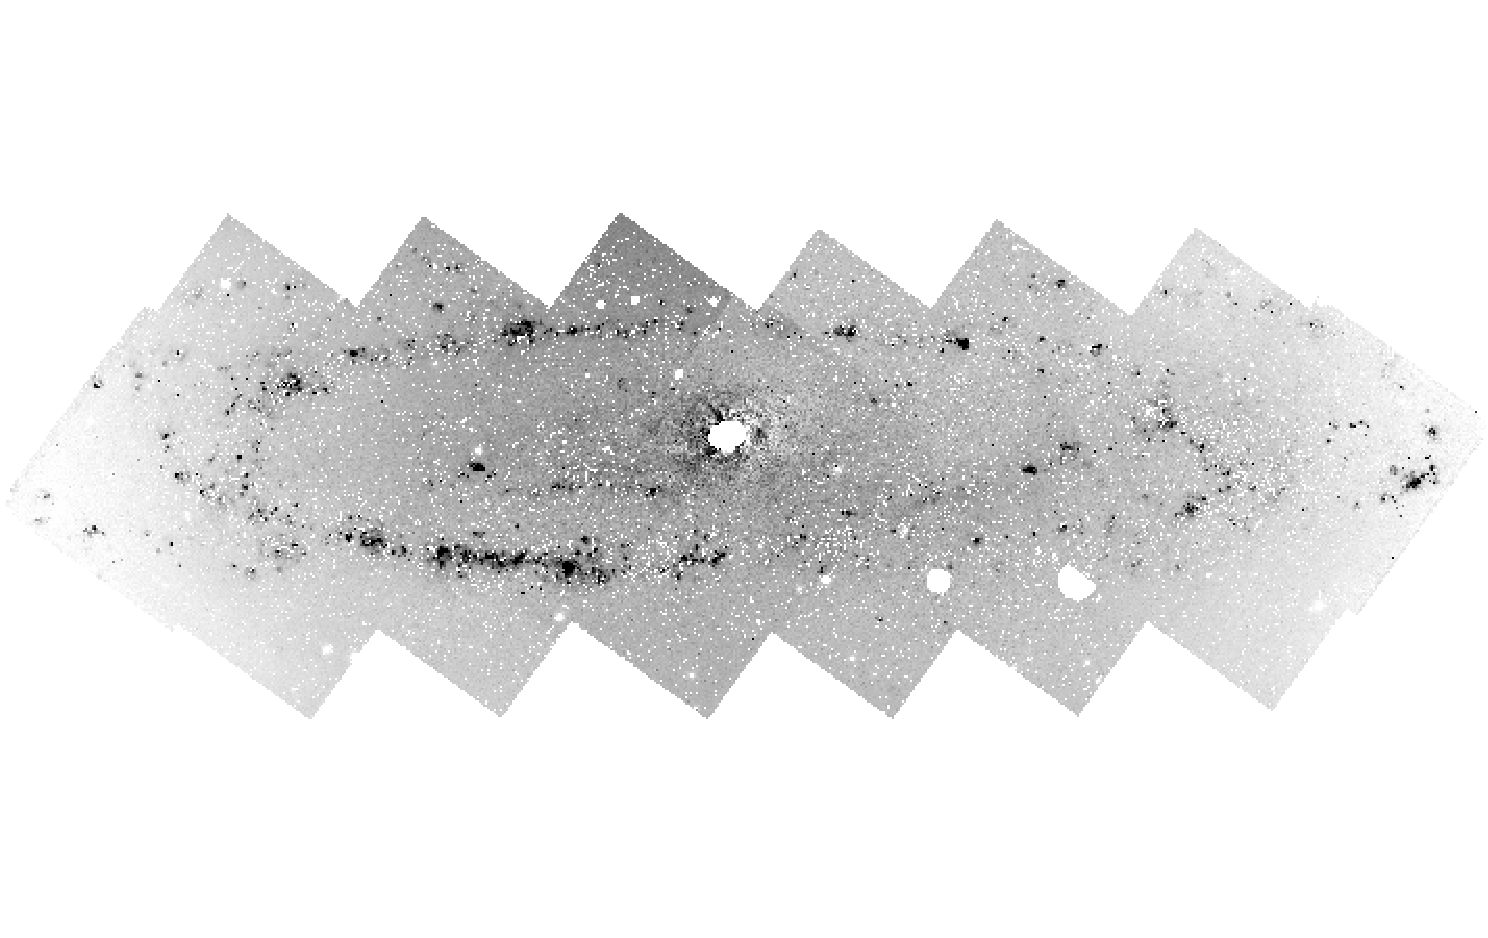
\includegraphics[width=164mm]{../image_paper1/halpha.pdf}
\caption{Mosaic created using the Montage programme from six fields of H$\alpha$ emission images of M31 from \citet{Massey07}. The resulting image from Montage was continuum-subtracted and masked for all point sources. The centre of the galaxy was masked out due to saturation of data in the continuum $R$-band image.}
\label{fig:halpha}
\end{figure*}

To create the final mosaic, first we removed the background from each region in both the \halpha and $R$-band images. The second step was to subtract the continuum from the \halpha images. Since both \halpha and $R$-band images were aligned on the same coordinate grid, for each field, the R-band image multiplied by the scaling factor was subtracted from each corresponding \halpha image. At the end, we masked out all the foreground and saturated regions which include a $10\arcmin \times 10\arcmin$ region in the centre of the galaxy. To account for the flux contribution of the [N II] emission we used the flux ratio ${\rm [NII]}/{\rm H}\alpha = 0.54$ from \citet{Kennicutt08}, and subtracted it from the \halpha map. We created the final mosaic image, Figure~\ref{fig:halpha}, using the Montage program \citep{Berriman08}.

Creating the SFR map using \halpha plus 24 \um was described in Section~\ref{sec:sfr_halpha}. In order to investigate the SFR laws, we used the same method of the fitting as Section~\ref{sec:fitting}. The fitting results using SFR(\halpha $+$ 24~\um) are more or less the same as the other two SFR tracers. The main reason for this difference is the missing data in the centre of the galaxy and the lack of smooth background in the \halpha data. Thus we did not include the SFR(\halpha $+$ 24 \um) in our final analysis.

\newpage
\section{More results from the fitting of the extended Schmidt law}
\label{app:es,figs}
Section~\ref{sec: sfl} discusses testing the extended Schmidt law and shows results for one SFR/gas tracer combination. Here we present the plots for the remaining SFR/gas tracer combinations.


\begin{figure*}
    \centering
    \begin{subfigure}[b]{0.5\textwidth}
        \centering
        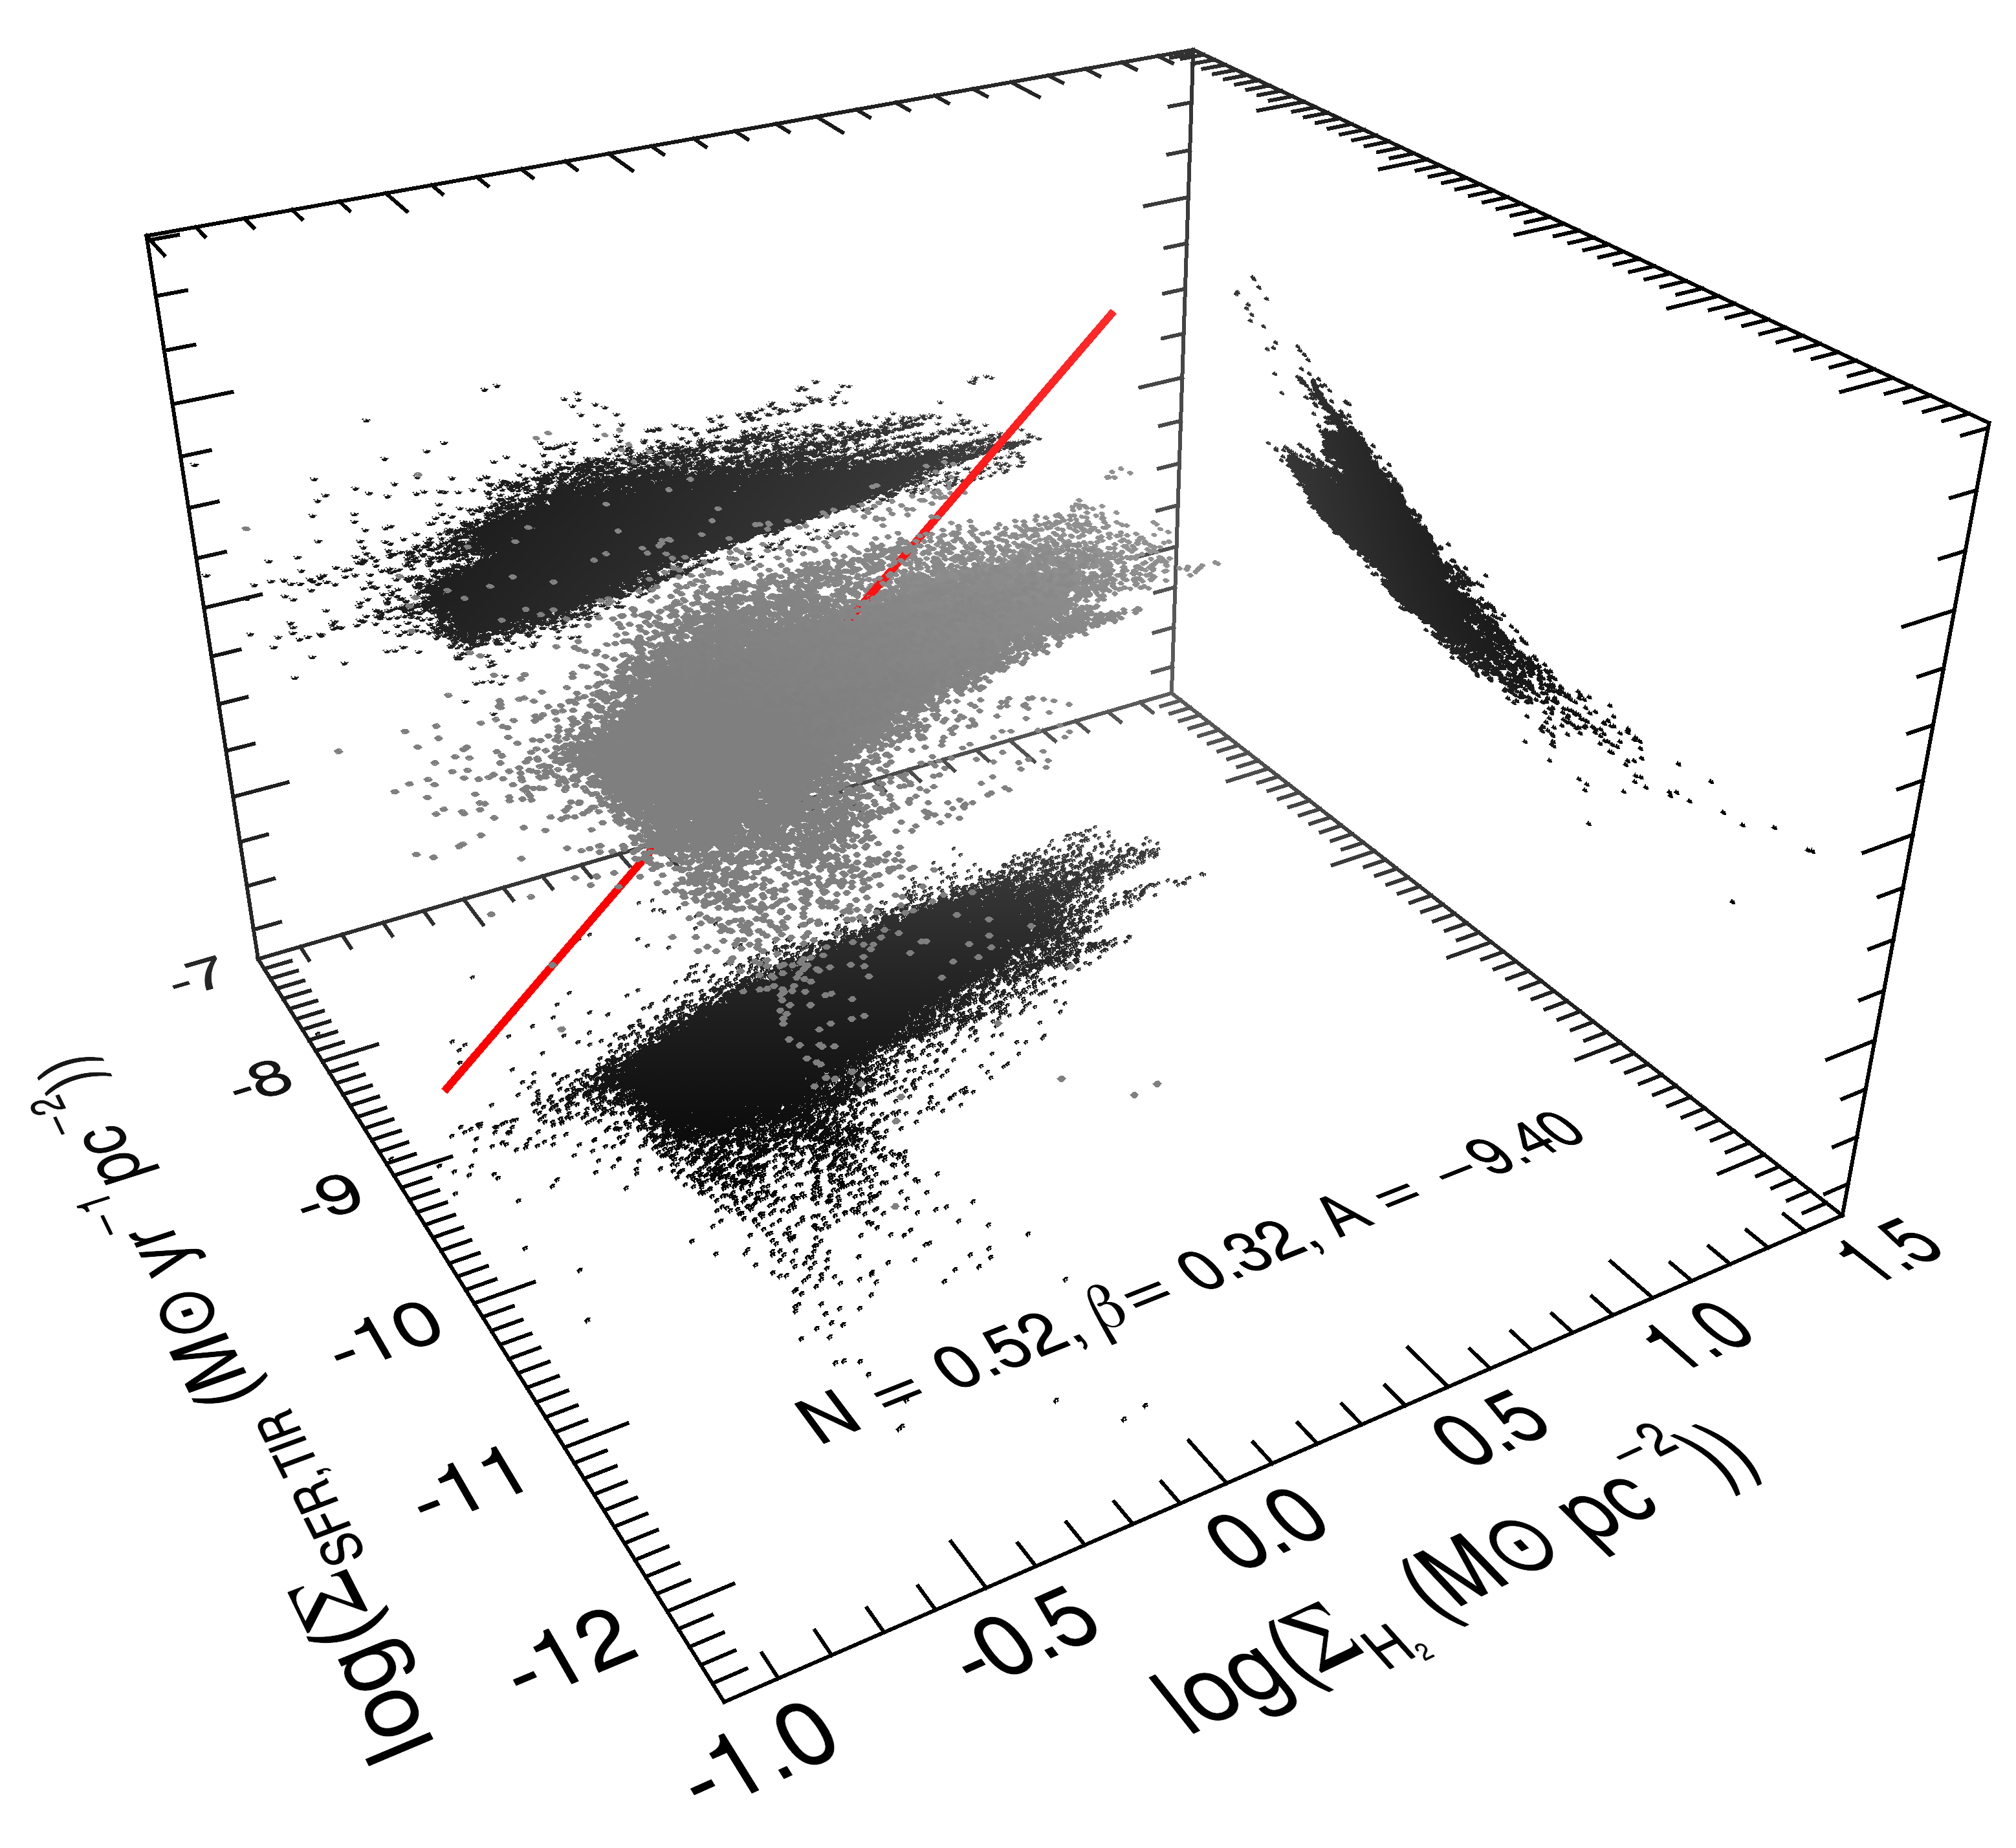
\includegraphics[width=\textwidth]{../image_paper1/es_tot_fir_vs_h2.png}
        \caption{Surface density of SFR(TIR) vs surface density of H$_2$ and surface density of stellar mass ($z$-axis) }
        \label{fig:es,all,fir,h2}
    \end{subfigure}
    \hfill
    \begin{subfigure}[b]{0.5\textwidth}
        \centering
        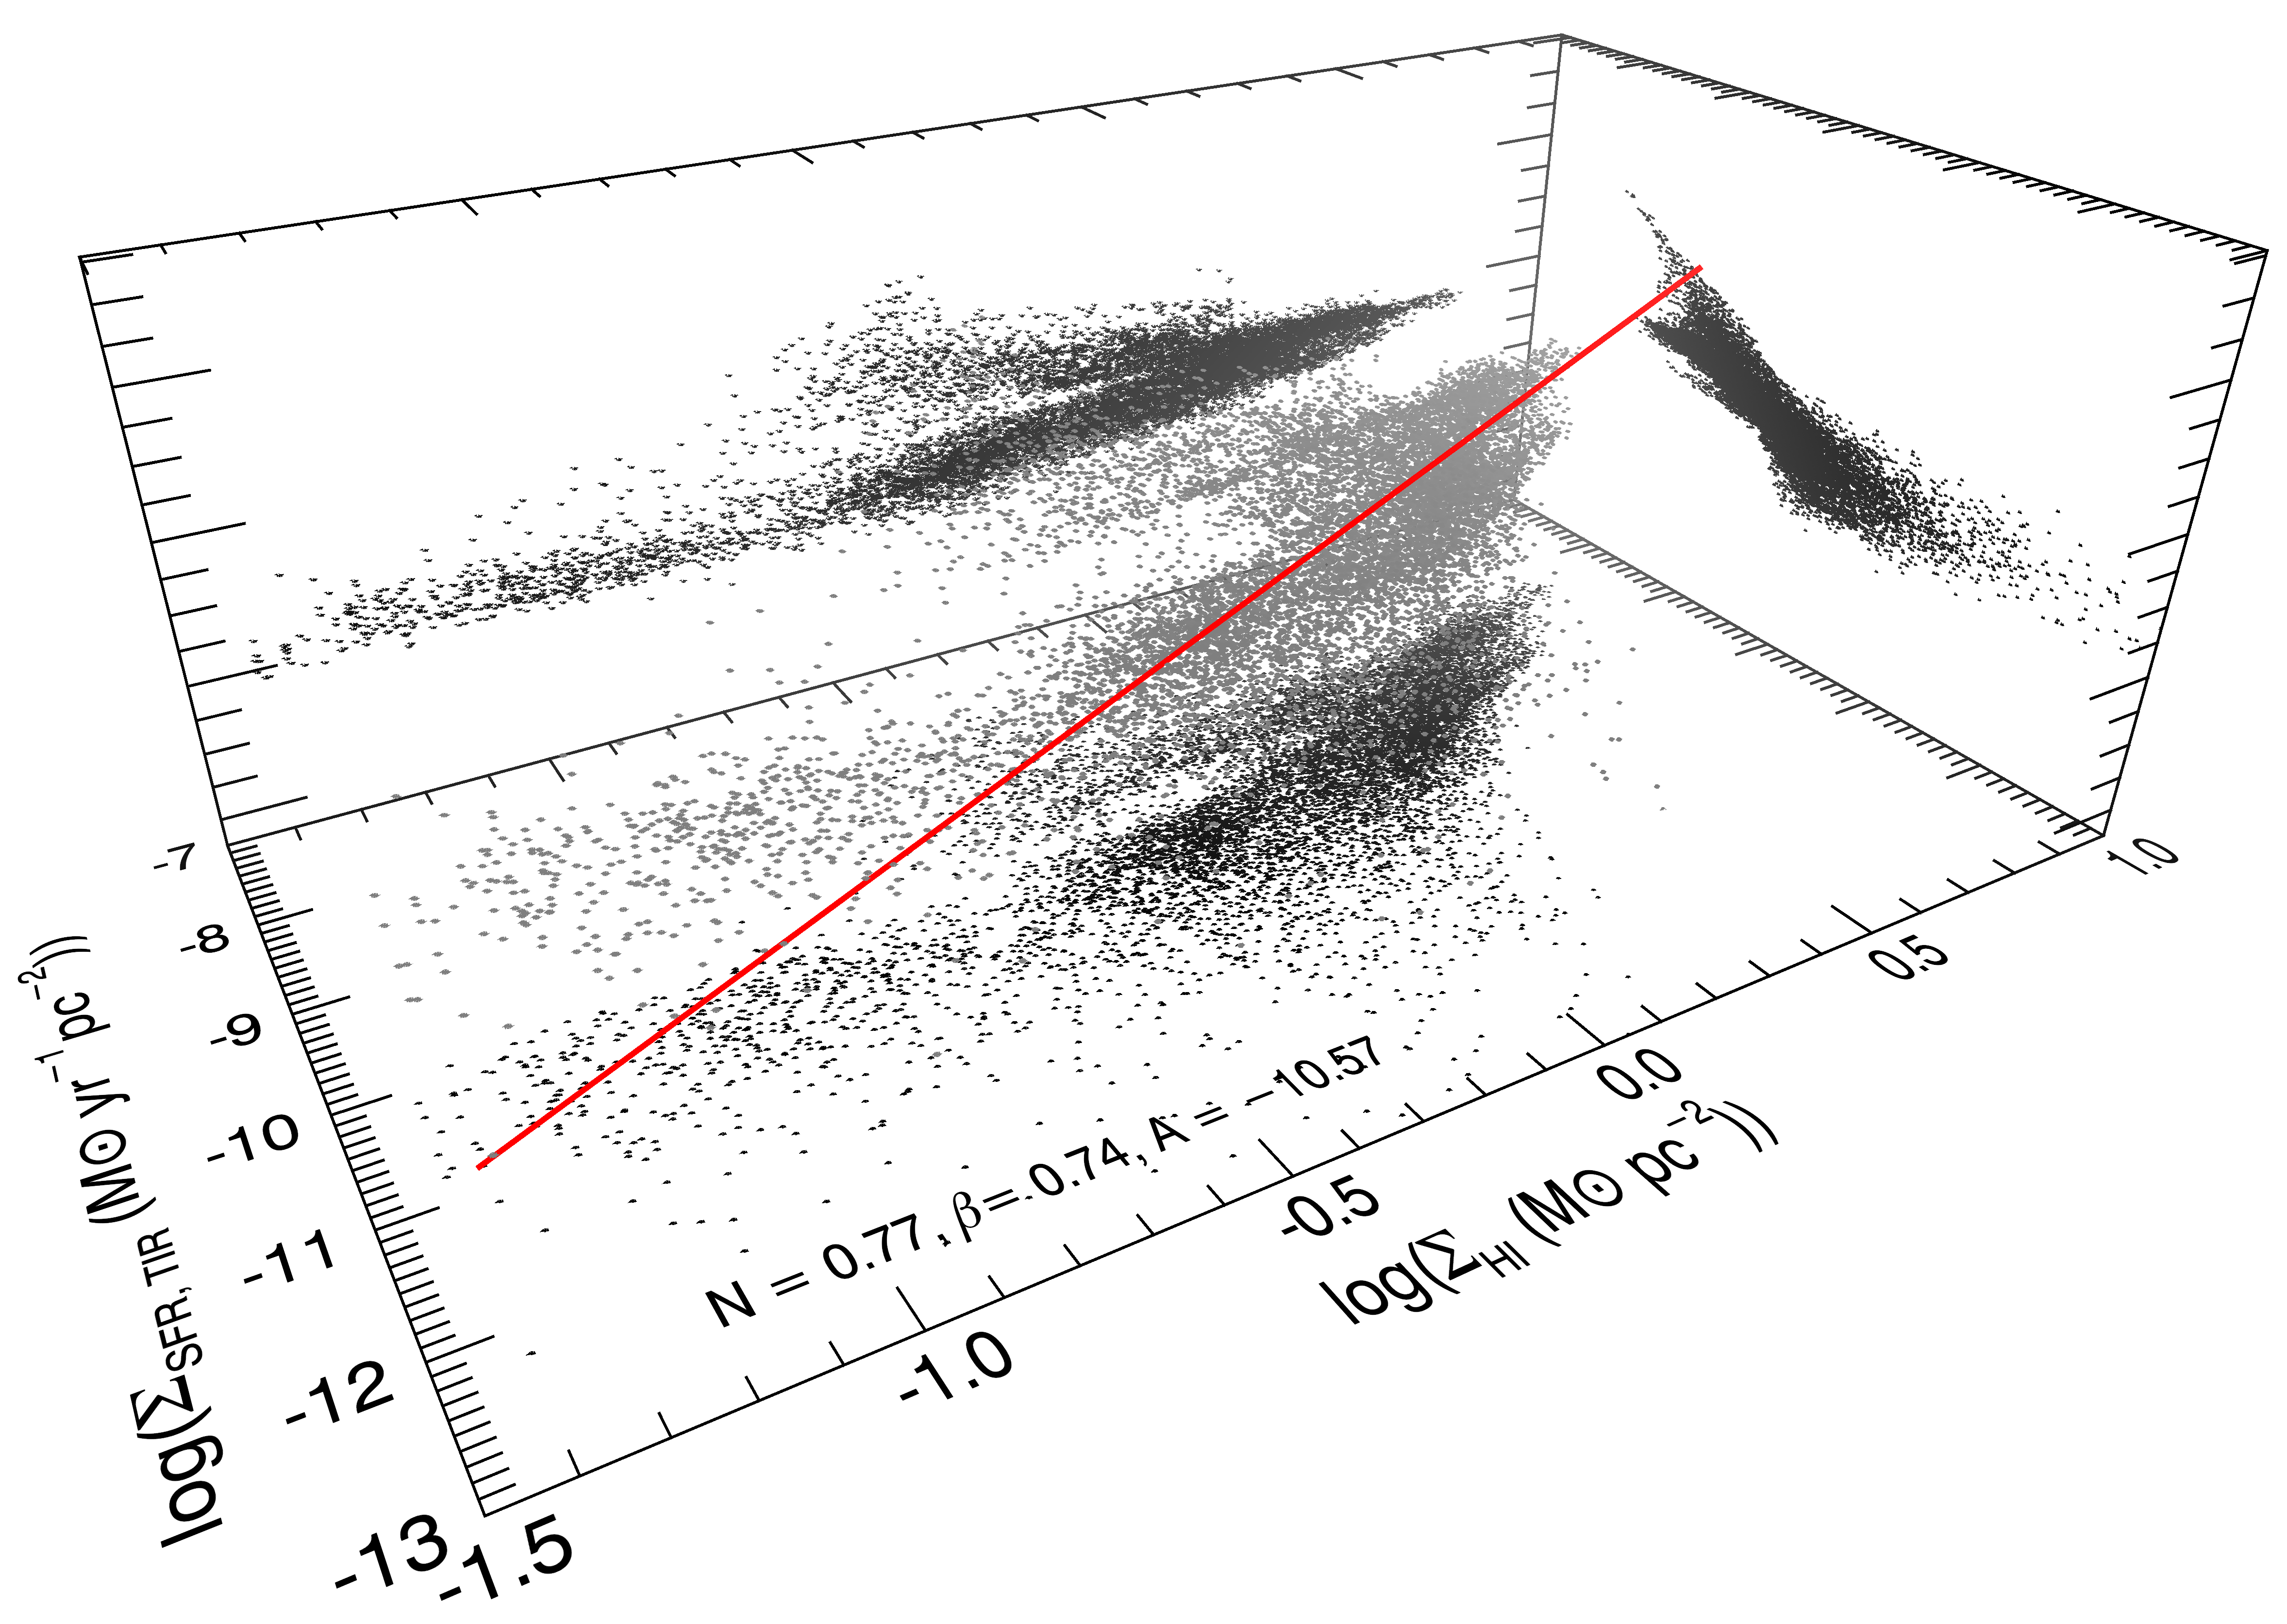
\includegraphics[width=\textwidth]{../image_paper1/es_tot_fir_vs_hi2.png}
        \caption{Surface density of SFR(TIR) vs surface density of H\,{\sc I} and surface density of stellar mass ($z$-axis) }
        \label{fig:es,all,fir,hi}
    \end{subfigure}
    \hfill
   \begin{subfigure}[b]{0.5\textwidth}
        \centering
        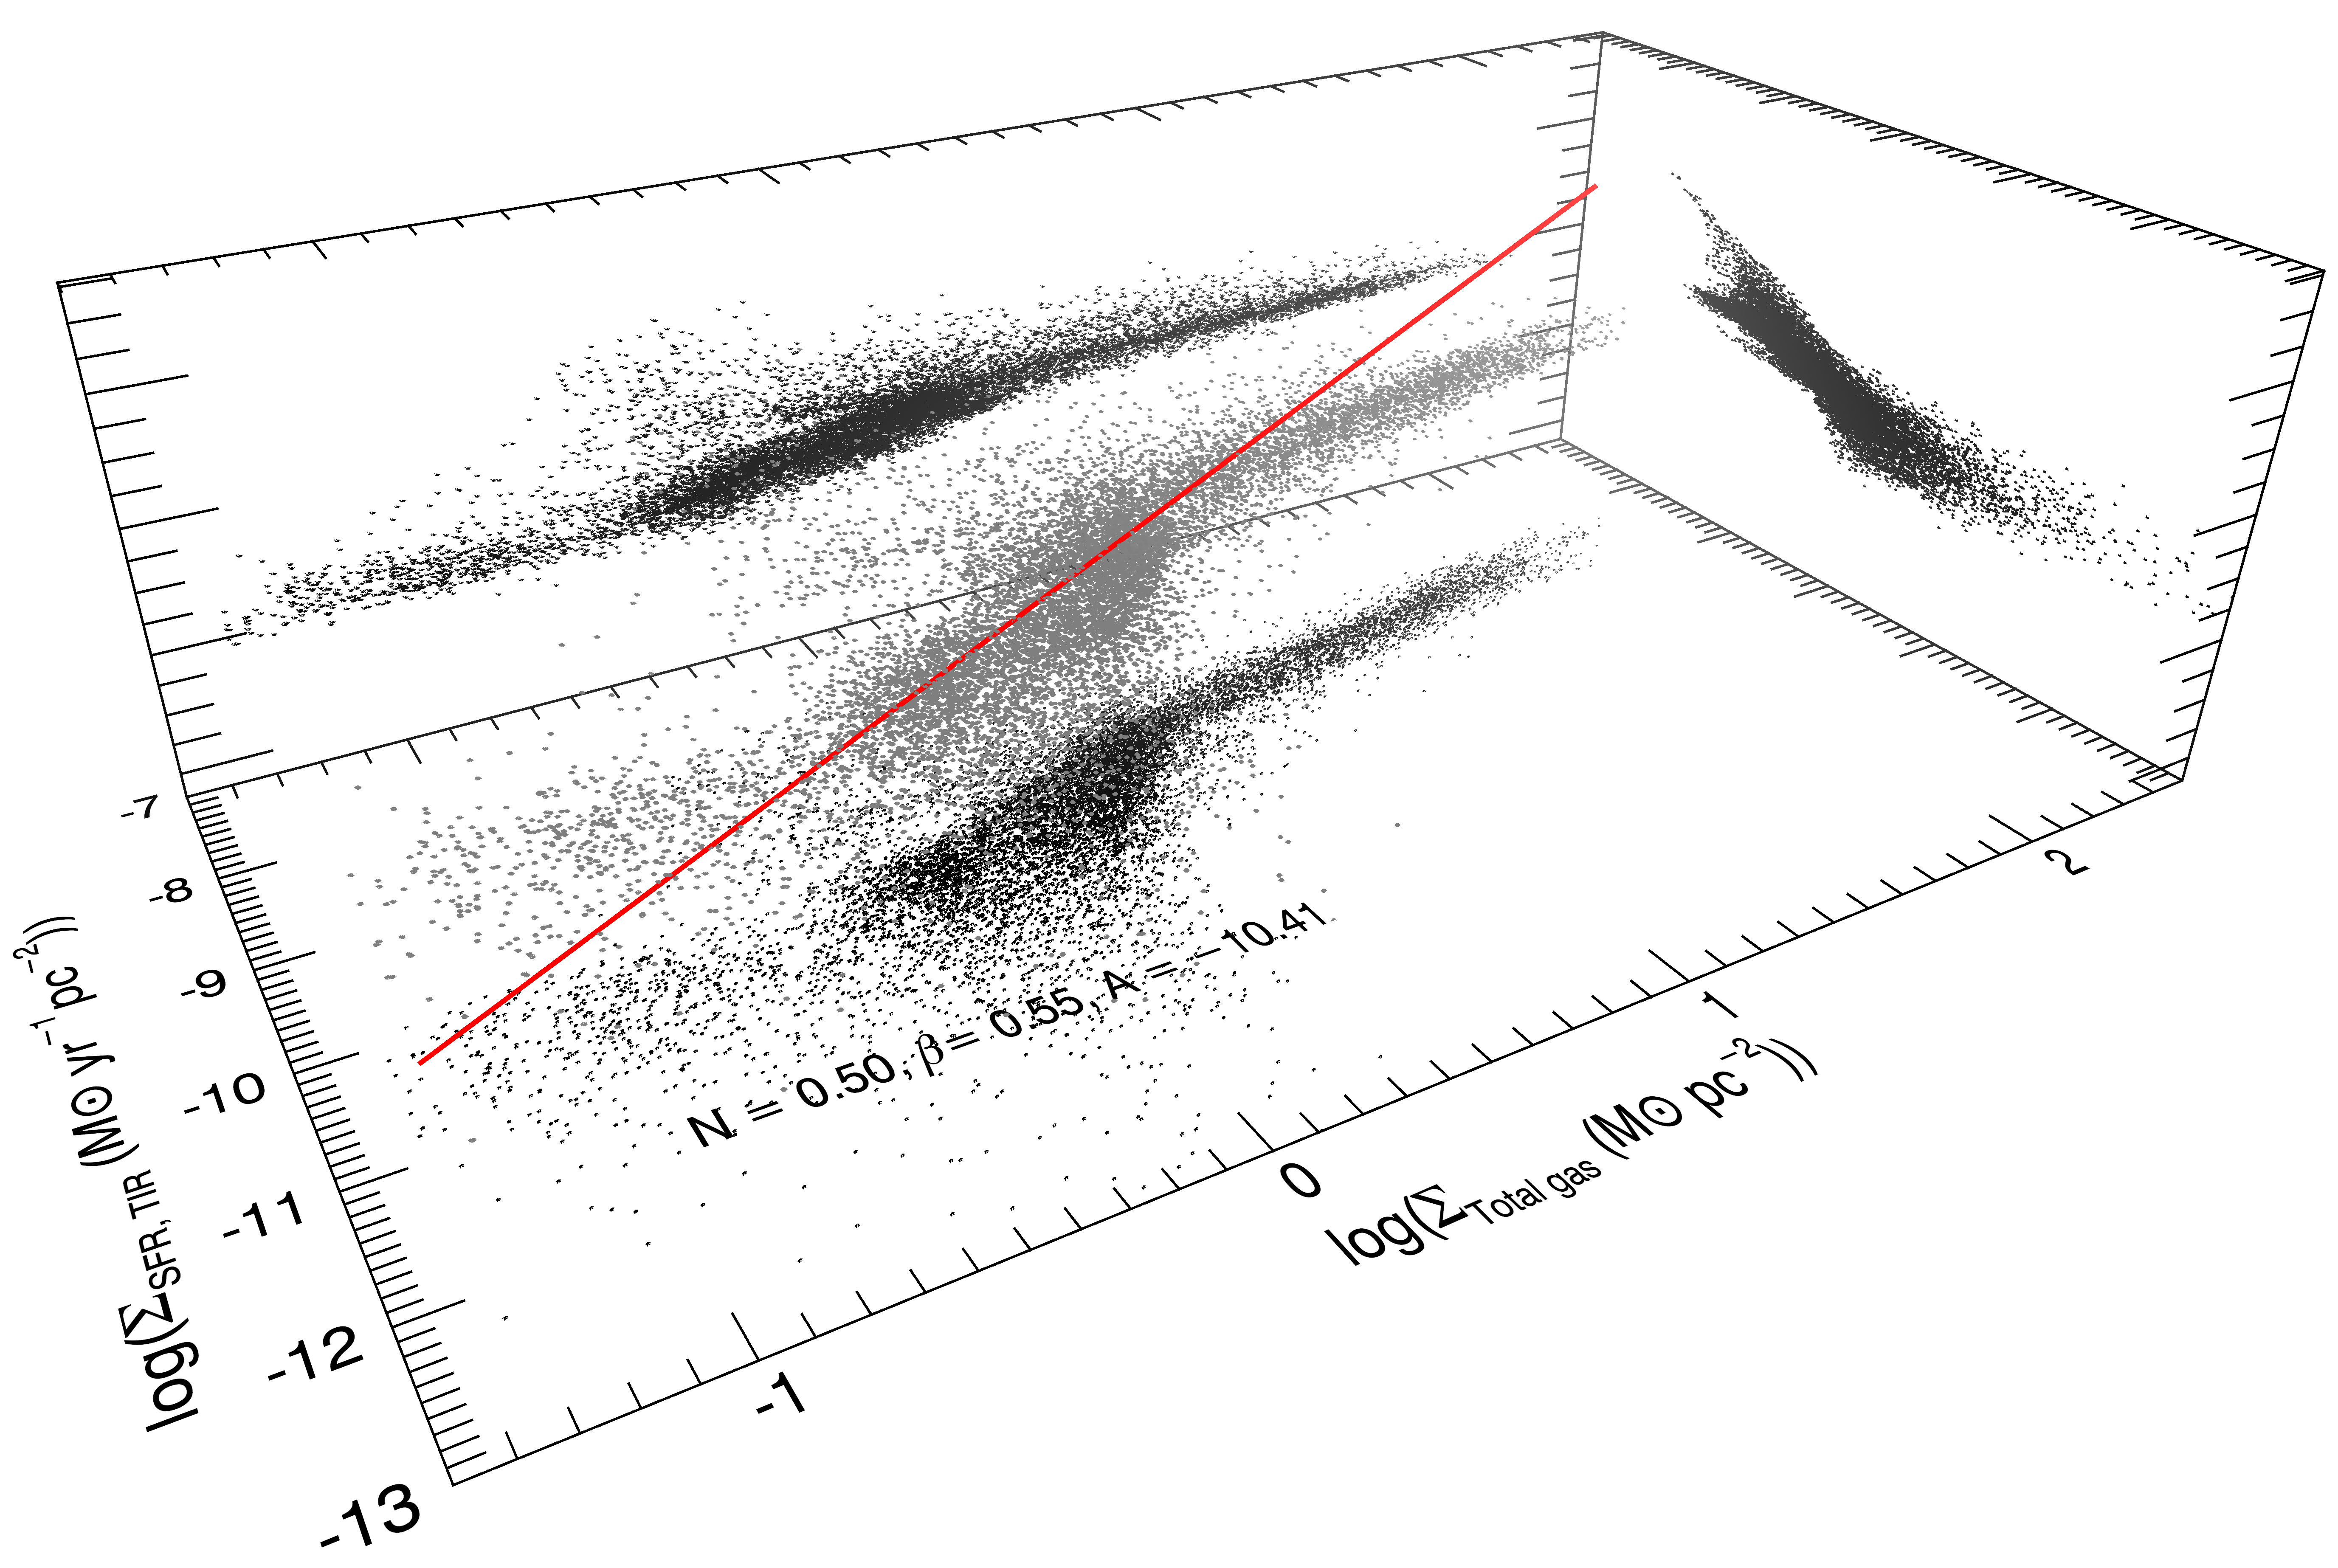
\includegraphics[width=\textwidth]{../image_paper1/es_tot_fir_vs_tot2_f.png}
        \caption{Surface density of SFR(TIR) vs surface density of total gas and surface density of stellar mass ($z$-axis)}
        \label{fig:es,all,fir,tot}
    \end{subfigure}
       \caption{Same as Figure~\ref{fig:es,all,fuv,tot}. Here, from top to bottom plots show the surface density of the SFR(TIR) vs. surface density of H$_2$, surface density of H\,{\sc I}, and the surface density of total gas, respectively. As in Figure~\ref{fig:ks_all}, the analyses use different pixel sizes: each point in the plots with the surface density of H$_2$ as a tracer of gas mass represents a region of size $\sim$30~pc and each point in the plots with the surface density of H\,{\sc I} or total gas mass represents a region of size $\sim$155~pc. Solid lines show the best fit, using the mean value of the ranges in Table~\ref{table:res}.}
       \label{fig:es,fir}
\end{figure*}


\begin{figure*}
    \centering
     \begin{subfigure}[b]{0.5\textwidth}
        \centering
        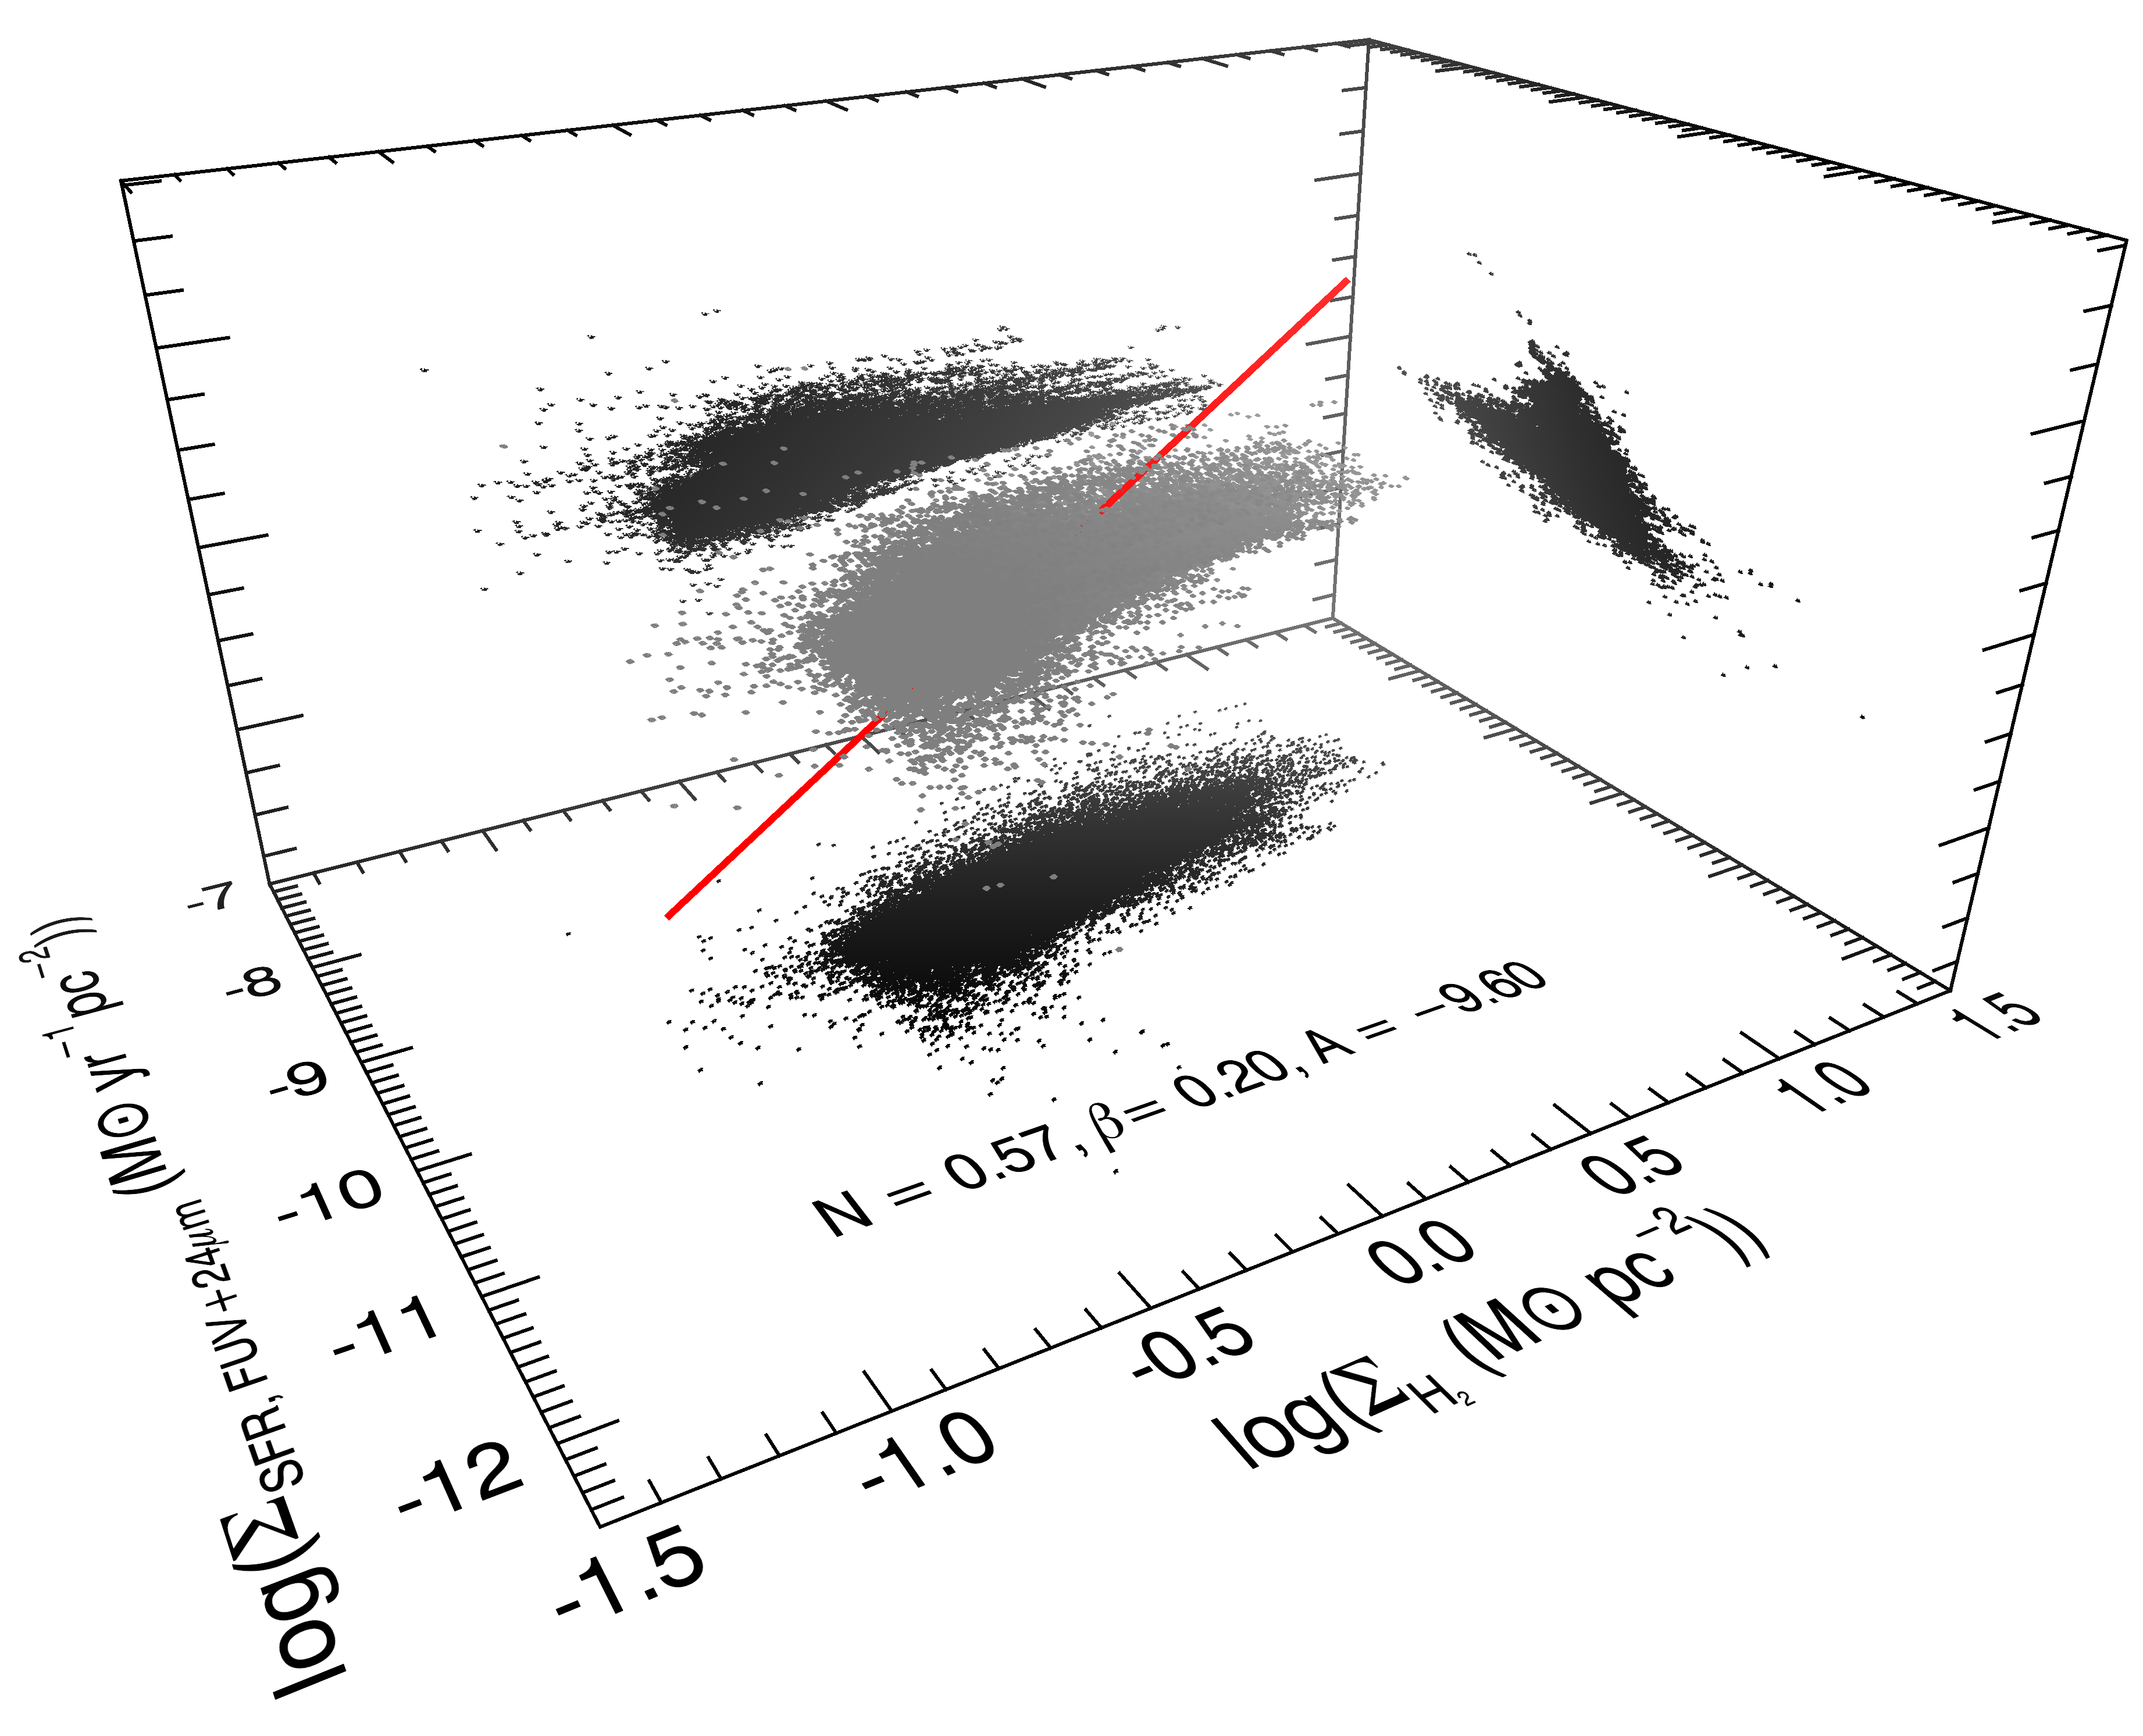
\includegraphics[width=\textwidth]{../image_paper1/es_tot_fuv_vs_h22_f.png}
        \caption{Surface density of SFR(FUV+24~$\mu$m) vs surface density of H$_2$ and surface density of stellar mass ($z$-axis)}
        \label{fig:es,all,fuv,h2}
    \end{subfigure}
     \hfill
   \begin{subfigure}[b]{0.5\textwidth}
        \centering
        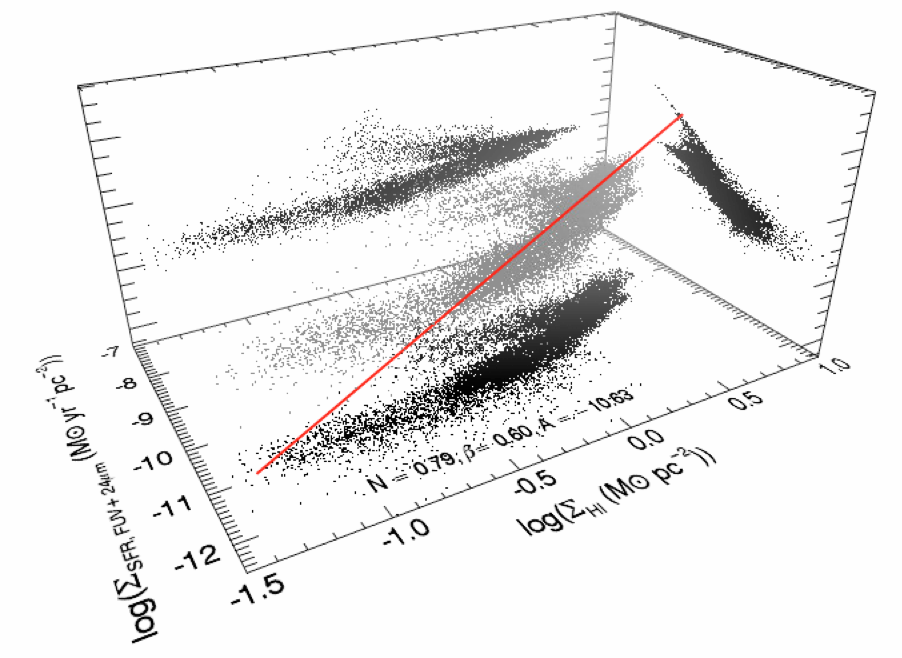
\includegraphics[width=\textwidth]{../image_paper1/es_tot_fuv_vs_hi2.png}
        \caption{Surface density of SFR(FUV+24~$\mu$m) vs surface density of H\,{\sc I} and surface density of stellar mass ($z$-axis)}
        \label{fig:es,all,fuv,hi}
    \end{subfigure}
   \caption{Same as Figure~\ref{fig:es,fir}, but in this figure we used FUV + 24~$\mu$m as a tracer of the SFR. The plot of the surface density of the SFR(FUV+24~$\mu$m) vs the surface density of the total gas is shown in Figure~\ref{fig:es,all,fuv,tot} in the main text.}
\end{figure*}

         
\begin{figure*}
  \centering
   \begin{subfigure}[b]{0.5\textwidth}
        \centering
        \includegraphics[width=\textwidth]{../image_paper1/es_tot_halpha_vs_h22_f.png}
        \caption{Surface density of SFR(H$\alpha$+24~$\mu$m) vs surface density of H$_2$ and surface density of stellar mass ($z$-axis)}
        \label{fig:es,all,halpha,h2}
    \end{subfigure}
     \hfill
      \begin{subfigure}[b]{0.5\textwidth}
        \centering
        \includegraphics[width=\textwidth]{../image_paper1/es_tot_halpha_vs_hi2.png}
        \caption{Surface density of SFR(H$\alpha$+24~$\mu$m) vs surface density of H\,{\sc I} and surface density of stellar mass ($z$-axis)}
        \label{fig:es,all,halpha,hi}
    \end{subfigure}
    \hfill
    \begin{subfigure}[b]{0.5\textwidth}
        \centering
        \includegraphics[width=\textwidth]{../image_paper1/es_tot_halpha_vs_tot2_f.png}
        \caption{Surface density of SFR(H$\alpha$+24~$\mu$m) vs. surface density of total gas and surface density of stellar mass ($z$-axis)}
        \label{fig:es,all,halpha,tot}
    \end{subfigure}
    \caption{Same as Figure~\ref{fig:es,fir}, but in this figure we used H$\alpha$ + 24~$\mu$m as a tracer of the SFR.}
\end{figure*}


\section{Results of training for one-dimensional self-organizing maps}
\label{app: high_Z_1d_soms}
As mentioned in Sec.~\ref{sec: 1D}, we changed the size of the SOM from $1\times2$ to $1\times22$. In that section we show some example of the results, here we show the rest of the maps to monitor the changes in the map in various sizes.

\label{app: 1d}
    \begin{figure}
        \begin{subfigure}[b]{0.5\textwidth}
            \centering
            \includegraphics[width=\textwidth]{../image_paper2/1d/apps/dist_1_by_4.png}
            %\caption{$1\times4$ weight map}
             %\label{fig: 1by4T}
        \end{subfigure}
        \hfill
        \begin{subfigure}[b]{0.5\textwidth}
             \includegraphics[width=\textwidth]{../image_paper2/1d/apps/hit_t_1_by_4.png}
             %\caption{$1\times4$ hits map}
             %\label{fig: 1by4Thits}
        \end{subfigure}
                \caption{Results of training network in $1\times4$~grid.}
         \label{fig: 1by4T}
    \end{figure}
    
    \begin{figure}
        \begin{subfigure}[b]{0.5\textwidth}
            \centering
            \includegraphics[width=\textwidth]{../image_paper2/1d/apps/dist_1_by_5.png}
            %\caption{$1\times5$ weight map}
             %\label{fig: 1by5T}
        \end{subfigure}
        \hfill
        \begin{subfigure}[b]{0.5\textwidth}
             \includegraphics[width=\textwidth]{../image_paper2/1d/apps/hit_t_1_by_5.png}
             %\caption{$1\times5$ hits map}
             %\label{fig: 1by5Thits}
        \end{subfigure}
                \caption{Results of training network in $1\times5$~grid.}
         \label{fig: 1by5T}
    \end{figure}
    
    \begin{figure}
        \begin{subfigure}[b]{0.5\textwidth}
            \centering
            \includegraphics[width=\textwidth]{../image_paper2/1d/apps/dist_1_by_6.png}
            %\caption{$1\times6$ weight map}
             %\label{fig: 1by6T}
        \end{subfigure}
        \hfill
        \begin{subfigure}[b]{0.5\textwidth}
             \includegraphics[width=\textwidth]{../image_paper2/1d/apps/hit_t_1_by_6.png}
             %\caption{$1\times6$ hits map}
             %\label{fig: 1by6Thits}
        \end{subfigure}
                \caption{Results of training network in $1\times6$~grid.}
         \label{fig: 1by6T}
    \end{figure}
    
    \begin{figure}
        \begin{subfigure}[b]{0.5\textwidth}
            \centering
            \includegraphics[width=\textwidth]{../image_paper2/1d/apps/dist_1_by_7.png}
            %\caption{$1\times7$ weight map}
             %\label{fig: 1by7T}
        \end{subfigure}
        \hfill
        \begin{subfigure}[b]{0.5\textwidth}
             \includegraphics[width=\textwidth]{../image_paper2/1d/apps/hit_t_1_by_7.png}
             %\caption{$1\times7$ hits map}
             %\label{fig: 1by7Thits}
        \end{subfigure}
                \caption{Results of training network in $1\times7$~grid.}
         \label{fig: 1by7T}
    \end{figure}
    
    \begin{figure}
        \begin{subfigure}[b]{0.5\textwidth}
            \centering
            \includegraphics[width=\textwidth]{../image_paper2/1d/apps/dist_1_by_8.png}
            %\caption{$1\times8$ weight map}
             %\label{fig: 1by8T}
        \end{subfigure}
        \hfill
        \begin{subfigure}[b]{0.5\textwidth}
             \includegraphics[width=\textwidth]{../image_paper2/1d/apps/hit_t_1_by_8.png}
             %\caption{$1\times8$ hits map}
             %\label{fig: 1by8Thits}
        \end{subfigure}
                \caption{Results of training network in $1\times8$~grid.}
         \label{fig: 1by8T}
    \end{figure}
    
    \begin{figure}
        \begin{subfigure}[b]{0.5\textwidth}
            \centering
            \includegraphics[width=\textwidth]{../image_paper2/1d/apps/dist_1_by_9.png}
            %\caption{$1\times9$ weight map}
             %\label{fig: 1by9T}
        \end{subfigure}
        \hfill
        \begin{subfigure}[b]{0.5\textwidth}
             \includegraphics[width=\textwidth]{../image_paper2/1d/apps/hit_t_1_by_9.png}
             %\caption{$1\times9$ hits map}
             %\label{fig: 1by9Thits}
        \end{subfigure}
                \caption{Results of training network in $1\times9$~grid.}
         \label{fig: 1by9T}
    \end{figure}

    \begin{figure}
        \begin{subfigure}[b]{0.5\textwidth}
            \centering
            \includegraphics[width=\textwidth,height=2.5cm]{../image_paper2/1d/apps/dist_1_by_10.png}
            %\caption{$1\times10$ weight map}
             %\label{fig: 1by10T}
        \end{subfigure}
        \hfill
        \begin{subfigure}[b]{0.5\textwidth}
             \includegraphics[width=\textwidth,height=2.5cm]{../image_paper2/1d/apps/hit_t_1_by_10.png}
             %\caption{$1\times10$ hits map}
             %\label{fig: 1by10Thits}
        \end{subfigure}
                \caption{Results of training network in $1\times10$~grid.}
         \label{fig: 1by10T}
    \end{figure}

    \begin{figure}
        \begin{subfigure}[b]{0.5\textwidth}
            \centering
            \includegraphics[width=\textwidth,height=2.5cm]{../image_paper2/1d/apps/dist_1_by_11.png}
            %\caption{$1\times11$ weight map}
             %\label{fig: 1by11T}
        \end{subfigure}
        \hfill
        \begin{subfigure}[b]{0.5\textwidth}
             \includegraphics[width=\textwidth,height=2.5cm]{../image_paper2/1d/apps/hit_t_1_by_11.png}
             %\caption{$1\times11$ hits map}
             %\label{fig: 1by11Thits}
        \end{subfigure}
                \caption{Results of training network in $1\times11$~grid.}
         \label{fig: 1by11T}
    \end{figure}
    

    \begin{figure}
        \begin{subfigure}[b]{0.5\textwidth}
            \centering
            \includegraphics[width=\textwidth,height=2.5cm]{../image_paper2/1d/apps/dist_1_by_12.png}
            %\caption{$1\times12$ weight map}
             %\label{fig: 1by12T}
        \end{subfigure}
        \hfill
        \begin{subfigure}[b]{0.5\textwidth}
             \includegraphics[width=\textwidth,height=2.5cm]{../image_paper2/1d/apps/hit_t_1_by_12.png}
             %\caption{$1\times12$ hits map}
             %\label{fig: 1by12Thits}
        \end{subfigure}
                \caption{Results of training network in $1\times12$~grid.}
         \label{fig: 1by12T}
    \end{figure}

    \begin{figure}
        \begin{subfigure}[b]{0.5\textwidth}
            \centering
            \includegraphics[width=\textwidth,height=2.5cm]{../image_paper2/1d/apps/dist_1_by_15.png}
            %\caption{$1\times15$ weight map}
             %\label{fig: 1by15T}
        \end{subfigure}
        \hfill
        \begin{subfigure}[b]{0.5\textwidth}
             \includegraphics[width=\textwidth,height=2.5cm]{../image_paper2/1d/apps/hit_t_1_by_15.png}
             %\caption{$1\times15$ hits map}
             %\label{fig: 1by15Thits}
        \end{subfigure}
                \caption{Results of training network in $1\times15$~grid.}
         \label{fig: 1by15T}
    \end{figure}

    \begin{figure}
        \begin{subfigure}[b]{0.5\textwidth}
            \centering
            \includegraphics[width=\textwidth,height=2.5cm]{../image_paper2/1d/apps/dist_1_by_20.png}
            %\caption{$1\times20$ weight map}
             %\label{fig: 1by20T}
        \end{subfigure}
        \hfill
        \begin{subfigure}[b]{0.5\textwidth}
             \includegraphics[width=\textwidth,height=2.5cm]{../image_paper2/1d/apps/hit_t_1_by_20.png}
             %\caption{$1\times20$ hits map}
             %\label{fig: 1by20Thits}
        \end{subfigure}
                \caption{Results of training network in $1\times20$~grid.}
         \label{fig: 1by20T}
    \end{figure}
    

 \chapter{More results from the fitting of the extended Schmidt law}
\pagestyle{plain}
\label{app:es,figs}
\myappendices{
Section~\ref{sec: sfl} discusses testing the extended Schmidt law and shows results for one SFR/gas tracer combination. Here we present the plots for the remaining SFR/gas tracer combinations.


\begin{figure*}
    \centering
    \begin{subfigure}[b]{0.5\textwidth}
        \centering
        \includegraphics[width=\textwidth]{../image_paper1/es_tot_fir_vs_h2.png}
        \caption{Surface density of SFR(TIR) vs surface density of H$_2$ and surface density of stellar mass ($z$-axis) }
        \label{fig:es,all,fir,h2}
    \end{subfigure}
    \hfill
    \begin{subfigure}[b]{0.5\textwidth}
        \centering
        \includegraphics[width=\textwidth]{../image_paper1/es_tot_fir_vs_hi2.png}
        \caption{Surface density of SFR(TIR) vs surface density of H\,{\sc I} and surface density of stellar mass ($z$-axis) }
        \label{fig:es,all,fir,hi}
    \end{subfigure}
    \hfill
   \begin{subfigure}[b]{0.5\textwidth}
        \centering
        \includegraphics[width=\textwidth]{../image_paper1/es_tot_fir_vs_tot2_f.png}
        \caption{Surface density of SFR(TIR) vs surface density of total gas and surface density of stellar mass ($z$-axis)}
        \label{fig:es,all,fir,tot}
    \end{subfigure}
       \caption{Same as Figure~\ref{fig:es,all,fuv,tot}. Here, from top to bottom plots show the surface density of the SFR(TIR) vs. surface density of H$_2$, surface density of H\,{\sc I}, and the surface density of total gas, respectively. As in Figure~\ref{fig:ks_all}, the analyses use different pixel sizes: each point in the plots with the surface density of H$_2$ as a tracer of gas mass represents a region of size $\sim$30~pc and each point in the plots with the surface density of H\,{\sc I} or total gas mass represents a region of size $\sim$155~pc. Solid lines show the best fit, using the mean value of the ranges in Table~\ref{table:res}.}
       \label{fig:es,fir}
\end{figure*}


\begin{figure*}
    \centering
     \begin{subfigure}[b]{0.5\textwidth}
        \centering
        \includegraphics[width=\textwidth]{../image_paper1/es_tot_fuv_vs_h22_f.png}
        \caption{Surface density of SFR(FUV+24~$\mu$m) vs surface density of H$_2$ and surface density of stellar mass ($z$-axis)}
        \label{fig:es,all,fuv,h2}
    \end{subfigure}
     \hfill
   \begin{subfigure}[b]{0.5\textwidth}
        \centering
        \includegraphics[width=\textwidth]{../image_paper1/es_tot_fuv_vs_hi2.png}
        \caption{Surface density of SFR(FUV+24~$\mu$m) vs surface density of H\,{\sc I} and surface density of stellar mass ($z$-axis)}
        \label{fig:es,all,fuv,hi}
    \end{subfigure}
   \caption{Same as Figure~\ref{fig:es,fir}, but in this figure we used FUV + 24~$\mu$m as a tracer of the SFR. The plot of the surface density of the SFR(FUV+24~$\mu$m) vs the surface density of the total gas is shown in Figure~\ref{fig:es,all,fuv,tot} in the main text.}
\end{figure*}

         
\begin{figure*}
  \centering
   \begin{subfigure}[b]{0.5\textwidth}
        \centering
        \includegraphics[width=\textwidth]{../image_paper1/es_tot_halpha_vs_h22_f.png}
        \caption{Surface density of SFR(H$\alpha$+24~$\mu$m) vs surface density of H$_2$ and surface density of stellar mass ($z$-axis)}
        \label{fig:es,all,halpha,h2}
    \end{subfigure}
     \hfill
      \begin{subfigure}[b]{0.5\textwidth}
        \centering
        \includegraphics[width=\textwidth]{../image_paper1/es_tot_halpha_vs_hi2.png}
        \caption{Surface density of SFR(H$\alpha$+24~$\mu$m) vs surface density of H\,{\sc I} and surface density of stellar mass ($z$-axis)}
        \label{fig:es,all,halpha,hi}
    \end{subfigure}
    \hfill
    \begin{subfigure}[b]{0.5\textwidth}
        \centering
        \includegraphics[width=\textwidth]{../image_paper1/es_tot_halpha_vs_tot2_f.png}
        \caption{Surface density of SFR(H$\alpha$+24~$\mu$m) vs. surface density of total gas and surface density of stellar mass ($z$-axis)}
        \label{fig:es,all,halpha,tot}
    \end{subfigure}
    \caption{Same as Figure~\ref{fig:es,fir}, but in this figure we used H$\alpha$ + 24~$\mu$m as a tracer of the SFR.}
\end{figure*}


}
 \chapter{2-Dimensional networks from subsets of M31}
\pagestyle{plain}
\label{sec: app_2d_soms_SOMN}
\newpage
\myappendices{

        We removed IRAC 5.7 $\mu$m; \sii~continuum and \oiii~continuum; PAH8.3 $\mu$m, PAH12.0 $\mu$m, PAH17.0 $\mu$m, \oiii~continuum, stellar mass and metallicity from subset 0, and generated subset samples 2 to 4, respectively (Tables~\ref{tab: subset2} to~\ref{tab: subset4}).
        In Fig.~\ref{fig: subset2}, which is the SOM results from data listed in Table~\ref{tab: subset2}, distance between positions of the region 7, and region 3 is much larger compare to the one in Fig.~\ref{fig: all_derived_ones}. 
        IRAC 5.7~$\mu$m flux in the region 7 and the region 3 is similar to each other. 
        Therefore, removing flux from IRAC 5.7 $\mu$m removed the one source of similarity in these two regions and they moved further from each other in the SOM.
        For subset sample 7 (Table~\ref{tab: subset7}) we removed \sii~flux, SPIRE 250 and 500~$\mu$m and TIR emission from subset 2 (~\ref{tab: subset5}).
        The positions of the regions 2 and 9 are closer to each other, but the weight distance between them is much higher (the colours between them are became almost black). 
        In general by removing IRAC 5.7 $\mu$m  flux data from the input data, the colours between regions become much more darker.
      
        In Fig.~\ref{fig: subset3}, the positions from the region 9 is much closer to the positions of the regions 4 and 7. 
        Since region 4 and 5 have a similar \oiii~and \sii~continuum fluxes, by removing these two values from the input data distance between regions 4 and 5 became much smaller.
        The positions of the regions 2 and 6 are closer together, but the colours between their neurons are darker.
        The wining neurons for regions 1 and 9 are moved further from each other, but the colours between them are slightly lighter. 
        moreover, similar to regions 4 and 5, \oiii~and \sii~continuum fluxes for regions 1 and 9, and regions 8 and 6 are similar to each other, and removing these two values from input data, reduces the similarity between these regions. Therefore, they moved further from each other. 
         \import{../image_paper3/text_files/tables/}{subset2.tex}
        \import{../image_paper3/text_files/image_texts/}{subset2.tex}
        \import{../image_paper3/text_files/tables/}{subset3.tex}
        \import{../image_paper3/text_files/image_texts/}{subset3.tex}
        
        In the results from the subset 4 in Fig.~\ref{fig: subset4}, regions 8 and 6 moved closer to each other. 
        These two regions have distinct metallicity, removing metallicity from input data caused these two stay in a closer neurons. 
        Since regions 1 and 2 have similar metallicity and total PAHs, and their total stellar mass are comparable, removing these values from input data made the position of the regions 1 and 2 moved further from each other. 
        \import{../image_paper3/text_files/tables/}{subset4.tex}
        \import{../image_paper3/text_files/image_texts/}{subset4.tex}
        
        The positions of the region 8 and 5 are moved closer in Fig.~\ref{fig: subset7}.
        Both of these regions are around the inner ring inside the galaxy.
        Therefore, both of them have similar values in most of the input parameters.
        However, they have very different fluxes in IRAC 5.7 $\mu$m and \sii~continuum, which removing these two fluxes from the input data moved their position on the SOM closer.
        TIR luminosity and IRAC 5.7 $\mu$m flux for regions 3 and 5 are different, and removing them from the input data caused the distance between their position decreases. 
        In Fig.~\ref{fig: subset7} the relations between all the other regions are mostly unchanged.
        \import{../image_paper3/text_files/tables/}{subset7.tex}
        \import{../image_paper3/text_files/image_texts/}{subset7.tex}
        }
\chapter[Self-Organizing Map for High-Redshift Galaxies]{Results of Training High-Redshift Galaxies for One-Dimensional Self-Organizing Maps}
\pagestyle{plain}
\label{app: high_Z_1d_soms}
\newpage
\myappendices

As mentioned in Section~\ref{sec: 1D_somz}, we changed the size of the SOM from $1\times2$ to $1\times22$. In that section we show some example of the results, here we show the rest of the maps to monitor the changes in the map in various sizes.

\label{app: 1d}
    \begin{figure}
        \begin{subfigure}[b]{0.5\textwidth}
            \centering
            \includegraphics[width=\textwidth]{../image_paper2/1d/apps/dist_1_by_4.png}
            %\caption{$1\times4$ weight map}
             %\label{fig: 1by4T}
        \end{subfigure}
        \hfill
        \begin{subfigure}[b]{0.5\textwidth}
             \includegraphics[width=\textwidth]{../image_paper2/1d/apps/hit_t_1_by_4.png}
             %\caption{$1\times4$ hits map}
             %\label{fig: 1by4Thits}
        \end{subfigure}
                \caption{Results of training network in $1\times4$~grid.}
         \label{fig: 1by4T}
    \end{figure}
    
    \begin{figure}
        \begin{subfigure}[b]{0.5\textwidth}
            \centering
            \includegraphics[width=\textwidth]{../image_paper2/1d/apps/dist_1_by_5.png}
            %\caption{$1\times5$ weight map}
             %\label{fig: 1by5T}
        \end{subfigure}
        \hfill
        \begin{subfigure}[b]{0.5\textwidth}
             \includegraphics[width=\textwidth]{../image_paper2/1d/apps/hit_t_1_by_5.png}
             %\caption{$1\times5$ hits map}
             %\label{fig: 1by5Thits}
        \end{subfigure}
                \caption{Results of training network in $1\times5$~grid.}
         \label{fig: 1by5T}
    \end{figure}
    
    \begin{figure}
        \begin{subfigure}[b]{0.5\textwidth}
            \centering
            \includegraphics[width=\textwidth]{../image_paper2/1d/apps/dist_1_by_6.png}
            %\caption{$1\times6$ weight map}
             %\label{fig: 1by6T}
        \end{subfigure}
        \hfill
        \begin{subfigure}[b]{0.5\textwidth}
             \includegraphics[width=\textwidth]{../image_paper2/1d/apps/hit_t_1_by_6.png}
             %\caption{$1\times6$ hits map}
             %\label{fig: 1by6Thits}
        \end{subfigure}
                \caption{Results of training network in $1\times6$~grid.}
         \label{fig: 1by6T}
    \end{figure}
    
    \begin{figure}
        \begin{subfigure}[b]{0.5\textwidth}
            \centering
            \includegraphics[width=\textwidth]{../image_paper2/1d/apps/dist_1_by_7.png}
            %\caption{$1\times7$ weight map}
             %\label{fig: 1by7T}
        \end{subfigure}
        \hfill
        \begin{subfigure}[b]{0.5\textwidth}
             \includegraphics[width=\textwidth]{../image_paper2/1d/apps/hit_t_1_by_7.png}
             %\caption{$1\times7$ hits map}
             %\label{fig: 1by7Thits}
        \end{subfigure}
                \caption{Results of training network in $1\times7$~grid.}
         \label{fig: 1by7T}
    \end{figure}
    
    \begin{figure}
        \begin{subfigure}[b]{0.5\textwidth}
            \centering
            \includegraphics[width=\textwidth]{../image_paper2/1d/apps/dist_1_by_8.png}
            %\caption{$1\times8$ weight map}
             %\label{fig: 1by8T}
        \end{subfigure}
        \hfill
        \begin{subfigure}[b]{0.5\textwidth}
             \includegraphics[width=\textwidth]{../image_paper2/1d/apps/hit_t_1_by_8.png}
             %\caption{$1\times8$ hits map}
             %\label{fig: 1by8Thits}
        \end{subfigure}
                \caption{Results of training network in $1\times8$~grid.}
         \label{fig: 1by8T}
    \end{figure}
    
    \begin{figure}
        \begin{subfigure}[b]{0.5\textwidth}
            \centering
            \includegraphics[width=\textwidth]{../image_paper2/1d/apps/dist_1_by_9.png}
            %\caption{$1\times9$ weight map}
             %\label{fig: 1by9T}
        \end{subfigure}
        \hfill
        \begin{subfigure}[b]{0.5\textwidth}
             \includegraphics[width=\textwidth]{../image_paper2/1d/apps/hit_t_1_by_9.png}
             %\caption{$1\times9$ hits map}
             %\label{fig: 1by9Thits}
        \end{subfigure}
                \caption{Results of training network in $1\times9$~grid.}
         \label{fig: 1by9T}
    \end{figure}

    \begin{figure}
        \begin{subfigure}[b]{0.5\textwidth}
            \centering
            \includegraphics[width=\textwidth,height=2.5cm]{../image_paper2/1d/apps/dist_1_by_10.png}
            %\caption{$1\times10$ weight map}
             %\label{fig: 1by10T}
        \end{subfigure}
        \hfill
        \begin{subfigure}[b]{0.5\textwidth}
             \includegraphics[width=\textwidth,height=2.5cm]{../image_paper2/1d/apps/hit_t_1_by_10.png}
             %\caption{$1\times10$ hits map}
             %\label{fig: 1by10Thits}
        \end{subfigure}
                \caption{Results of training network in $1\times10$~grid.}
         \label{fig: 1by10T}
    \end{figure}

    \begin{figure}
        \begin{subfigure}[b]{0.5\textwidth}
            \centering
            \includegraphics[width=\textwidth,height=2.5cm]{../image_paper2/1d/apps/dist_1_by_11.png}
            %\caption{$1\times11$ weight map}
             %\label{fig: 1by11T}
        \end{subfigure}
        \hfill
        \begin{subfigure}[b]{0.5\textwidth}
             \includegraphics[width=\textwidth,height=2.5cm]{../image_paper2/1d/apps/hit_t_1_by_11.png}
             %\caption{$1\times11$ hits map}
             %\label{fig: 1by11Thits}
        \end{subfigure}
                \caption{Results of training network in $1\times11$~grid.}
         \label{fig: 1by11T}
    \end{figure}
    

    \begin{figure}
        \begin{subfigure}[b]{0.5\textwidth}
            \centering
            \includegraphics[width=\textwidth,height=2.5cm]{../image_paper2/1d/apps/dist_1_by_12.png}
            %\caption{$1\times12$ weight map}
             %\label{fig: 1by12T}
        \end{subfigure}
        \hfill
        \begin{subfigure}[b]{0.5\textwidth}
             \includegraphics[width=\textwidth,height=2.5cm]{../image_paper2/1d/apps/hit_t_1_by_12.png}
             %\caption{$1\times12$ hits map}
             %\label{fig: 1by12Thits}
        \end{subfigure}
                \caption{Results of training network in $1\times12$~grid.}
         \label{fig: 1by12T}
    \end{figure}

    \begin{figure}
        \begin{subfigure}[b]{0.5\textwidth}
            \centering
            \includegraphics[width=\textwidth,height=2.5cm]{../image_paper2/1d/apps/dist_1_by_15.png}
            %\caption{$1\times15$ weight map}
             %\label{fig: 1by15T}
        \end{subfigure}
        \hfill
        \begin{subfigure}[b]{0.5\textwidth}
             \includegraphics[width=\textwidth,height=2.5cm]{../image_paper2/1d/apps/hit_t_1_by_15.png}
             %\caption{$1\times15$ hits map}
             %\label{fig: 1by15Thits}
        \end{subfigure}
                \caption{Results of training network in $1\times15$~grid.}
         \label{fig: 1by15T}
    \end{figure}

    \begin{figure}
        \begin{subfigure}[b]{0.5\textwidth}
            \centering
            \includegraphics[width=\textwidth,height=2.5cm]{../image_paper2/1d/apps/dist_1_by_20.png}
            %\caption{$1\times20$ weight map}
             %\label{fig: 1by20T}
        \end{subfigure}
        \hfill
        \begin{subfigure}[b]{0.5\textwidth}
             \includegraphics[width=\textwidth,height=2.5cm]{../image_paper2/1d/apps/hit_t_1_by_20.png}
             %\caption{$1\times20$ hits map}
             %\label{fig: 1by20Thits}
        \end{subfigure}
                \caption{Results of training network in $1\times20$~grid.}
         \label{fig: 1by20T}
    \end{figure}
    
 \end{appendices}


%CV only relevant stuff... not full CV.
 \addcontentsline{toc}{chapter}{Curriculum Vitae}
\chapter*{Curriculum Vitae}
\begin{table}[ht]
\begin{tabular}{ll}
\textbf{Name:} & \firstname{} \lastname\\\\
\textbf{Post-Secondary} & {\sl Doctor of Philosophy,} Astronomy \\
\textbf{Education and}& Western University\\
\textbf{Degrees:}& London, ON\\
& 2012 - 2016\\\\
&{\sl Master of Science,} Astronomy \\
& University of Sussex \\
& Brighton, England\\
& 2011 - 2012\\\\
& {\sl Bachelor of Science,} Physics \\
& Sharif University of Technology \\
& Tehran, Iran \\
& 2006 - 2011\\\\
\textbf{Honours and}& {\sl Western University Graduate Research Scholarship}\\
\textbf{Awards:}&(2012-2016)\\\\
& {\sl Travel Grant for Statistical Challenges in Modern Astronomy VI,}\\
&  Pittsburgh, PA (Spring, 2016)\\\\
% &{\sl Travel Grant for Canadian Astronomical Society Conference (CASCA),} \\
% & Winnipeg, MB (Spring, 2016)\\
&{\sl Scholarship for Utrecht Summer School on Star formation,}\\
&Utrecht, Netherlands (Summer, 2009)\\\\
\textbf{Related Work}& Graduate Research \& Teaching Assistant\\
\textbf{Experience:}& Western University\\
& 2012 - 2016\\\\
% & Instructor for Software Carpentry\\
% & 2015 - 2016\\\\
&Graduate Research Assistant\\
& University of Sussex \\
& 2011 - 2012\\\\
\end{tabular}
\end{table}

\subsubsection*{Publications:}
 \textbf{Rahmani. S}, Lianou. S, Barmby. P, ``{\em Star formation laws in the Andromeda galaxy: gas, stars, metals and the surface density of star formation}'', 2016, MNRAS, 456, 4128\\
\textbf{Rahmani. S}, Teimoorinia. H, Barmby. P, `` {\em Classifying galaxy spectra at $0.5<z<1$: an unsupervised approach}", Submitted to MNRAS, JUNE,2016\\

\subsubsection*{Work in Preparation}
 \textbf{Rahmani. S}, Teimoorinia. H, Peeters. E, Barmby. P, `` {\em Data Mining in nearby galaxies}", In prep.\\

\subsubsection*{Conferences Talks}

{\sl Canadian Astronomical Society Conference (CASCA), Winnipeg, MB}\hfill(2016)
\begin{itemize} 
\item Rahmani, S., Teimoorinia, H., Peeters, E.,  Barmby, P. 2013, ``Data mining in nearby galaxies" 
\end{itemize}

{\sl International Tusi Conference on Astrophysics, devoted to the Maragha Observatory's 750th year
anniversary, Maragha, Iran} \hfill(2009)
\begin{itemize} 
\item Rahmani, S., Mashhoon, M., Moghaddam , A., ``Challenges of brightness variations of Planets: From Geocentric to Heliocentric" 
\end{itemize}
\subsubsection*{Conferences Posters}
{\sl Statistical challenges in Modern Astronomy {\textsc VI}, Pittsburgh, PA}\hfill(2016)
\begin{itemize} 
\item Rahmani, S., Teimoorinia, H., Peeters, E.,  Barmby, P. 2013, ``Data mining in nearby galaxies" 
\end{itemize}

{\sl From galactic to extra galactic star formation (GESF), Marsseile, France}\hfill (2014)
\begin{itemize} 
\item Rahmani, S., Barmby, P. 2013, ``Which Star formation laws in M31?" 
\end{itemize}

{\sl Canadian Astronomical Society Conference (CASCA), University of British Colombia, BC}\hfill (2013)
\begin{itemize} 
\item Rahmani, S., Barmby, P. 2013, ``Effects of Gas Clouds and Existing Stars on Current Star Formation in M31: Testing the Extended Schmidt Law" 
\end{itemize}

\end{document}
